\documentclass[book]{magnolia}

\magtex{tex_driver={pdftex},
        tex_packages={float,caption,titling,epigraph,minitoc,slashbox,tabularx,cancel,pgfplots,xypic,nicefrac},
        tex_pstricks={pstricks,pst-plot}}
\magfiche{document_nom={Cours de Sup},
          auteur_nom={François Fayard},
          auteur_mail={fayard.prof@gmail.com}}
\magcours{cours_matiere={maths},
          cours_niveau={mpsi},
          cours_chapitre_numero={11},
          cours_chapitre={Dérivation}}
\magmisenpage{misenpage_presentation={tikzvelvia},
              misenpage_format={a4},
              misenpage_nbcolonnes={1},
              misenpage_preuve={non},
              misenpage_sol={non}}
\maglieudiff{lieu_lycee={Aux Lazaristes},
             lieu_classe={MPSI 1},
             lieu_annee={2020--2021}}
\magprocess

\title{{\Huge\bf Cours d'Informatique Commune}\\\vspace{1cm}
       \textbf{\Huge Maths Sup}\\\vspace{1cm}
       \textsc{F. Fayard}\\\vspace{1cm}
      %  \includegraphics[width=12cm]{../../Commun/Images/magnolia.jpg}
       }

\mtcsettitle{minitoc}{}
\mtcsettitle{secttoc}{Table des matières}
\mtcsettitle{parttoc}{Table des matières}

\usetikzlibrary{positioning}

\input{vc.tex}

\begin{document}

\maketitle

La version de ce document est la \textsc{\GITAbrHash}.

\tableofcontents


\chapter{Valeur, type, variable}
\setcounter{numeroexercicecours}{1}
\documentclass{magnolia}

\magtex{tex_driver={pdftex},
        tex_packages={xypic}}
\magfiche{document_nom={Cours Python sur les valeurs et types},
          auteur_nom={François Fayard},
          auteur_mail={fayard.prof@gmail.com}}
\magcours{cours_matiere={python},
          cours_niveau={mpsi},
          cours_chapitre_numero={1},
          cours_chapitre={Valeur, type et variable}}
\magmisenpage{}
\maglieudiff{}
\magprocess

\begin{document}
%BEGIN_BOOK
\hfill\includegraphics[width=0.7\textwidth]{../../Commun/Images/maths-cours-tech-calvin.png}\\

\magtoc

\section{Valeur, type}

Le langage Python manipule des valeurs de différents \emph{types}.
Nous rencontrerons d'abord les types numériques~: les \emph{entiers} ainsi que les
\emph{nombres flottants} que l'on utilise pour représenter les réels. Nous verrons
ensuite les \emph{chaines de caractères}, les \emph{booléens} et les \emph{tuples}.

\subsection{Nombre entier}

Nous utiliserons Python le plus souvent dans ce qu'on
appelle le shell ou la boucle interactive. Ce mode est aussi appelé
\og {\sc Repl} \fg pour~: Read, Evaluate, Print, Loop. Autrement dit, lorsqu'on entre
une expression, Python la lit, l'évalue, affiche le résultat, et est
prêt pour l'interaction suivante.\\

On écrit les entiers de manière naturelle. D'une manière générale,
on obtient le type d'une valeur grâce à la fonction \verb_type_. 

\begin{pythoncode}
In [1]: 42
Out[1]: 42

In [2]: type(42)
Out[2]: int
\end{pythoncode}

\noindent Le type des entiers est donc \verb_int_. 
Les opérateurs usuels d'addition \og\verb_+_\fg, de soustraction \og\verb_-_\fg, de
multiplication \og\verb+*+\fg et d'exponentiation \og\verb_**_\fg sont disponibles pour
créer des \emph{expressions} qui sont \emph{évaluées} par l'interpréteur. Ces opérateurs
possèdent différents niveaux de priorité. L'exponentiation est prioritaire sur 
la multiplication. L'addition et la soustraction ont la priorité la plus basse.

\begin{pythoncode}
In [3]: 2 + 3 * 5
Out[3]: 17

In [4]: -1 + 2 ** 8
Out[4]: 255
\end{pythoncode}

\noindent
On utilise les parenthèses pour grouper différentes sous-expressions lorsque les calculs
que l'on souhaite effectuer diffèrent de ceux fixés par les règles de priorité.

\begin{pythoncode}
In [5]: (2 + 3) * 5
Out[5]: 25 
\end{pythoncode}

\noindent
Les différentes règles de priorité sont parfois subtiles. Il est donc souhaitable, pour des raisons de lisibilité,
d'ajouter des parenthèses dès lors que l'évaluation de notre expression repose sur leur
connaissance fine. N'oubliez jamais qu'un programme est écrit pour être lu non seulement par
un ordinateur, mais aussi par des humains, qu'ils soient programmeurs ou correcteurs de
concours. Par exemple, on n'écrira pas \verb_2 ** 2 ** 3_ mais plutôt l'une
des deux expressions suivantes~:

\begin{pythoncode}
In [6]: (2 ** 2) ** 3
Out[6]: 64

In [7]: 2 ** (2 ** 3)
Out[7]: 256
\end{pythoncode}

\noindent 
Ces opérateurs sont des opérateurs \emph{binaires}~: ils nécessitent deux arguments.
Le \textsc{Pep8}, qui fixe les règles de bon usage
en Python, recommande de mettre un espace de part et d'autre de tels opérateurs.
Cependant, lorsqu'on construit des expressions mélangeant des opérateurs ayant
différents niveaux de priorité, il est parfois plus lisible d'omettre cet espace autour des
opérateurs ayant la priorité la plus forte. Par exemple, on écrira \verb!2**10 - 1!.\\

Le symbole \og\verb_-_\fg, utilisé comme opérateur
binaire de soustraction, est aussi utilisé pour la négation. Dans ce cas, c'est
un opérateur \emph{unaire} ne nécessitant qu'une opérande.

\begin{pythoncode}
In [8]: -2 * 3
Out[8]: -6
\end{pythoncode}
\noindent
Contrairement à ce qui se passe dans la plupart des autres langages comme le \textsc{C} ou
OCaml, Python peut représenter des nombres aussi grands que l'on souhaite.
Prenons l'exemple du $n$-ième nombre de Mersenne définit par
$M_n\defeq 2^n-1$. Il est courant de chercher des nombres premiers parmi ces entiers. Le
dixième nombre de Mersenne qui est premier est $M_{89}$ et son calcul ne pose aucun
problème à Python.

\begin{pythoncode}
In [9]: 2**89 - 1
Out[9]: 618970019642690137449562111
\end{pythoncode}
\vspace{1ex}

Python offre deux types de division. Commençons par la division entière. Rappelons le théorème de la division euclienne sur $\Z$~:

\begin{proposition}
Soit $a\in\Z$ et $b\in\Ns$. Alors il existe un unique couple $\p{q,r}\in\Z^2$
tel que
\[a=qb+r \et 0\leq r<b.\]
$q$ est appelé \emph{quotient} de la division euclidienne de $a$ par $b$, et $r$ son
\emph{reste}.
\end{proposition}

\noindent
Par exemple $7 = 2\times 3 + 1$, donc 2 est le quotient de la division
euclidienne de 7 par 3 et son reste est $1$. De même $-7 = (-3)\times 3 + 2$, donc $-3$ est
le quotient de la division euclidienne de $-7$ par 3 et son reste est 2. En Python,
on obtient le quotient de la division euclidienne de $a$ par $b$ avec
\verb_a // b_ et son reste avec \verb_a % b_.

\begin{pythoncode}
In [10]: -7 // 3
Out[10]: -3

In [11]: -7 % 3
Out[11]: 2
\end{pythoncode}

\noindent La division par 0 est une erreur et lève ce
qu'on appelle une \emph{exception}. Même s'il est possible de rattraper les exceptions,
nous ne le ferons pas dans ce cours et une division par 0 aura pour effet de produire
l'erreur suivante~:

\begin{francois}
\begin{pythoncode}
In [12]: 1 // 0
(*@\textcolor{violet}{ZeroDivisionError: integer division or modulo by zero}@*)
\end{pythoncode}
\end{francois}
\begin{victor}
\begin{pythoncode}
>>> 1 / 0
Traceback (most recent call last):
  File "<stdin>", line 1, in <module>
ZeroDivisionError: division by zero
\end{pythoncode}
\end{victor}

% \noindent
% Notons que si tous les langages sont d'accord pour définir la division entière de la même
% manière lorsque $a\in\N$ et $b\in\Ns$, ce n'est pas le cas si $a<0$. Par exemple, en
% \textsc{C} et en Ocaml, ce n'est pas la division euclidienne qui est effectuée
% lorsque l'on fait une division entière de $-7$ par 3. En effet, ces langages renvoient $-2$.
% Ne parlons pas de la division par des entiers strictement négatifs qui est bien
% définie en Python, mais que l'on ne cherchera pas à utiliser.\\
\vspace{1ex}

Python offre aussi une division plus classique, notée \verb_/_. Elle produit
une valeur d'un type différent~: celui des nombres flottants.

\begin{pythoncode}
In [13]: 3 / 2
Out[13]: 1.5

In [14]: type(1.5)
Out[14]: float
\end{pythoncode}

\subsection{Nombre flottant}

Les nombres flottants sont utilisés pour représenter les nombres réels. Comme tous
les langages de programmation, Python utilise le \og\verb_._\fg comme séparateur décimal.
Pour calculer une valeur approchée de la circonférence d'un cercle de diamètre 2, on entre
donc~:

\begin{pythoncode}
In [1]: 3.14 * 2.0
Out[1]: 6.28
\end{pythoncode}

\noindent Commençons par remarquer que les opérateurs \verb!+!, \verb!-!, \verb!*!, \verb!/! 
et \verb!**! sont
disponibles pour les nombres flottants. On peut par ailleurs mélanger flottants et
entiers dans les calculs. Comme pour les entiers, la division par \verb_0.0_ lève une
exception.\\

Pour simplifier l'écriture de grands et de petits nombres, on utilise la notation
scientifique. Ainsi, l'âge de l'univers étant estimé à 13.8 milliards d'années et la vitesse
de la lumière étant de l'ordre de $3.0\times 10^8$ mètres par seconde,
le calcul suivant nous montre qu'il est impossible
d'observer des endroits de l'univers à une distance supérieure à $1.31\times 10^{26}$
mètres de la terre~:

\begin{pythoncode}
In [2]: 13.8e9 * 365 * 24 * 60 * 60 * 3e8
Out[2]: 1.3055904e+26
\end{pythoncode}

% \noindent
% Remarquons qu'on se place ici dans un modèle où il n'y aurait pas eu de \og big bang \fg, et
% donc une expansion de l'univers, mais dans un modèle simpliste où il serait apparu
% de manière uniforme dans l'espace à un même instant.
Pour le calcul de la circonférence du cercle de diamètre 2, on a approché plus haut $\pi$ par $3.14$.
On pourrait bien sûr utiliser une approximation plus précise comme $3.14159$,

\begin{pythoncode}
In [3]: 2 * 3.14159
Out[3]: 6.28318
\end{pythoncode}
 
\noindent mais la précision disponible avec Python n'est pas illimitée. En première approximation,
on peut considérer que Python ne peut travailler qu'avec des nombres flottants ayant
une précision de 16 chiffres significatifs~: tout excès de précision est ignoré.

\begin{pythoncode}
In [4]: 1234567890.12345678 - 1234567890.1234567
Out[4]: 0.0
\end{pythoncode}

\noindent Le premier nombre possède 18 chiffres
significatifs alors que le second en possède 17. Avant même d'effectuer la soustraction, les deux
nombres sont arrondis au même nombre~: le résultat final est donc nul. La situation est
en fait plus complexe que cela, car tout comme les entiers, les flottants ne sont pas
représentés en interne en base 10 mais en base 2. Ne soyez donc pas surpris si, en faisant vos propres
essais, vous avez parfois l'impression que Python garde 16 chiffres significatifs,
parfois 17.\\

Pour les mêmes raisons, le résultat de chaque opération arithmétique est arrondi. Cela 
conduit à des résultats surprenants comme le calcul suivant qui n'est pas égal à
$10^{-16}$ comme on pourrait s'y attendre.

\begin{pythoncode}
In [5]: (1.0 + 1.0e-16) - 1.0
Out[5]: 0.0
\end{pythoncode}

\noindent En effet, $1.0 + 10^{-16}$ possède 17 chiffres significatifs. Il est arrondi
à $1.0$ avant d'effectuer la soustraction qui donne donc 0. Comme les
flottants sont stockés en base 2 et non en base 10, même les nombres décimaux les plus
simples ne sont pas représentables exactement. On peut donc avoir des résultats
surprenants~:

\begin{pythoncode}
In [6]: 0.1 + 0.2 - 0.3
Out[6]: 5.551115123125783e-17
\end{pythoncode}

\noindent Vous comprendrez pourquoi les logiciels de comptabilité ne travaillent pas en
interne avec des nombres flottants. Ils ont cependant de nombreuses qualités et sont utilisés en simulation numérique ainsi qu'en intelligence artificielle. On n'oubliera cependant jamais que des arrondis sont effectués à
chaque opération et nous verrons que les erreurs accumulées peuvent parfois devenir 
significatives et fausser complètement un résultat.\\

Lorsqu'on mélange des entiers et des flottants dans une expression,
une conversion préalable des entiers vers les flottants est réalisée automatiquement.
Cette conversion automatique est un choix raisonnable, car contrairement
aux nombres décimaux, les nombres entiers qui ne sont pas trop grands (disons, ceux qui s'écrivent
avec moins de 16 chiffres) sont représentables de manière exacte par des flottants.
La conversion des flottants vers les entiers est aussi possible. Cependant, comme elle fait perdre
de l'information, il faut la demander explicitement en utilisant la fonction \verb_int_.
Cette fonction arrondit un flottant au premier entier rencontré lorsqu'on se rapproche de 0.

\begin{pythoncode}
In [7]: int(2.718)
Out[7]: 2

In [8]: int(-2.718)
Out[8]: -2
\end{pythoncode}

\noindent De manière générale, chaque type numérique possède une fonction associée pour
forcer une conversion.\\

Les fonctions usuelles sont disponibles dans la bibliothèque \verb_math_. On y trouve
par exemple la fonction \verb_floor_ qui, pour chaque nombre $x$, renvoie sa partie entière dont on
rappelle la définition ci-dessous.

\begin{proposition}
Soit $x\in\R$. Il existe un unique $n\in\Z$ tel que
\[n\leq x<n+1.\]
Cet entier est appelé \emph{partie entière} de $x$ et est noté $\ent{x}$.
\end{proposition}

\noindent
Pour charger la bibliothèque \verb_math_, on utilise l'instruction suivante~:

\begin{pythoncode}
In [9]: import math

In [10]: math.floor(2.718)
Out[10]: 2

In [11]: math.floor(-2.718)
Out[11]: -3
\end{pythoncode}

\noindent De même, on définit la partie entière supérieure d'un réel.
\begin{proposition}
Soit $x\in\R$. Il existe un unique $n\in\Z$ tel que
\[n-1< x\leq n.\]
Cet entier est appelé \emph{partie entière supérieure} de $x$ et est noté $\ceil{x}$.
\end{proposition}

\noindent
La fonction \verb_ceil_ de la même bibliothèque permet d'y accéder.

\begin{pythoncode}
In [12]: math.ceil(2.718)
Out[12]: 3

In [13]: math.ceil(-2.718)
Out[13]: -2
\end{pythoncode}

On peut calculer la racine carrée d'un nombre avec la fonction \verb_sqrt_,
abréviation de \og square root\fg. Les autres fonctions usuelles sont aussi disponibles.

\begin{pythoncode}
In [14]: math.sqrt(2.0)
Out[14]: 1.4142135623730951

In [15]: math.exp(1.0)
Out[15]: 2.718281828459045
\end{pythoncode}

\noindent Le logarithme naturel $\ln$ (\verb_log_ en Python), le logarithme en base 10 (\verb_log10_) et
le logarithme en base 2 (\verb_log2_) sont aussi disponibles. Bien sûr, les fonctions
trigonométriques circulaires $\cos$, $\sin$ et $\tan$ sont présentes, tout comme la
constante $\pi$.

\begin{pythoncode}
In [16]: math.cos(math.pi / 17)
Out[16]: 0.9829730996839018
\end{pythoncode}

La principale devise de Python est \og batteries included\fg. Autrement dit,
de nombreuses bibliothèques (\og libraries\fg en anglais), sont disponibles. Nous
venons d'utiliser notre première bibliothèque~: le module \verb_math_. Il existe de
nombreuses manières de les rendre accessibles. La plus simple est d'écrire \verb_import_
suivi du nom de la bibliothèque. Les fonctions et constantes seront alors disponibles,
préfixées par le nom du module. Si vous souhaitez seulement en utiliser certaines sans
avoir à taper à chaque fois le nom du module, vous pouvez entrer la commande~:

\begin{pythoncode}
In [17]: from math import cos, pi

In [18]: cos(pi / 17)
Out[18]: 0.9829730996839018
\end{pythoncode}

\noindent Il est d'ailleurs possible d'importer tous les composants du module \verb!math! avec la commande

\begin{pythoncode}
In [19]: from math import *
\end{pythoncode}

\noindent
C'est cependant une opération dangereuse, car si on importe ainsi plusieurs modules, on ne sait rapidement plus
d'où viennent nos fonctions. En pratique, il est préférable d'utiliser \verb!import math!, quitte
à renommer le module en un nom plus court. On utilise pour cela la commande~:

\begin{pythoncode}
In [20]: import math as ma

In [21]: ma.cos(ma.pi / 3)
Out[21]: 0.5000000000000001
\end{pythoncode}

% \subsection{Nombres complexes}

% Les nombres complexes sont des cousins des nombres flottants. Ils sont formés de deux
% nombres flottants~: un représentant leur partie réelle et un autre représentant leur partie
% imaginaire. Le nombre imaginaire $i$ est représenté par la lettre \verb_j_ que l'on accole 
% à la partie imaginaire du nombre. Bien entendu, on peut mélanger entiers, flottants et
% nombres complexes. Tout se passe comme si tous les nombres étaient convertis en nombres
% complexes avant d'effectuer les opérations.

% \begin{pythoncode}
% >>> type(1.0 + 2.0j)
% <class 'complex'>
% >>> 1 / (1.0 + 2.0j)
% (0.2-0.4j) 
% \end{pythoncode}

% \noindent
% Le module, la partie réelle et la partie imaginaire sont aussi accessibles avec les
% fonctions \verb_abs_, \verb_real_ et \verb_imag_.

% \begin{pythoncode}
% >>> import numpy as np
% >>> np.abs(1.0 + 1.0j)
% 1.41421356237
% >>> np.real(2.0 + 3.0j)
% 2.0
% \end{pythoncode}


% Les types que nous venons de découvrir, \verb_int_, \verb_float_ et \verb_complex_ sont des
% types numériques. Cette suite de type a la particularité intéressante que l'on peut presque
% considérer que chaque type peut représenter de manière exacte toutes les valeurs du type
% qui le précède. En effet, les nombres entiers de taille raisonnable sont représentables
% de manière exacte par des nombres flottants et les nombres flottants sont tous
% représentables par des nombres complexes. Toute expression mélangeant ces types
% numériques sera donc évaluée en convertissant tous les types vers le type le plus large présent. C'est ce que l'on appelle la promotion automatique.


% Commen\c{c}ons d'abord
% par remarquer qu'il peut paraître surprenant que \verb_bool_ soit un type numérique.
% C'est cependant le cas si on identifie \verb_False_ à 0 et \verb_True_ à 1. C'est ce que
% fait Python pour des raisons historiques. Il vous est cependant demandé d'oublier au plus
% vite cette curiosité.\\



\subsection{Chaine de caractères}

Python nous permet de travailler avec du texte. Pour cela, on utilise des chaines de caractères que l'on
encadre en utilisant soit des \og\verb_"_\fg, soit des \og\verb_'_\fg.

\begin{pythoncode}
In [1]: "hello, world"
Out[1]: 'Hello, world'

In [2]: 'Ça dépend, ça dépasse.'
Out[2]: 'Ça dépend, ça dépasse.'
\end{pythoncode}

\noindent Python permet d'utiliser des accents dans les chaines de caractères.
Vous pouvez même utiliser des caractères espagnols, allemands, russes, hébreux, arabes
ou chinois. Bref, tous les caractères \textsc{Unicode} sont supportés.
De nombreux caractères \og spéciaux \fg existent. Par exemple, le retour à la ligne est un
\og caractère \fg que l'on obtient en écrivant \og\verb_\n_\fg. De même, la tabulation est
un caractère que l'on obtient en écrivant \og\verb_\t_\fg. La plupart des éditeurs de texte
affichent la tabulation en la remplaçant par 2 ou 4 espaces,
mais il est important d'être conscient que dans les fichiers textes, c'est un caractère à part entière. Comme il
est difficile de le distinguer d'une succession d'espaces, on convient
en général de ne pas l'utiliser~: beaucoup d'éditeurs de texte insèrent des espaces
plutôt qu'un caractère de tabulation lorsque l'on utilise la touche \og \textsc{Tab} \fg de notre clavier. Enfin, si
vous souhaitez utiliser des guillemets dans une chaine de caractères et que votre
choix du délimiteur vous en empêche, vous pouvez l'insérer avec \og\verb_\"_\fg ou
\og\verb_\'_\fg. Par exemple~:

\begin{pythoncode}
In [3]: "What do you mean \"ew\"? I don't like Spam!"
Out[3]: (*@\textcolor{red}{'What do you mean "ew"? I don't like Spam!'}@*)
\end{pythoncode}
Il est possible d'obtenir la longueur d'une chaine de caractères en utilisant la
fonction \verb_len_.

\begin{pythoncode}
In [4]: len("hello, world")
Out[4]: 12
\end{pythoncode}

Les chaines de caractères ont leur propre type~: le type \verb_str_.

\begin{pythoncode}
In [5]: type("Il suffit pas d'y dire, y faut aussi y faire.")
Out[5]: str
\end{pythoncode}

\noindent
On ne confondra pas les chaines de caractères et les entiers. En particulier, si on
essaie d'ajouter un entier à une chaine de caractères en écrivant \og\verb_2 + "2"_\fg,
on obtient une erreur de type. Cependant, on peut utiliser le symbole \verb_+_ entre
deux chaines de caractères, ce qui a pour effet de les concaténer~:

\begin{pythoncode}
In [6]: "Tic" + "Tac"
Out[6]: 'TicTac'
\end{pythoncode}

\noindent
De la même manière, il est possible de multiplier une chaine de caractères par un entier.

\begin{pythoncode}
In [7]: "G" + 10 * "o" + "al"
Out[7]: 'Gooooooooooal'
\end{pythoncode}

On peut convertir une chaine de caractères en un entier ou un nombre flottant.
C'est une conversion de type et il suffit
pour cela d'appliquer la fonction portant le nom du type désiré à notre chaine.


\begin{pythoncode}
In [8]: int("2")
Out[8]: 2

In [9]: float("13.1")
Out[9]: 13.1

In [10]: int("2") * float("13.1")
Out[10]: 26.2   
\end{pythoncode}

\noindent Si la chaine de caractères ne peut être interprétée comme une valeur du type demandée, une exception sera
levée. La conversion inverse est possible avec la fonction \verb_str_~:

\begin{pythoncode}
In [11]: "Fahrenheit " + str(45) + str(1)
Out[11]: 'Fahrenheit 451'
\end{pythoncode}

Le standard \textsc{Ascii} associe une valeur entre 0 et 127 à chacun des caractères les plus courants.
Le tableau ci-dessous donne ces valeurs, les cases grisées représentant des caractères non imprimables.
Par exemple, le caractère A est associé à la valeur 65.

\begin{center}
\begin{tabular}{|c||c|c|c|c|c|c|c|c|c|c|}
\hline
&0&1&2&3&4&5&6&7&8&9\\
\hline
\hline
0&\cellcolor[gray]{0.9}&\cellcolor[gray]{0.9}&\cellcolor[gray]{0.9}&\cellcolor[gray]{0.9}&\cellcolor[gray]{0.9}&\cellcolor[gray]{0.9}&\cellcolor[gray]{0.9}&\cellcolor[gray]{0.9}&\cellcolor[gray]{0.9}&\cellcolor[gray]{0.9}\\
\hline
10&\cellcolor[gray]{0.9}&\cellcolor[gray]{0.9}&\cellcolor[gray]{0.9}&\cellcolor[gray]{0.9}&\cellcolor[gray]{0.9}&\cellcolor[gray]{0.9}&\cellcolor[gray]{0.9}&\cellcolor[gray]{0.9}&\cellcolor[gray]{0.9}&\cellcolor[gray]{0.9}\\
\hline
20&\cellcolor[gray]{0.9}&\cellcolor[gray]{0.9}&\cellcolor[gray]{0.9}&\cellcolor[gray]{0.9}&\cellcolor[gray]{0.9}&\cellcolor[gray]{0.9}&\cellcolor[gray]{0.9}&\cellcolor[gray]{0.9}&\cellcolor[gray]{0.9}&\cellcolor[gray]{0.9}\\
\hline
30&\cellcolor[gray]{0.9}&\cellcolor[gray]{0.9}&&!&"&\#&\$&\%&\&&'\\
\hline
40&(&)&*&+&,&-&.&/&0&1\\
\hline
50&2&3&4&5&6&7&8&9&:&;\\
\hline
60&<&=&>&?&@&A&B&C&D&E\\
\hline
70&F&G&H&I&J&K&L&M&N&O\\
\hline
80&P&Q&R&S&T&U&V&W&X&Y\\
\hline
90&Z&[&\textbackslash&]&\char`\^&\_&\`\ &a&b&c\\
\hline
100&d&e&f&g&h&i&j&k&l&m\\
\hline
110&n&o&p&q&r&s&t&u&v&w\\
\hline
120&x&y&z&\{&|&\}&\char`\~&\cellcolor[gray]{0.9}&&\\
\hline
\end{tabular}
\end{center}

\noindent
Pour obtenir cet entier, on
utilise la fonction \verb_ord_.

\begin{pythoncode}
In [12]: ord('A')
Out[12]: 65
\end{pythoncode}

\noindent
On peut obtenir un caractère à partir de son code \textsc{Ascii} grâce à la fonction
\verb!chr!.

% \begin{pythoncode}
% In [13]: "I " + chr(9829) + " les Lazos."
% Out[13]: 'I les Lazos.'
% \end{pythoncode}
\begin{lstlisting}[language=python, escapeinside=||]
In [13]: chr(65)
Out[13]: 'A'
\end{lstlisting}
% R code
% @
% |\includegraphics[width=0.5\textwidth]{example-image}|






% \vspace{2ex}
% Il est possible d'accèder au $k$-ième caractère d'une chaine en utilisant la syntaxe
% suivante.

% \begin{pythoncode}
% In [12]: s = "hello, world"

% In [13]: s[0]
% Out[13]: 'h'
% \end{pythoncode}

% \noindent
% Notons que comme la plupart des langages, Python indece les chaines à partir de 0
% et non de 1. Par contre, contrairement à ce qui se passe en \textsc{C} et en Ocaml,
% Python ne possède pas de type \og caractère \fg. L'instruction \verb_s[k]_
% renvoie donc une chaine de caractère de longueur 1. Bien entendu, si \verb_s_ est une
% chaine de longueur \verb_n_, on n'utilisera que des indices \verb_k_ tels que
% $0\leq k< n$. Si $k\geq n$, Python générera une exception et donc une erreur.

% \begin{francois}
% \begin{pythoncode}
% In [14]: s = "hello, world"

% In [15]: len(s)
% Out[15]: 12

% In [16]: s[12]
% (*@\textcolor{violet}{IndexError: string index out of range}@*)
% \end{pythoncode}
% \end{francois}
% \begin{victor}
% \begin{pythoncode}
% >>> s = "hello, world"
% >>> len(s)
% 12
% >>> s[12]
% Traceback (most recent call last):
%   File "<stdin>", line 1, in <module>
% IndexError: string index out of range
% \end{pythoncode}
% \end{victor}

% \noindent
% Python accepte des indices négatifs $-n\leq k\leq -1$ pour désigner les caractères
% d'une chaine en partant de la fin. Cependant, le programme de classes préparatoires
% proscrit une telle utilisation.\\

% % Les chaines de caractère sont immuables. Il est impossible de les modifier et le code suivant
% % renvoie une erreur.
% % \begin{francois}
% % \begin{pythoncode}
% % >>> s = "hello, world"
% % >>> s[0] = "a"
% % (*@\textcolor{violet}{Traceback (most recent call last):}@*)
% % (*@\textcolor{violet}{\ \ File "<stdin>", line 1, in <module>}@*)
% % (*@\textcolor{violet}{TypeError: 'str' object does not support item assignment}@*)
% % \end{pythoncode}
% % \end{francois}
% % \begin{victor}
% % \begin{pythoncode}
% % >>> s = "hello, world"
% % >>> s[0] = "a"
% % Traceback (most recent call last):
% %   File "<stdin>", line 1, in <module>
% % TypeError: 'str' object does not support item assignment
% % \end{pythoncode}
% % \end{victor}

% Il est possible d'extraite une sous-chaine à l'aide de \emph{slices}. Dans son utilisation
% la plus élémentaire, \verb_s[i:j]_ renvoie la chaine composée des caractères d'indices
% $k$ tels  que $i\leq k< j$. Il est possible d'omettre $i$. Dans ce cas, la valeur de 0
% est utilisée. Si on omet $j$, c'est la longueur de la chaine qui est utilisée.

% \begin{pythoncode}
% In [17]: s = "hello, world"

% In [18]: s[1:5]
% Out[18]: 'ello'

% In [19]: s[:5]
% Out[19]: 'hello'

% In [20]: s[7:]
% Out[20]: 'world'
% \end{pythoncode}

% \noindent
% Il est aussi possible d'utiliser une forme plus avancée \verb_s[i:j:p]_
% où $p$ est le pas. Si $i\leq j$ et $p>0$, la chaine obtenue est formée des caractères
% d'indices $i + k p$ pour $i \leq i + k p < j$.

% \begin{pythoncode}
% In [21]: s = "hello, world"

% In [22]: s[1::3]
% Out[22]: 'eowl'
% \end{pythoncode}


\subsection{Booléen}

Python possède un type booléen qui n'a que deux valeurs distinctes~:
\verb_True_ et \verb_False_. 

\begin{pythoncode}
In [1]: True
Out[1]: True

In [2]: type(True)
Out[2]: bool
\end{pythoncode}

\noindent
Les opérateurs logiques usuels \og et \fg, \og ou \fg et \og non \fg sont disponibles. On
remarquera que le \og ou \fg est bien le ou inclusif, comme en mathématiques.

\begin{pythoncode}
In [3]: True and True
Out[3]: True

In [4]: True and False
Out[4]: False

In [5]: True or True
Out[5]: True

In [6]: not True
Out[6]: False
\end{pythoncode}

Pour savoir si deux valeurs sont égales, on utilise le symbole \og\verb_==_\fg.

\begin{pythoncode}
In [7]: 1 + 1 == 2
Out[7]: True
\end{pythoncode}

\noindent La valeur renvoyée par un test d'égalité est un \emph{booléen}. Attention
à ne jamais utiliser de test d'égalité entre deux flottants, car du fait de l'arithmétique
de ces derniers, certains résultats sont surprenants~!

\begin{pythoncode}
In [8]: 0.1 + 0.2 == 0.3
Out[8]: False
\end{pythoncode}

En général, deux valeurs de types différents ne sont pas égales.
\begin{pythoncode}
In [9]: 2 == "2"
Out[9]: False
\end{pythoncode}
\noindent
Les opérateurs \verb_!=_, \verb_<_, \verb_>_, \verb_<=_, \verb_>=_ sont aussi disponibles.

\begin{center}
\begin{tabular}{cc}
\hline
\verb_x == y_& x est égal à y\\
\verb_x != y_ & x est différent de y\\
\verb_x < y_ & x est strictement inférieur à y\\
\verb_x > y_ & x est strictement supérieur à y\\
\verb_x <= y_ & x est inférieur ou égal à y\\
\verb_x >= y_ & x est supérieur ou égal à y\\
\hline
\end{tabular}
\end{center}

\begin{pythoncode}
In [10]: 3 <= 3.14 and 3.14 <= 4
Out[10]: True
\end{pythoncode}

% \noindent
% Python comprend les expressions du type  \og\verb_3 <= x <= 4_\fg, mais
% nous éviterons ces constructions dans nos programmes.\\


Pour la comparaison des chaines de caractères, l'ordre utilisé est l'ordre
lexicographique, chaque caractère étant ordonné dans l'ordre de la table
\textsc{Ascii}/\textsc{Unicode}.

\begin{pythoncode}
In [11]: "OL" > "OM"
Out[11]: False
\end{pythoncode}

\noindent
Faites attention à l'ordre de ces caractères. Les minuscules sont bien évidemment
dans l'ordre alphabétique, tout comme les majuscules, mais la lettre \og Z\fg est avant
la lettre \og a\fg et donc de manière surprenante \verb_"Zorro" < "algèbre"_.
\vspace{2ex}
\begin{exoUnique}
\exo En utilisant le tableau \textsc{Ascii}, classer ces chaines de caractère dans l'ordre
  lexicographique~: \verb_"9"_, \verb_"34"_, \verb_"Maison"_, \verb_"la"_ et \verb_"laisser"_.
\end{exoUnique}

\subsection{Tuple}

Afin de grouper plusieurs valeurs, Python propose un type
appelé \verb_tuple_.

\begin{pythoncode}
In [1]: (1.0, 2.0)
Out[1]: (1.0, 2.0)

In [2]: "Teddy", "Riner", 1989
Out[2]: ("Teddy", "Riner", 1989)

In [3]: type((2.0, 1.0))
Out[3]: tuple
\end{pythoncode}

\noindent
Les parenthèses regroupant ces valeurs sont optionnelles.
Il arrive qu'on utilise des tuples pour grouper des valeurs n'ayant pas
le même type, comme dans notre second exemple.

\section{Programmation impérative}
\subsection{Variable}

Les valeurs déjà calculées peuvent être gardées en mémoire afin de les utiliser plus tard.
Pour cela, on utilise des variables. Les types que nous avons vus jusqu'ici
seront plus tard décrits comme \emph{immuables} et lorsqu'on travaille avec de tels types, une
variable peut être conceptualisée par une boite portant un \emph{nom} et contenant une
\emph{valeur}. Afin de stocker une valeur dans une boite, on utilise le symbole
d'\emph{affectation} \og\verb_=_\fg.

\begin{pythoncode}
In [1]: a = 6   
\end{pythoncode}

\noindent À gauche du symbole d'affectation, on place le nom de la boite qui doit
être utilisée. À droite, on doit trouver une expression qui sera évaluée en une valeur. Cette
valeur sera alors stockée dans la boite.\\

On accède ensuite à la valeur mémorisée en utilisant le nom de la variable. Lors de
l'évaluation de chaque expression, les noms de variables sont remplacés par les valeurs
qu'elles contiennent.

\begin{pythoncode}
In [2]: a * (a + 1)
Out[2]: 42 
\end{pythoncode}



\begin{exoUnique}
\exo Dans cet exercice on s'interdit d'utiliser l'exponentiation \og\verb_**_\fg.
\begin{questions}
\question Montrer que l'on peut calculer $a^8$ avec 3 multiplications.
\question Donner une manière de calculer $a^7$ avec 4 multiplications.
\end{questions}
\end{exoUnique}
\bigskip

Une fois qu'une variable est définie, il est possible de la redéfinir en utilisant une nouvelle valeur.

\begin{pythoncode}
In [3]: a = 7

In [4]: a = a + 1

In [5]: a
Out[5]: 8
\end{pythoncode}

\noindent Pour l'entrée \verb!a = a + 1!, le membre de droite est d'abord évalué pour produire la valeur 8.
Cette valeur est ensuite stockée dans la variable \verb_a_. L'ancienne valeur est \og
écrasée\fg et il n'est plus possible d'y accéder. Ce type d'instruction nous rappelle que le
symbole d'affectation est dissymétrique, contrairement au symbole d'égalité utilisé en
mathématiques. En particulier, l'instruction \og\verb_a + 1 = a_\fg n'a aucun sens et sera
signalée par Python comme une erreur. Remarquons que c'est bien une valeur qui est
stockée dans une variable. En particulier, si l'on définit
\og\verb_b = a_\fg et que l'on change ensuite la valeur de \verb_a_, celle de
\verb_b_ reste inchangée.
\vspace{2ex}
\begin{exoUnique}
\exo La méthode de Héron est une méthode historique pour obtenir une valeur
  approchée de la racine carrée d'un nombre $a>0$. Pour cela, on définit
	la suite $(u_n)$ par
	\[u_0\defeq a, \quad\et\quad \forall n\in\N\qsep u_{n+1}\defeq\frac{u_n + \frac{a}{u_n}}{2}.\]
	Déterminer la plus petite valeur de $n$ pour laquelle la précision sur les nombres
	flottants ne permet plus de distinguer $u_n$ de $u_{n+1}$ lors du calcul de $\sqrt{2}$.
\end{exoUnique}
\vspace{2ex}

Python est un langage de programmation à \emph{typage dynamique}~: une même
variable peut à un moment donné stocker un entier et plus tard une chaine de caractères.
Le type d'une variable, c'est-à-dire le type de la valeur stockée par cette variable est
donc autorisé à changer lors de l'exécution d'un programme. Cette manière de programmer
rend cependant les programmes plus difficiles à lire et nous éviterons de le faire.\\

Pour les noms de variables, nous nous limiterons aux noms composés de lettres minuscules
(\verb_a-z_) et majuscules (\verb_A-Z)_, ainsi qu'au caractère \og tiret du bas\fg ou \og
underscore\fg (\verb-_-) disponible sur la touche 8 des claviers français. L'utilisation de chiffres (\verb_0-9_) à
la fin d'un nom est autorisée. On évitera
d'utiliser les accents dans les noms de variables. 
Choisir
judicieusement le nom de ses variables est un art qu'il est important de cultiver. Les noms
de variables courts ont l'avantage d'être rapides à taper et à lire. On les utilisera donc
pour stocker des valeurs que nous utiliserons souvent. Les noms de variables longs ont
l'avantage d'être plus descriptifs. On les utilisera donc pour faire référence à des valeurs
que nous utiliserons plus rarement. Pour des noms de variables composés de plusieurs mots, on utilise
souvent un underscore comme dans \verb-nb_eleves- ou une lettre majuscule comme dans
\verb_nbEleves_.

\subsection{État du système}

Contrairement aux expressions dont la finalité est de produire une valeur, une affectation
a pour effet de changer l'état des variables. On dit qu'elle agit par \emph{effet de bord}.
Pour représenter l'état du système, nous utiliserons la notation suivante
\verb_{a: 2, b: 7}_. Elle signale que la variable \verb_a_ contient la valeur 2 tandis que
\verb_b_ contient la valeur 7. La programmation \emph{impérative} consiste à écrire une
succession d'instructions pour changer l'état de la machine. Le langage machine, qui est utilisé par les processeurs, fonctionne de cette manière. C'est une des raisons pour
lesquelles ce style est central dans de nombreux langages de programmation. C'est le cas pour
Python, et c'est un style que nous adopterons souvent dans ce cours. Afin de visualiser l'état
dans lequel se trouve la machine, on le décrira sur
une ligne de commentaire. Ces lignes commencent par le caractère \verb_#_ et sont ignorées
par Python.\\

Si par exemple les variables \verb_a_ et \verb_b_ contiennent respectivement 2 et 7, les
instructions suivantes modifient l'état de la machine comme suit~:

\begin{pythoncode}
# etat {a: 2, b: 7}
In [1]: a = b
In [2]: b = a
# etat {a: 7, b: 7} 
\end{pythoncode}

\noindent En particulier, ces deux instructions n'ont pas eu pour effet d'échanger le contenu
des variables \verb_a_ et \verb_b_. La première instruction a eu pour effet d'écraser la
valeur contenue dans \verb_a_ qui est alors définitivement perdue. Si on possède un verre
d'eau et un verre de vin, le meilleur moyen pour échanger le contenu de ces verres est
d'utiliser un troisième verre. Pour échanger deux variables, on peut donc utiliser la séquence
d'instructions suivante~:

\begin{pythoncode}
# etat {a: 2, b: 7}
In [1]: c = a
In [2]: a = b
In [3]: b = c
# etat {a: 7, b: 2, c: 2}
\end{pythoncode}

%%{r = 1 et n >= 0}

%%invariant: {r * n! = a!}
%%while n > 0:
%%  r = r * n
%%  n = n - 1
%%{r = n!}

Notons que Python permet d'utiliser les \verb_tuple_ pour effectuer des affectations
\og simultanées \fg. Par exemple après l'instruction
\begin{pythoncode}
In [4]: a, b = 7, 2
\end{pythoncode}
\verb!a! contient 7 et \verb!b! contient 2.
Puisque l'expression de droite est évaluée avant l'affectation, cette construction est
très utile pour échanger le contenu de deux variables.
\begin{pythoncode}
In [5]: a, b
Out[5]: (7, 2)

In [6]: a, b = b, a

In [7]: a, b
Out[7]: (2, 7)
\end{pythoncode}
En pratique, on réservera ces affectations simultanées aux cas où plusieurs affectations
les unes à la suite des autres ne permettent pas d'obtenir un résultat similaire.\\

Notons qu'il est possible de supprimer une variable avec l'instruction \verb_del_, mais
nous nous contenterons d'ignorer les variables dont nous n'avons plus l'utilité.\\

On notera parfois $\mathcal{E}_0, \mathcal{E}_1, \dots$ l'état du système à
différentes étapes de l'exécution de notre code. On utilisera aussi la convention
suivante~: si \verb_a_ est une variable, $a_k$ sera la valeur contenue par cette dernière
quand le système est dans l'état $\mathcal{E}_k$. Par exemple

\begin{pythoncode}
# etat0 {a: a0, b: b0}
In [8]: a = a + b
# etat1 {a: a0 + b0, b: b0} 
\end{pythoncode}

\noindent signifie qu'après notre affectation $a_1=a_0+b_0$ et $b_1=b_0$.

% \begin{exoUnique}
% \exo Montrer qu'il est possible d'échanger deux variables contenant des entiers avec des
%   opérations arithmétiques sans utiliser de troisième variable.
% \end{exoUnique}

\subsection{Entrée, sortie}

Le langage Python permet d'interagir avec l'utilisateur en demandant d'entrer des valeurs avec lesquelles il va travailler puis en affichant les résultats de son calcul.\\

Pour afficher une valeur, on utilise la fonction \verb_print_. On l'utilise pour afficher des chaines de caractères, mais aussi des entiers ou des nombres flottants.


\begin{pythoncode}
In [1]: print("hello, world")
(*@\textcolor{purple}{hello, world}@*)

In [2]: print(2**10)
(*@\textcolor{purple}{1024}@*)
\end{pythoncode}


\noindent La fonction \verb_print_ travaille par effet de bord. Elle a pour effet de
changer l'état du système, à savoir ce qui est affiché par la \emph{console} de l'ordinateur.
Il est essentiel de bien faire la différence entre l'expression \verb_2**10_ qui s'évalue en
1024 et l'appel \verb_print(2**10)_ qui affiche 1024 sur la console. Cet appel 
renvoie \verb_None_, l'unique valeur du type \verb_NoneType_ qui est renvoyée par les 
fonctions travaillant par effet de bord. On ne voit pas cette valeur sur une ligne \verb!Out! car le shell a pour habitude de ne jamais l'afficher. La différence peut paraitre subtile lorsque l'on 
travaille avec Python en mode interactif mais elle existe bien~:
\begin{pythoncode}
In [3]: 2**10
Out[3]: 1024

In [4]: print(2**10)
(*@\textcolor{purple}{1024}@*)
\end{pythoncode}

La fonction \verb_print_ peut être utilisée avec plusieurs valeurs, séparées par des 
virgules~: elles sont affichées sur une même ligne, les unes à la suite des autres.

\begin{pythoncode}
In [5]: nb_eleves = 43

In [6]: print("Il y a", nb_eleves, "éleves dans la classe.")
(*@\textcolor{purple}{Il y a 43 élèves dans la classe.}@*)
\end{pythoncode}

\noindent
Par défaut, un retour à la ligne est automatiquement ajouté après chaque appel à
\verb_print_. Pour éviter cela, on peut utiliser l'option \verb_end_ et remplacer le
caractère \og\verb_\n_\fg, par la chaine de votre choix. Le plus courant est d'utiliser
une chaine vide.

\begin{francois}
\begin{pythoncode}
In [7]: print("hello, ", end="")
   ...: print("world")
(*@\textcolor{purple}{hello, world}@*)
\end{pythoncode}
\end{francois}
\begin{victor}
\begin{pythoncode}
>>> print("hello, ", end="")
... print("world")
hello, world
\end{pythoncode}
\end{victor}

\noindent
Enfin, lorsque vous voulez afficher plusieurs valeurs sur une même ligne en les séparant par
des virgules, Python va ajouter un espace entre chaque valeur. Cela peut être utile, mais 
dans les cas où vous ne le souhaitez pas, vous pouvez construire les chaines de 
caractères à la main.

\begin{francois}
\begin{pythoncode}
In [8]: n = 3

In [9]: print("Sup" + str(n) + " rocks!")
(*@\textcolor{purple}{Sup3 rocks!}@*)
\end{pythoncode}
\end{francois}
\begin{victor}
\begin{pythoncode}
>>> n = 1
>>> print("Sup" + str(n) + " rocks!")
Sup1 rocks!
\end{pythoncode}
\end{victor}

%\noindent Pour plus de précisions sur l'affichage, on peut utiliser la méthode \verb_format_ qui s'emploie sur les chaines de caractères. Son usage élémentaire est le suivant~:
%
%\begin{pythoncode}
%>>> a = 2
%>>> b = 3
%>>> print("{} * {} = {}".format(a, b, a * b))
% 2 * 3 = 6
%\end{pythoncode}
%
%\noindent Cette syntaxe a l'avantage de permettre un formatage précis des données. On peut souhaiter par exemple écrire le résultat de \verb_a * b_ sur deux colonnes et justifier le résultat à droite. Cela peut être utilise pour écrire des tables de multiplication.
%
%\begin{pythoncode}
%>>> print("{} * {} = {:>2})".format(2, 3, 6))
%    print("{} * {} = {:>2})".format(6, 7, 42))
% 2 * 3 =  6
% 6 * 7 = 42
%\end{pythoncode}
%
%\noindent De nombreux autres options sont disponibles pour formatter précisément vos sorties.\\

La fonction \verb_input_ permet quant à elle de demander des valeurs à l'utilisateur.
Quelle que soit la valeur attendue, c'est sous la forme d'une chaine de caractères que
Python la renvoie au programmeur. Il convient donc d'effectuer explicitement une
conversion lorsque l'on souhaite une valeur d'un autre type.

\begin{francois}
\begin{pythoncode}
In [10]: nom = input("Quel est votre nom ? ")
(*@\textcolor{purple}{Quel est votre nom ?}@*) (*@\textcolor{brown}{Teddy Riner}@*)

In [11]: entree = input(nom + ", quelle est votre année de naissance ? ")
(*@\textcolor{purple}{Teddy Riner, quelle est votre année de naissance ?}@*) (*@\textcolor{brown}{1989}@*)

In [12]: annee = int(entree)
In [13]: print("Vous aurez", 2024 - annee, "ans l'année des jeux de Paris.")
(*@\textcolor{purple}{Vous aurez 35 ans l'année des jeux de Paris.}@*)
\end{pythoncode}
\end{francois}
\begin{victor}
\begin{pythoncode}
>>> nom = input("Quel est votre nom ? ")
... entree = input(nom + ", quelle est votre année de naissance ? ")
... annee = int(entree)
... print("Vous aurez", 2024 - annee, "ans l'année des jeux de Paris.")
Quel est votre nom ? Teddy Riner
Teddy Riner, quelle est votre année de naissance ? 1989
Vous aurez 35 ans l'année des jeux de Paris.
\end{pythoncode}
\end{victor}

\noindent Bien qu'elle renvoie une valeur, on dit aussi que la fonction \verb_input_
travaille par effet de bord, car elle attend une entrée de l'utilisateur.
C'est la seule fois dans ce cours où vous verrez cette fonction. Nous sommes en
2022, les téléphones ont des interfaces tactiles et la reconnaissance vocale commence à
marcher. Tout cela pour vous dire qu'il vaut mieux laisser gérer l'interface utilisateur
par des personnes maitrisant ces technologies. Comme nous travaillerons en mode
interactif, \verb_print_ et \verb_input_ nous seront de toute façon le plus souvent inutiles et nous vous
demandons de les laisser de côté, sauf si on vous demande explicitement de les utiliser.

% \subsection{Logo}

% Le \textsc{Logo} est un langage de programmation permettant d'apprendre la programmation
% impérative. On l'utilisera donc dans ce cours pour quelques exercices. On dispose
% d'une tortue qui laisse derrière elle une trace dans le sable ce qui permet de
% faire des dessins. Le \textsc{Logo} est disponible en Python par
% l'intermédiaire du module \verb_turtle_. Afin de charger ce module et éviter d'avoir à
% écrire le mot complet \verb_turtle_, on peut utiliser un alias grâce à l'instruction suivante.

% \begin{pythoncode}
% In [1]: import turtle as lg
% \end{pythoncode}

% On dispose alors des commandes suivantes. La commande \verb_lg.forward(n)_ fait avancer
% la tortue d'une distance $n$. La commande \verb_lg.left(theta)_ fait tourner la tortue
% vers la gauche d'un angle de $\theta$ degrés. La commande \verb_lg.right(theta)_ fait
% tourner la tortue vers la droite d'un angle de $\theta$ degrés. Par exemple, les
% commandes suivantes permettent de dessiner un triangle équilatéral.

% \begin{pythoncode}
% In [2]: lg.forward(100)
% In [3]: lg.left(120)
% In [4]: lg.forward(100)
% In [5]: lg.left(120)
% In [6]: lg.forward(100)
% \end{pythoncode}

% \noindent
% La commande \verb_lg.reset()_ permet d'effacer les traces de la tortue et de la replacer
% à son point de départ.

% \begin{exoUnique}
% \exo Écrire une séquence d'instructions qui dessine un carré de côté 100.
% \end{exoUnique}


%  Même si le type d'une liste ne dépend pas des
% éléments qu'ils contient, on utilisera la notation \verb!list[a]! pour désigner une liste
% d'éléments de type \verb!a! dans les docstrings.


%END_BOOK
\end{document}
% \section{Exercices}
% \setcounter{numeroexercice}{1}
% \input{exos-valeur_type_variable}

\chapter{Flot d'exécution}
\setcounter{numeroexercicecours}{1}
\documentclass{magnolia}

\magtex{tex_driver={pdftex},
        tex_packages={xypic}}
\magfiche{document_nom={Flot d'exécution},
          auteur_nom={François Fayard},
          auteur_mail={francois.fayard@auxlazaristeslasalle.fr}}
\magcours{cours_matiere={python},
          cours_niveau={mpsi},
          cours_chapitre_numero={2},
          cours_chapitre={Flot d'exécution}}
\magmisenpage{misenpage_presentation={tikzvelvia},
          misenpage_format={presentation},
          misenpage_nbcolonnes={1},
          misenpage_preuve={non},
          misenpage_sol={non}}
% \magmisenpage{}
\maglieudiff{}
\magprocess

\usepackage{minted}
\usemintedstyle{xcode}

\begin{document}
%BEGIN_BOOK
\magtoc



\section{Programmation procédurale}

La \emph{programmation procédurale} consiste à découper un programme en fonctions ou
procédures élémentaires afin de rendre le programme modulaire. Chaque fonction a une
responsabilité bien déterminée. Cela permet la réutilisation du programme ainsi défini~:
on dit que l'on \emph{factorise} le code.
Ainsi, il est plus facile de faire évoluer notre programme en
remplaçant par exemple une fonction par une version plus efficace.


\subsection{Fonction}

 Dans sa forme la plus simple, une fonction prend en entrée une valeur et en renvoie une autre. Par exemple, la fonction

\begin{pythoncodeline}
def carre(n):
    return n * n
\end{pythoncodeline}

\noindent prend en entrée la valeur $n$ et renvoie $n^2$. On utilise
ensuite la fonction de la manière suivante~:

\begin{pythoncode}
In [1]: carre(3)
Out[1]: 9
\end{pythoncode}

\noindent Bien entendu, il est possible d'utiliser le résultat renvoyé par une fonction à
l'intérieur d'une expression.

\begin{pythoncode}
In [2]: carre(3) + carre(4)
Out[2]: 25 
\end{pythoncode}

Une fonction peut prendre en entrée plusieurs paramètres~:

\begin{pythoncodeline}
def somme(a, b):
    return a + b
\end{pythoncodeline}

\begin{pythoncode}
In [3]: somme(3, 5)
Out[3]: 8
\end{pythoncode}

\noindent
Les fonctions que nous avons vues jusqu'à présent sont dites \emph{pures}, dans la mesure où elles ne changent pas l'état du système.\\

Une fonction peut aussi ne rien renvoyer (en pratique elles renvoient \verb!None!, mais c'est un détail que
nous pouvons ignorer pour le moment). Elle fonctionne alors par effet de bord; on dit que
c'est une \emph{procédure}. On peut par exemple afficher du texte sur la console~:

\begin{pythoncodeline}
def greetings(nom):
    print("Hello", nom)
\end{pythoncodeline}

\begin{pythoncode}
In [4]: greetings("Paul")
(*@\textcolor{purple}{Hello Paul}@*)
\end{pythoncode}



\subsection{Liste}

Bien que les listes n'aient pas de lien avec la programmation procédurale, nous les introduisons ici
afin d'avoir des exemples plus intéressants dans la suite de ce chapitre.
Une liste est une succession ordonnée de valeurs. Pour définir une liste, on
énumére ses éléments entre crochets, en les séparant par des virgules. Les listes ont leur type
\verb!list! et il est possible de connaitre leur longueur à l'aide de la fonction
\verb!len!.

\begin{pythoncode}
In [1]: note = [9, 10, 14]

In [2]: type(note)
Out[2]: list

In [3]: len(note)
Out[3]: 3
\end{pythoncode}

\noindent
Si $t$ est une liste de longueur $n$, ses valeurs sont indexées de 0 à $n-1$ et il
est possible d'accéder directement à la valeur d'indice $k$ grâce à \verb_t[k]_.
On peut imaginer que ses valeurs sont stockées dans un tableau les unes à la suite des
autres~: une liste peut ainsi avoir un accès direct à son $k$-ième élément.

\begin{pythoncode}
In [4]: note[0]
Out[4]: 9

In [5]: moyenne = (note[0] + note[1] + note[2]) / len(note)

In [6]: moyenne
Out[6]: 11.0
\end{pythoncode}

\noindent
Si l'on dépasse les bornes d'une liste, Python lève l'exception \og list index out of range\fg. Par exemple \verb_note[3]_ va lever une telle exception. Même s'il est possible d'avoir des listes contenant des objets de types
différents, en pratique, nous n'utiliserons que des listes constituées d'objets du même type.\\

Notons 
que les chaines de caractères ont un comportement comparable aux listes~: si $s$ est une chaine de
caractères, \verb!s[k]! permet d'accèder au caractère d'indice $k$. À noter que contrairement à de nombreux
langages, il n'existe pas de type \og caractère \fg et \verb!s[k]! est tout simplement une chaine de
caractères de longueur 1.\\

% \begin{pythoncode}
% In [9]: t = [9, 3.14159, "Hello", True, [3, 8]]
% \end{pythoncode}

% \noindent
% Cependant, en pratique, contrairement aux \verb_tuple_, on utilisera des listes
% contenant des valeurs ayant le même type.\\

Les listes peuvent contenir d'autres listes.
Par exemple, pour représenter une matrice, on utilise le plus souvent une liste
formée des listes de ses vecteurs ligne. Par exemple, pour représenter
la matrice
\[M\defeq\begin{pmatrix}
  0 & 1 & 2\\
  3 & 4 & 5
\end{pmatrix}\in\mat{2,3}{\R}\]
on utilise~:
\begin{pythoncode}
In [7]: m = [[0, 1, 2], [3, 4, 5]]
\end{pythoncode}
On accède à l'élément $m_{i,j}$ à l'aide de
\verb!m[i][j]!. Si \verb!m! représente une matrice à $q$ lignes et
$p$ colonnes alors $0\leq i<q$ et $0\leq j <p$, contrairement à l'usage
mathématique où $1\leq i\leq q$ et $1\leq j\leq p$. Si l'on souhaite
récupérer le nombre de lignes et de colonnes, il suffit d'écrire~:
\begin{pythoncode}
In [8]: q = len(m)

In [9]: p = len(m[0])
\end{pythoncode}


\subsection{Ordre d'évaluation}

Lors de l'évaluation d'une fonction comportant des expressions comme arguments, Python évalue ces
expressions avant d'appeler la fonction. Par exemple, si l'on évalue
l'expression \verb_f(2 + 3)_, Python va d'abord évaluer \verb_2 + 3_ en \verb_5_
puis appeler la fonction \verb_f_ avec l'argument \verb_5_. Presque tous les langages
de programmation fonctionnent de cette manière et seuls certains langages fonctionnels
de niche comme Haskell ont un comportement différent. \\

Les opérateurs \verb_and_ et \verb_or_ ont la particularité de fonctionner
différemment. Étant donné que \verb_a and b_ est faux dès que \verb_a_ est faux,
l'opérateur \verb_and_ évalue d'abord sa première opérande. Dans le cas où celle-ci
s'évalue en \verb_False_, \emph{la seconde opérande n'est pas évaluée} et la valeur \verb_False_
est renvoyée. On dit que l'opérateur \verb_and_ est \emph{paresseux} (\emph{lazy} en
anglais). Cette particularité est importante, notamment lorsque l'évaluation de la seconde
opérande peut provoquer une erreur si la première est fausse. Par exemple, si $x=0$, l'expression
\verb_x != 0 and 1 / x <= 1_ ne lève pas d'exception et s'évalue en \verb_False_.
De même, l'opérateur \verb_or_ évalue d'abord sa première opérande. Si le résultat
de cette évaluation est \verb_True_, la seconde opérande n'est pas évaluée et le
résultat est \verb_True_. Si par contre, l'évaluation de la
première opérande est \verb_False_, la seconde opérande est évaluée.
\vspace{2ex}
\begin{exoUnique}
\exo Quel est le résultat de l'expression \verb_k < len(t) and t[k] == 1_
  si les variables \verb_k_ et \verb_t_ contiennent respectivement les valeurs
	3 et \verb_[1, 1, 0, 1]_~? Et si \verb_k_ contient la valeur 2~? Si elle contient la
	valeur 4~?
\end{exoUnique}




% \section{Fonctions}
% \subsection{Fonctions pures}

% Afin de b\^atir des logiciels complexes, il est essentiel de décomposer notre programme en briques logicielles indépendantes. Les fonctions nous permettent une telle décomposition. Dans sa forme la plus simple, une fonction prend en entrée une valeur et renvoie une valeur calculée à partir de la valeur d'entrée. Par exemple, la fonction

% \begin{pythoncode}
% >>> def carre(n):
%         return n * n
% \end{pythoncode}

% \noindent prend en entrée la valeur \verb_n_ et renvoie la valeur \verb_n * n_. On accède ensuite à la fonction de la manière suivante~:

% \begin{pythoncode}
% >>> carre(3)
%  9
% \end{pythoncode}

% \noindent Bien entendu, il est possible d'utiliser le résultat renvoyé par une fonction à l'intérieur d'une expression.

% \begin{pythoncode}
% >>> carre(3) + carre(4)
%  25 
% \end{pythoncode}

% \noindent Ces fonctions sont dites pures, dans la mesure où elles ne changent pas l'état du système. Attention, ce n'est pas la fonction qui a choisi d'afficher son résultat, mais la boucle interactive qui a appelé la fonction \verb_print_ sur le résultat obtenu en évaluant l'expression. Les fonctions pures n'ont aucun effet de bord et le résultat qu'elles renvoient ne dépend pas de l'état du système. Elles sont donc très proches des fonctions mathématiques.\\

% Une fonction peut utiliser des variables dites \emph{locales} pour produire le résultat demandé. Par exemple, la fonction

% \begin{pythoncode}
% >>> def est_premier(n):
%         if n <= 1:
%             res = False
%         else:
%             res = True
%             for k in range(2, n):
%                 if n % k == 0:
%                     res = False
%         return res
% >>> est_premier(19)
%  True
% \end{pythoncode}

% \noindent renvoi \verb_True_ si l'entier passé en paramètre est premier et \verb_False_ dans le cas contraire. L'algorithme teste tous les nombres $2, 3,\ldots, n-1$ et si un de ces nombres est un diviseur de $n$, la variable \verb_res_ est changée en \verb_False_. La valeur de cette variable est ensuite renvoyée.\\

% L'instruction \verb_return_ interrompt le flot d'instructions de la fonction et renvoie donc la valeur indiquée par le premier \verb_return_ rencontré. La fonction précédente peut donc se simplifier en~:

% \begin{pythoncode}
% >>> def est_premier(n):
%         if n <= 1:
%             return False
%         for k in range(2, n):
%             if n % k == 0:
%                 return False
%         return True
% \end{pythoncode}

% \noindent Cependant, pour des raisons de lisibilité, il est préférable de ne pas trop multiplier les \verb_return_ et donc les points de sortie.

% Fonctions appelant d'autres fonctions

% \begin{exercicepython}{}
% Soit les fonctions définies en Python par~: 
% \begin{pythoncode}
% def f(n):
%     res = 0
%     for i in range(1, n + 1):
%         res = res + 2 * i
%     for j in range(1, n + 1):
%         res = res + 3 * j
%     return(res)
% \end{pythoncode}

% \begin{pythoncode}
% def g(n):
%     res = 0
%     for i in range(1, n + 1):
%         for j in range(1, n + 1):
%             res = res + 2 * i + 3 * j
%     return(res)
% \end{pythoncode}

% \begin{questions}
% \question Que font ces fonctions~? 
% \question Exprimer en fonction de $n$, le nombre d'additions effectuées par chacune de ces deux fonctions.
% \end{questions}
% \end{exercicepython}

% \begin{exercicepython}{}
% On cherche à créer une fonction \verb_binome_ qui pour $n$ et $p$ entiers renvoie~:

%  \[\begin{pmatrix} n \\p \end{pmatrix}= \begin{cases}
%  \dfrac{n!}{p! (n-p)!} & \text{si $0 \leq p \leq n$}\\
%  0  & \text{sinon}
%  \end{cases}.\]

%  \begin{questions}
% \question   On note $H_{i}$ l'hypothèse  \og \verb_res_ contient $(i-1)!$ \fg. Compléter les fonctions suivantes de sorte que la fonction \verb+binome_naif+ ait l'effet recherché: 
% \begin{pythoncode}
% def factorielle(n):
%     res = __ # H_1 est  vraie 
%     for i in range(__):
%         # Si H_i est vraie,
%         res = __
%         # alors H_(i+1) est vraie.
%     # H_(n+1) est vraie 
%     return(res)
    
% def binome_naif(k, n):
%     if 0 <= k and k <= n:
%         return factorielle(n) / (factorielle(k) * factorielle(n-k))
%     else:
%         return _

% \end{pythoncode}
% \question En étudiant le nombre de multiplications et de divisions effectuées et le type du résultat renvoyé par cette fonction, expliquer ses inconvénients. 
% \question Pour remédier à ces inconvénients, on peut remarquer que si $n$ et $p$ sont deux entiers tels que $1 \leq p \leq n$, alors~: 
% \[\begin{pmatrix} n \\ p \end{pmatrix} = \dfrac{n}{p} \begin{pmatrix} n-1 \\ p-1 \end{pmatrix}.\]
% En déduire une fonction \verb_binome(n, p)_ plus efficace que la fonction pr\'ec\'edente. On fera en sorte que ce programme utilise moins de $2p$ opérations de multiplication ou division.
% \end{questions} 
% \end{exercicepython}



% \subsection{Arguments multiples}

% Une fonction peut prendre en entrée des arguments multiples. Par exemple, le calcul du pgcd de deux entiers positifs peut se faire par la fonction~:

% \begin{pythoncode}
% >>> def pgcd(a, b):
%         while b != 0:
%             c = a % b
%             a = b
%             b = c
%         return a
% >>> pgcd(21, 42)
%  7
% \end{pythoncode}

% Une fonction peut avoir autant d'arguments que l'on le souhaite. Elle peut même n'avoir aucun argument.

% \begin{pythoncode}
% >>> def greetings():
%         return "Bonjour"
% \end{pythoncode}

% \subsection{Renvoi de valeurs multiples, tuples}

% Une fonction ne peut techniquement renvoyer qu'une seule valeur. C'est parfois problèmatique. Supposons par exemple que l'on souhaite écrire une fonction qui nous donne l'heure en fonction du nombre de secondes qui se sont écoulées depuis minuit. On doit pour cela renvoyer trois entiers~: $h$, $m$ et $s$.\\

% Pour cela, Python propose un nouveau type appelé \verb_tuple_. Il permet de stocker plusieurs valeurs élémentaires dans une valeur \og conteneur\fg. Par exemple, on peut écrire~:

% \begin{pythoncode}
% >>> heure = (18, 59, 37)    
% \end{pythoncode}

% On peut ensuite accéder aux différentes composantes de notre conteneur avec l'opérateur \og\verb_[]_\fg. Le premier composant est indexé par 0, le second par 1 et le troisième par 2.

% \begin{pythoncode}
% >>> type(heure)
%  tuple
% >>> heure[0]
%  18
% \end{pythoncode} 

% \noindent Attention cependant, les tuples sont immutables et il n'est pas autorisé à changer une de ses valeurs élémentaires avec une instruction du type \og \verb_heure[0] =_\fg. Les tuples sont si utiles, que l'on omet souvent d'écrire les parenthèses~:

% \begin{pythoncode}
% >>> heure = 18, 59, 37
% \end{pythoncode}

% Mais le meilleur est qu'il est possible de les déconstruire et d'effectuer une affectation multiple~:

% \begin{pythoncode}
% >>> h, m, s = heure
% # Ce qui est equivalent a
% >>> h = heure[0]
%     m = heure[1]
%     s = heure[2]
% \end{pythoncode}

% Nous avons maintenant à notre disposition d'une instruction très utile pour échanger facilement deux variables~:

% \begin{pythoncode}
% >>> a, b = b, a
% \end{pythoncode}

% \noindent Enfin, sachez qu'un tuple peut contenir des valeurs de types différents.\\

% Pour en revenir à notre problème initial, voici une fonction qui renvoie l'heure à partir du nombre de secondes qui se sont écoulées depuis minuit.

% \begin{pythoncode}
% >>> def heure_depuis_secondes(n):
%         s = n % 60
%         n = n // 60
%         m = n % 60
%         h = n // 60
%         return h, m, s  
% \end{pythoncode}


% \subsection{Les fonctions comme valeur}

% Les fonctions sont des valeurs comme les autres. Leur type est \verb_function_.

% \begin{pythoncode}
% >>> def next(n):
%         return n + 1
% >>> type(next)
%  function
% \end{pythoncode}

% En particulier, il est possible de passer une fonction en argument \`a une fonction.

% \begin{exercicepython}{}
% \begin{questions}
% \question On considère une suite $(u_n)$  définie par son premier terme $u_0=a$ et la relation de récurrence 
% \[\forall n \in \N \quad u_{n+1}=f(u_n)\] 
% \'Ecrire une fonction \verb_u(a, n, f)_ qui calcule et renvoie $u_n$.
% \question On considère une suite $(v_n)$  définie par ses premiers termes $u_0=a$, $u_1=b$, $u_2=c$ et la relation de récurrence
% \[\forall n \in\N \quad u_{n+3}=f(u_n,u_{n+1},u_{n+2})\] 
% \'Ecrire une fonction \verb_u(a, b, c, n, f)_ qui calcule et renvoie $u_n$. Combien cette fonction utilise-t-elle d'appels de $f$~? 
% \end{questions}
% \end{exercicepython}

% \begin{exercicepython}{}
% On suppose que $f$ est une fonction codée en Python par la fonction \verb_f_.
% \begin{questions} 
% \question \'Ecrire une fonction \verb_somme(f, n, m)_ qui calcule $\sum_{k=n}^m f(k)$.
% \question \'Ecrire une fonction \verb_produit(f, n, m)_ qui calcule $\prod_{k=n}^m f(k)$.
% \end{questions}
% \end{exercicepython}

% Voici enfin une liste d'exercices sur les fonctions~:

% \begin{exercicepython}{}
% Quel est l'effet des fonctions suivantes~? 

% \begin{pythoncode}
% def f(n):
%     for i in range(1, n + 1):
%         print(i * i)
% \end{pythoncode}



% \begin{pythoncode}
% def g(n):
%     res=0
%     for i range(1, n + 1): 
%         res = res + i 
%     return res
% \end{pythoncode}


% \begin{pythoncode}
% def h(n):
%     res=1
%     for i range(1, n + 1): 
%         res = res * i 
%     return res
% \end{pythoncode}

% \begin{pythoncode}
% def h(n, x):
%     res = 1
%     for i range(n - 1):
%         res = res * x
%     return res 
% \end{pythoncode}


% \begin{pythoncode}
% def s(n, valdeb):
%     res = valdeb
%     for i in range(1, n + 1) 
%         res = 3 * res**2 + 1
%     return res
% \end{pythoncode}

% \begin{pythoncode}
% def calculsuite(n, valdeb, f):
%     res = valdeb
%     for i in range(1, n + 1):
%         res = f(res)
%     return res
% def g(x):
%     return(3 * x * x + 1)
% calculsuite(4, 0, g)
% \end{pythoncode}
% \end{exercicepython}

\section{Programmation structurée}

En programmation impérative, l'ordre dans lequel les différentes instructions sont
exécutées est essentiel. Jusqu'à présent, nous avons écrit des programmes dans lesquels
les instructions s'exécutaient les unes après les autres, toujours dans le même ordre.
Afin de changer cet ordre, les programmes sont
capables d'effectuer des sauts dans ce flot d'instructions. Les premiers langages de
programmation utilisaient une instruction nommée \verb_goto_ qui leur permettait,
sous condition, de sauter d'un endroit à l'autre du programme. Bien que totalement
adaptée à la manière dont fonctionne un processeur, cette instruction est beaucoup trop
permissive et a abouti à l'écriture de \og code spaghetti \fg, difficilement
compréhensible par des humains, et donc source de nombreux bugs.
Dans un célèbre article publié en 1968 sous le titre \og Goto statement considered harmful \fg,
Edsger Dijkstra a plaidé pour l'utilisation essentielle
d'instructions conditionnelles (\verb_if_) et de boucles (\verb_for_/\verb_while_).
Parallèlement, on a montré que ces structures de contrôle suffisent pour l'écriture des
programmes les plus complexes. Les années 1970 donnent ainsi naissance à la
\emph{programmation structurée}.

\subsection{Branchement}

L'instruction \verb_if_ permet de soumettre l'exécution d'une instruction ou d'un bloc d'instructions à une condition.

\begin{pythoncodeline}
def banquier(solde):
    if solde < 0:
        print("Vous êtes à découvert.")
        print("Veuillez passer à la banque.")
    print("Bonne journée.")
\end{pythoncodeline}
    
\begin{pythoncode}
In [1]: banquier(100)
(*@\textcolor{purple}{Bonne journée.}@*)

In [2]: banquier(-10)
(*@\textcolor{purple}{Vous êtes à découvert.}@*)
(*@\textcolor{purple}{Veuillez passer à la banque.}@*)
(*@\textcolor{purple}{Bonne journée.}@*)
\end{pythoncode}

\noindent Le bloc d'instructions soumis à condition est délimité par l'\emph{indentation}. Par rapport à l'instruction \verb_if_, on décale d'un même nombre d'espaces chaque instruction faisant partie de ce bloc. Par convention, nous choisissons une indentation de 4 espaces. L'instruction suivant la fin du bloc doit avoir le même niveau d'indentation que l'instruction \verb_if_. Le programme précédent vous souhaitera donc une bonne journée quel que soit l'état de votre compte.\\

\begin{exoUnique}
\exo Expliquer ce que font les deux fonctions suivantes.
\begin{pythoncodeline}
def foo(n):
    if n % 2 == 1:
        n = n - 1
    print(n)

def bar(n):
    if n % 2 == 1:
        n = n - 1
        print(n)
\end{pythoncodeline}
\end{exoUnique}
\bigskip

Il est possible d'exécuter un autre bloc d'instructions dans le cas où la condition n'est pas vérifiée.

\begin{pythoncodeline}
def salutation(est_femme):
    if est_femme:
        genre = "Madame"
    else:
        genre = "Monsieur"
    return "Bonjour " + genre + "."
\end{pythoncodeline}

\begin{pythoncode}
In [3]: salutation(True)
Out[3]: 'Bonjour Madame.'

In [4]: salutation(False)
Out[4]: 'Bonjour Monsieur.'
\end{pythoncode}


Enfin, il est possible d'exécuter différents blocs si l'on a plusieurs conditions.

\begin{pythoncodeline}
def bac(note):
    if note >= 16:
        print("Mention Tres Bien.")
    elif note >= 14:
        print("Mention Bien.")
    elif note >= 12:
        print("Mention Assez Bien.")
    elif note >= 10:
        print("Vous avez votre Bac.")
    else:
        print("Same player shoot again!")
\end{pythoncodeline}

\begin{pythoncode}
In [5]: bac(13)
(*@\textcolor{purple}{Mention Assez Bien.}@*)
\end{pythoncode}

\noindent
Dans ce cas, seul le bloc correspondant à la première condition qui est vraie est exécuté. 

\begin{exoUnique}
\exo Une agence de voyages propose un voyage organisé où l'on peut s'inscrire en groupe.
Le prix par personne est dégressif selon le nombre de personnes~: 80 euros
pour une ou deux personnes, 70 euros pour 3 à 5 personnes, 60 euros pour 6 à 9 personnes et
50 euros à partir de 10 personnes. On souhaite écrire une fonction ayant pour argument le 
nombre $n$ de personnes et renvoyant le prix total pour l'ensemble du groupe.
\begin{questions}
\question Écrire une fonction qui effectue au plus 3 comparaisons à chaque exécution.
\question Écrire une nouvelle fonction qui effectue au plus 2 comparaisons.
\end{questions}
% \exo Que fait le programme suivant~?
% \begin{pythoncode}
% def mystere(a, b, c):
%     if a > b:
% 		    if a > c:
%             m = a
%         else:
%             m = c
%     else:
%         if b > c:
%             m = b
%         else:
%             m = c
%     return m
% \end{pythoncode}
\end{exoUnique}

\subsection{Boucle for}

Il est possible de répéter plusieurs fois la même séquence d'instructions en utilisant une boucle \verb_for_.
Comme pour l'instruction \verb_if_, le bloc d'instructions à exécuter dans la boucle est indenté.
La première instruction ne faisant pas partie de la boucle doit utiliser le même niveau d'indentation que la ligne du \verb_for_. 

\begin{pythoncodeline}
def the_shining(n):
    for _ in range(n):
        print("All work and no play")
        print("makes Jack a dull boy.")
    print("Jack Torrance")
\end{pythoncodeline}

\begin{pythoncode}
In [1]: the_shining(3)
(*@\textcolor{purple}{All work and no play}@*)
(*@\textcolor{purple}{makes Jack a dull boy.}@*)
(*@\textcolor{purple}{All work and no play}@*)
(*@\textcolor{purple}{makes Jack a dull boy.}@*)
(*@\textcolor{purple}{All work and no play}@*)
(*@\textcolor{purple}{makes Jack a dull boy.}@*)
(*@\textcolor{purple}{Jack Torrance}@*)
\end{pythoncode}
\noindent
Comme le nombre de fois où le corps de la boucle s'exécute est connu avant de
rentrer dans la boucle, on parle de boucle \emph{inconditionnelle}. En particulier, nous
sommes certains d'en sortir avant même d'y rentrer; on dit qu'elles
sont \emph{bornées}.\\

Pour calculer le $n$-ième terme de la suite $(u_n)$ définie par
\[u_0 \defeq \alpha \qquad\text{et}\qquad \forall n\in\N \qsep u_{n+1}\defeq \cos(u_n)\]
on peut utiliser le programme suivant~:

\begin{pythoncodeline}
import math

def suite(alpha, n):
    u = alpha
    for _ in range(n):
        u = math.cos(u)
    return u
\end{pythoncodeline}

\begin{pythoncode}
In [1]: suite(1.0, 1)
Out[1]: 0.5403023058681398

In [2]: suite(1.0, 10)
Out[2]: 0.7442373549005569

In [3]: suite(1.0, 100)
Out[3]: 0.7390851332151608
\end{pythoncode}


\begin{exoUnique}
\exo On définit la suite de Fibonacci par
\[F_0\defeq 0\qsep F_1\defeq 1\qsep \text{et}\quad \forall n\in\N\qsep F_{n+2}\defeq F_{n+1}+F_n.\]
Écrire une fonction \verb!fibo(n)! renvoyant $F_n$. Notre fonction pourra utiliser deux
variables \verb_a_ et \verb_b_ contenant respectivement les valeurs $F_k$ et $F_{k+1}$.
\end{exoUnique}

\vspace{2ex}
Il est souvent utile d'avoir une variable prenant des valeurs entières successives lors d'une
boucle. Ainsi, dans le programme suivant, la variable \verb_k_ va prendre successivement
les 10 valeurs~: $0, 1, 2, 3,\ldots, 9$.

\begin{pythoncodeline}
def table(n):
    for k in range(10):
        print(k, "*", n, "=", k * n)
\end{pythoncodeline}

\begin{pythoncode}
In [4]: table(8)
(*@\textcolor{purple}{0 * 8 = 0}@*)
(*@\textcolor{purple}{1 * 8 = 8}@*)
(*@\textcolor{purple}{2 * 8 = 16}@*)
(*@\textcolor{purple}{3 * 8 = 24}@*)
(*@\textcolor{purple}{4 * 8 = 32}@*)
(*@\textcolor{purple}{5 * 8 = 40}@*)
(*@\textcolor{purple}{6 * 8 = 48}@*)
(*@\textcolor{purple}{7 * 8 = 56}@*)
(*@\textcolor{purple}{8 * 8 = 64}@*)
(*@\textcolor{purple}{9 * 8 = 72}@*)
\end{pythoncode}
\noindent Remarquons que dans les exemples précédents, \verb!_! désigne un nom de
variable qu'il est coutume d'utiliser en Python lorsque sa valeur ne nous est pas utile.\\

Les boucles \verb_for_ sont très utiles pour calculer des sommes.
Par exemple, pour calculer les premiers termes de la suite $(u_n)$ définie par
\[\forall n\in\N \qsep u_n \defeq \sum_{k=1}^n \frac{1}{k^2},\]
on utilise la fonction suivante~:
\begin{pythoncodeline}
def suite(n):
    s = 0.0
    for k in range(1, n + 1):
        s = s + 1 / k**2
    return s
\end{pythoncodeline}
Dans cette fonction, on dit que \verb_s_ est un \emph{accumulateur}.
\begin{pythoncode}
In [1]: suite(1)
Out[1]: 1.0

In [2]: suite(10)
Out[2]: 1.5497677311665408

In [3]: suite(100)
Our[3]: 1.6349839001848923
\end{pythoncode}
De manière générale, la boucle \verb!for k in range(a, b)! permet à la variable \verb_k_ de prendre successivement
les valeurs $a, a+1, \ldots, b-1$. Dans notre cas, $k$ va prendre les valeurs
$1, 2, \ldots, n$ pour ajouter les valeurs $1, 1/2^2,\ldots,1/n^2$ à $s$.\\

Plus généralement, si $\delta > 0$, \verb_range(a, b, delta)_ est utilisé pour boucler sur les entiers $a, a+\delta, a+2\delta$ jusqu'au plus grand entier de la forme $a + k\delta$ strictement inférieur à $b$.
\vspace{2ex}
\begin{exos}
\exo Donner dans chacun des cas suivants les valeurs générées par le \verb_range_~:
\begin{questions}
\question \verb_range(7)_
\question \verb_range(2, 5)_
\question \verb_range(3, 7, 2)_
\end{questions}
\exo Écrire une fonction permettant de calculer la somme de tous les nombres impairs
  entre $1$ et $n$ inclus.
\exo Écrire une fonction permettant de calculer $n!$.
% \exo Le but de ce exercice est de prouver que quel que soit $n\in\N$ le programme suivant
% \begin{pythoncode}
% def f(n):
% 		ans = 1
% 		for k in range(1, n + 1):
% 				ans = ans * k 
% 		return ans
% \end{pythoncode}
% renvoie bien $n!$. Pour tout $k\in\intere{1}{n+1}$, on définit
% \begin{center}
% $\mathcal{H}_k \defeq$ \og La variable \verb_ans_ contient la valeur
% $\displaystyle\prod_{i=1}^{k-1} i$. \fg
% \end{center}
% \begin{questions}
% \question Montrer que $\mathcal{H}_1$ est vraie avant de rentrer dans la boucle et donc au début du
%   corps de la première itération de la boucle.
% \question Montrer que pour tout $k\in\intere{1}{n}$, si $\mathcal{H}_k$ est vraie au
%   début du corps de la boucle $\mathcal{H}_{k+1}$ est vraie à la fin du corps de la
% 	boucle.
% \question Conclure.
% \end{questions}
\end{exos}
\bigskip

% Afin de dessiner une spirale avec notre tortue
% \textsc{Logo} en partant de l'intérieur et en commençant par tracer 2 segments de longeur
% 10, puis 2 segments de longueur 20, jusqu'à deux segments de longueur 90, il suffit
% d'utiliser le programme suivant.

% \begin{pythoncode}
% import turtle as lg

% def spirale(a, b, delta):
%     """spirale(a: int, b:int, delta:int) -> NoneType"""
%     for k in range(a, b, delta):
%         lg.forward(k)
%         lg.left(90)
%         lg.forward(k)
%         lg.left(90)
% \end{pythoncode}

% \begin{pythoncode}
% In [1]: spirale(10, 100, 10)
% \end{pythoncode}

% \begin{center}
% \includegraphics[width=0.15\textwidth]{../../Commun/Images/python-cours-structuree-1.pdf}
% \end{center}

% \begin{exoUnique}
% \exo Écrire un programme permettant de dessiner des spirales \og triangulaires \fg de
%   la forme suivante.
% 	\begin{center}
% 	\includegraphics[width=0.2\textwidth]{../../Commun/Images/python-cours-structuree-2.pdf}
% 	\end{center}
% \begin{sol}
% \begin{pythoncode}
% def triangle(a, b, delta):
% for k in range(a, b):
% 		lg.forward(k)
% 		lg.left(120)

% lg.reset()
% triangle(10, 150, 10)
% \end{pythoncode}
% \end{sol}
% \end{exoUnique}
% \bigskip

% Lorsque $\delta < 0$, un \verb_range(a, b, delta)_ permet d'itérer sur les entiers
% $a, a+\delta, a+2\delta$ jusqu'au plus petit entier de la forme $a+k\delta$ strictement
% supérieur à $b$. 

% \begin{exos}
% \exo Donner dans chacun des cas suivant les valeurs générées par le \verb_range_~:
% \begin{questions}
% \question \verb_range(1, 5, -1)_
% \question \verb_range(5, 1, -1)_
% \question \verb_range(5, -1)_
% \end{questions}
% \exo Écrire une fonction \verb_inverse_ prenant en entrée une chaîne de caractères et
%   renvoyant la même chaîne dans l'ordre inverse. Par exemple \verb_inverse("Hello")_ doit
% 	renvoyer \verb_"olleH"_.
% \begin{sol}
% En particulier, le programme suivant permet de calculer la même somme en sommant dans l'ordre inverse.

% \begin{pythoncode}
% def inverse(s):
% 		"""inverse(s: string) -> string"""
% 		n = len(s)
% 		ans = ""
% 		for k in range(n - 1, -1, -1):
% 			ans = ans + s[k]
% 		return ans

% >>> inverse("Hello")
% olleH
% \end{pythoncode}
% \end{sol}
% \end{exos}



% \begin{exercicepython}{}
% \begin{questions}
% \question Écrire une boucle permettant de calculer $n!$.
% \question Écrire une boucle permettant de calculer le produit de tous les nombres impairs entre $0$ et $100$.
% \end{questions}
% \end{exercicepython}

% \begin{exercicepython}{}
% \begin{questions}
% \question Écrire une boucle qui calcule la valeur de
%   \[B_n=\sum_{k=0}^{n} \frac{(-1)^{k}}{k!}\]
% \question Écrire une boucle qui calcule $B_n$ et utilise moins de $n$ multiplications.
% \end{questions}
% \end{exercicepython}


% \begin{exercicepython}{}
% Complétez ce programme pour que les entiers qu'il affiche soient dans l'ordre croissant.
% \begin{pythoncode}
% for _ in range(10):
%     for _ in range(10):
%         for _ in range(10):
%             print(a + 10 * b + 100 * c) 
% \end{pythoncode}

    
% \end{exercicepython}

\subsection{Réduction}

Si l'on souhaite calculer la somme des éléments d'une liste d'entiers $a$, on peut initialiser
une variable \verb_acc_ à 0 et lui ajouter successivement tous les éléments de $a$. On obtient
alors la fonction~:

\begin{pythoncodeline}
def somme(a):
    acc = 0
    for i in range(len(a)):
        acc = acc + a[i]
    return acc
\end{pythoncodeline}
\noindent
Pour prouver que cette fonction nous renvoie bien
la somme des éléments de $a$, on définit, pour tout $i\in\intere{0}{n}$

\begin{center}
$\mathcal{H}_i \defeq$ \og La variable \verb_acc_ contient la valeur
$\displaystyle\sum_{k=0}^{i-1} a_k$. \fg
\end{center}
\noindent
$\mathcal{H}_0$ est vraie avant de rentrer dans la boucle, et si $\mathcal{H}_i$ est vraie au début du
corps de la boucle, alors $\mathcal{H}_{i+1}$ est vraie à la fin du corps de la boucle. Cela prouve que $\mathcal{H}_n$ est vraie
en sortie de boucle et donc que la fonction renvoie bien la valeur souhaitée
\[\sum_{k=0}^{n-1} a_k.\]
On dit que $\mathcal{H}_i$ est un \emph{invariant de boucle}.\\

On peut de même écrire une fonction calculant le produit des éléments d'une liste. Cette fois, la variable
\verb_prod_ est initialisée à 1. En effet, 0 était l'élément neutre pour l'addition, puisque pour tout
$v\in\N$, $0+v=v$. Son équivalent pour la multiplication est 1, puisque pour tout $v\in\N$, $1\times v=v$.
On écrit donc~:
\begin{pythoncodeline}
def produit(a):
    prod = 1
    for i in range(len(a)):
        prod = prod * a[i]
    return prod
\end{pythoncodeline}
Dans ce cas, l'invariant de boucle est
\begin{center}
$\mathcal{H}_i \defeq$ \og La variable \verb_prod_ contient la valeur
$\displaystyle\prod_{k=0}^{i-1} a_k$. \fg
\end{center}
et prouve que la fonction renvoie bien le produit des éléments de $a$.\\

\begin{exoUnique}
\exo Écrire une fonction prenant en entrée une liste de booléens et renvoyant \verb!True! si tous ces booléens
  sont égaux à \verb_True_, et \verb!False! sinon.
\end{exoUnique}
\vspace{2ex}
De la même manière, on peut écrire une fonction calculant le plus grand élément d'une liste non vide d'entiers.

\begin{pythoncodeline}
def maximum(a):
    v_max = a[0] 
    for i in range(1, len(a)):
        v_max = max(v_max, a[i])
    return v_max
\end{pythoncodeline}

\noindent
On peut aussi adapter le programme afin qu'il nous renvoie l'indice de ce maximum~:

\begin{pythoncodeline}
def indice_maximum(a):
    v_max = a[0]
    i_max = 0
    for i in range(1, len(a)):
        if a[i] > v_max:
            v_max = a[i]
            i_max = i
    return i_max
\end{pythoncodeline}

\subsection{Boucle while}

Les boucles \verb_for_ nous ont permis d'exécuter plusieurs fois un bloc d'instructions dans
le cas où le nombre d'itérations est connu avant de rentrer dans la boucle. Lorsque ce nombre n'est pas connu à priori, typiquement lorsque l'on doit exécuter un bloc tant qu'une condition est vérifiée, on utilise l'instruction \verb_while_.\\

Supposons que l'on souhaite calculer la racine carrée
entière de $n\in\N$, c'est-à-dire le plus grand $a\in\N$ tel que $a^2 \leq n < (a+1)^2$.
Autrement dit, on souhaite calculer $\ent{\sqrt{n}}$, mais sans utiliser de nombre
flottant. Pour cela, on initialise $a$ à 0 et on l'incrémente de 1 tant que $a^2 \leq n$.
Dès que ce n'est plus le cas, on renvoie $a-1$ qui est la valeur cherchée. On obtient
ainsi le code~:
\begin{pythoncodeline}
def int_sqrt(n):
    a = 0
    while a * a <= n:
        a = a + 1
    return a - 1
\end{pythoncodeline}

% Par exemple, le programme suivant calcule le nombre de chiffres utilisés pour écrire l'entier $n\geq 1$ en base 10.

% \begin{pythoncodeline}
% def nb_chiffres(n):
%     ans = 0
%     u = 1
%     while u <= n:
%         u = u * 10
%         ans = ans + 1
%     return ans
% \end{pythoncodeline}
\begin{pythoncode}
In [1]: int_sqrt(15)
Out[1]: 3
\end{pythoncode}
% \noindent
% La condition \og\verb_u <= n_\fg est évaluée en début de boucle. Si elle est vérifiée, le
% bloc d'instruction est exécuté. Puis la condition est à nouveau évaluée. La boucle s'arrête
% dès que la condition est fausse. Si on exécute cette fonction avec la valeur de 123, la
% variable \verb_u_ prend successivement les valeurs 1, 10, 100 et 1000. On passe donc 3 fois
% dans la boucle et on renvoie donc la valeur 3.\\

% \begin{exercicepython}{}
% \begin{questions}
% \question Écrire une boucle de calcul du quotient et du reste de la Division euclidienne de $m=15466$ par $p=243$, par l'algorithme des 
% différences successives.
% \question On suppose que \verb_n_ et \verb_p_ sont des variables entières (naturelles et non nulles) préalablement définies. Écrire une boucle qui détermine,  la plus grande puissance de $p$  qui divise $n$.
% \end{questions}
% \end{exercicepython}


\begin{exos}
\exo Après avoir remarqué que
  \[n \e^{-n}\tendvers{n}{+\infty}0,\]
  écrire un programme prenant en entrée $\epsilon>0$ et permettant de trouver le plus petit entier $n\in\Ns$ tel que
  $n \e^{-n} \leq \epsilon$.
\exo Montrer comment une boucle \verb_for_
\begin{pythoncode}
for k in range(a, b):
(*@\textcolor{purple}{\ \ \ \ \ bloc....................}@*)
(*@\textcolor{purple}{\ \ \ \ \ ..........d'instructions}@*)
\end{pythoncode}
peut s'écrire à l'aide d'une boucle \verb_while_.
\end{exos}
\vspace{2ex}
Contrairement aux boucles inconditionnelles pour lesquelles on est assuré
de sortir de la boucle, il est possible qu'une boucle conditionnelle ne termine jamais.
On dit alors que le programme part en \emph{boucle infinie}. 

\begin{pythoncodeline}
def un_jour_sans_fin():
    while True:
        print("This is Groundhog day!")
\end{pythoncodeline}

\begin{pythoncode}
In [2]: un_jour_sans_fin()
(*@\textcolor{purple}{This is Groundhog day!}@*)
(*@\textcolor{purple}{This is Groundhog day!}@*)
(*@\textcolor{purple}{This is Groundhog day!}@*)
(*@\textcolor{purple}{...}@*)
\end{pythoncode}
\noindent Vous pouvez interrompre un tel programme en appuyant à la fois sur la touche \og \textsc{Ctrl} \fg et la touche \og c\fg.\\

Une boucle \verb_while_ a donc le défaut de ne pas être assurée de terminer. Il est
cependant essentiel de pouvoir prouver que dans les conditions normales d'exécution, votre boucle se termine bien. Pour cela,
on cherche souvent une grandeur entière positive qui diminue strictement à chaque itération. Comme
il n'existe pas de suite infinie strictement décroissante d'entiers positifs, on aura
ainsi prouvé que la boucle termine. Une telle grandeur est appelé un \emph{variant}.\\

Le calcul du pgcd par l'algorithme d'Euclide est basé sur le principe suivant~:
si $a,b\in\N$, le pgcd de $a$ et $b$ est $a$ lorsque $b=0$ et est égal au pgcd de
$b$ et du reste de la division euclidienne de $a$ par $b$ lorsque $b>0$. Le programme
suivant permet donc de calculer ce pgcd.

\begin{pythoncodeline}
def pgcd(a, b):
    while b > 0:
        a, b = b, a % b
    return a
\end{pythoncodeline}

\begin{pythoncode}
In [3]: pgcd(15, 21)
Out[3]: 3
\end{pythoncode}

\begin{exoUnique}
\exo Prouver que le programme précédent termine.
\end{exoUnique}
% \noindent
% Il termine puisqu'à la fin de chaque itération la valeur de $b$ est strictement inférieure à sa valeur
% au début de l'itération.\\

% \begin{exoUnique}
% \exo Déterminer un variant dans le programme du calcul du pgcd.
% \end{exoUnique}

% La suite de Syracuse est définie en initialisant $u_0$ avec un entier $i\in\Ns$
% et en posant
% \[\forall n\in\N \qsep u_{n+1}\defeq \begin{cases}
% u_n / 2 & \text{si $u_n$ est pair,}\\
% 3 u_n + 1 & \text{si $u_n$ est impair.}  
% \end{cases}\]
% L'expérience montre que, quel que soit l'entier $i$ choisi, la suite finit par prendre les valeurs 1, 4, 2, 1, 4, 2, 1, etc. Afin de vérifier ce phénomène, on écrit un programme permettant d'afficher toutes les valeurs de la suite, jusqu'à ce que $u_n=1$.

% \begin{pythoncode}
% def syracuse(i):
%     """syracuse(i:int) -> NoneType"""
%     while i != 1:
%         if i % 2 == 0:
%             i = i // 2
%         else:
%             i = 3 * i + 1
%         print(i)
% \end{pythoncode}

% \begin{pythoncode}
% In [1]: syracuse(6)
% (*@\textcolor{purple}{3}@*)
% (*@\textcolor{purple}{10}@*)
% (*@\textcolor{purple}{5}@*)
% (*@\textcolor{purple}{16}@*)
% (*@\textcolor{purple}{8}@*)
% (*@\textcolor{purple}{4}@*)
% (*@\textcolor{purple}{2}@*)
% (*@\textcolor{purple}{1}@*)
% \end{pythoncode}

% \noindent À ce jour, personne n'a pu montrer que la suite de Syracuse finissait
% par prendre la valeur 1 quelle que soit la première valeur choisie. On a cependant vérifié
% que c'était bien le cas pour de nombreux entiers.

\subsection{Boucles imbriquées}

Il est possible d'imbriquer les boucles les unes dans les autres. Vous pouvez par exemple générer les tables de multiplication très facilement de la manière suivante~:

\begin{pythoncodeline}
def tables(n):
    for a in range(2, n + 1):
        for b in range(2, n + 1):
            print(a, "*", b, "=", a * b)
\end{pythoncodeline}
\begin{pythoncode}
In [1]: tables(4)
(*@\textcolor{purple}{2 * 2 = 4}@*)
(*@\textcolor{purple}{2 * 3 = 6}@*)
(*@\textcolor{purple}{2 * 4 = 8}@*)
(*@\textcolor{purple}{3 * 2 = 6}@*)
(*@\textcolor{purple}{3 * 3 = 9}@*)
(*@\textcolor{purple}{3 * 4 = 12}@*)
(*@\textcolor{purple}{4 * 2 = 8}@*)
(*@\textcolor{purple}{4 * 3 = 12}@*)
(*@\textcolor{purple}{4 * 4 = 16}@*)
\end{pythoncode}
Comme les produits \verb!2 * 3! et \verb!3 * 2! sont égaux, ont peut chercher à limiter
ces produits aux cas où $a \leq b$. On écrit alors~:
\begin{pythoncodeline}
def tables_bis(n):
    for a in range(2, n + 1):
        for b in range(a, n + 1):
            print(a, "*", b, "=", a * b)
\end{pythoncodeline}
\begin{pythoncode}
In [2]: tables_bis(4)
(*@\textcolor{purple}{2 * 2 = 4}@*)
(*@\textcolor{purple}{2 * 3 = 6}@*)
(*@\textcolor{purple}{2 * 4 = 8}@*)
(*@\textcolor{purple}{3 * 3 = 9}@*)
(*@\textcolor{purple}{3 * 4 = 12}@*)
(*@\textcolor{purple}{4 * 4 = 16}@*)
\end{pythoncode}

Les boucles imbriquées nous seront utiles pour parcourir les éléments d'une matrice. Notons au
passage, qu'il est possible de mélanger les boucles \verb!for! et \verb!while!.
Supposons par exemple qu'étant donnée une matrice de 0 et de 1, on souhaite calculer le
nombre de lignes possèdant au moins un 1.

\begin{pythoncodeline}
def nb_lignes_avec_un(m):
    q = len(m)
    p = len(m[0])
    nb = 0
    for i in range(q):
        j = 0
        while j < p and m[i][j] != 1:
            j = j + 1
        if j < p:
            nb = nb + 1
    return nb
\end{pythoncodeline}

\begin{exoUnique}
\exo Écrire une fonction prenant en entrée une matrice de 0 et de 1
  et renvoyant l'indice d'une des lignes possédant le plus de 1.
\end{exoUnique}


% \begin{exercicepython}{}

% Que font les programmes suivants~?

% \begin{pythoncode}
% res = 0
% n = 30
% for i in range(n):
%     res = res + i
% print(res)
% \end{pythoncode}
                
 
% \begin{pythoncode}
% a = 3
% res = a 
% n = 30
% for i range(1, n + 1):
%     res = res * a  
% print(res) 
% \end{pythoncode}
 
 
% \begin{pythoncode}
% a = 3
% res = a 
% n = 10
% for i in range(n + 1):
%     res = res + a  
%     print(res)
% \end{pythoncode}
                

% \begin{pythoncode}
% res = 1
% a = 13
% n = 50
% for i in range(1, n + 1):
%     res = res * a
%     print(res)
% \end{pythoncode}

% \begin{pythoncode}
% res = 1
% a = 13
% n = 50 
% for i in range(2, n + 1, 2):
%     res = res * a 
% \end{pythoncode}


% \begin{pythoncode}
% n = 30
% res = 0
% for i in range(1, n + 1):  
%     if i % 2 == 0:
%         res = res + i
%     else:
%         res = res - i 
% print(res)
% \end{pythoncode}


% \begin{pythoncode}
% res = 0 
% i = 0
% a = 4 
% n = 100 
% while i <= n:
%     res = res + i
%     i = i + 1
% print(res)
% \end{pythoncode}
% \end{exercicepython}



%END_BOOK

\end{document}
% \section{Exercices}
% \setcounter{numeroexercice}{1}
% \input{exos-flot_execution}

\chapter{Fonction}
\setcounter{numeroexercicecours}{1}
\documentclass{magnolia}

\magtex{tex_driver={pdftex},
        tex_packages={xypic}}
\magfiche{document_nom={Fonction},
          auteur_nom={François Fayard},
          auteur_mail={francois.fayard@auxlazaristeslasalle.fr}}
\magcours{cours_matiere={python},
          cours_niveau={mpsi},
          cours_chapitre_numero={3},
          cours_chapitre={Fonction}}
\magmisenpage{}
\maglieudiff{}
\magprocess

\usepackage{minted}
\usemintedstyle{xcode}

\begin{document}
%BEGIN_BOOK
\hfill\includegraphics[width=0.5\textwidth]{../../Commun/Images/python-cours-recursion}
\magtoc

\section{Fonction}

\subsection{Fonction}

La syntaxe générale d'une fonction en Python est
% \begin{francois}
\begin{pythoncode}
def (*@\textcolor{purple}{nom\_fonction}@*)((*@\textcolor{purple}{arg1, ..., argn}@*)):
    (*@\textcolor{purple}{bloc....................}@*)
    (*@\textcolor{purple}{..........d'instructions}@*)
\end{pythoncode}

\noindent
Le bloc d'instruction a pour vocation soit~:
\begin{itemize}
\item de calculer une nouvelle valeur qui est renvoyée à l'aide
de l'instruction \verb_return_.
\item d'avoir un effet de bord comme afficher du texte
sur la sortie standard.
\end{itemize}
Les arguments \verb_arg1_, $\ldots,$ \verb_argn_ sont appelés
\emph{arguments formels}. On appelle une fonction à l'aide de la syntaxe
\verb!nom_fonction(arg1, ..., argn)!; les valeurs des expressions
\verb_arg1_, $\ldots,$ \verb_argn_ sont appelées \emph{arguments effectifs}.\\

Une fonction
renvoie toujours \emph{une unique} valeur. On utilise pour cela l'instruction \verb!return!. Lorsqu'on souhaite seulement effectuer un effet de bord, on renvoie \verb!None!, ce que
Python fait automatiquement s'il ne rencontre pas de \verb!return!.\\

Python étant un langage de programmation à \emph{typage dynamique}, nous n'avons pas besoin de
préciser, ni les types des arguments, ni le type de la valeur de retour. Cette caractéristique
du langage nous permet d'avoir des fonctions acceptant des arguments effectifs de types différents~:

\begin{pythoncodeline}
def f(x):
    return x + 1
\end{pythoncodeline}

\begin{pythoncode}
In [1]: f(2)
Out[1]: 3

In [2]: f(2.0)
Out[2]: 3.0
\end{pythoncode}

\noindent
L'idée est que $f$ peut accepter comme argument n'importe quel type que l'on peut
ajouter à 1. En Python, les types \verb_int_ et \verb_float_ sont de bons
candidats. On peut dire que la fonction $f$ accepte un nombre et renvoie un nombre.
On dit que Python fonctionne avec le principe du \og duck typing \fg dont la devise est~:
\og If it walks like a duck and it quacks like a duck, then it must be a duck \fg. Autrement
dit, dans notre cas, si $f(x)$ a un sens, c'est que $x$ est un nombre.\\

Cependant, le plus souvent, nous définirons des fonctions qui ont vocation
à être utilisées avec des paramètres d'un type donné. Dans ce cas, la valeur
de retour est généralement aussi d'un type déterminé. Par exemple, la fonction

\begin{pythoncodeline}
def est_pair(n):
    return n % 2 == 0
\end{pythoncodeline}

\noindent
est pensée pour prendre en entrée un entier; elle renvoie alors un booléen. On dit que la signature
de cette fonction est \verb!est_pair(n: int) -> bool!. En Python, si le bloc
d'instructions commence par une chaine de caractères, elle est utilisée comme
documentation. L'utilisation des triples \verb_"_ permet 
de rentrer des chaines de caractères qui  s'étirent sur plusieurs lignes.
Il est coutume d'utiliser de telles chaines pour la documentation; on les appelle
\emph{docstrings}.

\begin{pythoncodeline}
def est_pair(n):
    """est_pair(n: int) -> bool"""
    ans = (n % 2 == 0)
    return ans
\end{pythoncodeline}

\noindent
Cette signature est présente uniquement à titre de documentation et
n'est pas lue par Python. Par exemple, rien n'empêche la fonction
\begin{pythoncodeline}
def suivant(n):
    """suivant(n: int) -> int"""
    return n + 1
\end{pythoncodeline}
d'être appelée avec un nombre flottant. Cependant, les fonctions que nous écrirons ne s'utiliseront
qu'avec les types suggérés par la docstring.\\

Une fonction ne peut renvoyer qu'une seule valeur, ce qui est parfois problématique.
Supposons par exemple que l'on souhaite écrire une fonction qui nous donne l'heure en 
fonction du nombre de secondes qui se sont écoulées depuis minuit. On doit pour cela renvoyer
trois entiers~: $h$, $m$ et $s$. Pour cela, on choisit de renvoyer un tuple
formé de 3 entiers. Une affectation simultanée permet de déconstruire le tuple lors de
l'appel d'une telle fonction.

\begin{pythoncodeline}
def heure(n):
    """heure(n: int) -> tuple[int, int, int]"""
    s = n % 60
    n = n // 60
    m = n % 60
    h = n // 60
    return h, m, s  
\end{pythoncodeline}

\begin{pythoncode}
In [3]: h, m, s = heure(42000)
\end{pythoncode}

% \begin{exoUnique}
% \exo Écrire une fonction \texttt{est\_pair} qui prend pour argument un entier \verb_n_ et
%   qui renvoie le booléen disant si cet entier est pair ou non.  On proposera deux versions,
% 	l'une utilisant une variable auxiliaire pour stocker le résultat à renvoyer, et l'autre
% 	sans.
% 	\begin{sol}
% 		\begin{pythoncode}
% 		def est_pair(n):
% 				"""Renvoie le booléen disant si nest pair"""
% 				if n % 2 == 0:
% 						rep = True 
% 				else:
% 						rep = False
% 				return(rep)
				
% 		def est_pair(n):
% 				"""Renvoie le booléen disant si n est pair"""\\
% 				return( n % 2 == 0 )
% 		\end{pythoncode}
% 		\end{sol}
% \end{exoUnique}





% \subsection{Arguments multiples}

% Une fonction peut prendre en entrée des arguments multiples. Par exemple, le calcul du
% pgcd de deux entiers positifs peut se faire par la fonction~:

% \begin{pythoncode}
% >>> def pgcd(a, b):
%         while b != 0:
%             c = a % b
%             a = b
%             b = c
%         return a
% >>> pgcd(21, 42)
%  7
% \end{pythoncode}

% Une fonction peut avoir autant d'arguments que l'on le souhaite. Elle peut même n'avoir
% aucun argument.

% \begin{pythoncode}
% >>> def greetings():
%         return "Bonjour"
% \end{pythoncode}




% Afin de bâtir des logiciels complexes, il est essentiel de décomposer notre programme
% en briques logicielles indépendantes. Les fonctions nous permettent une telle décomposition.
% Dans sa forme la plus simple, une fonction prend en entrée une valeur et renvoie une valeur
% calculée à partir de la valeur d'entrée. Par exemple, la fonction

% \begin{pythoncode}
% >>> def carre(n):
%         return n * n
% \end{pythoncode}

% \noindent prend en entrée la valeur \verb_n_ et renvoie la valeur \verb_n * n_. On
% accède ensuite à la fonction de la manière suivante~:

% \begin{pythoncode}
% >>> carre(3)
%  9
% \end{pythoncode}

% \noindent Bien entendu, il est possible d'utiliser le résultat renvoyé par une fonction
% à l'intérieur d'une expression.

% \begin{pythoncode}
% >>> carre(3) + carre(4)
%  25 
% \end{pythoncode}

% \noindent Ces fonctions sont dites pures, dans la mesure où elles ne changent pas l'état
% du système. Attention, ce n'est pas la fonction qui a choisi d'afficher son résultat, mais
% la boucle interactive qui a appelé la fonction \verb_print_ sur le résultat obtenu en
% évaluant l'expression. Les fonctions pures n'ont aucun effet de bord et le résultat qu'elles
% renvoient ne dépend pas de l'état du système. Elles sont donc très proches des fonctions
% mathématiques.\\

% Une fonction peut utiliser des variables dites \emph{locales} pour produire le résultat
% demandé. Par exemple, la fonction

% \begin{pythoncode}
% >>> def est_premier(n):
%         if n <= 1:
%             res = False
%         else:
%             res = True
%             for k in range(2, n):
%                 if n % k == 0:
%                     res = False
%         return res
% >>> est_premier(19)
%  True
% \end{pythoncode}

% \noindent renvoi \verb_True_ si l'entier passé en paramètre est premier et \verb_False_
% dans le cas contraire. L'algorithme teste tous les nombres $2, 3,\ldots, n-1$ et si un de ces
% nombres est un diviseur de $n$, la variable \verb_res_ est changée en \verb_False_. La
% valeur de cette variable est ensuite renvoyée.\\

% L'instruction \verb_return_ interrompt le flot d'instructions de la fonction et renvoie donc
% la valeur indiquée par le premier \verb_return_ rencontré. La fonction précédente peut donc
% se simplifier en~:

% \begin{pythoncode}
% >>> def est_premier(n):
%         if n <= 1:
%             return False
%         for k in range(2, n):
%             if n % k == 0:
%                 return False
%         return True
% \end{pythoncode}

% \noindent Cependant, pour des raisons de lisibilité, il est préférable de ne pas trop
% multiplier les \verb_return_ et donc les points de sortie.

% Fonctions appelant d'autres fonctions

% \begin{exercicepython}{}
% Soit les fonctions définies en Python par~: 
% \begin{pythoncode}
% def f(n):
%     res = 0
%     for i in range(1, n + 1):
%         res = res + 2 * i
%     for j in range(1, n + 1):
%         res = res + 3 * j
%     return(res)
% \end{pythoncode}

% \begin{pythoncode}
% def g(n):
%     res = 0
%     for i in range(1, n + 1):
%         for j in range(1, n + 1):
%             res = res + 2 * i + 3 * j
%     return(res)
% \end{pythoncode}

% \begin{questions}
% \question Que font ces fonctions~? 
% \question Exprimer en fonction de $n$, le nombre d'additions effectuées par chacune de ces deux fonctions.
% \end{questions}
% \end{exercicepython}

% \begin{exercicepython}{}
% On cherche à créer une fonction \verb_binome_ qui pour $n$ et $p$ entiers renvoie~:

%  \[\begin{pmatrix} n \\p \end{pmatrix}= \begin{cases}
%  \dfrac{n!}{p! (n-p)!} & \text{si $0 \leq p \leq n$}\\
%  0  & \text{sinon}
%  \end{cases}.\]

%  \begin{questions}
% \question   On note $H_{i}$ l'hypothèse  \og \verb_res_ contient $(i-1)!$ \fg. Compléter les fonctions suivantes de sorte que la fonction \verb+binome_naif+ ait l'effet recherché: 
% \begin{pythoncode}
% def factorielle(n):
%     res = __ # H_1 est  vraie 
%     for i in range(__):
%         # Si H_i est vraie,
%         res = __
%         # alors H_(i+1) est vraie.
%     # H_(n+1) est vraie 
%     return(res)
    
% def binome_naif(k, n):
%     if 0 <= k and k <= n:
%         return factorielle(n) / (factorielle(k) * factorielle(n-k))
%     else:
%         return _

% \end{pythoncode}
% \question En étudiant le nombre de multiplications et de divisions effectuées et le type du résultat renvoyé par cette fonction, expliquer ses inconvénients. 
% \question Pour remédier à ces inconvénients, on peut remarquer que si $n$ et $p$ sont deux entiers tels que $1 \leq p \leq n$, alors~: 
% \[\begin{pmatrix} n \\ p \end{pmatrix} = \dfrac{n}{p} \begin{pmatrix} n-1 \\ p-1 \end{pmatrix}.\]
% En déduire une fonction \verb_binome(n, p)_ plus efficace que la fonction pr\'ec\'edente. On fera en sorte que ce programme utilise moins de $2p$ opérations de multiplication ou division.
% \end{questions} 
% \end{exercicepython}
\subsection{Les fonctions comme valeurs}

Les fonctions sont des valeurs comme les autres. Leur type est \verb_function_.

\begin{pythoncodeline}
def next(n):
    """next(n: int) -> int"""
    return n + 1
\end{pythoncodeline}

\begin{pythoncode}
In [1]: type(next)
Out[1]: function
\end{pythoncode}

\noindent
En particulier, il est possible de passer une fonction en argument d'une autre fonction. On
peut par exemple définir la fonction suivante qui calcule une approximation de la dérivée
d'une fonction.

\begin{pythoncodeline}
def f(x):
    """f(x: float) -> float"""
    return x**2 - 2

def derive(f, x, eps):
    """derive(f: function, x: float, eps: float) -> float"""
    return (f(x + eps) - f(x)) / eps
\end{pythoncodeline}

\begin{pythoncode}
In [2]: derive(f, 1.0, 1.0e-6)
Out[2]: 2.0000009999243673
\end{pythoncode}

\begin{exoUnique}
\exo Écrire une fonction
\verb_dichotomie(f: function, a: float, b: float, y: float, eps: float) -> float_ qui prend en argument
une fonction continue $f$ telle que $f(a)$ et $f(b)$ sont de part et d'autre de $y$ et renvoyant un couple $(u,v)$ tel que $0\leq v-u\leq\epsilon$ et tel qu'il existe $x\in\interf{u}{v}$ tel que $f(x)=y$.\\
\begin{center}
  \includegraphics[width=0.9\textwidth]{../../commun/images/python-cours-dichotomie}
  \end{center}
On utilisera pour cela
l'algorithme de \emph{dichotomie} qui consiste à définir deux suites $(a_n)$ et $(b_n)$ en
commençant par poser $a_0\defeq a$, $b_0\defeq b$. Pour tout $n\in\N$, une fois $a_n$
et $b_n$ définis, on
définit $a_{n+1}$ et $b_{n+1}$ de la manière suivante~: on commence par calculer $f(c_n)$
où $c_n\defeq(a_n + b_n)/2$ et
\begin{itemize}
\item si $f(a_n)-y$ et $f(c_n)-y$ sont de signes distincts, on pose $a_{n+1}\defeq a_n$ et $b_{n+1}\defeq c_n$.
\item sinon, on pose $a_{n+1}\defeq c_n$ et $b_{n+1}\defeq b_n$.
\end{itemize}
Alors les suites $(a_n)$ et $(b_n)$ sont telles que pour tout $n\in\N$, il existe un
$x\in[a_n,b_n]$ tel que $f(x)=y$. De plus $b_n-a_n$ tend vers 0 lorsque $n$ tend vers $+\infty$.
\end{exoUnique}

\subsection{Assertion, test unitaire}

Afin de déceler au plus tôt la présence de bugs dans nos programmes, il est important
d'écrire des jeux de tests unitaires. Ces tests exécutent une fonction pure avec
des arguments dont la valeur de retour est connue; ils vérifient ainsi leur conformité. Par exemple,
pour vérifier que la fonction

\begin{pythoncodeline}
def factorielle(n):
    """factorielle(n: int) -> int"""
    fac = 1
    for k in range(1, n + 1):
        fac = fac * k
    return fac
\end{pythoncodeline}
\noindent nous renvoie bien la factorielle de $n$ pour tout $n\geq 0$,
on pourra vérifier que \verb!factorielle(0)! renvoie bien 1, \verb!factorielle(2)! renvoie bien 2 et
\verb!factorielle(5)! renvoie bien 120. Pour cela, on écrira

\begin{pythoncodeline}
assert factorielle(0) == 1
assert factorielle(2) == 2
assert factorielle(5) == 120
\end{pythoncodeline}
en dessous de la définition de notre fonction. De manière générale, le mot clé \verb!assert! est suivi d'une
expression qui doit s'évaluer en un booléen~: si ce booléen s'évalue en \verb!True!, l'instruction
\verb!assert! ne fait rien; sinon, elle lève une exception, ce qui se traduit par une erreur.

\subsection{Sortie anticipée}

Une fonction peut posséder plusieurs \verb_return_ dans son corps. Dans ce cas, le
premier \verb_return_ rencontré fait sortir de la fonction. Il est courant d'utiliser
cette propriété afin d'exprimer simplement certaines boucles. Par exemple, la fonction
suivante teste si une chaine de caractères possède un e.

\begin{pythoncodeline}
def possede_un_e(s):
    """possede_un_e(s: str) -> bool"""
    for k in range(len(s)):
        if s[k] == 'e':
            return True
    return False
\end{pythoncodeline}

\noindent
Dans cette fonction, la boucle a pour tâche de vérifier les caractères un à un. Si la
chaines de caractères $s$ possède un \og e \fg, il existe un indice $k\in\intere{0}{n-1}$
pour lequel \verb_s[k]_ est égal à \verb_'e'_; la fonction va exécuter la ligne 5,
renvoyer \verb_True_ et sortir immédiatement. Si la chaine de caractères
ne contient pas la lettre \og e \fg, la condition ligne 4 n'est jamais
satisfaite; on sort alors de la boucle et la dernière instruction renvoie \verb_False_.

\begin{pythoncode}
In [1]: s = "Puis, à la fin, nous saisirons pourquoi tout fut bati à partir d'un carcan si dur, d'un canon si tyrannisant. Tout naquit d'un souhait fou, d'un souhait nul : assouvir jusqu'au bout la fascination du cri vain, sortir du parcours rassurant du mot trop subit, trop confiant, trop commun, n'offrir au signifiant qu'un goulot, qu'un boyau, qu'un chas, si aminci, si fin, si aigu qu'on y voit aussitot sa justification."

In [2]: possede_un_e(s)
Out[2]: False
\end{pythoncode}

\noindent
Ce style de progammation, dans lequel il existe plusieurs points de sortie d'une fonction,
peut devenir plus difficile à comprendre. Il est donc découragé d'en abuser,
car c'est une source de bugs. Cependant, dans un exemple comme celui-ci, son usage est pleinement justifié.\\

Remarquons qu'une sortie anticipée casse le caractère inconditionnel d'une boucle \verb!for!, puisqu'on
ne sait plus avant de rentrer dans la boucle quel va être le nombre d'itérations. Cependant, elle
garde son caractère borné et est toujours assurée, soit de terminer totalement, soit
d'être interrompue par un \verb!return!.
\vspace{2ex}
\begin{exoUnique}
\exo
  \begin{questions}
  \question Écrire une fonction \verb!est_sous_mot_position(sm: str, s: str, k: int) -> bool! 
    prenant deux chaines de caractères \verb_sm_ et \verb_m_ et renvoyant \verb!True! si
    \verb!sm! est un sous-mot de \verb!s! commençant à la position $k$, et \verb!False! sinon.
    Par exemple \verb!est_sous_mot_position("th", "python", 2)! doit renvoyer \verb!True!.
    On supposera que le mot \verb!m! est assez grand pour contenir le sous-mot \verb!sm! à
    partir de la position $k$.
  \question En déduire une fonction \verb!est_sous_mot(sm: str, s: str) -> bool! renvoyant
    \verb!True! si \verb!sm! est un sous-mot de \verb!m! et \verb!False! sinon.
  \end{questions}
\end{exoUnique}
\vspace{2ex}
Notons que l'instruction \verb_break_ permet de sortir d'une boucle \verb!for/while!
(la plus intérieure s'il y en a plusieurs imbriquées), sans sortir de la fonction.
Son utilisation peut se justifier dans quelques rares cas,
par exemple si l'on souhaite écrire la fonction \verb!est_sous_mot(sm: str, s: str) -> bool! de
l'exercice précédent sans utiliser une fonction auxiliaire~:

\begin{pythoncodeline}
def est_sous_mot(sm, s):
    """est_sous_mot(sm: str, s: str) -> bool"""
    m = len(sm)
    n = len(s)
    for k in range(n - m + 1):
        found = True
        for i in range(m):
            if sm[i] != s[k + i]:
                found = False
                break
        if found:
            return True
    return False    
\end{pythoncodeline}

\begin{pythoncode}
In [3]: est_sous_mot("thon", "python")
Out[3]: True
\end{pythoncode}
\noindent
On l'utilisera cependant avec parcimonie, car il rend la compréhension d'un algorithme plus délicate. Il sera en
général beaucoup plus simple d'utiliser une fonction auxiliaire utilisant une sortie anticipée.





\section{Variable locale et globale}
\subsection{Variable locale}


Il est possible de créer des variables à l'intérieur d'une fonction. Ces variables sont
\emph{locales} à la fonction et sont détruites une fois sorti de cette dernière.

\begin{pythoncodeline}
def puissance_quatre(n):
    """puissance_quatre(n: int) -> int"""
    c = n * n
    return c * c
\end{pythoncodeline}

\begin{pythoncode}
In [1]: puissance_quatre(2)
Out[1]: 16

In [2]: c
(*@\textcolor{violet}{NameError: name 'c' is not defined}@*)
\end{pythoncode}

\noindent
Si la variable $c$ est définie avant l'appel de la fonction, sa valeur est
masquée lors de l'appel et on la retrouve une fois sorti de la fonction~:

\begin{pythoncode}
In [3]: c = 5

In [4]: puissance_quatre(2)
Out[4]: 16

In [5]: c
Out[5]: 5
\end{pythoncode}

\noindent
Pour comprendre ce phénomène, il est important de comprendre la notion de masquage des variables~:
une fois dans la fonction, ligne 4, juste avant d'exécuter l'instruction \verb_return_,
l'état du système est le suivant~:

\begin{pythoncode}
# sous-état local fonction  {c: 4, n: 2}
# sous-état global          {c: 5}
\end{pythoncode}

\noindent À ce moment précis, l'état du système est la superposition de deux sous-états~:
le sous-état du dessus a été créé lors de l'appel de notre fonction et celui du dessous
correspond au sous-état au moment de l'appel.
Cette superposition de sous-états est rendue possible par \emph{la pile d'appels}.
La variable à laquelle on accède est par défaut celle qui se situe dans le sous-état \emph{actif},
celui qui est le plus haut sur la pile. Par exemple, une fois à l'intérieur de notre fonction, la variable globale $c$ contenant
5 est masquée par la variable locale de même nom, contenant 4~: c'est cette dernière à laquelle
on accède. Une fois l'appel 
terminé, le sous-état local à l'appel est supprimé et on retrouve notre état initial.

\begin{pythoncode}
# sous-état global          {c: 5}
\end{pythoncode}

\noindent Ces sous-états sont agencés comme une pile d'assiettes~: lorsqu'on appelle une
fonction, une nouvelle \og assiette \fg est empilée au sommet de la pile; lorsque
cet appel se termine, cette assiette est supprimée.\\

Ce mécanisme permet à la fonction \verb+puissance_quatre+ de n'avoir aucun effet
sur l'état au niveau de l'appel.
Notons d'ailleurs que la variable $n$ est locale à la fonction~: elle est initialisée
avec l'argument effectif passé lors de son appel. Comme cette variable est locale,
on peut la modifier sans craindre d'effet de bord.

\begin{pythoncodeline}
def puissance_quatre(n):
    """puissance_quatre(n: int) -> int"""
    n = n * n
    return n * n
\end{pythoncodeline}

\begin{pythoncode}
In [6]: n = 2

In [7]: puissance_quatre(n)
Out[7]: 16

In [8]: n
Out[8]: 2
\end{pythoncode}

\subsection{Variable globale}

On appelle \emph{variable globale} toute variable définie dans le niveau le plus bas de la pile. Les \emph{variables locales} sont celles définies dans les niveaux supérieurs.
Si elles ne sont pas masquées, il est toujours possible d'accéder en lecture aux variables globales.

\begin{pythoncodeline}
b = 1

def f(a):
    """f(a: int) -> int"""
    return a + b
\end{pythoncodeline}

\begin{pythoncode}
In [1]: f(2)
Out[1]: 3  
\end{pythoncode}

\noindent Lorsque l'on est dans la fonction $f$
pour calculer \verb_f(2)_, ligne 5, juste avant le \verb_return_, l'état du système est donné par
\begin{pythoncode}
# sous-état local fonction  {a: 2}
# sous-état global                 {b: 1}
\end{pythoncode}
\noindent et l'accès à la variable globale $b$ est possible.\\

Cependant, par défaut, il n'est pas possible de changer la valeur d'une variable
qui n'est pas locale. Afin de pouvoir modifier une telle variable, il convient de la
déclarer à l'intérieur de la fonction comme \emph{globale} à l'aide du mot clé
\verb_global_.

\begin{pythoncodeline}
compteur = 0

def carre_mission_impossible(n):
    """carre_mission_impossible(n: int) -> int"""
    global compteur
    compteur = compteur + 1
    if compteur <= 2:
        return n * n
    else:
        return 0
\end{pythoncodeline}

\begin{pythoncode}
In [2]: carre_mission_impossible(2)
Out[2]: 4

In [3]: carre_mission_impossible(2)
Out[3]: 4

In [4]: carre_mission_impossible(2)
Out[4]: 0
\end{pythoncode}

\noindent Cette fonction, si vous l'utilisez, s'autodétruira après 2 appels.
Ce genre d'effet est très
difficilement compréhensible pour son utilisateur. On dit qu'elle est \emph{impure} car elle a un effet de bord. Comme elle ne renvoie pas
\verb!None!, ce comportement est surprenant.
C'est pourquoi, la modification de variables globales est un style de programmation à
proscrire.


\subsection{Composition de fonctions}

Une fonction peut elle-même appeler une autre fonction. On peut ainsi définir une fonction
calculant les coefficients binomiaux à l'aide d'une fonction calculant la factorielle
d'un entier.

\begin{pythoncodeline}
def factorielle(n):
    """factorielle(n: int) -> int"""
    fac = 1
    for k in range(1, n + 1):
        fac = fac * k
    return fac

def binome(k, n):
    """binome(k: int, n: int) -> int"""
    return factorielle(n) // (factorielle(k) * factorielle(n - k))
\end{pythoncodeline}

\noindent
Lors de l'exécution, la composition de fonctions fait apparaitre une succession de
sous-états sur plusieurs niveaux. Voyons cela sur un exemple simple~:

\begin{pythoncodeline}
def puissance_deux(n):
    """puissance_deux(n: int) -> int"""
    u = n * n
    return u

def puissance_quatre(n):
    """puissance_quatre(n: int) -> int"""
    u = puissance_deux(n)
    v = puissance_deux(u)
    return v
\end{pythoncodeline}


\begin{pythoncode}
In [1]: n = 2

In [2]: puissance_quatre(n)
Out[2]: 16
\end{pythoncode}

\noindent Lors du calcul de \verb+puissance_quatre(n)+, ligne 9, on appelle \verb!puissance_deux(u)! et
à l'intérieur de cette fonction, ligne 4, juste avant le \verb_return u_, le système est dans l'état suivant~:

\begin{pythoncode}
# sous-état local puissance_deux    {n: 4, u: 16}
# sous-état local puissance_quatre  {n: 2, u: 4}
# sous-état global                  {n: 2}
\end{pythoncode}
\noindent
La superposition de ces sous-états forme la pile d'appels.




% \subsection{Procédure, fonction pure}

% Les premiers langages de programmation, comme le \textsc{Fortran}, différenciaient fonctions
% et procédures. Les premières étaient pures et n'avaient aucun effet de bord. Les procédures
% avaient quant à elles pour but d'effectuer un
% effet de bord comme afficher une valeur à l'écran, imprimer un fichier, etc. Autrement dit,
% elles ne renvoyaient rien, mais changeaient \og l'état de la machine \fg. Les langages
% de programmation ont par la suite unifié ces deux notions, et le concept de procédure a été
% intégré au concept de fonction. Dans ce paradigme, les fonctions doivent obligatoirement renvoyer une
% valeur. On a donc inventé des type \og inutiles \fg qui n'ont qu'une seule valeur. En Python, ce type est appelé
% \verb_NoneType_ et il possède une unique valeur qui est \verb_None_. Pour
% programmer une procédure en Python, on écrit donc une fonction qui a un effet de
% bord et qui renvoie la valeur \verb_None_. En pratique, on n'écrira quasiment jamais de
% \verb_return None_ (qui peut s'écrire aussi \verb!return! sans argument)
% dans une fonction~: Python prend l'initiative de renvoyer
% \verb_None_ si une fonction se termine sans avoir rencontré de \verb_return_.\\

% Nous avons déjà rencontré une telle fonction. C'est la fonction \verb_print_.

% \begin{pythoncode}
% In [1]: print("hello, world")
% hello, world
% \end{pythoncode}

% \noindent
% Remarquons que contairement à ce qui se passe lorsqu'on écrit

% \begin{pythoncode}
% In [2]: "hello, world"
% Out[2]: 'hello, world'
% \end{pythoncode}

% \noindent
% dans le premier exemple, on a demandé d'afficher \verb_"hello, world"_ sur la sortie
% standard à l'aide d'un \verb_print_. Dans ce second exemple, Python a simplement
% renvoyé la valeur qu'on lui a donnée. Mais comme on travaille dans un \textsc{REPL},
% Python affiche cette valeur. Remarquons qu'en toute rigueur, Python devrait
% se comporter de la manière suivante en \textsc{REPL} lorsqu'on utilise la fonction
% \verb_print_. 

% \begin{pythoncode}
% In [3]: print("hello, world")
% hello, world
% Out[3]: None
% \end{pythoncode}

% \noindent
% Cependant, lorsqu'une fonction renvoie \verb_None_, la convention est de ne pas afficher
% cette valeur.\\

% Il est essentiel de ne pas confondre une fonction qui renvoie une valeur avec une
% fonction qui affiche cette valeur sur la sortie standard. Par exemple, les deux fonctions
% suivantes
% \begin{pythoncodeline}
% def foo(n):
%     """foo(n: int) -> int"""
%     return n + 1

% def bar(n):
%     """bar(n: int) -> NoneType"""
%     print(n + 1)
% \end{pythoncodeline}
% peuvent à première vue sembler similaires car dans un shell Python on a~:
% \begin{pythoncode}
% In [4]: foo(6)
% Out[4]: 7

% In [5]: bar(6)
% (*@\textcolor{violet}{7}@*)
% \end{pythoncode}
% Cependant, ces deux fonctions sont fondamentalement différentes. La première est composable
% alors que la seconde ne l'est pas.
% \begin{pythoncode}
% In [6]: 2 * foo(6)
% Out[6]: 14

% In [7]: 2 * bar(6)
% (*@\textcolor{violet}{7}@*)
% (*@\textcolor{violet}{TypeError: unsupported operand type(s) for +: 'NoneType' and 'int'}@*)
% \end{pythoncode}

% \noindent
% En prépa, il sera assez rare qu'on vous demande d'écrire des fonctions qui affichent
% une valeur à l'écran plutôt que de la renvoyer. Réfléchissez à deux fois si vous écrivez
% un \verb_print(ans)_ alors qu'on attend de vous plutôt un \verb_return ans_. Se tromper, c'est avoir l'assurance
% de perdre tous les points à la question.

% \begin{exoUnique}
% \exo Définir une fonction \verb!triangle(n: int) -> NoneType! qui prend en argument un
%   entier $n$ et qui dessine sur la sortie standard un triangle sur $n$ lignes.
% \begin{pythoncode}
% In [1]: triangle(5)
% (*@\textcolor{violet}{*}@*)
% (*@\textcolor{violet}{**}@*)
% (*@\textcolor{violet}{***}@*)
% (*@\textcolor{violet}{****}@*)
% (*@\textcolor{violet}{*****}@*)
% \end{pythoncode}
% \exo Écrire une fonction \verb_table(n: int) -> NoneType_ qui prend en entrée un entier
%   $n$ et qui affiche la table de $n$ de la manière suivante.
% \begin{pythoncode}
% In [2]: table(7)
% 0  *  7  =  0
% 1  *  7  =  7
% 2  *  7  =  14
% 3  *  7  =  21
% 4  *  7  =  28
% 5  *  7  =  35
% 6  *  7  =  42
% 7  *  7  =  49
% 8  *  7  =  56
% 9  *  7  =  63
% \end{pythoncode}
% \begin{sol}
% \begin{pythoncode}
% def table(n):
%     """table(n: int) -> NoneType"""
%     for k in range(10):
%         print(k, " * ", n, " = ", k * n)
% \end{pythoncode}
% \end{sol}
% \end{exoUnique}

% Pour le moment, nous n'avons vu que deux types de fonctions Python.
% \begin{itemize}
% \item Celles qui renvoient une valeur intéressante et qui n'ont aucun effet de bord. On
%   dit que de telles fonctions sont des fonctions \emph{pures}.
% \item Celles qui on en effet de bord, ne possèdent pas de \verb_return_ et renvoient
%   donc la valeur \verb_None_. On dit que de telles fonctions sont des \emph{procédures}.
% \end{itemize}
% Pour le moment, nous avons vu deux effets de bord~: afficher du texte sur la
% sortie standard et modifier une variable globale. Nous verrons bientôt un troisième effet
% de bord encore plus intéressant qui consiste à modifier une valeur mutable, comme une liste.\\

% Il est possible d'avoir des fonctions possédant des effets de bord qui renvoient une
% valeur différente de \verb_None_. De telles fonctions doivent être vues dans bien des cas de manière
% suspectes et il est important de les éviter. Cependant, nous verrons des cas où elles sont nécessaires mais
% attendez que l'énoncé vous demande explicitement d'écrire de telles fonctions avant de vous lancer dans
% leur écriture.

% \subsection{Renvoi de valeurs multiples, tuples}




% \begin{exercicepython}{}
% \begin{questions}
% \question On considère une suite $(u_n)$  définie par son premier terme $u_0=a$ et la relation de récurrence 
% \[\forall n \in \N \quad u_{n+1}=f(u_n)\] 
% \'Ecrire une fonction \verb_u(a, n, f)_ qui calcule et renvoie $u_n$.
% \question On considère une suite $(v_n)$  définie par ses premiers termes $u_0=a$, $u_1=b$, $u_2=c$ et la relation de récurrence
% \[\forall n \in\N \quad u_{n+3}=f(u_n,u_{n+1},u_{n+2})\] 
% \'Ecrire une fonction \verb_u(a, b, c, n, f)_ qui calcule et renvoie $u_n$. Combien cette fonction utilise-t-elle d'appels de $f$~? 
% \end{questions}
% \end{exercicepython}

% \begin{exercicepython}{}
% On suppose que $f$ est une fonction codée en Python par la fonction \verb_f_.
% \begin{questions} 
% \question \'Ecrire une fonction \verb_somme(f, n, m)_ qui calcule $\sum_{k=n}^m f(k)$.
% \question \'Ecrire une fonction \verb_produit(f, n, m)_ qui calcule $\prod_{k=n}^m f(k)$.
% \end{questions}
% \end{exercicepython}

% Voici enfin une liste d'exercices sur les fonctions~:

% \begin{exercicepython}{}
% Quel est l'effet des fonctions suivantes~? 

% \begin{pythoncode}
% def f(n):
%     for i in range(1, n + 1):
%         print(i * i)
% \end{pythoncode}



% \begin{pythoncode}
% def g(n):
%     res=0
%     for i range(1, n + 1): 
%         res = res + i 
%     return res
% \end{pythoncode}


% \begin{pythoncode}
% def h(n):
%     res=1
%     for i range(1, n + 1): 
%         res = res * i 
%     return res
% \end{pythoncode}

% \begin{pythoncode}
% def h(n, x):
%     res = 1
%     for i range(n - 1):
%         res = res * x
%     return res 
% \end{pythoncode}


% \begin{pythoncode}
% def s(n, valdeb):
%     res = valdeb
%     for i in range(1, n + 1) 
%         res = 3 * res**2 + 1
%     return res
% \end{pythoncode}

% \begin{pythoncode}
% def calculsuite(n, valdeb, f):
%     res = valdeb
%     for i in range(1, n + 1):
%         res = f(res)
%     return res
% def g(x):
%     return(3 * x * x + 1)
% calculsuite(4, 0, g)
% \end{pythoncode}
% \end{exercicepython}
\section{Programmation récursive}

Une fonction \emph{récursive} est une fonction qui s'appelle elle-même. Cette
possibilité donne naissance à un style d'algorithmes qu'on appelle programmation
récursive. L'idée essentielle derrière ce style est de \emph{réduire} la résolution
d'un problème à la résolution de problèmes similaires de tailles strictement inférieures.
Pour que ce principe fonctionne, il faut d'une part spécifier des problèmes de tailles
élémentaires, qu'on appelle \emph{cas de base}, et donner leurs solutions; il faut s'assurer
d'autre part que les réductions précédentes finissent toujours par rencontrer de
tels cas.

\subsection{Fonction récursive pure}

Commençons par un classique de la programmation récursive~: le calcul de $n!$.
\begin{itemize}
\item \emph{réduction}~: Si $n\geq 1$, alors $n! = n \times (n-1)!$.
\item \emph{cas de base}~: Sinon $n=0$ et $0!=1$.
\end{itemize}
La traduction en Python est immédiate.
\begin{pythoncodeline}
def factorielle(n):
    """factorielle(n: int) -> int"""
    if n >= 1:
        return n * factorielle(n - 1)
    else:
        return 1
\end{pythoncodeline}
\begin{pythoncode}
In [1]: factorielle(5)
Out[1]: 120
\end{pythoncode}

\vspace{2ex}
Sur le même principe, nous allons programmer la division euclidienne d'un entier
$a\in\N$ par $b\in\Ns$ en n'utilisant que des comparaisons, des additions et des
soustractions.
\begin{itemize}
\item \emph{réduction}~: Si $a\geq b$, on note $q$ et $r$
  le quotient et le reste de la division euclidienne de $a-b$ par $b$. Alors
  \[a-b=qb+r, \quad\text{donc}\quad a = (q+1)b+r.\]
  On en déduit que $q+1$ et $r$ sont le quotient et le reste de la division euclidienne de $a$
  par $b$.
\item \emph{cas de base}~: Sinon $0\leq a < b$ et le quotient de la division euclidienne
  de $a$ par $b$ est 0 et son reste est $a$.
\end{itemize}
On obtient ainsi la fonction~:
\begin{pythoncodeline}
def division(a, b):
    """division(a: int, b:int) -> tuple[int, int]"""
    if a >= b:
        q, r = division(a - b, b)
        return (q + 1, r)
    else:
        return (0, a)
\end{pythoncodeline}
\begin{pythoncode}
In [2]: division(23, 7)
Out[2]: (3, 2)
\end{pythoncode}

\begin{exoUnique}
\exo Définir de manière récursive la fonction \verb!puissance(x: int, n: int) -> int!
  calculant $x^n$ pour $n\in\N$. On utilisera le fait que $x^0=1$ et que si $n\geq 1$,
  alors $x^n= x^{n-1} x$.
\end{exoUnique}

\vspace{2ex}
Tout comme une boucle \verb!while! peut être infinie, une fonction récursive peut
ne jamais terminer. Prenons l'exemple de la fonction
\begin{pythoncodeline}
def est_pair(n):
    """est_pair(n: int) -> bool"""
    if n == 0:
        return True
    elif n == 1:
        return False
    else:
        return est_pair(n - 2)
\end{pythoncodeline}
\noindent
qui détermine si un entier $n$ est pair ou non. Elle fonctionne parfaitement pour
un entier $n\geq 0$, mais si on appelle \verb!est_pair(-1)!, la fonction
va appeler successivement \verb!est_pair! avec les valeurs $-3,-5,-7$, etc. Elle
ne terminera jamais et on obtiendra l'erreur
\begin{pythoncode}
In [3]: est_pair(-1)
(*@\textcolor{purple}{RecursionError: maximum recursion depth exceeded in comparison}@*)
\end{pythoncode}
Il faudra donc être attentif, lorsqu'on définit une fonction récursive, à ce que
tous les cas se réduisent à un cas de base en un nombre fini d'appels.\\


L'algorithme d'\emph{exponentiation rapide} permet de calculer efficacement $x^n$ pour $n\in\N$. Cet
algorithme se base sur les deux remarques suivantes~:
\begin{itemize}
\item \emph{réduction}~: Si $n>0$, pour calculer $x^n$, on effectue la division
  euclidienne de $n$ par 2. Il existe donc $p\in\N$ et $r\in\ens{0,1}$ tel que $n=2p+r$.
  On remarque ensuite que
\begin{itemize}
\item si $r=0$, c'est-à-dire si $n$ est pair, on a $x^n=(x^p)^2$.
\item si $r=1$, c'est-à-dire si $n$ est impair, on a $x^n=x(x^p)^2$. 
\end{itemize}
\item \emph{cas de base}~: On a $x^0=1$.
\end{itemize}
Ces deux remarques conduisent à l'algorithme suivant~:
\begin{pythoncodeline}
def expo_rapide(x, n):
    """expo_rapide(x: int, n: int) -> int"""
    if n == 0:
        return 1
    else:
        p = n // 2
        y = expo_rapide(x, p)
        if n % 2 == 0:
            return y * y
        else:
            return x * y * y
\end{pythoncodeline}

\noindent
L'algorithme d'exponentiation rapide permet de calculer $x^n$ de manière plus efficace
que l'algorithme naïf. Le calcul de $x^n$ se fait de manière naïve en $n-1$ multiplications.
Cependant, une récurrence immédiate montre qu'avec l'algorithme d'exponentiation rapide,
le calcul de $x^n$ pour $n\defeq 2^p$ nécessite seulement $2+p$ multiplications.
Ainsi, l'algorithme naïf a besoin de 1023 multiplications pour calculer $x^{1024}$ alors
que l'algorithme d'exponentiation rapide en a besoin seulement de 12, car $1024=2^{10}$.\\

Cet exemple nous permet de réaliser qu'une fonction récursive va le plus souvent
créer une pile d'appels conséquente. Par exemple, lors de l'appel
de \verb!expo_rapide(3, 4)!, on va finir par appeler récursivement
\verb!expo_rapide(3, 0)!. Lors de cet appel, une fois à la ligne 4, juste avant
le \verb!return 1!, la pile d'appels est dans l'état suivant~:

\begin{pythoncode}
# sous-état local expo_rapide(3, 0)  {x: 3, n: 0}
# sous-état local expo_rapide(3, 1)  {x: 3, n: 1, p: 0}
# sous-état local expo_rapide(3, 2)  {x: 3, n: 2, p: 1}
# sous-état local expo_rapide(3, 4)  {x: 3, n: 4, p: 2}
# sous-état global                   {}
\end{pythoncode}
\noindent Lors de l'appel précédent \verb!est_pair(-1)! qui ne terminait pas, l'erreur renvoyée était d'ailleurs
liée à cette pile d'appels qui était devenue trop grande. On parle de \emph{débordement
de la pile d'appels}, ou de \emph{stackoverflow} en anglais.


\subsection{Fonction récursive impérative}

Nous allons continuer en programmant le flocon de Von Koch. La génération 0
de ce flocon est un segment de longueur $a$,
\begin{center}
\includegraphics[width=0.4\textwidth]{../../commun/images/python-cours-koch-0}
\end{center}
la première génération est la figure suivante, le \og triangle \fg central étant
équilatéral,
\begin{center}
\includegraphics[width=0.4\textwidth]{../../commun/images/python-cours-koch-1}
\end{center}
puis la seconde génération est~:
\begin{center}
\includegraphics[width=0.4\textwidth]{../../commun/images/python-cours-koch-2}
\end{center}
Le but est d'écrire un programme dessinant la $n$-ième génération du flocon de
Von Koch de longueur $a$. On remarque évidemment le caractère récursif de sa
définition.
\begin{itemize}
\item \emph{réduction}~: Si $n\geq 1$, on dessine un flocon de Von Koch de longueur
  $a/3$ et de génération $n-1$, puis on tourne à gauche de 60 degrés, on
  dessine de nouveau le même flocon de Von Koch, on tourne à droite de 120 degrés,
  on dessine à nouveau un flocon de Von Koch, on tourne à gauche de 60 degrés
  et on dessine un dernier flocon.
\item \emph{cas de base}~: Si $n=0$, on trace un segment de longueur $a$.
\end{itemize}
On obtient ainsi le programme suivant~:
\begin{pythoncodeline}
import turtle as lg

def koch(a, n):
    if n == 0:
        lg.forward(a)
    else:
        koch(a / 3, n - 1)
        lg.left(60)
        koch(a / 3, n - 1)
        lg.right(120)
        koch(a / 3, n - 1)
        lg.left(60)
        koch(a / 3, n - 1)
\end{pythoncodeline}
Le tracé de la $4^e$ génération nous donne
\begin{center}
\includegraphics[width=0.4\textwidth]{../../commun/images/python-cours-koch-4}
\end{center}
Ce programme récursif est l'occasion de présenter l'arbre d'appels d'une fonction
récursive. Au sommet, nous avons la racine qui représente l'appel initial à notre
fonction. Cette fonction va elle-même s'appeler plusieurs fois et donc
générer des appels représentés dans l'arbre avec une profondeur de 1.
\begin{center}
\includegraphics[width=0.6\textwidth]{../../commun/images/python-cours-arbre-appel}
\end{center}
Ces fonctions s'appellent elles-mêmes plusieurs fois, et ainsi de suite.\\

Nous allons maintenant nous atteler à la résolution d'un grand classique des jeux
mathématiques~: le jeu des tours de Hanoï, inventé par le mathématicien
Edouard Lucas. Ce jeu est constitué de trois tiges sur lesquelles sont enfilés $n$
disques de diamètres différents. Au début du jeu, ces disques sont tous positionnés
sur la première tige, du plus grand qui est en dessous, au plus petit. L'objectif
est de déplacer tous ces disques sur la troisième tige en respectant les règles
suivantes~:
\begin{itemize}
\item On ne peut déplacer qu'un disque à la fois.
\item On ne peut pas poser un disque sur un disque de diamètre inférieur.
\end{itemize}
\begin{center}
\includegraphics[width=0.6\textwidth]{../../Commun/Images/python-exos-rec-9.pdf}
\end{center}
Raisonnons par récurrence~: pour pouvoir déplacer le dernier disque, on déplace
les $n-1$ disques qui le couvrent sur la tige centrale. Une fois ces
déplacements effectués, nous pouvons déplacer le dernier disque sur la troisième
tige. Il reste alors à déplacer les $n-1$ autres disques vers la troisième tige.
\begin{center}
\includegraphics[width=0.6\textwidth]{../../Commun/Images/python-exos-rec-10.pdf}
\hspace{1cm}
\includegraphics[width=0.6\textwidth]{../../Commun/Images/python-exos-rec-11.pdf}
\hspace{1cm}
\includegraphics[width=0.6\textwidth]{../../Commun/Images/python-exos-rec-12.pdf}
\hspace{1cm}
\includegraphics[width=0.6\textwidth]{../../Commun/Images/python-exos-rec-13.pdf}
\end{center}
Tout est dit~: pour pouvoir déplacer $n$ disques de la tige 1 vers la tige 3, il suffit de
savoir déplacer $n-1$ disques de la tige 1 vers la tige 2 puis de la tige 2 vers la tige 3.
Autrement dit, il suffit de généraliser le problème de manière à décrire le déplacement
de $n$ disques de la tige $i$ à la tige $k$ en utilisant la tige $j$ comme pivot. Ceci
conduit à la fonction suivante~:
\begin{pythoncodeline}
def hanoi(n, i, j, k):
    """hanoi(n: int, i: int, j: int, k: int) -> NoneType"""
    if n == 0:
        return None
    else:
        hanoi(n - 1, i, k, j)
        print("Déplacer le disque au sommet de la tige", i, "vers la tige", k)
        hanoi(n - 1, j, i, k)
\end{pythoncodeline}
\begin{pythoncode}
In [1]: hanoi(3, 1, 2, 3)
(*@\textcolor{purple}{Déplacer le disque au sommet de la tige 1 vers la tige 3}@*)
(*@\textcolor{purple}{Déplacer le disque au sommet de la tige 1 vers la tige 2}@*)
(*@\textcolor{purple}{Déplacer le disque au sommet de la tige 3 vers la tige 2}@*)
(*@\textcolor{purple}{Déplacer le disque au sommet de la tige 1 vers la tige 3}@*)
(*@\textcolor{purple}{Déplacer le disque au sommet de la tige 2 vers la tige 1}@*)
(*@\textcolor{purple}{Déplacer le disque au sommet de la tige 2 vers la tige 3}@*)
(*@\textcolor{purple}{Déplacer le disque au sommet de la tige 1 vers la tige 3}@*)
\end{pythoncode}


\begin{exoUnique}
\exo Déterminer le nombre de mouvements utilisés par l'algorithme précédent
  pour résoudre le problème des tours de Hanoï à $n$ disques.
\end{exoUnique}


\subsection{Fonctions mutuellement récursives}

Il est possible de définir des fonctions
\emph{mutuellement récursives} : l'exemple le plus simple serait
\[
  \begin{cases}
    f(0) \defeq 1 \\
    g(0) \defeq 0 \\
    \forall n \in \N\qsep f(n + 1) \defeq g(n) \\
    \forall n \in \N\qsep g(n + 1) \defeq f(n)
  \end{cases}
\]
Voici le code Python mettant en oeuvre ces fonctions~:
\begin{pythoncodeline}
def f(n):
    """f(n: int) -> int"""
    if n == 0:
        return 1
    else:
        return g(n - 1)

def g(n):
    """g(n: int) -> int"""
    if n == 0:
        return 0
    else:
        return f(n - 1)
\end{pythoncodeline}
% Pour programmer un tel couple de fonctions en \textsc{OCaml}, on utilise le mot-clé
% \verb!and! :
% \begin{camlcode}
% let rec f n =
%   if n = 0 then 1 else g (n - 1)
% and g n =
%   if n = 0 then 0 else f (n - 1)
% \end{camlcode}
% En remplaçant les $0$ et les $1$ par des booléens, on peut être plus concis :
% \begin{camlcode}
% let rec f n = (n = 0) || g (n - 1)
% and g n = (n <> 0) && f (n - 1)
% \end{camlcode}

\begin{exoUnique}
\exo
  De quelles fonctions élémentaires $f$ et $g$ sont-elles des
  implémentations tordues et inefficaces ?
\end{exoUnique}
\vspace{2ex}
Nous n'aurons pas très souvent besoin de définir des fonctions mutuellement
récursives, mais c'est quand même nécessaire de temps en temps.

%END_BOOK

\end{document}
% \section{Exercices}
% \setcounter{numeroexercice}{1}
% \input{exos-fonction}

\chapter{Structure Séquentielle - Informatique Commune}
\setcounter{numeroexercicecours}{1}
\documentclass{magnolia}

\magtex{tex_driver={pdftex},
        tex_packages={xypic}}
\magfiche{document_nom={Cours Python sur les listes},
          auteur_nom={François Fayard},
          auteur_mail={fayard.prof@gmail.com}}
\magcours{cours_matiere={python},
          cours_niveau={mpsi},
          cours_chapitre_numero={4},
          cours_chapitre={Liste, pile, file, dictionnaire}}
\magmisenpage{misenpage_presentation={tikzvelvia},
              misenpage_format={a4},
              misenpage_nbcolonnes={1},
              misenpage_licence={non},
              misenpage_preuve={non},
              misenpage_exemple={oui},
              misenpage_prof={non}}
\maglieudiff{lieu_lycee={Aux Lazaristes},
             lieu_classe={MPSI 1},
             lieu_annee={2019--2020}}
\magprocess

\begin{document}
%BEGIN_BOOK
\hfill\includegraphics[width=0.45\textwidth]{../../Commun/Images/python-cours-organisation-gaston}

\magtoc

\bigskip

Si l'on dispose d'une collection ordonnée d'objets comme des relevés de température effectués
chaque jour d'un mois ou une liste de vêtements, il est naturel de les regrouper à l'aide d'un objet
informatique que l'on appelle \emph{collection}. Un peu comme il existe différentes manières de
ranger ses pantalons, il existe différentes façons d'organiser une collection dans
la mémoire de l'ordinateur. En informatique, une telle organisation est appelée une
\emph{structure de données}.\\

Prenons l'exemple d'une collection de pantalons que l'on souhaite ranger dans notre placard. La manière
la plus courante de les organiser est de les placer en \emph{pile} comme ci-dessous~:
\begin{center}
\includegraphics[width=0.4\textwidth]{../../commun/images/python-cours-jeans-pile}
\end{center}
Une autre manière de les ranger est d'avoir une succession de compartiments
dans lesquels on peut ranger chaque pantalon. En informatique, une telle organisation est appelée
un \emph{tableau}.
\begin{center}
\includegraphics[width=0.3\textwidth]{../../commun/images/python-cours-jeans-tableau}
\end{center}
Chaque organisation a ses avantages et ses inconvénients~:
\begin{itemize}
\item Le tableau à l'avantage de donner un accès direct à tous les pantalons. Cependant, il ne permet
  pas d'en rajouter de nouveau.
\item La pile permet facilement d'ajouter un nouveau pantalon dans notre collection, en
  le plaçant au sommet, mais elle ne permet l'accès direct qu'au pantalon placé sur le dessus.
  Si vous souhaitez accéder soigneusement à un pantalon qui se trouve en dessous, il est
  nécessaire de dépiler un à un chaque pantalon.
\end{itemize}
Python propose une structure de données qu'il appelle \emph{liste} et qui essaie de faire la synthèse
des deux qualités essentielles des structures de données précédentes~: la possibilité d'avoir un
accès direct à chaque objet et celle d'ajouter facilement un objet en fin de collection. L'analogie la plus
proche en terme de rangement est la suivante
\begin{center}
\includegraphics[width=0.3\textwidth]{../../commun/images/python-cours-jeans-tabdyn}
\end{center}
où l'on imagine que les pantalons doivent toujours être placés sur les tiges situées les plus à gauche.

% Une \emph{structure de donnée} est une façon de ranger une collection d'objets en mémoire.
% La manière la plus élémentaire de disposer une série d'objets est de les placer côte à côte,
% dans des emplacements mémoire contigus. 

% Les programmes que nous avons écrits jusqu'à présent ne travaillaient qu'avec un nombre
% limité de valeurs. Nous avons par exemple écrit une fonction calculant le minimum de deux
% nombres flottants. Si notre algorithme doit travailler non pas avec deux nombres flottants,
% mais avec une dizaine de nombres, des milliers, voire des milliards, nous devons stocker
% cette collection de valeurs dans une \emph{structure de donnée}. Différentes méthodes
% existent pour stocker en mémoire ces données. Selon l'algorithme que l'on souhaite utiliser
% pour traiter ces données, certaines sont plus performantes que d'autres. Dans ce chapitre,
% nous allons introduire une des structures de données concrètes des plus importante en
% informatique~: \emph{le tableau dynamique}. C'est, avec la \emph{liste chainée}, la structure
% de donnée concrète le plus utilisée pour stocker une collection ordonnée d'objets. Le
% tableau dynamique est fondamental en programmation impérative alors que la liste chainée est
% fondamentale en programmation fonctionnelle. Python propose un tableau dynamique
% qu'il appele liste.

\section{Liste}

\subsection{Liste}

Une liste est une succession ordonnée de $n$ valeurs. La manière la plus simple de définir une
liste est d'énumérer ses éléments en les plaçant entre crochets et en les séparant par des virgules.
Par exemple, si l'on souhaite définir la liste des températures moyennes en France des 10 premiers jours
de juillet 2022, on écrit~:

\begin{pythoncode}
In [1]: t = [23, 25, 23, 23, 25, 24, 24, 23, 27, 22]
\end{pythoncode}
\noindent
La longueur d'une liste $t$, c'est-à-dire le nombre d'éléments qu'elle contient,
est obtenue avec \verb!len(t)!. On la notera souvent $|t|$. Si $t$ est une liste de longueur
$n$, ses éléments sont indexés de 0 à $n-1$. On imaginera un tableau possédant $n$ cases
et contenant les éléments de la collection. Voici par exemple une représentation du tableau
précédent de longueur $n=10$.
\begin{center}
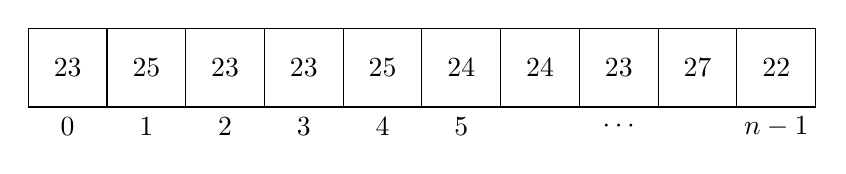
\begin{tikzpicture}
\filldraw [fill=white, draw=black] (0,0) rectangle (1,1) node[pos=.5] {23};
\filldraw [fill=white, draw=black] (1,0) rectangle (2,1) node[pos=.5] {25};
\filldraw [fill=white, draw=black] (2,0) rectangle (3,1) node[pos=.5] {23};
\filldraw [fill=white, draw=black] (3,0) rectangle (4,1) node[pos=.5] {23};
\filldraw [fill=white, draw=black] (4,0) rectangle (5,1) node[pos=.5] {25};
\filldraw [fill=white, draw=black] (5,0) rectangle (6,1) node[pos=.5] {24};
\filldraw [fill=white, draw=black] (6,0) rectangle (7,1) node[pos=.5] {24};
\filldraw [fill=white, draw=black] (7,0) rectangle (8,1) node[pos=.5] {23};
\filldraw [fill=white, draw=black] (8,0) rectangle (9,1) node[pos=.5] {27};
\filldraw [fill=white, draw=black] (9,0) rectangle (10,1) node[pos=.5] {22};
\node[] at (0.5,-0.25) {0};
\node[] at (1.5,-0.25) {1};
\node[] at (2.5,-0.25) {2};
\node[] at (3.5,-0.25) {3};
\node[] at (4.5,-0.25) {4};
\node[] at (5.5,-0.25) {5};
\node[] at (7.5,-0.25) {$\cdots$};
\node[] at (9.5,-0.25) {$n-1$};
\end{tikzpicture}
\end{center}
Il est important de remarquer que l'indice de la première case est 0 (et non 1 comme dans certains langages de programmation) et que celui de la
dernière case est $n-1$ (et non $n$). On a un accès direct à l'élément d'indice $k$ 
pour tout $k\in\interefo{0}{n}$ grâce à \verb!t[k]!. Si l'on tente d'accéder à un élément \verb!t[k]! pour $k\geq n$,
Python lève une exception qui se solde par une erreur.\\

Python permet aussi d'accéder aux éléments de la liste en les indexant \og par la fin \fg. On utilise
pour cela des indices strictement négatifs $k\in\interefo{-n}{0}$.
\begin{center}
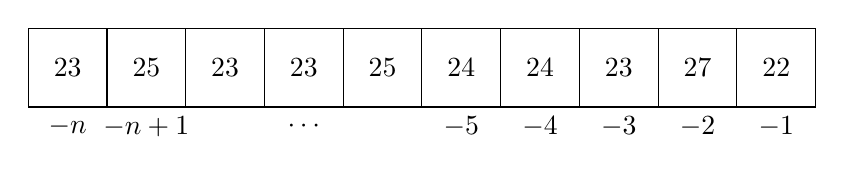
\begin{tikzpicture}
\filldraw [fill=white, draw=black] (0,0) rectangle (1,1) node[pos=.5] {23};
\filldraw [fill=white, draw=black] (1,0) rectangle (2,1) node[pos=.5] {25};
\filldraw [fill=white, draw=black] (2,0) rectangle (3,1) node[pos=.5] {23};
\filldraw [fill=white, draw=black] (3,0) rectangle (4,1) node[pos=.5] {23};
\filldraw [fill=white, draw=black] (4,0) rectangle (5,1) node[pos=.5] {25};
\filldraw [fill=white, draw=black] (5,0) rectangle (6,1) node[pos=.5] {24};
\filldraw [fill=white, draw=black] (6,0) rectangle (7,1) node[pos=.5] {24};
\filldraw [fill=white, draw=black] (7,0) rectangle (8,1) node[pos=.5] {23};
\filldraw [fill=white, draw=black] (8,0) rectangle (9,1) node[pos=.5] {27};
\filldraw [fill=white, draw=black] (9,0) rectangle (10,1) node[pos=.5] {22};
\node[] at (0.5,-0.25) {$-n$};
\node[] at (1.5,-0.25) {$-n+1$};
\node[] at (3.5,-0.25) {$\cdots$};
\node[] at (5.5,-0.25) {$-5$};
\node[] at (6.5,-0.25) {$-4$};
\node[] at (7.5,-0.25) {$-3$};
\node[] at (8.5,-0.25) {$-2$};
\node[] at (9.5,-0.25) {$-1$};
\end{tikzpicture}
\end{center}
Cependant, cette manière d'accéder aux listes est à priori proscrite aux concours. On se permettra
cependant d'utiliser la syntaxe bien pratique \verb!t[-1]! permettant d'accéder au dernier
élément d'une liste.\\

Les listes Python peuvent contenir des valeurs de types différents. Elles peuvent même contenir d'autres listes.

\begin{pythoncode}
In [2]: t = [9, 3.14159, "Hello", True, [3, 8]]
\end{pythoncode}

\noindent
Cependant, contrairement aux \verb_tuple_, l'utilisation des listes se fera essentiellement
avec des valeurs ayant le même type. Quels que soient les éléments qu'elle contient, le type d'une
liste est \verb!list!, mais dans la signature d'une fonction, on notera \verb!list['a]! pour désigner
le type d'une liste d'éléments de même type \verb!'a!.

\subsection{Parcours de liste}

Nous avons vu dans le second chapitre comment parcourir une liste. La manière la plus conventionnelle
est d'effectuer une boucle sur un entier $k$ qui va prendre successivement les indices admissibles
pour la liste. Par exemple, la fonction suivante va tester si un entier $x$ est un élément de la
liste $t$~:
\begin{pythoncodeline}
def est_present(x, t):
    """est_present(x: int, t: list[int]) -> bool"""
    for i in range(len(t)):
        if t[i] == x:
            return True
    return False
\end{pythoncodeline}
Il est cependant possible d'écrire la même fonction de manière plus concise, en itérant
non par sur les indices de la liste, mais directement sur la liste elle-même. Pour cela, on
utilise la syntaxe \og \verb!for y in t! \fg~: dans ce cas, la boucle va itérer sur les éléments
de la liste et $y$ va prendre successivement les valeurs $t_0, t_1,\ldots,t_{n-1}$. La fonction \verb!est_present! peut donc s'écrire ainsi~:
\begin{pythoncodeline}
def est_present(x, t):
    """est_present(x: int, t: list[int]) -> bool"""
    for y in t:
        if y == x:
            return True
    return False
\end{pythoncodeline}
Le fait qu'on puisse écrire \og \verb!for y in t! \fg fait de la liste \verb!t! un objet \emph{itérable}.
D'autres objets Python possèdent cette propriété~: les chaines de caractères et les tuples. La fonction
\verb!possede_un_e! vue au chapitre précédent s'écrit donc~:
\begin{pythoncodeline}
def possede_un_e(s):
    """possede_un_e(s: str) -> bool"""
    for c in s:
        if c == 'e':
            return True
    return False
\end{pythoncodeline}
Les deux styles ont chacun leurs avantages et leurs inconvénients. L'utilisation d'une liste en tant
qu'objet itérable a l'avantage de la concision, mais l'utilisation d'un indice et d'un \verb!range! est parfois nécessaire.\\

Nous avons vu dans le second chapitre des algorithmes de réduction permettant de
calculer la somme, le produit ou le maximum des éléments d'une liste. Ces algorithmes sont essentiels
et nous ne les redétaillerons pas ici. Nous allons plutôt détailler deux nouveaux algorithmes~:
l'algorithme de Horner et la méthode de recherche dichotomique dans une liste triée.

\subsubsection{Algorithme de Horner}

Les listes sont de bons candidats pour représenter les polynômes. Le polynôme 
$P\defeq p_0+p_1X+\cdots+p_n X^n$ sera ainsi représenté par la liste
$[p_0,p_1,\ldots,p_n]$ de longueur $n+1$. Si $x$ est un nombre, nous allons voir
différents algorithmes pour calculer $P(x)$. Si nous nous autorisons
l'exponentiation \verb!**!, nous obtenons une première
implémentation de cet algorithme~:
\begin{pythoncodeline}
def eval0(p, x):
    """eval0(p: list[int], x: int) -> int"""
    ans = 0
    for k in range(len(p)):
        ans = ans + p[k] * x**k
    return ans
\end{pythoncodeline}
Cependant, si on s'intéresse à la performance notre fonction, l'utilisation de \verb!**!
est problématique, car il n'existe pas d'instruction calculant la puissance d'un entier sur les
processeurs. Python va donc devoir générer du code dont nous n'avons pas le contrôle et dont
la performance est donc difficile à estimer. Si nous programmons nous-mêmes une
fonction naïve calculant $x^k$, nous obtenons l'implémentation suivante~:
\begin{pythoncodeline}
def puiss(x, n):
    """puiss(x: int, n: int) -> int"""
    ans = 1
    for _ in range(n):
        ans = ans * x
    return ans

def eval1(p, x):
    """eval1(p: list[int], x: int) -> int"""
    ans = 0
    for k in range(len(p)):
        ans = ans + p[k] * puiss(x, k)
    return ans
\end{pythoncodeline}
On peut s'intéresser au nombre de multiplications effectuées par notre algorithme. Le calcul
de $x^k$ par la fonction \verb!puiss! nécessite $k$ multiplications, donc le calcul de
\verb!p[k] * puiss(x, k)! nécessite $k+1$ multiplications, ce qui donne un cout de
\[C_1(n)\defeq \sum_{k=0}^n (k+1)=\frac{(n+1)(n+2)}{2}\]
multiplications. Il est possible de faire plus efficace en utilisant le fait qu'on a déjà calculé
$x^k$ lorsque l'on a besoin de calculer $x^{k+1}$. On utilise donc une variable \verb!xk! qui va accumuler le
produit des $x$ et contenir $x^k$.
\begin{pythoncodeline}
def eval2(p, x):
    """eval2(p: list[int], x: int) -> int"""
    ans = 0
    xk = 1
    for k in range(len(p)):
        ans = ans + p[k] * xk
        xk = xk * x
    return ans
\end{pythoncodeline}
Cet algorithme de nécessite que $C_2(n)\defeq 2(n+1)$ multiplications. Il est donc bien plus efficace
que notre premier algorithme puisque
\[\frac{C_2(n)}{C_1(n)}=\frac{4}{n+2}\tendvers{n}{+\infty}0.\]
Donc, plus $n$ devient grand, plus la différence de  performance entre les deux algorithmes va se
faire sentir.  On peut faire encore mieux en remarquant que
\begin{eqnarray*}
p_n x^n+p_{n-1}x^{n-1}+p_{n-2}x^{n-2}+\cdots+p_1 x+p_0
&=&(((p_n x+p_{n-1}) x+p_{n-2})x+\cdots+p_1)x+p_0\\
&=&((((0x + p_n) x+p_{n-1}) x+p_{n-2})x+\cdots+p_1)x+p_0.
\end{eqnarray*}
On aboutit à l'algorithme suivant, appelé algorithme de Horner
\begin{pythoncodeline}
def eval3(p, x):
    """eval3(p: list[int], x: int) -> int"""
    m = len(p)
    ans = 0
    for k in range(m):
        ans = ans * x + p[m - 1 - k]
    return ans
\end{pythoncodeline}
et qui nécessite seulement $C_3(n)\defeq n+1$ multiplications, soit deux fois moins que l'algorithme
précédent.

\subsubsection{Recherche dichotomique}

Nous avons vu plus haut comment effectuer une recherche linéaire dans une liste de longueur $n$ en
effectuant au plus $C_1(n)\defeq n$ comparaisons. Nous allons voir qu'il est possible de faire beaucoup plus efficace
lorsque cette liste est triée dans l'ordre croissant. Prenons l'exemple de la liste croissante
\verb!t = [1, 3, 7, 11, 12, 15, 19]!.
\begin{center}
\begin{tikzpicture}
\filldraw [fill=white, draw=black] (0,0) rectangle (1,1) node[pos=.5] {1};
\filldraw [fill=white, draw=black] (1,0) rectangle (2,1) node[pos=.5] {3};
\filldraw [fill=white, draw=black] (2,0) rectangle (3,1) node[pos=.5] {7};
\filldraw [fill=colorLazoBlue1Light, draw=black] (3,0) rectangle (4,1) node[pos=.5] {11};
\filldraw [fill=white, draw=black] (4,0) rectangle (5,1) node[pos=.5] {12};
\filldraw [fill=white, draw=black] (5,0) rectangle (6,1) node[pos=.5] {15};
\filldraw [fill=white, draw=black] (6,0) rectangle (7,1) node[pos=.5] {19};
\node[] at (0.5,-0.25) {0};
\node[] at (1.5,-0.25) {1};
\node[] at (2.5,-0.25) {2};
\node[] at (3.5,-0.25) {3};
\node[] at (4.5,-0.25) {4};
\node[] at (5.5,-0.25) {5};
\node[] at (6.5,-0.25) {6};
\end{tikzpicture}
\end{center}
Si nous cherchons l'élément $x$, on peut commencer à le comparer à $t_3=11$.
\begin{itemize}
\item Si $x=t_3$, il est présent dans la liste et l'algorithme se termine.
\item Si $x<t_3$, puisque la liste est triée dans l'ordre croissant, s'il est présent dans
  la liste, il est à gauche de 11. Il suffit donc de le chercher parmi les 3 premiers éléments.
  On va donc comparer $x$ à $t_1=3$ et on recommence notre procédé.
  \begin{center}
    \begin{tikzpicture}
    \filldraw [fill=white, draw=black] (0,0) rectangle (1,1) node[pos=.5] {1};
    \filldraw [fill=colorLazoBlue1Light, draw=black] (1,0) rectangle (2,1) node[pos=.5] {3};
    \filldraw [fill=white, draw=black] (2,0) rectangle (3,1) node[pos=.5] {7};
    \node[] at (0.5,-0.25) {0};
    \node[] at (1.5,-0.25) {1};
    \node[] at (2.5,-0.25) {2};
    \end{tikzpicture}
    \end{center}
  Soit $x$ va être égal à un moment à l'un des $t_k$ et le procédé se termine, soit notre sous-liste
  de travail devient vide ce qui prouve que $x$ ne fait pas partie de la liste initiale.
\end{itemize}
Pour implémenter notre algorithme, nous allons utiliser deux variables initialisées
à $g\defeq 0$ et $d\defeq n$ (la longueur de notre liste). À chaque itération, la tranche de recherche
 sera l'ensemble des éléments ayant un indice $k$ tel que $g\leq k<d$. On va considérer
l'indice $m \defeq \ent{(g+d)/2}$ et comparer $x$ à $t_m$.
\begin{center}
\begin{tikzpicture}
\filldraw [fill=white, draw=black] (0,0) rectangle (1,1) node[pos=.5] {1};
\filldraw [fill=white, draw=black] (1,0) rectangle (2,1) node[pos=.5] {3};
\filldraw [fill=white, draw=black] (2,0) rectangle (3,1) node[pos=.5] {7};
\filldraw [fill=colorLazoBlue1Light, draw=black] (3,0) rectangle (4,1) node[pos=.5] {11};
\filldraw [fill=white, draw=black] (4,0) rectangle (5,1) node[pos=.5] {12};
\filldraw [fill=white, draw=black] (5,0) rectangle (6,1) node[pos=.5] {15};
\filldraw [fill=white, draw=black] (6,0) rectangle (7,1) node[pos=.5] {19};
\node[] (A) at (0.5,-0.25) {0};
\node[] at (1.5,-0.25) {1};
\node[] at (2.5,-0.25) {2};
\node[] (E) at (3.5,-0.25) {};
\node[] at (4.5,-0.25) {$\cdots$};
\node[] at (6.5,-0.25) {$n-1$};
\node[] (C) at (7.5,-0.25) {$n$};

\node[] (B) at (0.5,-1.25) {$g$};
\node[] (D) at (7.5,-1.25) {$d$};
\node[] (F) at (3.5,-1.25) {$m$};
\draw[->] (B)--(A);
\draw[->] (D)--(C);
\draw[->] (F)--(E);
\end{tikzpicture}
\end{center}
\begin{itemize}
\item Si $x=t_m$, il est présent dans la liste et l'algorithme se termine.
\item Si $x<t_m$, on continue notre recherche dans la tranche $g\leq k < m$.
\item Si $x>t_m$, on continue notre recherche dans la tranche $m+1\leq k < d$.
\end{itemize}
Notre algorithme continue tant que la tranche de recherche est non vide, c'est-à-dire tant que $g<d$.

\begin{pythoncodeline}
def dichotomie(x, t):
    """dichotomie(x: int, t: list[int]) -> bool"""
    g = 0
    d = len(t)
    while g < d:
        m = (g + d) // 2
        if x == t[m]:
            return True
        elif x < t[m]:
            d = m
        else:              # Cas où x > t[m]
            g = m + 1
    return False
\end{pythoncodeline}
\noindent
Sur notre exemple possédant 7 éléments, l'algorithme de recherche linéaire nécessitait au plus 7 comparaisons alors
que la recherche dichotomique nécessite au plus 3 comparaisons. Plus généralement, on montre facilement
par récurrence que si $t$ possède $n\defeq 2^p-1$ éléments, la recherche dichotomique nécessite au plus
$p=\log_2(n+1)$ comparaisons. Sur un tableau de $1\ 023=2^{10}-1$ éléments, cela fait seulement 10 comparaisons
alors qu'une recherche linéaire peut en nécessiter $1\ 023$. On montrera dans le
chapitre sur la complexité que la recherche dichotomique
sur un tableau de taille $n$ quelconque nécessite au plus de l'ordre de $C_2(n)\defeq \log_2 n$ comparaisons.

\begin{exoUnique}
\exo Montrer que dans l'algorithme précédent, $d-g$ est un variant de boucle, et donc que l'algorithme
  termine.
\end{exoUnique}

\subsection{Création de liste}

Nous avons vu comment créer des listes contenant quelques éléments.  Si l'on souhaite
créer des listes plus grandes, diverses méthodes existent.

\subsubsection{Concaténation}
Comme pour les chaines de caractères, il est possible de concaténer deux listes.

\begin{pythoncode}
In [1]: [7, 2, 1] + [3, 5, 2]
Out[1]: [7, 2, 1, 3, 5, 2]
\end{pythoncode}

\noindent
On peut même multiplier des listes par un entier.

\begin{pythoncode}
In [2]: [1, 2, 3] * 3
Out[2]: [1, 2, 3, 1, 2, 3, 1, 2, 3]
\end{pythoncode}

\noindent
Cela nous sera notamment utile pour créer une liste formée de $n$ éléments identiques.

\begin{pythoncode}
In [3]: n = 10

In [4]: [0] * n
Out[4]: [0, 0, 0, 0, 0, 0, 0, 0, 0, 0]
\end{pythoncode}

\subsubsection{Compréhension}
Pour créer des listes plus complexes, on utilise ce qu'on appelle une \emph{compréhension}.

\begin{pythoncode}
In [1]: n = 5

In [2]: t = [k**2 for k in range(n)]

In [3]: t
Out[3]: [0, 1, 4, 9, 16]   
\end{pythoncode}
\noindent
Il est possible de créer des listes de listes en imbriquant des listes définies en compréhension.
\begin{pythoncode}
In [4]: [[10 * i + j for i in range(4)] for j in range(3)]
Out[4]: [[0, 10, 20, 30], [1, 11, 21, 31], [2, 12, 22, 32]]
\end{pythoncode}

Si l'on souhaite, on peut même ne garder que les éléments vérifiant une certaine condition. 
\begin{pythoncode}
In [5]: a = [k**2 for k in range(n) if k % 3 != 1]

In [6]: a
Out[6]: [0, 4, 9]  
\end{pythoncode}

% \begin{exoUnique}
% \exo  Un triplet pythagoricien est un triplet d'entiers $(x,y,z)\in\N^3$ tels que
%   $x^2+y^2=z^2$. Écrire une commande Python dont l'exécution renvoie la liste
%   des triplets pythagoriciens $(x,y,z)$ tels que $1\leq x\leq y\leq z < 20$.
% \begin{sol}
% \begin{pythoncode}
% [(x, y, z) for x in range(1, 20) for y in range(x, 20) for z in range(y, 20) if x**2 + y**2 == z**2]
% \end{pythoncode}
% \end{sol}
% \end{exoUnique}

\subsubsection{Slicing et copie}

Il est enfin possible de créer une nouvelle liste en dupliquant la tranche d'une liste déjà existante. On appelle
cette opération le \emph{slicing}.

\begin{pythoncode}
In [1]: t = [7, 1, 3, 9]

In [2]: a = t[1:3]

In [3]: a
Out[3]: [1, 3]
\end{pythoncode}

\noindent
Plus généralement, si $t$ est de longueur $n$ et $(i, j)\in\intere{0}{n}^2$ sont tels que $i\leq j$,
alors \verb_t[i:j]_ est la liste composée des objets $t_i, \ldots, t_{j-1}$. Lorsque l'indice
$i$ est omis, la valeur 0 est utilisée. Si
l'indice $j$ est omis, c'est la longueur de la liste qui est utilisée. On peut
aussi utiliser la forme plus avancée \verb!t[i:j:p]! où $p>0$ est le pas~:
cette tranche est alors formée des valeurs d'indices $i+kp$ pour $i\leq i+kp<j$.

\vspace{2ex}
\begin{exoUnique}
\exo Étant donné une liste \verb!t!, comment obtenir la liste de tous les éléments d'indices
  impairs~?
\end{exoUnique}
\vspace{2ex}

Si l'on souhaite faire une copie d'une liste \verb!t!, on peut
utiliser la syntaxe \verb!c = t[:]!. Nous verrons cependant plus tard
dans ce chapitre pourquoi cette technique fonctionne très bien pour
des listes de booléens, d'entiers ou de flottants mais pose problème
pour des listes de listes. Si l'on veut faire une copie de liste
de listes, le mieux est d'utiliser la
fonction \verb!deepcopy! du module \verb!copy!.

\begin{pythoncode}
In [4]: t = [[1, 2, 3], [4, 5, 6]]

In [5]: import copy

In [6]: c = copy.deepcopy(t)
\end{pythoncode}


\subsection{Modification des éléments}

Les éléments d'une liste sont accessibles en lecture et en écriture. Il est donc possible de changer leurs éléments.

\begin{pythoncode}
In [1]: note = [9, 10, 14]

In [2]: note[1] = 11

In [3]: note[2] = note[2] + 2

In [4]: note
Out[4]: [9, 11, 16]    
\end{pythoncode}
\noindent
Une liste de longueur $n$ se comporte donc comme $n$ variables avec lesquelles on peut
travailler. Supposons par exemple que l'on souhaite calculer les termes de la suite de Catalan
définie par
\[c_0\defeq 1\qsep \text{et}\quad \forall n\in\N\qsep c_{n+1}\defeq\sum_{k=0}^n c_{n-k}c_k.\]
Les premiers termes de cette suite sont $1, 1, 2, 5, 14, 42$, etc. Pour calculer le $n$-ième
terme de cette suite, on va créer un tableau $t$ de longueur $n+1$ dans lequel on va ranger
petit à petit les valeurs de $c_k$ pour $0\leq k\leq n$.

\begin{pythoncodeline}
def catalan(n):
    """catalan(n: int) -> int"""
    t = [None] * (n + 1)
    t[0] = 1
    for i in range(1, n + 1):
        c = 0
        for k in range(i):
            c = c + t[i - 1 - k] * t[k]
        t[i] = c
    return t[n]
\end{pythoncodeline}

\begin{exoUnique}
\exo Quel est le nombre de multiplications nécessaire au calcul de $c_n$~?
\end{exoUnique}

\vspace{2ex}
Nous savons que, grâce à la dichotomie, la recherche d'un élément dans une liste triée est
considérablement plus rapide que dans une liste quelconque. Nous avions cependant passé sous silence la manière dont
on peut trier une liste. De nombreux algorithmes sont dédiés à cette tâche. Les premiers que nous allons étudier
s'effectuent \og en place \fg, c'est-à-dire qu'ils fonctionnent en effectuant une succession d'échanges d'éléments.
Nous utiliserons pour cela la fonction
\begin{pythoncodeline}
def swap(t, i, j):
    """swap(t: list[int], i: int, j: int) -> NoneType"""
    t[i], t[j] = t[j], t[i]
\end{pythoncodeline}
\noindent
qui échange les éléments $t_i$ et $t_j$.

\subsubsection{Tri par sélection}

Le tri par sélection est le plus simple des algorithmes de tri et fonctionne de
la manière suivante~:
\begin{itemize}
\item On cherche d'abord l'élément le plus petit du tableau et on l'échange avec
  l'élément d'indice 0.
\item On cherche ensuite le plus petit élément d'indice $i\geq 1$ du tableau et
  on l'échange avec l'élément d'indice 1.
\end{itemize}
On continue ainsi jusqu'à la fin du tableau. Cet algorithme
est appelé \og tri par sélection\fg car il fonctionne en sélectionnant de
manière répétée le plus petit élément qui n'a pas encore été trié. Par exemple,
si on l'applique sur la liste \verb!t = [5, 1, 2, 6]!, on passe par les étapes
suivantes~: 

\begin{center}
\begin{tikzpicture}
\filldraw [fill=white, draw=black] (0,0) rectangle (1,1) node[pos=.5] {5};
\filldraw [fill=colorLazoPink2Light, draw=black] (1,0) rectangle (2,1) node[pos=.5] {1};
\filldraw [fill=white, draw=black] (2,0) rectangle (3,1) node[pos=.5] {2};
\filldraw [fill=white, draw=black] (3,0) rectangle (4,1) node[pos=.5] {6};

\filldraw [fill=colorLazoBlue1Light, draw=black] (0,-1.25) rectangle (1,-0.25) node[pos=.5] {1};
\filldraw [fill=white, draw=black] (1,-1.25) rectangle (2,-0.25) node[pos=.5] {5};
\filldraw [fill=colorLazoPink2Light, draw=black] (2,-1.25) rectangle (3,-0.25) node[pos=.5] {2};
\filldraw [fill=white, draw=black] (3,-1.25) rectangle (4,-0.25) node[pos=.5] {6};

\filldraw [fill=colorLazoBlue1Light, draw=black] (0,-2.5) rectangle (1,-1.5) node[pos=.5] {1};
\filldraw [fill=colorLazoBlue1Light, draw=black] (1,-2.5) rectangle (2,-1.5) node[pos=.5] {2};
\filldraw [fill=colorLazoPink2Light, draw=black] (2,-2.5) rectangle (3,-1.5) node[pos=.5] {5};
\filldraw [fill=white, draw=black] (3,-2.5) rectangle (4,-1.5) node[pos=.5] {6};

\filldraw [fill=colorLazoBlue1Light, draw=black] (0,-3.75) rectangle (1,-2.75) node[pos=.5] {1};
\filldraw [fill=colorLazoBlue1Light, draw=black] (1,-3.75) rectangle (2,-2.75) node[pos=.5] {2};
\filldraw [fill=colorLazoBlue1Light, draw=black] (2,-3.75) rectangle (3,-2.75) node[pos=.5] {5};
\filldraw [fill=white, draw=black] (3,-3.75) rectangle (4,-2.75) node[pos=.5] {6};
\end{tikzpicture}
\end{center}
\noindent
À chaque étape, les cases bleues représentent les éléments triés; ils sont donc à la bonne place dans notre tableau.
La case rose représente le plus petit élément parmi ceux qui ne sont pas encore triés. Afin de rendre notre
programme modulaire, on commence par écrire une fonction \verb!indice_minimum(t: list[int], i: int) -> int! qui
renvoie l'indice de l'élément le plus petit parmi les éléments $t_i,t_{i+1},\ldots,t_{n-1}$.

\begin{pythoncodeline}
def indice_minimum(t, i):
    """indice_minimum(t: list[int], i: int) -> int"""
    j_min = i
    for j in range(i + 1, len(t)):
        if t[j] < t[j_min]:
            j_min = j
    return j_min

def tri_selection(t):
    """tri_selection(t: list[int]) -> NoneType"""
    for i in range(len(t) - 1):
        j = indice_minimum(t, i)
        swap(t, i, j)
\end{pythoncodeline}

Si l'on souhaite calculer le nombre de comparaisons effectuées par cet algorithme, on constate que
pour tout $i$ tel que $0\leq i < n-1$, l'appel \verb!indice_minimum(t, i)! effectue $n-1-i$ comparaisons ligne 5. Cet algorithme effectue donc au total
\[C_s(n)\defeq (n-1)+(n-2)+\cdots+1 = \frac{n(n-1)}{2}\]
comparisons.\\

Le tri par sélection est une méthode de tri simple qui est facile à comprendre et
qui possède les propriétés suivantes~:
\begin{itemize}
\item \emph{Le nombre de comparaisons ne dépend que de la taille du tableau}. Cette
  propriété peut être à notre désavantage dans certaines situations. Par exemple,
  le temps d'exécution du tri par sélection sera le même sur un tableau déjà trié et
  sur un tableau de nombres aléatoires.
\item \emph{Le mouvement des données est minimal}. Chacune des boucles en $i$
  n'effectue qu'un échange d'éléments du tableau. Quelle que soit la liste à trier, il y a donc
  exactement $n-1$ échanges dans un tri par sélection.
\end{itemize}

\begin{exoUnique}
\exo Donner un invariant de la boucle présente ligne 11 prouvant que le tri par sélection
  effectue bien un tri de la liste $t$.
\end{exoUnique}

\subsubsection{Tri par insertion}

Le tri par insertion est l'algorithme que les gens utilisent généralement lorsqu'ils
veulent trier les cartes qu'ils ont en main. On insère chaque carte, de la gauche
vers la droite, dans la partie déjà triée qui se trouve sur la gauche.
Dans une implémentation informatique de cet algorithme, on a besoin d'insérer la carte
dans la partie déjà triée en effectuant des échanges successifs qui font remonter
petit à petit la carte à insérer à sa position.

\begin{center}
\includegraphics[width=0.7\textwidth]{../../commun/images/python-cours-insertion_carte}\\
Insertion de la carte 5 dans une main déjà triée
\end{center}
\noindent Par exemple,
si on l'applique sur la liste \verb!t = [5, 2, 1, 6]!, on passe par les étapes
suivantes~: 

\begin{center}
\begin{tikzpicture}
\filldraw [fill=colorLazoBlue1Light, draw=black] (0,0) rectangle (1,1) node[pos=.5] {5};
\filldraw [fill=colorLazoPink2Light, draw=black] (1,0) rectangle (2,1) node[pos=.5] {2};
\filldraw [fill=white, draw=black] (2,0) rectangle (3,1) node[pos=.5] {1};
\filldraw [fill=white, draw=black] (3,0) rectangle (4,1) node[pos=.5] {6};

\filldraw [fill=colorLazoBlue1Light, draw=black] (0,-1.25) rectangle (1,-0.25) node[pos=.5] {2};
\filldraw [fill=colorLazoBlue1Light, draw=black] (1,-1.25) rectangle (2,-0.25) node[pos=.5] {5};
\filldraw [fill=colorLazoPink2Light, draw=black] (2,-1.25) rectangle (3,-0.25) node[pos=.5] {1};
\filldraw [fill=white, draw=black] (3,-1.25) rectangle (4,-0.25) node[pos=.5] {6};

\filldraw [fill=colorLazoBlue1Light, draw=black] (0,-2.5) rectangle (1,-1.5) node[pos=.5] {1};
\filldraw [fill=colorLazoBlue1Light, draw=black] (1,-2.5) rectangle (2,-1.5) node[pos=.5] {2};
\filldraw [fill=colorLazoBlue1Light, draw=black] (2,-2.5) rectangle (3,-1.5) node[pos=.5] {5};
\filldraw [fill=colorLazoPink2Light, draw=black] (3,-2.5) rectangle (4,-1.5) node[pos=.5] {6};

\filldraw [fill=colorLazoBlue1Light, draw=black] (0,-3.75) rectangle (1,-2.75) node[pos=.5] {1};
\filldraw [fill=colorLazoBlue1Light, draw=black] (1,-3.75) rectangle (2,-2.75) node[pos=.5] {2};
\filldraw [fill=colorLazoBlue1Light, draw=black] (2,-3.75) rectangle (3,-2.75) node[pos=.5] {5};
\filldraw [fill=colorLazoBlue1Light, draw=black] (3,-3.75) rectangle (4,-2.75) node[pos=.5] {6};
\end{tikzpicture}
\end{center}
\indent À chaque étape, les cases bleues représentent la main triée et la case rose représente
la carte que l'on insère par échanges successifs dans notre main triée. Contrairement au tri par sélection,
les éléments bleus ne sont pas toujours dans leur position finale puisqu'il est possible
que ces éléments doivent plus tard faire place à des éléments plus petits qui seront insérés.

\begin{pythoncodeline}
def tri_insertion(t):
    """tri_insertion(t: list[int]) -> NoneType"""
    for i in range(1, len(t)):
        j = i - 1
        while j >= 0 and t[j] > t[j + 1]:
            swap(t, j, j + 1)
            j = j - 1
\end{pythoncodeline}
\noindent
Si l'on souhaite calculer le nombre de comparaisons effectuées par cet algorithme, on constate que
pour tout $i$ tel que $1\leq i<n$, la boucle de la ligne 6 effectue au plus $i$ comparaisons. Cet
algorithme effectue donc au total au plus
\[C_i(n) \leq 1+2+\cdots+(n-1)=\frac{n(n-1)}{2}\]
comparaisons. Contrairement au tri par sélection, ce nombre de comparaisons dépend non seulement de la taille de la liste, mais aussi de ses éléments.
\begin{itemize}
\item Si on effectue un tri par insertion sur une liste déjà triée, il effectue exactement $n-1$
  comparaisons.
\item Si on trie une liste triée dans l'ordre décroissant, on va effectuer
  exactement $n(n-1)/2$ comparaisons.
\end{itemize}
On peut démontrer qu'en moyenne, le tri par insertion effectue un nombre de comparaisons de l'ordre de $n^2/4$.\\

Le tri par insertion marche assez bien pour des tableaux qui ne sont pas aléatoires
et que l'on rencontre souvent en pratique. Pour des tableaux \og partiellement triés \fg, il
nécessite de l'ordre de $n$ comparaisons. Nous nous contenterons d'une idée assez floue de ce que
signifie ce terme; on peut dire cependant que les tableaux suivants sont partiellement triés~:
\begin{itemize}
\item Un petit tableau qui a été ajouté à la fin d'un gros tableau trié.
\item Un tableau avec seulement peu d'éléments qui ne sont pas au bon endroit.
\item Un tableau dont tous les éléments ne sont pas loin de leur position finale.
\end{itemize}
En résumé, le tri par insertion est une excellente méthode pour les tableaux qui
sont partiellement triés et pour les petits tableaux. Comme ces tableaux
arrivent dans des parties intermédiaires d'autres algorithmes de tri plus avancés,
nous le retrouverons dans des implémentations efficaces de tels algorithmes.



\subsection{Ajout et suppression d'éléments}

Si nous revenons à notre analogie où une liste fonctionne comme un porte-pantalon,
l'image suivante correspond à une liste de 3 éléments~:

\begin{center}
\includegraphics[width=0.3\textwidth]{../../commun/images/python-cours-jeans-tabdyn}
\end{center}
\noindent
Il est aisé d'ajouter un quatrième pantalon à côté du dernier. Les listes permettent
d'effectuer efficacement cette opération avec la méthode \verb!append!.

\begin{pythoncode}
In [1]: lst = [7, 2, 1]

In [2]: lst.append(5)

In [3]: lst
Out[3]: [7, 2, 1, 5]
\end{pythoncode}
\noindent
La syntaxe de cette fonction diffère de ce que nous avons vu pour le
moment. Cette syntaxe est héritée de ce qu'on appelle la \emph{programmation orientée objet} et c'est
la raison pour laquelle on parle de \emph{méthode} et non de \emph{fonction}. Cependant, la différence
entre ces deux notions sera purement syntaxique en prépa où nous n'étudierons pas la programmation
orientée objet~: il faut simplement imaginer que ce que nous écrivons \verb!lst.append(5)! aurait
pu s'écrire \verb!append(lst, 5)!.\\

Remarquons que les instructions \verb!t = t + [x]! et \verb!t.append(x)! ajoutent toutes les deux $x$ à la fin de 
$t$. Cependant, la première instruction crée une nouvelle liste alors que la seconde modifie la
liste déjà existante. Outre le fait qu'une modification de liste est bien plus efficace que la création
d'une nouvelle liste, ces deux opérations ne sont pas interchangeables.
En pratique, la première instruction n'est presque jamais utile et son utilisation doit être considérée avec
beaucoup de suspicion.\\

L'opération inverse, qui consiste à enlever le dernier élément d'une liste, est aussi disponible
grâce à la méthode \verb!pop!. Cette méthode agit de deux manières~:
\begin{itemize}
\item Elle fonctionne par effet de bord et enlève le dernier élément de la liste.
\item Elle renvoie la valeur de cet élément.
\end{itemize}
\begin{pythoncode}
In [4]: x = lst.pop()

In [5]: lst
Out[5]: [7, 2, 1]

In [6]: x
Out[6]: 5
\end{pythoncode}
Bien entendu, si la valeur de cet élément ne nous intéresse pas, il est possible d'appeler
\verb!lst.pop()! et d'ignorer la valeur renvoyée. Enfin, si la liste \verb!lst! est vide, un
appel à \verb!lst.pop()! va lever une exception et donc signaler une erreur.\\

Notons enfin l'existence d'une méthode \verb!extend! qui fonctionne de manière similaire
à la méthode \verb!append! mais qui ajoute tous les éléments d'une liste à la fin
d'une liste existente.
\begin{pythoncode}
In [7]: lst.extend([9, 3, 5])

In [8]: lst
Out[8]: [7, 2, 1, 9, 3, 5]
\end{pythoncode}
\vspace{2ex}

Afin de mettre en oeuvre la méthode \verb!append!,
supposons que l'on souhaite écrire une fonction qui renvoie la liste de tous
les nombres premiers inférieurs ou égaux à $n$. Nous remarquons que si $k\geq 2$ et si
nous avons la liste de tous les nombres premiers strictement inférieurs à $k$, il est
facile de savoir si $k$ est premier~: il suffit de voir si un des nombres premiers
dont on dispose divise $k$. Ce principe nous permet d'écrire l'algorithme suivant

\begin{pythoncodeline}
def admet_diviseur(n, t):
    """admet_diviseur(n: int, t: list[int]) -> bool"""
    for p in t:
        if n % p == 0:
            return True
    return False

def liste_premiers(n):
    """liste_premiers(n: int) -> list[int]"""
    lst = []
    for k in range(2, n + 1):
        if not admet_diviseur(k, lst):
            lst.append(k)
    return lst
\end{pythoncodeline}
\noindent On obtient ainsi
\begin{pythoncode}
In [9]: liste_premiers(20)
Out[9]: [2, 3, 5, 7, 11, 13, 17, 19]
\end{pythoncode}

\subsubsection{Tri fusion}

L'algorithme de tri que nous allons étudier dans cette section est basé sur une opération
simple appelée \emph{fusion}~: regrouper deux listes ordonnées en une liste
ordonnée plus grande. Cette opération conduit à une méthode de tri récursive 
de la famille \og diviser pour régner \fg appelée
tri fusion. Pour trier une liste, on divise la liste en deux parties, on
trie les deux parties de manière récursive et on fusionne les deux résultats.

\begin{center}
  \begin{tabular}{|r|c|c|c|c|c|c|c|c|}
  \hline
  entrée & 1 & 5 & 2 & 9 & 0 & 8 & 4 & 3\\
  moitié de gauche triée & \color{blue}1 & \color{blue}2 & \color{blue}5 & \color{blue}9 & \color{gray}0 & \color{gray}8 & \color{gray}4 & \color{gray}3\\
  moitié de droite triée & \color{gray}1 & \color{gray}2 & \color{gray}5 & \color{gray}9 & \color{red}0 & \color{red}3 & \color{red}4 & \color{red}8\\ 
  fusion & \color{red}0 & \color{blue}1 & \color{blue}2 & \color{red}3 & \color{red}4 & \color{blue}5 & \color{red}8 & \color{blue}9\\
  \hline
  \end{tabular}
  \end{center}
  
  Nous nous intéressons d'abord à l'algorithme de fusion.
  Pour cela, nous créons une liste vide à laquelle nous allons ajouter petit à petit les
  éléments des listes $t_1$ et $t_2$ par ordre croissant. Une fois qu'une des listes
  est épuisée, il suffit d'ajouter les éléments de l'autre liste.

\begin{pythoncodeline}
def fusion(t1, t2):
    """fusion(t1: list[int], t2: list[int]) -> list[int]"""
    t = []
    i1 = 0
    i2 = 0
    while i1 < len(t1) and i2 < len(t2):
        if t1[i1] < t2[i2]:
            t.append(t1[i1])
            i1 = i1 + 1
        else:
            t.append(t2[i2])
            i2 = i2 + 1
    t.extend(t1[i1:])
    t.extend(t2[i2:])
    return t
\end{pythoncodeline}

Une fois l'algorithme de fusion écrit, le tri fusion s'écrit facilement.
\begin{itemize}
\item \emph{cas de base}~: Si la liste est vide ou ne possède qu'un seul élément,
  elle est triée.
\item \emph{réduction}~: Si la liste est de de taille $n$, on la découpe en deux
  listes de tailles respectives $\ent{n/2}$ et $\ents{n/2}$. On trie ces listes
  de manière récursive que l'on fusionne ensuite.
\end{itemize}
On obtient alors l'implémentation suivante~:

\begin{pythoncodeline}
def tri_fusion(t):
    """tri_fusion(t: list[int]) -> list[int]"""
    n = len(t)
    if n <= 1:
        return t[:]
    n1 = n // 2
    t1 = tri_fusion(t[0:n1])
    t2 = tri_fusion(t[n1:n])
    t = fusion(t1, t2)
    return t
\end{pythoncodeline}
\noindent
Nous verrons dans le chapitre sur la complexité que l'algorithme de tri fusion utilise de l'ordre de $n\log n$ comparaisons.

\subsubsection{Tri rapide}

Le tri rapide est aussi un algorithme de la famille \og diviser pour régner \fg.
Il fonctionne en partitionnant le tableau en deux sous-tableaux et en triant ces
tableaux de manière indépendante. On commence par choisir au hasard un élément
de notre tableau qu'on appelle \emph{pivot} grâce à la fonction \verb!choice! du
module \verb!random!.
\begin{itemize}
\item On génère ensuite le tableau \verb!smaller! des éléments de $t$ qui sont
  strictement inférieurs au pivot.
\item De même, on génère le tableau \verb!equal! des éléments de $t$ qui sont
  égaux au pivot.
\item Enfin, on génère le tableau \verb!greater! des éléments de $t$ qui sont
  strictement supérieurs au pivot.
\end{itemize}
On trie ensuite de manière récursive les tableaux \verb!smaller! et \verb!greater!
avant de concaténer les tableaux obtenus.

\begin{pythoncodeline}
import random 

def quicksort(t):
    """quicksort(t: list[int]) -> list[int]"""
    if len(t) <= 1:
        return t[:]
    pivot = random.choice(t)
    smaller = [x for x in t if x < pivot]
    equal = [x for x in t if x == pivot]
    greater = [x for x in t if x > pivot]
    return quicksort(smaller) + equal + quicksort(greater)
\end{pythoncodeline}
\noindent
Nous verrons en exercice la \og vraie \fg version du tri rapide qui ne crée pas de tableau
auxiliaire mais s'effectue en place. Cette version effectue dans le pire des cas de l'ordre de $n^2/2$ comparaisons,
mais on peut montrer qu'en moyenne, elle effectue seulement de l'ordre de $n \log n$
comparaisons.

\subsection{Les objets Python}

Le lecteur attentif se sera peut-être rendu compte que les listes avaient un comportement étrange lorsqu'elles
étaient passées en argument d'une fonction. Pour mettre en valeur ce comportement, il peut être utile de
jouer avec les deux fonctions suivantes~:

\begin{pythoncodeline}
def f(n):
    """f(n: int) -> NoneType"""
    n = n + 1

def g(t):
    """g(n: list[int]) -> NoneType"""
    for k in range(len(t)):
        t[k] = t[k] + 1
\end{pythoncodeline}

\noindent Les deux essais suivants nous montrent bien que les entiers et les listes d'entiers réagissent
de manière différente.
\begin{pythoncode}
In [1]: a = 5

In [2]: f(a)

In [3]: a
Out[3]: 5
\end{pythoncode}

\begin{pythoncode}
In [4]: a = [5, 5, 5]

In [5]: g(a)

In [6]: a
Out[6]: [6, 6, 6]
\end{pythoncode}

\noindent 
Cette différence de comportement peut d'ailleurs s'observer sans fonction. Pour la comprendre,
nous avons besoin de revenir sur la notion d'\emph{objet} et de \emph{variable} en Python. L'idée même selon
laquelle une variable est une boite contenant une valeur va d'ailleurs être mise à mal~: c'était une
simplification de la réalité que les listes viennent de mettre en valeur.

\begin{pythoncode}
In [7]: a = [7, 2, 1]

In [8]: b = a

In [9]: a.append(5)

In [10]: a
Out[10]: [7, 2, 1, 5]

In [11]: b
Out[11]: [7, 2, 1, 5]
\end{pythoncode}
\noindent
Si les variables $a$ et $b$ étaient réellement des boites contenant des valeurs, une modification de $a$
n'aurait aucune influence sur $b$. Comme nous venons de voir sur cet exemple, ce n'est pas le cas. Pour
comprendre, ce phénomène, il est bon de détailler la notion d'objet.\\

En Python, toutes les données sont représentées par des objets, que ce soient des entiers, des nombres
flottants, des booléens, des chaines de caractères, des tuples, des listes et même des fonctions. Chaque
objet possède un identifiant, un type et une valeur~: on dit qu'en Python les valeurs sont \emph{boxées}.
\begin{itemize}
\item L'\emph{identifiant} d'un objet est l'adresse mémoire à laquelle il est stocké; on utilise aussi
  le nom de \emph{pointeur}. Il ne change pas au cours de la vie de l'objet et deux objets
  distincts ont des identifiants distincts. Nous verrons cependant que deux objets différents peuvent
  avoir la même valeur.
\item Le \emph{type} d'un objet est aussi une propriété qui ne change pas au cours de sa vie. Pour l'instant, nous
  avons vu essentiellement les types \verb!bool!, \verb!int!, \verb!float!, \verb!string!, \verb!tuple! et \verb!list!.
\item Enfin, un objet possède une \emph{valeur} qui peut changer où non au cours de sa vie, selon son type.
  Les valeurs des objets de type \verb_bool_, \verb_int_, \verb_float_, \verb_string_ et \verb!tuple! ne peuvent
  pas changer. On dit que ces types sont \emph{immuables}. Le seul moyen d'avoir une nouvelle valeur est de
  créer un nouvel objet. Contrairement aux autres, le type \verb!list! est \emph{mutable}~: les objets
  de type \verb!list! ont une valeur qui peut changer au cours de leur vie.
\end{itemize}

\vspace{2ex}
Comme nous l'avons observé, une variable n'est pas une boite dans laquelle on met une valeur.
C'est en fait une boite dans laquelle on met l'identifiant de l'objet auquel elle est associée. Par exemple,
l'instruction

\begin{pythoncode}
In [12]: a = 7
\end{pythoncode} 
\noindent
crée un objet de type \verb_int_ dont la valeur est 7 et associe la variable $a$ à cet objet.

\begin{center}
\includegraphics[width=0.25\textwidth]{../../commun/images/python-cours-tutor-1}
\end{center}

\noindent Lorsqu'on écrit ensuite

\begin{pythoncode}
In [13]: a = a + 1   
\end{pythoncode}
\noindent
Python crée un nouvel objet de type \verb_int_ dont la valeur est 8 et associe le nom $a$ à ce nouvel objet.

\begin{center}
\includegraphics[width=0.25\textwidth]{../../commun/images/python-cours-tutor-2}
\end{center}
\noindent
L'ancien objet de valeur 7 existe toujours, mais plus aucune variable ne pointe vers lui. Lors du prochain passage
du \emph{ramasse-miette} (\emph{garbage collector} en anglais), cet objet sera supprimé et la mémoire qu'il utilise
sera de nouveau disponible.\\

Nous pouvons maintenant comprendre pourquoi l'appel de la fonction $f$ définie plus haut n'a aucun effet sur
la variable $a$.

\begin{pythoncodeline}
def f(n):
    n = n + 1

a = 5
f(a)
\end{pythoncodeline}
Lorsqu'on est à la ligne 5 et qu'on appelle la fonction $f$, l'objet de valeur 5 est passé à la fonction
et une variable locale $n$ est créée.

\begin{center}
\includegraphics[width=0.25\textwidth]{../../commun/images/python-cours-tutor-4}
\end{center}
\noindent
L'instruction \verb!n = n + 1! de la ligne 2 crée un nouvel objet de valeur 6 vers lequel pointe la
variable $n$.
\begin{center}
\includegraphics[width=0.25\textwidth]{../../commun/images/python-cours-tutor-5}
\end{center}
\noindent
Lorsqu'on sort de la fonction, la variable $n$ est détruite et $a$ pointe toujours vers un objet
de valeur 5.\\

Le cas de la fonction $g$ est différent. 

\begin{pythoncodeline}
def g(t):
    for k in range(len(t)):
        t[k] = t[k] + 1

a = [5, 5, 5]
g(a)
\end{pythoncodeline}
\noindent
Lorsqu'on est à la ligne 6 et qu'on appelle la fonction $g$, l'objet de valeur \verb![5, 5, 5]! est passé
à la fonction et une variable locale $t$ est créée. Nous nous trouvons donc dans la situation où deux variables
pointent vers le même objet; ce phénomène est appelé \emph{aliasing}.
\begin{center}
\includegraphics[width=0.32\textwidth]{../../commun/images/python-cours-tutor-7}
\end{center}
\noindent
Contrairement à ce qui se passait dans le cas précédent où l'instruction \verb!n = n + 1! créait un nouvel
objet, l'instruction \verb!t[k] = t[k] + 1! fait muter la liste $t$ et l'on se retrouve dans l'état
suivant~:
\begin{center}
\includegraphics[width=0.32\textwidth]{../../commun/images/python-cours-tutor-8}
\end{center}
\noindent Lorsqu'on va sortir de la fonction, la variable $t$ sera détruite et $a$ pointera toujours vers
la liste qui a été modifiée par notre fonction.
\vspace{2ex}
\begin{exoUnique}
\exo À quelle valeur est associée $a$ après le script suivant~?
\begin{pythoncode}
a = [7, 2, 1]
b = a
b.append(5)
\end{pythoncode}
\end{exoUnique}
\vspace{2ex}

La réalité est encore plus complexe que cela. Comme nous l'avions dit, les cases d'une liste se
comportent comme des variables. Donc lorsqu'on écrit
\begin{pythoncodeline}
t = [7, 2, 1]
\end{pythoncodeline}
\noindent ce sont en fait les objets suivants qui sont créés.
\begin{center}
\includegraphics[width=0.35\textwidth]{../../commun/images/python-cours-tutor-10}
\end{center}
La représentation qui a été faite plus haut ne pose cependant aucun problème puisque les entiers sont
des valeurs immuables. Cependant, une telle représentation devient cruciale lorsqu'on commence à manipuler
des listes d'objets mutables, comme des listes de listes.
\begin{pythoncodeline}
t = [7, 2, 1]
a = [t, t]
t.append(5)
\end{pythoncodeline}
\noindent Juste avant l'exécution de la ligne 3, voici les relations entre les différents objets.
\begin{center}
\includegraphics[width=0.39\textwidth]{../../commun/images/python-cours-tutor-12}
\end{center}
Après ce script, $a$ va donc être associé à la valeur \verb![[7, 2, 1, 5], [7, 2, 1, 5]]!.
\vspace{2ex}
\begin{exoUnique}
\exo On souhaite créer une liste de $n$ listes. Si l'on écrit
\begin{pythoncodeline}
n = 3
a = [[]] * n
a[0].append(7)
\end{pythoncodeline}
  la liste $a$ va être associée à la valeur \verb![[7], [7], [7]]!. Cependant, si on écrit
\begin{pythoncodeline}
n = 3
a = [[] for _ in range(n)]
a[0].append(7)
\end{pythoncodeline}
la liste $a$ va être associée à la valeur \verb![[7], [], []]!. Dessiner dans les deux cas les différents objets
juste avant l'exécution de la $3^e$ ligne.
\end{exoUnique}
\vspace{2ex}
On retiendra de l'exercice précédent que si l'on souhaite créer une liste de $n$ zéros, l'expression
\verb![0] * n! fonctionne parfaitement, mais si l'on veut créer une liste de $n$ listes vides, il ne
faut surtout pas utiliser \verb![[]] * n! mais plutôt \verb![[] for _ in range(n)]!.\\

En résumé, on retiendra les points essentiels suivants~:
\begin{itemize}
\item En Python, les données sont représentées par des \emph{objets}.
\item Certains objets sont de types \emph{immuables}~: \verb_bool_, \verb_int_, \verb_float_, \verb_str_, \verb_tuple_.
  D'autres, comme \verb!list!, sont \emph{mutables}. Si une variable est associée à un objet d'un
  type immuable, on peut l'imaginer comme une boite contenant la valeur de cet objet.
  Cependant, si une variable est associée à un objet d'un type mutable, il est essentiel de se souvenir
  qu'elle pointe vers cet objet.
  Lorsque deux variables pointent vers un même objet, on dit qu'il y a \emph{aliasing}.
\item Une affectation \verb!a = expr! fait pointer \verb!a! vers l'objet en lequel \verb!expr! s'évalue.
  Si \verb!a! est associée à une liste, les instructions \verb!a.append(x)!, \verb!a.pop()! et
  \verb!a[k] = expr! font muter cette liste. Le slicing \verb!a[i:j]! crée une nouvelle liste
  dont les cases sont associées aux objets correspondants de la liste \verb!a!. On comprend maintenant pourquoi l'instruction \verb!c = t[:]! est
  à éviter lorsque \verb!t! est une liste de listes.
\item En Python, le passage des paramètres se fait \emph{par objet}~: à l'intérieur d'une fonction, les
  paramètres sont des variables locales associées aux objets passés lors de l'appel
  de la fonction. Si ces objets sont mutables, la fonction peut agir par effet de bord et changer
  leur valeur. Ces valeurs seront ensuite observables par l'appelant.
\end{itemize}

\vspace{2ex}
\begin{exoUnique}
\exo
\begin{questions}
\question Quelle est la valeur de \verb!a! après le script suivant~?
\begin{pythoncodeline}
a = [7, 2, 3, 5, 1]
b = a[1:4]
b[0] = b[0] + 1
\end{pythoncodeline}
\question Et après le script suivant~?
\begin{pythoncodeline}
a = [[7], [2], [3], [5], [1]]
b = a[1:4]
b[0].append(9)
\end{pythoncodeline}
\end{questions}
\end{exoUnique}


\section{Structures séquentielles}

\subsection{Pile}

Une \emph{pile} (\emph{stack} en anglais) est une structure de données linéaire qui se distingue par
ses conditions d'accès et d'ajout d'éléments~: c'est le principe du
\og dernier arrivé, premier servi\fg  (principe du \textsc{Lifo} pour Last In, First Out).
Un peu comme une pile d'assiettes, c'est la dernière assiette posée sur une pile
qui sera la première utilisée.

\begin{center}
\includegraphics[width=0.5\textwidth]{../../Commun/Images/python-cours-tableau-1.pdf}
\end{center}

Une réalisation concrète de cette structure de données fournit, outre la structure, les
fonctions suivantes~:
\begin{itemize}
\item Une fonction de création d'une pile vide.
\item Une fonction déterminant si une pile est vide.
\item Une fonction permettant d'empiler un élément au sommet de la pile.
\item Une fonction permettant de dépiler et de renvoyer l'élément au sommet d'une pile
  non vide.
\item Une fonction permettant de connaitre l'élément en haut d'une pile non vide.
\end{itemize}
La signature d'une pile d'entiers est donc la suivante~:
\begin{pythoncodeline}
stack_new() -> stack[int]
stack_is_empty(s: stack[int]) -> bool
stack_push(s: stack[int], x: int) -> NoneType
stack_pop(s: stack[int]) -> int
stack_peek(s: stack[int]) -> int
\end{pythoncodeline}

\begin{exos}
\exo Écrire une fonction \verb!trier(p: stack[int]) -> NoneType! qui prend en argument une pile $p$
  d'entiers et qui modifie l'ordre de ses éléments de sorte qu'en fin de traitement les
  nombres pairs soient placés sous les nombres impairs. On pourra pour ce faire créer et
  utiliser une ou plusieurs piles auxiliaires.
\begin{center}
\includegraphics[width=0.3\textwidth]{../../Commun/Images/python-exos-tableau-1.pdf}
\end{center}
\exo Expliquer comment implémenter une pile à l'aide d'une liste Python. On proposera une
  implémentation des 5 fonctions dont la spécification est donnée plus haut.
\end{exos}

\vspace{2ex}
Comme nous avons pu le voir dans l'exercice précédent, la structure de liste Python
est tellement bien adaptée à la structure de pile que lorsqu'on aura besoin d'une pile, on utilisera une
liste et on se limitera à l'usage des méthodes \verb!append!, \verb!pop! et à l'accès au dernier élément
par \verb!s[-1]!.


\subsection{File}

Une \emph{file} (\emph{queue} en anglais) est une structure de données linéaire fonctionnant
sur le principe du \textsc{Fifo} (First
In, First Out). On peut l'imaginer horizontale~: on rajoute des éléments par la droite
et on les enlève par la gauche. Cette fois, l'analogie se fait avec une file
d'attente. Les clients arrivent par la droite et la caisse est à gauche. Le prochain client
servi étant celui qui attend depuis le plus longtemps.

\begin{center}
  \includegraphics[width=0.6\textwidth]{../../commun/images/python-cours-file}
  \end{center}

% L'accession au poste de selectionneur
% de l'équipe de France de foot semble fonctionner selon une file de priorité que l'on pouvait
% représenter ainsi en 2010.

% \begin{center}
% \begin{tikzpicture}
% \filldraw [fill=white, draw=black] (0,0) rectangle (3,1) node[pos=.5] {Blanc};
% \filldraw [fill=white, draw=black] (3,0) rectangle (6,1) node[pos=.5] {Deschamps};
% % \filldraw [fill=white, draw=black] (6,0) rectangle (9,1) node[pos=.5] {Zidane};
% \node[] (A) at (-0.5,0.5) {};
% \node[] (B) at (-1.5,0.5) {};
% \draw[->] (A)--(B);
% \node[] (C) at (6.5,0.5) {};
% \node[] (D) at (7.5,0.5) {};
% \node[] at (10.5,0.5) {};
% \draw[->] (D)--(C);
% \end{tikzpicture}


% \begin{tikzpicture}
%   \filldraw [fill=white, draw=black] (0,0) rectangle (3,1) node[pos=.5] {Blanc};
%   \filldraw [fill=white, draw=black] (3,0) rectangle (6,1) node[pos=.5] {Deschamps};
%   % \filldraw [fill=white, draw=black] (6,0) rectangle (9,1) node[pos=.5] {Zidane};
%   \node[] (A) at (-0.5,0.5) {};
%   \node[] (B) at (-1.5,0.5) {};
%   \draw[->] (A)--(B);
%   \node[] (C) at (9.5,0.5) {};
%   \node[] (D) at (10.5,0.5) {};
%   \draw[->] (D)--(C);
%   \end{tikzpicture}
% \end{center}



Une réalisation concrète de cette structure fournit les
fonctions suivantes~:
\begin{itemize}
\item Une fonction de création d'une file vide.
\item Une fonction déterminant si un file est vide.
\item Une fonction permettant d'enfiler un élément à droite de la file.
\item Une fonction permettant de défiler et de renvoyer l'élément à gauche d'une file non vide.
\item Une fonction permettant de connaitre l'élément à gauche d'une file non vide.
\end{itemize}
La signature d'une file d'entiers est donc~:
\begin{pythoncodeline}
queue_new() -> queue[int]
queue_is_empty(q: queue[int]) -> bool
queue_push(q: queue[int], x: int) -> NoneType
queue_pop(q: queue[int]) -> int
queue_peek(q: queue[int]) -> int
\end{pythoncodeline}
\begin{exoUnique}
\exo Expliquer comment implémenter une file à l'aide d'une liste Python. On proposera une
  implémentation des 5 fonctions dont la spécification est donnée plus haut. Pourquoi cette
  implémentation est-elle inefficace~?
\end{exoUnique}

\vspace{2ex}
En pratique, on n'utilisera donc pas de liste Python lorsqu'on aura besoin d'une
file. On utilisera plutôt une \og double ended queue \fg ou \og deque \fg telle
qu'elle est disponible dans le module \verb!collections!.

\begin{pythoncodeline}
import collections

file = collections.deque() # Pour créer une file vide
n = len(file)              # Pour connaitre la longueur de la file
file.append(x)             # Pour enfiler un élément à droite
x = file.popleft()         # Pour défiler un élément à gauche
\end{pythoncodeline}

\subsection{File de priorité}

Une \emph{file de priorité} (\emph{priority queue} en anglais) est une structure de donnée linéaire où chaque élément de la file possède une priorité. Intuitivement, c'est avec une
telle structure de données que vous fonctionnez lorsqu'on vous donne du travail. 
Supposons que vous ayez plusieurs tâches à accomplir, listées par importance décroissante~:
travailler le cours de maths du jour, finir le DM de physique pour la
semaine prochaine et faire un gros score à flappy bird. On se représente cet ensemble de
tâches comme ceci
\begin{center}
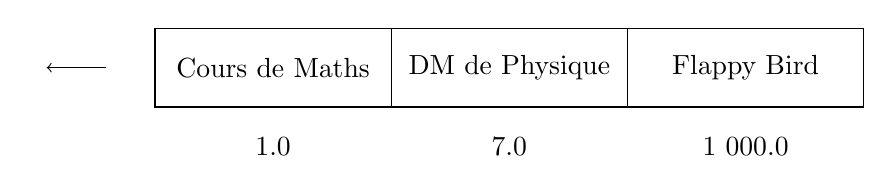
\begin{tikzpicture}
\filldraw [fill=white, draw=black] (0,0) rectangle (3,1) node[pos=.5] {Cours de Maths};
\filldraw [fill=white, draw=black] (3,0) rectangle (6,1) node[pos=.5] {DM de Physique};
\filldraw [fill=white, draw=black] (6,0) rectangle (9,1) node[pos=.5] {Flappy Bird};
\node[] at (1.5,-0.5) {1.0};
\node[] at (4.5,-0.5) {7.0};
\node[] at (7.5,-0.5) {$1\ 000.0$};
\node[] (A) at (-0.5,0.5) {};
\node[] (B) at (-1.5,0.5) {};
\draw[->] (A)--(B);
\end{tikzpicture}
\end{center}

\noindent
la flèche nous indiquant que la prochaine tâche à accomplir est de relire votre cours de
maths. Les nombres flottants placés en dessous de chaque tâche sont des priorités~: plus ce nombre
est bas, plus la tâche est prioritaire. Si vous apprenez que votre prochaine colle de
français a lieu dans trois jours, il faut vous ménager du temps
pour la préparer. Vous insérez donc cette nouvelle tâche dans la file avec une
priorité de $3.0$.  

\begin{center}
\begin{tikzpicture}
\filldraw [fill=white, draw=black] (0,0) rectangle (3,1) node[pos=.5] {Cours de Maths};
\filldraw [fill=colorLazoBlue1Light, draw=black] (3,0) rectangle (6,1) node[pos=.5] {Colle de Français};
\filldraw [fill=white, draw=black] (6,0) rectangle (9,1) node[pos=.5] {DM de Physique};
\filldraw [fill=white, draw=black] (9,0) rectangle (12,1) node[pos=.5] {Flappy Bird};
\node[] at (1.5,-0.5) {1.0};
\node[] at (4.5,-0.5) {3.0};
\node[] at (7.5,-0.5) {7.0};
\node[] at (10.5,-0.5) {$1\ 000.0$};
\node[] (A) at (-0.5,0.5) {};
\node[] (B) at (-1.5,0.5) {};
\draw[->] (A)--(B);
\end{tikzpicture}
\end{center}
Une réalisation concrète d'une file de priorité fournit donc les
fonctions suivantes~:
\begin{itemize}
\item Une fonction de création d'une file de priorité vide.
\item Une fonction déterminant si une file de priorité est vide.
\item Une fonction permettant d'enfiler un élément, accompagné d'une priorité.
\item Une fonction permettant de défiler l'élément ayant la priorité la plus basse.
\item Une fonction permettant de connaitre l'élément ayant la priorité la plus basse.
\end{itemize}
La signature d'une file de priorité d'entiers est donc~:

\begin{pythoncodeline}
pqueue_new() -> pqueue[int]
pqueue_is_empty(q: pqueue[int]) -> bool
pqueue_push(q: pqueue[int], x: int, p: float) -> NoneType
pqueue_pop(q: pqueue[int]) -> tuple[int, float]
pqueue_peek(q: pqueue[int]) -> tuple[int, float]
\end{pythoncodeline}

\begin{exoUnique}
\exo Expliquer comment implémenter une file de priorité d'entiers à l'aide d'une liste
  du tuples composés d'un entier et d'un nombre flottant.
\end{exoUnique}

\vspace{2ex}
Cette implémentation est cependant loin d'être efficace. Lorsque nous aurons besoin
d'une meilleure efficacité, nous pourrons utiliser le module \verb!heapq!.

\begin{pythoncodeline}
import heapq

filep = []                    # Pour créer une file de priorité vide
n = len(filep)                # Pour connaitre la longueur de la file
heapq.heappush(filep, (p, x)) # Pour insérer un élément x de priorité p
p, x = heapq.heappop(filep)   # Pour défiler un élément de priorité minimale
\end{pythoncodeline}

\subsection{Dictionnaire}

Un \emph{dictionnaire} présente de nombreuses similitudes avec les listes, si ce n'est qu'au lieu d'accéder aux éléments
par le biais d'un indice, on y accède par le biais d'une \emph{clé}. On crée un dictionnaire en suivant la
syntaxe \verb!{c1: v1, ..., cn: vn}! où $c_1,\ldots,c_n$ sont des clés, nécessairement deux à deux
distinctes, et $v_1,\ldots,v_n$ les valeurs qui leur sont associées. Ainsi, \verb!{}! crée un dictionnaire
vide.

\begin{pythoncode}
In [1]: prof = {"Info": "Fayard", "Maths": "Fayard", "Physique": "Villegas"}

In [2]: prof["Maths"]
Out[2]: 'Fayard'
\end{pythoncode}

Si $d$ est un dictionnaire et $c$ est une clé~:
\begin{itemize}
\item L'expression \verb!c in d! renvoie un booléen indiquant si la clé $c$ est présente dans le dictionnaire.
\item L'expression \verb!d[c]! renvoie la valeur associée à la clé si celle-ci est présente dans le dictionnaire.
\item L'instruction \verb!d[c] = v! crée une nouvelle association si la clé n'est pas présente dans le
  dictionnaire, et modifie l'association précédente sinon.
\item L'instruction \verb!del d[c]! supprime l'entrée associée à la clé $c$ dans le dictionnaire.
\item On peut enfin connaitre le nombre de clés présentes dans un
  dictionnaire avec la fonction \verb!len(d)!.
\end{itemize}

Le type d'un dictionnaire est \verb!dict!. En pratique les clés seront toutes d'un même type et les valeurs
seront aussi toutes du même type. Dans la signature des fonctions, on notera \verb!dict[str, int]! un dictionnaire
dont les clés sont des chaines de caractères et les valeurs sont des entiers.\\

Il est possible d'itérer sur les clés d'un dictionnaire avec la construction
\verb!for k in d.keys()!, mais on peut aussi directement itérer sur les clés et les
valeurs avec la construction \verb!for k, v in d.items()!. Par exemple~:
\begin{pythoncode}
In [3]: for k, v in prof.items():
   ...:     print("Le cours de", k, "est enseigné par M.",  v)
(*@\textcolor{purple}{Le cours de Info est enseigné par M. Fayard}@*)
(*@\textcolor{purple}{Le cours de Maths est enseigné par M. Fayard}@*)
(*@\textcolor{purple}{Le cours de Physique est enseigné par M. Villegas}@*)
\end{pythoncode}
Ces deux méthodes sont celles préconisées par le programme de prépa, mais il est plus naturel
en Python d'utiliser directement \verb!for k in d! qui a le même effet que
\verb!for k in d.keys()!. Le même programme s'écrit alors~:
\begin{pythoncode}
In [4]: for k in prof:
   ...:     print("Le cours de", k, "est enseigné par M.",  prof[k])
\end{pythoncode}
\vspace{2ex}
\begin{exoUnique}
\exo Écrire une fonction \verb!occ(lst: list[str]) -> dict[str, int]! renvoyant un dictionnaire \verb!d! tel
  que si \verb!s! est une chaine de caractères, \verb!d[s]! est le nombre d'occurrences de \verb!s! dans la liste
  \verb!lst!.
\end{exoUnique}
\vspace{2ex}
Il est possible de simuler un ensemble à l'aide d'un dictionnaire. Un ensemble d'entiers \verb!s! sera tout
simplement un dictionnaire \verb!dict[int, NoneType]!. On ajoutera un entier \verb!a! à cet ensemble
à l'aide de l'instruction \verb!s[a] = None! et on le supprimera avec l'instruction
\verb!del s[a]!.



%END_BOOK

\end{document}

% \section{Exercices}
% \setcounter{numeroexercice}{1}
% \input{exos-liste_pile_file}

\chapter{Représentation des données}
\setcounter{numeroexercicecours}{1}
\documentclass{magnolia}

\magtex{tex_driver={pdftex},
        tex_packages={xypic}}
\magfiche{document_nom={Cours Python sur la mémoire},
          auteur_nom={François Fayard},
          auteur_mail={fayard.prof@gmail.com}}
\magcours{cours_matiere={python},
          cours_niveau={mpsi},
          cours_chapitre_numero={5},
          cours_chapitre={Représentation des données}}
\magmisenpage{}
\maglieudiff{}
\magprocess

%\usepackage{minted}
%\usemintedstyle{xcode}

\begin{document}
%BEGIN_BOOK
\hfill\includegraphics[width=0.25\textwidth]{../../Commun/Images/python-cours-sudoku.jpg}
\magtoc

% quantité mémoire
% integrale

\vspace{2ex}
Un ordinateur possède une mémoire vive, appelée \textsc{Ram} pour \og Random Access
Memory\fg. C'est cette mémoire qui matérialise l'état du système. Concrètement, les
barrettes mémoire contiennent des milliards de condensateurs qui peuvent être
chargés ou déchargés. Lorsqu'un condensateur est chargé, il représente le \emph{bit} 1. S'il est déchargé,
il représente le bit 0.

\begin{center}
\begin{tabular}{|l||c|c|c|c|c|c|c|c|c|c|c|c|}
\hline
condensateur & 0 & 1 & 2 & 3 & 4 & 5 & 6 & 7 & 8 & 9 & 10 & $\ldots$ \\
\hline
état & 0 & 1 & 0 & 0 & 1 & 0 & 1 & 1 & 0 & 0 & 1 & $\ldots$ \\
\hline
\end{tabular}
\end{center}
\noindent
Une succession de 8 bits est appelée un \emph{octet}~: c'est la plus petite quantité
de mémoire adressable par un ordinateur. Les quantités de mémoire se comptent
en kilooctets ($1\ 000\approx 2^{10}$ octets), mégaoctets ($10^6\approx 2^{20}$ octets),
gigaoctets ($10^9\approx 2^{30}$ octets) et téraoctets ($10^{12}\approx 2^{40}$ octets).\\

Dans ce chapitre, nous allons voir comment une succession de 0 et de 1 peut être
utilisée pour représenter des entiers et des nombres flottants.

\section{Les entiers}

\subsection{Décomposition en base $b$}
% \subsection{Décomposition en base $b$}

L'écriture de l'entier 1984 décrit un nombre formé de 4 unités, 8 dizaines, 9 centaines
et 1 millier~:
\[1984 = 4\times 10^0 +\ 8\times 10^1 + \ 9 \times 10^2 + \ 1\times 10^3.\]
Le choix de faire des paquets en utilisant des puissances de 10 est cependant arbitraire.
On peut tout aussi bien décider d'utiliser des puissances de 2, 12, 16 ou 60. Si l'on choisit
d'utiliser des puissances de $b$, on dit qu'on décompose notre nombre en base $b$.

\begin{proposition}
Soit $b\geq 2$ un entier et $w\in\N$. Alors, pour tout $n\in\interefo{0}{b^w}$, il existe un unique $w$-uplet $(d_0,d_1,\ldots,d_{w-1})$ d'éléments de $\interefo{0}{b}$ tel que
\[n=\sum_{k=0}^{w-1} d_k b^k.\]
\end{proposition}

\begin{preuve}
Nous allons prouver ce résultat par récurrence sur $n$. Soit $b\geq 2$ un entier. Pour tout $n\in\N$, on pose
\begin{center}
$\mathcal{H}_n\defeq$ \og
\begin{minipage}[t]{0.6\linewidth}
Quel que soit $m\in\interefo{0}{b^n}$, il existe un unique $n$-uplet $(d_0,d_1,\ldots,d_{n-1})$ d'éléments de $\interefo{0}{b}$ tel que
$m=\sum_{k=0}^{n-1} d_k b^k$.\fg
\end{minipage}
\end{center}
\begin{itemize}
\item \emph{$\mathcal{H}_0$ est vraie}~: En effet, si $m\in\interefo{0}{1}$, alors $m=0$. Puisque qu'il existe un unique $0$-uplet d'éléments de $\interefo{0}{1}$ et qu'une somme vide est égale à 0, $\mathcal{H}_0$ est prouvée.
\item $\mathcal{H}_n\implique\mathcal{H}_{n+1}$~: Soit $n\in\N$. On suppose que $\mathcal{H}_n$ est vraie. Montrons que $\mathcal{H}_{n+1}$ est vraie. Soit $m\in\interefo{0}{b^{n+1}}$ et montrons qu'il existe un unique $(n+1)$-uplet $(d_0,\ldots,d_n)$ d'éléments de $\interefo{0}{b}$ tel que
\[m=\sum_{k=0}^{n} d_k b^k.\]
\begin{itemize}
\item \emph{Existence~:} On effectue la division euclidienne de $m$ par $b$. Il existe donc $q\in\N$ et $d_0\in\interefo{0}{b}$ tels que $m=qb+d_0$. Puisque $qb+d_0< b^{n+1}$, on en déduit que $qb<b^{n+1}$, puis que $q<b^n$. Puisque $\mathcal{H}_n$ est vraie, il existe donc un $n$-uplet $(d_1,\ldots,d_n)$ d'éléments de $\interefo{0}{b}$ tels que $q=\sum_{k=0}^{n-1} d_{k+1} b^k$. Alors
\begin{eqnarray*}
m & = & d_0+\p{\sum_{k=0}^{n-1} d_{k+1} b^k}b = d_0+\sum_{k=0}^{n-1} d_{k+1} b^{k+1}\\
  & = & d_0+\sum_{k=1}^{n} d_{k} b^{k} = \sum_{k=0}^{n} d_{k} b^{k}.
\end{eqnarray*}
\item \emph{Unicité~:} Soit $(d_0,\ldots,d_n)$ et $(e_0,\ldots,e_n)$ deux $(n+1)$-uplets d'éléments de $\interefo{0}{b}$ tels que
\[m=\sum_{k=0}^n d_k b^k \quad\et\quad m=\sum_{k=0}^n e_k b^k.\]
Montrons que pour tout $k\in\intere{0}{n}$, $d_k=e_k$. On a
\[m=\sum_{k=0}^{n} d_{k} b^{k} = \underbrace{\p{\sum_{k=1}^n d_k b^{k-1}}}_{\in\Z}b + \underbrace{d_0}_{\in\interefo{0}{b}}\]
donc $d_0$ est le reste de la division euclidienne de $m$ par $b$. De même, $e_0$ est le reste de la division euclidienne de $m$ par $b$. Par unicité du reste de la division euclidienne, on en déduit que $d_0=e_0$. De même, par unicité du quotient de la division euclidienne, on en déduit que
\[\sum_{k=1}^n d_k b^{k-1}=\sum_{k=1}^n e_k b^{k-1},\]
ce qui donne, après réindexation
\[\sum_{k=0}^{n-1} d_{k+1} b^k=\sum_{k=0}^{n-1} e_{k+1} b^k.\]
On pose alors $m'\defeq \sum_{k=0}^{n-1} d_{k+1} b^k$. Puisque $0\leq d_{k+1}\leq b-1$ pour tout $k\in\intere{0}{n-1}$, on en déduit que
\[0\leq m' \leq \sum_{k=0}^{n-1} (b-1)b^k=(b-1)\sum_{k=0}^{n-1} b^k=(b-1)\frac{1-b^n}{1-b}=b^n-1.\]
Puisque $\mathcal{H}_n$ est vraie, on en déduit que pour tout $k\in\intere{1}{n}$, $d_k=e_k$, ce qui finit de prouver l'unicité.
\end{itemize}
On a donc prouvé que $\mathcal{H}_{n+1}$ est vraie.
\end{itemize}
Par récurrence sur $n$, on en déduit que $\mathcal{H}_n$ est vraie pour tout $n\in\N$.
\end{preuve}

\begin{remarques}
\remarque On parle de \emph{décomposition en base $b$} de l'entier $n$. Les $d_k$ sont appelés
  \emph{chiffres} de $n$ en base $b$.
\remarque Les chiffres correspondant aux plus grandes puissances de $b$ sont dits
    \emph{plus significatifs} ou de \emph{poids fort}. Ceux qui correspondent aux
    petites puissances de $b$ sont dits \emph{moins significatifs} ou de
    \emph{poids faible}.
\remarque Pour tout $n\in\Ns$, il existe un unique $w\in\Ns$ et un unique
  $w$-uplet $(d_0,d_1,\ldots,d_{w-1})$ d'éléments de $\interefo{0}{b}$ tel que
  $d_{w-1}\neq 0$ et $n=\sum_{k=0}^{w-1} d_k b^k$. On écrit
  \[n=\underline{d_{w-1}\cdots d_1 d_0}_{b}.\]
  Lorsqu'on parle de \emph{la} décomposition de $n$ en base $b$, c'est de cette écriture
  qu'il s'agit. 
  Par exemple $13=\underline{13}_{10}$ car $13=3\times 10^0 + 1\times 10^1$ et
  $13=\underline{1101}_{2}$ car $13=1\times 2^0+0\times 2^1+1\times 2^2+1\times 2^3$. Par convention, la décomposition de 0 est vide, quelle que soit la base.
\remarque En base 2, les valeurs possibles pour un chiffre sont $0$ et $1$; on
  parlera indifféremment de \emph{bit} ou de chiffre. Étant donné l'importance de la
  base 2 en informatique, il est bon de connaitre les premières puissances de 2.
  \[\begin{array}{|c|c|c|c|c|c|c|c|c|c|c|}
  \hline
  \raisebox{10pt}{} 2^0 & 2^1 & 2^2 & 2^3 & 2^4 & 2^5 & 2^6 & 2^7 & 2^8 & 2^9 & 2^{10} \\
  \hline
  \raisebox{10pt}{} 1 & 2 & 4 & 8 & 16 & 32 & 64 & 128 & 256 & 512 & 1\ 024 \\
  \hline
  \end{array}\]
\remarque Si la base est supérieure à dix, on a un problème pour l'écriture~: il y a moins
  de chiffres usuels que de chiffres de la base. Le seul cas que l'on rencontre en pratique
  est celui de la base 16 dite \emph{hexadécimale}. La convention est d'utiliser les lettres
  de \verb!A! à \verb!F! pour représenter les chiffres de 10 à 15. 
\remarque Les bases 2, 16 et dans une moindre mesure 8, sont couramment utilisées
  en informatique. Par conséquent, il est possible d'écrire les littéraux directement dans
  ces bases. En Python, la syntaxe est~:
\begin{pythoncode}
In [1]: 0b10010
Out[1]: 18

In [2]: 0xff
Out[2]: 255

In [3]: 0o77
Out[3]: 63
\end{pythoncode}
\remarque Si l'on veut obtenir les chiffres de 137 en base 10, on commence par écrire
  que $137 = 13 \times 10 + 7$~: on effectue la division euclidienne de 137 par 10.
  Le chiffre de poids faible $d_0$ est donc $7$, et avant cela on a les chiffres de 13. 
  De même, $13 = 1 \times 10 + 3$, donc $d_1 = 3$, et on continue en remplaçant $13$ par 1. Enfin
  $1 = 0 \times 10 + 1$, donc $d_2 = 1$. On remplace $1$ par $0$ et on a terminé car $0$
  n'a «~pas de chiffre~». On a donc $137 = \underline{137}_{10}$.
\remarque Si au contraire on dispose de la liste des chiffres en base $b$ et que l'on
  souhaite obtenir $n$, le plus efficace est de remarquer  que
  \[\sum_{k = 0}^{w-1} d_k b^k
  = d_0 + b\p{d_1 + b\p{d_2 + \cdots b \p{d_{w-2} + b d_{w-1}}}}.\]
  Cette écriture est à la base de l'algorithme de Horner~: on part de 0 et on
  multiplie successivement notre valeur par 10 avant de lui ajouter $d_k$, pour toutes
  les valeurs de $k$ allant en décroissant de $w-1$ à $0$. Si l'on souhaite
  calculer $\underline{137}_{10}$, on effectue donc les calculs
  \[
    0 \xrightarrow[\times 10+1]{}  1
    \xrightarrow[\times 10+3]{}  13
    \xrightarrow[\times 10+7]{} 137.
  \]
\end{remarques}

\begin{exos}
  \exo Calculer $\underline{1000110}_2$ et $\underline{C7}_{16}$.
  \exo Donner l'écriture binaire de 59 et de 31. Quel phénomène général peut-on
    remarquer dans le deuxième cas ?
  \exo Comment s'écrit $\underline{102}_3$ en base 5 ?
\end{exos}
\vspace{2ex}
La fonction \verb!eval_lsd(b: int, d: list[int]) -> int! (\verb!lsd! pour
  least significant digit)
  renvoie l'entier dont l'écriture en base $b$ est \[\underline{d_{w - 1}\dots d_{0}}_{b}\]
  en utilisant l'algorithme de Horner.
\begin{pythoncodeline}
def eval_lsd(b, d):
    """eval_lsd(b: int, d: list[int]) -> int"""
    w = len(d)
    n = 0
    for k in range(w):
        n = n * b + d[w - 1 - k]
    return n
\end{pythoncodeline}

La fonction \verb!digits_lsd(b: int, n: int) -> list[int]!
  renvoie la liste des chiffres de $n$ en base $b$, le chiffre le moins significatif étant en premier.
\begin{pythoncodeline}
def digits_lsd(b, n):
    """digits_lsd(b: int, n: int) -> list[int]"""
    d = []
    while n > 0:
        d.append(n % b)
        n = n // b
    return d
\end{pythoncodeline}
Ces deux fonctions sont bien entendu à connaitre sur le bout des doigts.\\


\begin{proposition}
  Soit $b \geq 2$ un entier. Un entier $n > 0$ s'écrit avec $w=1 + \lfloor \log_b (n) \rfloor$ chiffres
    en base $b$.
  \end{proposition}

\vspace{2ex}
Les opérations d'addition et de multiplication apprises à l'école primaire fonctionnent
tout aussi bien en base $b\geq 2$ qu'en base 10. Entrainez-vous avec les exercices suivants pour
vous convaincre de cela.
\vspace{2ex}
\begin{exos}
\exo Effectuer l'addition $\underline{100110}_2 + \underline{1011}_2$
  en base 2, c'est-à-dire sans jamais convertir un nombre en base 10.
\exo Effectuer la multiplication $\underline{100110}_2 \times \underline{1011}_2$
  en base 2.
\exo Écrire les tables de multiplication en base 3. Calculer
  le produit $\underline{1022}_3 \times \underline{221}_3$ en travaillant en base 3.
\end{exos}
\vspace{2ex}
La décomposition en base 2 nous permet de revenir sur l'algorithme d'exponentiation
rapide dont nous avons donné une version récursive dans le chapitre sur les fonctions et
dont nous donnons ici une version itérative. Étant donné $n\in\N$, on effectue
sa décomposition en base 2
\[n=\sum_{k=0}^{w-1} d_k 2^k\]
et on remarque que pour tout $x$
\[x^n=x^{\sum_{k=0}^{w-1} d_k 2^k}=\prod_{k=0}^{w-1} \cro{x^{\p{2^k}}}^{d_k}.\]
Comme $d_k\in\ens{0,1}$, quel que soit $k\in\intere{0}{w-1}$, le terme entre crochets
est soit présent dans le produit (si $d_k=1$) soit absent (si $d_k=0$). De plus, il est aisé de calculer les
valeurs successives de $x^{2^k}$ car chaque terme est le carré du précédent.
On obtient ainsi l'algorithme d'exponentation rapide dans sa version itérative.

\begin{pythoncodeline}
def expo(x, n):
    """expo(x: int, n: int) -> int"""
    ans = 1
    y = x
    m = n
    while m > 0:
        if m % 2 == 1:
            ans = ans * y
        y = y * y
        m = m // 2
    return ans
\end{pythoncodeline}

\subsection{Représentation mémoire des entiers non signés}

La décomposition en base 2 nous donne un moyen de représenter les nombres positifs
à l'aide d'une séquence de bits.  Comme cette décomposition s'effectue uniquement pour
les entiers positifs, on parle de représentation des entiers \emph{non signés}. C'est cette
représentation que les processeurs utilisent pour manipuler les entiers non signés. Il ne sont
cependant capables que de travailler avec des entiers ayant une largeur $w$ fixée.
Aujourd'hui, un processeur 64~bits peut travailler avec des entiers codés sur 8, 16, 32
ou 64 bits.

\begin{proposition}
Pour une largeur de $w\in\N$, le plus grand entier non signé représentable est $2^{w} - 1$.
\end{proposition}

Avec 8 bits, on peut coder tous les entiers entre 0 et $2^8-1=255$. 
Avec 16 bits, on peut coder tous les entiers entre 0 et $2^{16}-1=65\ 535$.
Avec 32 bits on peut coder
tous les entiers entre 0 et $2^{32}-1=4\,294\,967\,295$, soit quelques milliards. Avec
64 bits on peut coder tous les entiers entre 0 et quelques milliards de milliards, ce qui
est suffisant pour de nombreuses applications.\\

Ces représentations sur une largeur fixe ont cependant un défaut~: la somme et le produit de deux
entiers représentables ne sont pas toujours représentables. Par exemple, avec une largeur
de 8 bits, 250 et 12 sont représentables, mais $250+12$ ne l'est pas. Lorsque ce problème
survient, on dit qu'il y a un \emph{dépassement de capacité} (\emph{overflow} en anglais)
et le résultat obtenu est calculé modulo 256. Dans notre exemple, le calcul sur 8 bits
de $250+12$ donnera donc 6~! Certains langages comme le C ne cachent pas cette
caractéristique des processeurs et le programmeur a la responsabilité de s'assurer que
ce problème n'arrive jamais (ou d'agir en conséquence).
Python travaille quant à lui avec des entiers de taille variable. L'avantage est qu'il peut manipuler des
entiers aussi grands que l'on souhaite; on ne risque pas de dépassement de capacité.
L'inconvénient est que les opérations usuelles sur ces entiers sont bien plus lentes
qu'en C et que leur temps d'exécution dépend de la taille des
entiers.




\subsection{Représentation mémoire des entiers signés}


Les entiers considérés pour le moment étaient supposés positifs,
mais les processeurs proposent bien évidemment de travailler avec des types
\emph{signés}, qui permettent de représenter des valeurs négatives.
D'une manière ou d'une autre, il est clair que le signe nous \og coutera \fg un bit : il faut
stocker l'information $+$ ou  $-$. Il est assez naturel d'imaginer la stratégie
suivante :
\begin{itemize}
  \item Le bit le plus significatif détermine le signe : un 1 signifie que le nombre est
  positif, un 0 qu'il est négatif.
  \item La valeur absolue du nombre est stockée de manière standard sur les autres bits.
\end{itemize}
Implicitement, nous considérons ici que l'on travaille avec
des entiers d'une largeur $w$ fixée. Ainsi, l'expression \emph{bit le plus
  significatif} désigne le bit $d_{w-1}$ de poids maximal dans cette largeur, ce qui explique pourquoi il peut être égal à zéro.\\


Bien que cette méthode paraisse raisonnable, elle a deux défauts~:
\begin{itemize}
  \item Le nombre 0 a deux représentations : $00\dots0$ et $10\dots0$. Cela a pour
  conséquence de ne pouvoir stocker que $2^w - 1$ valeurs différentes, par exemple les entiers
  de $-(2^{w-1} - 1)$ à $2^{w- 1} - 1$ inclus. On perd une place puisque zéro en prend deux.
  \item Les opérations arithmétiques usuelles ne sont pas très simples à effectuer~: essentiellement,
  pour ajouter deux nombres, on est obligé de regarder leur bit de poids fort pour déterminer
  leur signe et de distinguer les cas.
\end{itemize}

En réalité, aucun ordinateur n'utilise cette représentation pour les entiers signés.
L'immense majorité utilise la représentation par \emph{complément à deux}.

\begin{proposition}
Soit $w\in\N$. Pour tout $n\in\interefo{-2^{n-1}}{2^{n-1}}$, il existe un unique $w$-uplet
$(b_0,b_1,\ldots,b_{w-1})$ de bits tel que
\[n=\p{\sum_{k=0}^{w-2} b_k 2^k} - b_{w-1}2^{w-1}.\]
\end{proposition}

\begin{remarques}
\remarque Le bit $b_{w-1}$ est nul si et seulement si $n\geq 0$. Si tel est le cas
  $(b_0,\ldots,b_{w-1})$ est la décomposition de $n$ en base 2.
  Sinon $n<0$, $b_{w-1}=1$ et $(b_0,\ldots,b_{w-1})$ est la décomposition de
  $n + 2^w$ en base 2.
\remarque On appelle valeur en \emph{complément à deux} de la suite
de bits $(b_0, \ldots, b_{w-1})$ l'entier
\[\p{\sum_{k=0}^{w-2} b_k 2^k} - b_{w-1}2^{w-1}.\]
  On dit que le bit de poids fort a un poids négatif.
\remarque Une même suite de bits $(b_0, \ldots, b_{w-1})$ dans une 
  largeur $w$, correspondra donc à deux entiers différents :
  $\sum_{k = 0}^{w - 1}b_{k} 2^{k}$ en non signé et
  $\sum_{k = 0}^{w - 2}b_{k}2^{k} -b_{w - 1}2^{w - 1}$ en signé par
  complément à deux.
  Fixons par exemple
  $w \defeq 4$, et notons respectivement ${\rm v}_{4}(b_{3}b_{2}b_1 b_0)$ et ${\rm vs}_{4}(b_3 b_2 b_1 b_0)$, les
  valeurs non signées et signées associées à une suite de bits.
  \begin{itemize}
    \item $\ {\rm vs}_{4}(0000) = {\rm v}_{4}(0000) = 0.$
    \item $\ {\rm vs}_{4}(0100) = {\rm v}_{4}(0100) = 4.$
    \item $\ {\rm vs}_{4}(1100) = -8 + 4 = -4$ et ${\rm v}_{4}(1100) = 8 + 4 = 12.$
    \item $\ {\rm vs}_{4}(1111) = -8 + 4 + 2 + 1 = -1$ et ${\rm v}_{4}(1111) = 8 + 4 + 2 + 1 = 15.$
  \end{itemize}
\end{remarques}

\begin{exoUnique}
  \exo
  On fixe $w \defeq 8$.
  \begin{questions}
    \item Quel est le plus grand entier non signé représentable, c'est-à-dire
          la plus grande valeur ${\rm v}_{8}(bits)$ que l'on peut obtenir ?
    \item Quels sont les plus petits et plus grands entiers signés
          représentables ?
    \item Quelle suite de bits donne ${\rm vs}_{8}(bits) = 0$ ? $127$ ?
          $-1$ ? $-128$ ?
  \end{questions}
% \exo \emph{Complément à deux et complément à un}~: 
%   Si $n \in \llbracket 0, 2^w - 1 \rrbracket$ est un entier codé en binaire sur
%   $w$ bits, son \emph{complément à un} est l'entier obtenu en inversant tous
%   les bits de $n$ (les 1 deviennent des 0 et inversement). Justifier que le
%   complément à deux de $n$ peut être obtenu en ajoutant un au complément à
%   un de $n$.
\end{exoUnique}

\begin{proposition}
  Pour une largeur $w\in\N$
  \begin{itemize}
    \item Le plus grand entier signé représentable en complément à 2 est
          $2^{w - 1} - 1$.
    \item Le plus petit entier signé représentable en complément à 2 est
          $-2^{w - 1}$.
  \end{itemize}
\end{proposition}

\begin{remarques}
  \remarque \emph{Explosion d'Ariane 5} :
  Le vol inaugural de la fusée Ariane 5 a eu lieu le 4 juin 1996.
  Comme le montre l'illustration ci-dessous, il s'est terminé, un peu
  moins de 37 secondes après le décollage, par ce que nous appellerons
  pudiquement un \textsc{Rud} (\emph{Rapid Unplanned Dissassembly}).
  \begin{center}
    \includegraphics[width = 12cm]{../../commun/images/info-cours-memoire-explosion_ariane}\\
    Dommage.
  \end{center}
  \vspace{1ex}
  La fusée et son chargement avaient couté 500
  millions de dollars. La commission d'enquête a rendu son rapport au bout de
  deux semaines. Il s'agissait d'une erreur de programmation dans le système
  inertiel de référence. À un moment donné, un nombre codé en virgule flottante
  qui représentait la vitesse horizontale de la fusée par rapport à la
  plateforme de tir était converti en un entier signé sur 16 bits. Malheureusement, le
  nombre en question était plus grand que 32\ 767 et la conversion a été incorrecte.
  \vspace{1ex}
  \begin{center}
    \includegraphics[width = 14cm]{../../commun/images/info-cours-memoire-code_ariane}\\
    Extrait du code source (en \textsc{Ada}) d'Ariane 5. On peut voir
      un certain nombre\\ de conversions d'un entier 32 bits
      vers un entier 16 bits
      avec protection contre les dépassements\\ de
      capacité, et, soulignée en rouge, une conversion  non protégée d'un\\ flottant vers
      un entier 16 bits.
  \end{center}
  \remarque
    L'année 2012 a été marquée par une contribution majeure au patrimoine
    culturel de l'humanité : la vidéo \emph{Gangnam Style}. À cette
    époque, le nombre de vues d'une vidéo YouTube était codé 
    sur un entier 32 bits signé.
    Bien évidemment, ce choix, qui limite le nombre de vues à
    \nombre{2\ 147\ 483\ 647}, n'était absolument pas adapté à un
    chef-d'œuvre de cette ampleur. Début 2014, il est devenu évident
    qu'on allait bientôt avoir un dépassement de capacité. Fort heureusement,
    YouTube a apporté la modification nécessaire à temps : les vues sont
    maintenant codées sur un entier signé de 64 bits, ce qui laisse de la marge, la valeur maximale étant
    \nombre{9\ 223\ 372\ 036\ 854\ 775\ 807}. \emph{Baby shark} peut rester
    tranquille pour de nombreuses années.
  \end{remarques}

\begin{proposition}
  Pour toute largeur $w\in\N$ et toute suite de bits $(b_0, \ldots, b_{w-1})$, on a
  \begin{displaymath}
    {\rm v}_{w}(bits) \equiv {\rm vs}_{w}(bits) \mod{2^{w}}.
  \end{displaymath}
\end{proposition}

\begin{remarques}
  \remarque
  Cette propriété est la raison d'être de la représentation par complément
  à deux.
  \remarque
  Nous n'allons pas rentrer dans les détails qui ne nous intéressent pas
  vraiment, mais l'avantage principal de la représentation en complément à
  deux, illustré par l'exercice ci-dessous, est qu'on peut utiliser
  essentiellement le même circuit physique pour les opérations arithmétiques
  sur les entiers signés et non signés.
\end{remarques}
\vspace{2ex}
\begin{exoUnique}
  \exo
  \begin{questions}
    \item Poser les additions binaires suivantes :
          \begin{multicols}{4}
            \begin{tabular}{rl}
              & 1011 \\
              + & 0111 \\
              \hline
              &
            \end{tabular}
            \begin{tabular}{rl}
              & 1001 \\
              + & 0011 \\
              \hline
              &
            \end{tabular}
            \begin{tabular}{rl}
              & 1001 \\
              + & 1011 \\
              \hline
              &
            \end{tabular}
            \begin{tabular}{rl}
              & 0101 \\
              + & 0011 \\
              \hline
              &
            \end{tabular}
          \end{multicols}
    \item Interpréter ces additions comme des opérations sur des
          entiers non signés de 4 bits. On ne gardera donc que les
          quatre bits les moins significatifs du résultat.
          Mathématiquement, cela revient à faire quoi ?
    \item Reprendre la question précédente en faisant cette fois
          une interprétation signée, en complément à deux, sur
          quatre bits.
    \item Quel critère simple, portant sur les deux bits de retenue
          de poids les plus forts, peut-on utiliser pour déterminer
          s'il y a eu un «~vrai~» dépassement de capacité ?
          Par \og vrai \fg dépassement de capacité, on entend une
          situation dans laquelle le résultat mathématique de
          l'opération n'est pas représentable avec la largeur fixée.
  \end{questions}
\end{exoUnique}
\vspace{2ex}


% Si on veut à la fois stocker des entiers positifs et négatifs, une astuce est nécessaire. Si on représente les nombres sur $n$ bits, on va choisir de représenter tous les entiers entre et $-2^{n-1}$ et $2^{n-1}-1$ inclus. On parle de représentation des entiers \emph{signés}.
% \begin{itemize}
% \item Tous les nombres entre $0$ et $2^{n-1}-1$ sont représentés par leur décomposition binaire.
% \item Pour les nombres $m$ entre $-2^{n-1}$ et $-1$, on les représente par la décomposition binaire de $m+2^n$. Autrement dit, on les stocke modulo $2^n$.  
% \end{itemize}
% Cette manière de stocker les nombres est très pratique pour les ordinateurs. On l'appelle méthode du \emph{complément à 2}. Par exemple, si $n=8$, $-1$ est représenté par $\underline{11111111}_2$.

% \begin{exoUnique}
% \exo Donner la représentation de $67$, de $-31$ et de $0$ en complément à 2 sur 8 bits.
% 	\`A l'inverse, déterminer l'entier codé par $\underline{10011011}_2$.
% \end{exoUnique}
% \begin{sol}
% $67 $ est toujours représenté par \begin{tabular}{|c|c|c|c|c|c|c|c|}\hline 0 & 1 & 0 & 0 & 0 & 0 & 1 & 1\\ \hline \end{tabular}.

% $-31+256 = 225 = 2\times112 +1 = 2^2\times 56 +1 = 2^3\times 28 +1 = 2^4\times 14+1=2^4\times(8+4+2)+1 = 2^7+2^6+2^5+2^0$ donc $-31$ est représenté par \begin{tabular}{|c|c|c|c|c|c|c|c|}\hline 1 & 1 & 1 & 0 & 0 & 0 & 0 & 1\\ \hline \end{tabular}.

% $0$ a une seule représentation : 
% \begin{tabular}{|c|c|c|c|c|c|c|c|}\hline 0 & 0 & 0 & 0 & 0 & 0 & 0 & 0\\ \hline \end{tabular}.

% Le code \underline{10011011} représente un entier $x<0$. Ainsi, $x+2^8=2^7+2^4+2^3+2^1+2^0=155$. D'où $x=155-256=-101$.

% \end{sol}

% Dans de nombreux langages de programmation de bas niveau comme le C, seuls les nombres stockés sur $n$ bits (avec $n=8,16,32$ ou 64) sont disponibles et les opérations d'addition et de multiplication sont toutes écrites modulo $2^n$. Par exemple, si on travaille en 8 bits et que l'on ajoute 1 à 127, on tombe sur $-128$! En OCaml, pour des raisons d'optimisation, les entiers sont des entiers signés sur 63~bits. L'avantage de ce stockage en mémoire pour les nombres négatifs est que le processeur peut ajouter ou multiplier les nombres de la même manière sans se soucier de leur signe.\\

% Enfin, certains ordinateurs stockent les bits de poids faible en premier (Little Indian) alors que d'autres stockent les bits de poids fort en premier (Big Indian). Ces dénominations proviennent des \og Voyages de Gulliver\fg de \textsc{Jonathan Swift} où certains indiens ouvrent les oeufs du côté le plus pointu tandis que d'autres les ouvrent du côté le plus rond. La plupart des ordinateurs actuels utilisent le format Little Indian et on a moins de pagaille lorsque les ordinateurs s'échangent des données.\\

% % \begin{exercicepython}{}
% % On suppose que l'on utilise une machine représentant les entiers signés sur $8$ bits. 
% % \begin{questions}
% % \question Quels sont les entiers représentables~? 
% % \question Comment s'écrivent $-7$, $7$,$13$,$-1$, $3$?
% % \end{questions}
% % \end{exercicepython}

% En Python, le type \verb_int_ permet de représenter les entiers sans limite de taille. En interne, le langage adapte automatiquement la représentation en fonction de la taille de l'entier. Pour faire simple, on peut dire que Python stocke le signe de l'entier sur 1~bit. Il stocke ensuite sa valeur absolue en tant qu'entier non signé en utilisant 64~bits si il est inférieur à $2^{64}-1$, 128 bits si il est inférieur à $2^{128}-1$, etc. La représentation exacte est légèrement différente, mais l'idée est là.

% \begin{remarques}
% \remarque La démonstration de la proposition précédente nous donne l'algorithme de la décomposition de $m$ en base $b$. On pose $u_0\defeq m$. Alors $d_0$ est le reste de la division euclidienne de $u_0$ par $b$. On note alors $u_1$ le quotient de la division euclidienne de $u_0$ par $b$. Alors $d_1$ est le reste de la division euclidienne de $u_1$ par $b$. On note alors $u_2$ le quotient de la division euclidienne de $u_1$ par $b$. On continue ce processus jusqu'à ce que $u_n=0$.


	


% \remarque Lorsqu'on décompose un nombre en base 16, on utilise $A$ pour représenter 10, $B$ pour représenter 11, jusqu'à $F$ pour représenter 15. Par exemple, puisque $179=3\times 16^0+11\times 16^1$, on écrit $179=\underline{B3}_{16}$.
% \remarque Pour $b=2$, la proposition précédente nous dit simplement que l'application de $\ens{0,1}^n$ dans $\intere{0}{2^n-1}$ qui à $(d_0,\ldots,d_{n-1})$ associe
%   \[\sum_{k=0}^{n-1} d_k 2^k\]
%   est une bijection.
% \end{remarques}



% \begin{exos}
% \exo a
% \end{exos}


% Nous utilisons tous la notation décimale qui est une décomposition en base 10. En effet, le nombre 85 s'écrit
% \[85=5\times 10^0+8\times 10^1\]
% mais on peut aussi décomposer ce nombre en base 2
% \[85=1\times 2^0 + 0\times 2^1 + 1\times 2^2 + 0\times 2^3 + 1\times 2^4 + 0\times 2^5 + 1\times 2^6\]
% en base 8, ou en base 16~:
% \[85=5\times 8^0 + 2\times 8 + 1\times 8^2 \et
%   85=5\times 16^0 + 5 \times 16^1\]
% En mettant les \og chiffres de poids fort\fg en tête, on écrit donc
% \[85=\underline{85}_{10}, \quad 85=\underline{1010101}_{2} \quad 85=\underline{125}_8\]
% Enfin, pour la base 16 (hexadécimale), on utilise $A$ pour représenter 10, $B$ pour représenter 11, jusqu'à $F$ pour représenter 15. Par exemple, $85=\underline{55}_{16}$ et $31=\underline{1F}_{16}$.

% \begin{exos}
% \exo Décomposer 45 en base 10, en base 5, en base 2.
% \exo Donner l'écriture en base 16 de $85$, puis celle de $31$.
% \end{exos}



% \subsection{Algorithmes de décomposition et de reconstruction}


\section{Les nombres flottants}



\subsection{Représentation mémoire des flottants}

Pour écrire un nombre réel de manière approchée, les physiciens ont pris l'habitude
d'utiliser l'écriture scientifique. Par exemple
\[\e^{\pi}\approx 23.14 = 2.314 \times 10^1 =\p{2+\frac{3}{10}+\frac{1}{10^2}+\frac{4}{10^3}}\times 10^1.\]
On dit qu'un tel nombre est représenté avec 4 chiffres significatifs. Remarquons que
contrairement aux entiers naturels, qui admettent tous une décomposition en base $b$,
seuls les nombres décimaux peuvent s'écrire de manière exacte sous la forme
\[\pm\p{\sum_{k=0}^{p-1} \frac{m_k}{10^k}}\times 10^e\]
où $m_k\in\intere{0}{9}$. Même certains nombres rationnels comme $1/3$ ne peuvent
pas s'écrire de la sorte. Bien entendu, ces remarques faites en base 10 sont aussi
valables en base 2, plus familière des ordinateurs.

% nous avons l'habitude d'utiliser l'écriture décimale de $x$ et de la tronquer (ou de faire un arrondi). Par exemple,
% une valeur approchée de $\pi$ est  $3,14$ à $10^{-2}$ près. Ainsi 
% \[\pi \approx 3.14 = 3 + \dfrac{1}{10}+\dfrac{4}{10^2}.\]
% On peut ainsi montrer que tout nombre réel $x$ non nul est limite lorsque $n$ tend vers $+\infty$ de
% la suite de terme général
% \[s\p{\sum_{k=0}^{n} \frac{m_k}{10^k}} 10^e\]
% où $s\in\ens{-1,1}$, $(m_n)$ est une suite d'entiers de $\intere{0}{9}$, $m_0\neq 0$ et $e\in\Z$. Pour les nombres décimaux, $m_k$ est nul à partir d'un certain rang. Par
% exemple
% \[12789 = 1.2789 \times 10^{4}, \qquad -423 = -4.23\times 10^2, \qquad  0.0064001 =  6.4001\times 10^{-3}.\]


% \begin{proposition}
% Soit $b$ un entier tel que $b\geq 2$ et $x$ un réel non nul. Alors il existe un unique triplet $(s,m,e)$ où $s\in\ens{+1,-1}$, $(m_k)$ est une suite d'éléments de $\intere{0}{b-1}$ qui n'est pas égale à $b-1$ à partir d'un certain rang et $e\in\Z$ tels que
% \[x = s\p{\sum_{k=0}^{+\infty} \frac{m_k}{b^k}} b^e\]
% On dit que cette décomposition est l'écriture scientifique de $x$ en base $b$.
% \end{proposition}

% Le somme infinie fait référence à limite de la suite de terme général
% \[u_n\defeq\sum_{k=0}^n \frac{m_k}{b^k}\]
% qui est bien convergente comme suite croissante, majorée par $b$. Pour $b=10$, on obtient l'écriture classique sous forme scientifique. Par exemple

% Il est à noter qu'il convient bien d'imposer à la suite de ne pas être égale à $b-1$ à partir d'un certain rang pour avoir l'unicité. En effet
% \[1=1.000\cdots\times 10^0 \et 1=9.999\cdots\times 10^{-1}.\]
% On dit qu'un nombre est décimal lorsque pour $b=10$, la suite $(m_k)$ est nulle à partir d'un certain rang. Remarquons que pour les nombres rationnels, la suite $(m_k)$ est périodique à partir d'un certain rang. Par exemple~:
% \[\frac{22}{7}=3.142857\underline{142857}\cdots\times 10^0\]
% On peut même montrer que cette propriété caractérise les nombres rationnels.
% Pour calculer effectivement les $m_k$ pour un nombre strictement positif $x$, on commence par déterminer $e$ tel que $y=x/b^e\in\interfo{1}{b}$.

% \begin{exercicepython}{}
% Donner une mani\`ere de calculer $m_k$ \`a partir de $y$ et $b$.
% \end{exercicepython}

% \begin{exercicepython}{}
% Donner le développement décimal de $0.1$ et $0.3$ en base 10, puis en base 2.
% \end{exercicepython}


\begin{definition}
Soit $p\in\Ns$. On dit qu'un réel $x$ est un nombre flottant représentable avec une mantisse de $p$ bits lorsqu'il existe $m_0,\ldots,m_{p-1}\in\ens{0,1}$ et $e\in\Z$ tels que
\[x=\pm\p{\sum_{k=0}^{p-1} \frac{m_k}{2^k}}2^e.\]
Si $x$ est non nul, il est possible d'imposer $m_0=1$; cette écriture est alors unique. L'ensemble des nombres flottants représentables avec une mantisse de $p$ bits est noté $\mathcal{F}_p$.  
\end{definition}

\begin{remarques}
\remarque 
  Par exemple $2.5=(1+0/2+1/4)\times 2^1\in\mathcal{F}_3$.
\remarque Si $x$ est non nul et $m_0=1$, cette écriture est appelée
  \emph{décomposition en base 2 normalisée}. Les autres écritures comme
  $x = (0 + 1/2 + 1/4)\times 2^4$ sont dites \emph{dénormalisées}
\remarque Tous les entiers compris entre $-2^p+1$ et $2^p-1$ sont des éléments de $\mathcal{F}_p$.
\end{remarques}

\begin{exoUnique}
\exo Montrer que les rationnels $r=\pm a/b$ (avec $a$ et $b$ premiers entre eux) tels que $b$ n'est pas une puissance de 2 ne sont pas des éléments de $\mathcal{F}_p$. En particulier $0.1=1/10$ et $1/3$ n'appartiennent pas à $\mathcal{F}_p$.
\end{exoUnique}



\begin{proposition}
  Soit $x\in\R$. Alors il existe un élément $f$ de $\mathcal{F}_p$ minimisant la distance de $x$ à $\mathcal{F}_p$. De plus
  \[\abs{x-f}\leq u_p\abs{x} \quad\text{avec $u_p\defeq 2^{-p}$}.\]
  \end{proposition}

\begin{remarques}
\remarque Les éléments de $\mathcal{F}_p$ permettent donc d'approcher
  n'importe quel réel avec une \emph{erreur relative} inférieure à $u_p$. Cet
  élément $u_p$ est appelé \emph{epsilon} de $\mathcal{F}_p$.
\remarque Pour une valeur de $x$, $f$ est unique sauf dans le cas particulier où $x$
  est au milieu de deux éléments successifs de $\mathcal{F}_p$. Dans ce cas, un seul de
  ces deux éléments a une décomposition en base 2 normalisée telle que $m_{p-1}=0$.
  C'est cet élément $f$ qu'on appelle \emph{arrondi} de $x$ à la \emph{précision}
  $\mathcal{F}_p$.
\end{remarques}

\begin{definition}
Si $p,q\in\Ns$, on note $\mathcal{F}_{p,q}$ l'ensemble form\'e
\begin{itemize}
\item des réels $x$ de la forme
\[x=\pm\p{m_0+\frac{m_1}{2}+\frac{m_2}{4}+\cdots+\frac{m_{p-1}}{2^{p-1}}} 2^e\]
où $m_0,\ldots,m_{p-1}\in\ens{0,1}$ et $-2^{q-1}+2\leq e\leq 2^{q-1}-1$.
\item des éléments $+\infty$ et $-\infty$.
\item de l'élément noté {\sc NaN} (Not a Number)
\end{itemize}
\end{definition}

\begin{remarques}
  \remarque Il y a en fait deux zéros, notés $0^+$ et $0^-$, mais ils sont le plus
  souvent affichés de la même façon.
\remarque Si $x$ est non nul, le plus souvent, il est possible d'imposer $m_0=1$. Ce n'est
  cependant pas possible pour les nombres de la forme
  \[x=\pm\p{0+\frac{m_1}{2}+\frac{m_2}{4}+\cdots+\frac{m_{p-1}}{2^{p-1}}} 2^e\]
  pour $e=-2^{q-1}+2$. De tels nombres sont dits \emph{dénormalisés}.
\remarque Les processeurs actuels proposent en général deux types de nombres flottants.
  \begin{itemize}
  \item Le format simple précision, codé sur 32 bits, utilise
  $p=24$ et $q=8$. On a alors $u=2^{-24}\approx 5.9\times 10^{-8}$.
\item Le format double précision, codé sur 64 bits, utilise $p=53$ et $q=11$.
  On a alors $u=2^{-53}\approx 1.1\times10^{-16}$.
  \end{itemize}
 C'est le format double précision auquel Python nous donne accès avec son type \verb_float_.  Le plus petit nombre strictement positif représentable est de l'ordre de $10^{-324}$ et le plus grand nombre représentable est de l'ordre de $10^{308}$.

  \remarque Représenter un réel à l'aide d'une succession de bits revient donc à coder son signe, sa
    mantisse et son exposant. Avec les nombres flottants double précision de la norme \textsc{IEEE 754},
    on se donne 64 bits pour stocker ces trois données. Si $x\in\mathcal{F}_{53,11}$ est non nul
    et $-1022\leq e\leq 1023$, on code, dans l'ordre
  \begin{itemize}
  \item Le \emph{signe}, qui ne nécessite qu'un seul bit~: $0$ code le signe positif et $1$ le signe négatif.
  \item L'\emph{exposant}, qui se code sur 11 bits. L'entier $e$ est compris entre $-1022$
    et $1023$ on code l'écriture binaire de $e+1023$ qui est un entier entre
    $1$ et $2046$.
  \item La \emph{mantisse}, qui se code sur 52 bits~: comme $m_0=1$, il suffit de
    coder $m_1,\ldots,m_{52}$.
  \end{itemize}
  \remarque Dans la plage de $11$ bits dévolue à l'exposant, les entiers
    $\underline{0\ldots0}_2=0$ et $\underline{1\ldots 1}_2=2047$  ne sont pas utilisés
    dans l'explication précédente. Le nombre 0 est représenté par un exposant $e$ égal à $-1023$, donc codé
    $\underline{0\ldots0}_2=0$, avec une mantisse dont tous les bits sont nuls. Il y a bien deux $0$, un $0^+$ et un $0^-$ puisque le bit donnant
    le signe peut prendre les deux valeurs $0$ ou $1$ (les $63$ autres bits sont à zéro).
     L'exposant décalé égal à $2047$ est utilisé pour les situations particulières
     ($+\infty$, $-\infty$ et d'autres choses plus compliquées comme \textsc{NaN}). Dans ce cas, tous les bits dévolus à l'exposant sont 
     égaux à $1$.
  \end{remarques}

  \begin{center}
    \includegraphics[width = 10cm]{../../commun/images/python-cours-nan}\\
    Charles Leclerc semble avoir un problème sur l'un de ses capteurs de vitesse
  \end{center}
  % \begin{exoUnique}
  %   \exo Quel est le nombre  $x$ qui est représenté en flottant par
  %   \begin{center}
  %   \begin{tabular}{|c||c|c|c|c|c|c|c|c|c|c|c||c|c|c|c|c|c|c|c|c|c|c|c|c|}
  %   \hline
  %   1&1&0&0&0&0&0&0&0&0&1&1&0&1&0&0&1&0&0&0&0&0&0&0&...\\
  %   \hline
  %   \end{tabular}
  %   \end{center}
  %   % \end{tabular}
  %   % \[\boxed{1}
  %   % \boxed{1}\boxed{0}\boxed{0}\boxed{0}\boxed{0}\boxed{0}\boxed{0}
  %   % \boxed{0}\boxed{0}\boxed{1}\boxed{1}%fin exposant
  %   % \boxed{0}\boxed{1}\boxed{0}\boxed{0}\boxed{1}
  %   % \boxed{0}\boxed{0}\boxed{0}\boxed{0}\boxed{0}\boxed{0}\boxed{0}\boxed{0}\boxed{0}\boxed{0}
  %   % \boxed{0}...\]
  %   la suite n'ayant ensuite que des $0$ pour avoir au total 64 bits~?
  %   \begin{sol}
  %   \begin{itemize}
  %   \item[$\bullet$] Le premier bit vaut $1$ donc c'est un nombre négatif.
  %   \item[$\bullet$] Les 11 bits suivants $\boxed{1}\boxed{0}\boxed{0}\boxed{0}\boxed{0}\boxed{0}\boxed{0}
  %   \boxed{0}\boxed{0}\boxed{1}\boxed{1}$ codent $e'$, l'exposant $e$ augmenté de $1023$. On a $e' = 2^{10}+0+0+0+0+0+0+0+0+2^1+2^0=1024+2+1=1027$. 
  %   Donc $e=e'-1023=4$.
  %   \item[$\bullet$] Les 52 bits restants sont $\boxed{0}\boxed{1}\boxed{0}\boxed{0}\boxed{1}$ puis que des $0$, cela code $m-1=\dfrac{0}{2}+\dfrac{1}{4}+\dfrac{0}{8}+\dfrac{0}{16}+\dfrac{1}{32}$.\\
  %   Donc $m=1+\dfrac{8+1}{32}=\dfrac{41}{32}$.
  %   \item[$\bullet$] Enfin, $x=-\dfrac{41}{32}\times 2^4=-\dfrac{41}{2}=-20,5$.
  %   \end{itemize}
  %   \end{sol}
  %   \end{exoUnique}

    
  

\subsection{Problèmes liés à l'arithmétique des nombres flottants}

\subsubsection{Overflow et underflow}
Le problème le plus simple à comprendre est celui du dépassement arithmétique (\emph{overflow} en anglais), qui
survient lorsqu'on dépasse le plus grand nombre représentable, qui est de l'ordre
de $10^{308}$ en double précision. Dans ce cas, le résultat est
$+\infty$ ou $-\infty$.

\begin{pythoncode}
In [1]: a = 2.0**1023

In [2]: a
Out[2]: 8.98846567431158e+307

In [3]: 2.0 * a
Out[3]: inf
\end{pythoncode}

\begin{sol}
Quelques explications pour les dernières lignes :
$$\sum_{k=0}^{53}\frac{1}{2^k}\times 2^{1023}=\p{2-\p{\frac{1}{2}}^{53}}\times 2^{1023}$$ Cette mantisse étant théoriquement égale à $2-\p{\frac{1}{2}}^{53}$, python la voit égale à $2$, donc ce nombre est $2^{1024}$, d'où "inf".\\
En revanche, 
$$\sum_{k=1}^{53}\frac{1}{2^k}=1-\p{\frac{1}{2}}^{53}=\p{2-\p{\frac{1}{2}}^{52}}\times 2^{-1}.$$ Donc sa mantisse est exacte, ce qui n'est plus le cas lorsqu'on ajoute $1$ comme le montre l'exemple précédent.
\end{sol}

\noindent
De même, pour les flottants strictement positifs, il peut y avoir dépassement par valeurs inférieures, ou \textit{underflow}. Dans
ce cas, le nombre renvoyé est 0 (plus précisément $0^+$ dans notre cas).

\begin{pythoncode}
In [4]: 2.0**(-1074)
Out[4]: 5e-324

In [5]: 2.0**(-1075)
Out[5]: 0.0
\end{pythoncode}
\noindent
Des études ont montré que même lors de calculs intermédiaires, de tels nombres
n'apparaissaient presque jamais. Ces problèmes peuvent donc essentiellement être ignorés.

\subsubsection{Inexactitude de la représentation, arrondis}

Les arrondis sont plus problématiques et sont liés au fait que les nombres
flottants n'ont qu'un nombre fini de chiffres significatifs. Deux types d'arrondis
entrent en jeu.\\

Le premier est dû au fait que les ordinateurs travaillent en base 2 alors qu'ils
échangent le plus souvent des informations avec l'utilisateur et le programmeur en base 10. Par exemple, lorsqu'on écrit
\begin{pythoncode}
In [1]: x = 0.1

In [2]: x
Out[2]: 0.1
\end{pythoncode}
on pourrait facilement être dupé et croire  que $0.1$ est représentable de
manière exacte en double précision. Or $0.1=1/10$ n'appartient à aucun des $\mathcal{F}_p$
puisque 10 n'est pas une puissance de 2. Il n'est donc pas représentable de manière exacte
par un nombre flottant, un peu comme $1/7=0.142857\underline{142857}$ n'est pas un nombre
décimal (le souligné signifie que le groupe de chiffres se répète à l'infini). Si l'on effectue un
développement de $1/10$ en base 2, on obtient $1.100\underline{1100} \times 2^{-4}$ (encore une fois, le groupe de chiffres se répète à l'infini).
Lorsque $0.1$ est entré dans le shell, Python va effectuer son développement en base
2. Comme ce développement est infini et qu'il travaille en double précision, il ne va garder que les 53 premiers bits
et arrondir $0.1$ à un nombre légèrement différent, avant de stocker ce nombre dans $x$. C'est un \emph{arrondi de conversion} de bases. Pour afficher
la valeur de $x$ à l'utilisateur, il va le reconvertir en base 10 et un autre arrondi de conversion
va faire qu'il affiche $0.1$. Mais il ne faut pas oublier que ce n'est pas $0.1$ qui est
stocké dans $x$.\\

Le second problème est plus fondamental~: les ensembles $\mathcal{F}_p$ ne sont
stables ni par addition, ni par soustraction, ni par multiplication; encore moins par
division. Par exemple
\[x\defeq (1+0/2+1/4)\times 2^1 \in\mathcal{F}_3 \quad\text{et}\quad
  y\defeq (1+0/2+0/4)\times 2^{-2}\in\mathcal{F}_3,\]
mais
\[x+y=(1+0/2+1/4+1/8)\times 2^1\not\in\mathcal{F}_3\]
car $x+y$ possède 4 chiffres significatifs. Pour chaque opération élémentaire (addition,
soustraction, multiplication, division) entre deux nombres flottants, le processeur se
trouve donc dans l'incapacité de
représenter le résultat exact par un nombre flottant~: il va devoir effectuer
un \emph{arrondi arithmétique}.
 Même si \verb_+_ et \verb_*_ restent commutatives,
ces arrondis leur font perdre leur associativité.
Plus le nombre d'opérations élémentaires
va être grand, plus ces arrondis vont nous éloigner du résultat attendu.
\vspace{2ex}
\begin{exoUnique}
\exo Observez les lignes suivantes et commentez.
\begin{pythoncode}
In [1]: 1.0 + 2.0**(-53) + (-1.0)
Out[1]: 0.0

In [2]: 1.0 + (-1.0) + 2.0**(-53)
Out[2]: 1.1102230246251565e-16
\end{pythoncode}
\begin{sol}
C'est dû au fait que l'ordinateur effectue les opérations dans l'ordre de lecture !
\begin{itemize}
\item[$\bullet$] Pour \texttt{1 + 2**(-54) - 1} :\\ L'ordinateur  commence par faire $1 + 2^{-54}$ :
signe $\epsilon = 1$, mantisse $m=1+2^{-54}$ et 
$e=0$ car c'est directement un nombre de $[1,2[$.
Problème :  $m$ vaut $1$ à $2^{-52}$ près, donc $m$ est stockée comme étant égale à $1$. \\Il est donc logique que lorsqu'on soustrait $1$, l'ordinateur réponde $0$ !!\\
\\

\item[$\bullet$] Pour \texttt{1 - 1 + 2**(-54) } :\\
Il fait d'abord $1-1$ qui vaut $0$ puis ajoute $2^{-54}$, qui lui est codé de manière exacte en machine : $\epsilon = 1$,  $m=1$ et $e = -54$. 
\end{itemize}
\end{sol} 
\end{exoUnique}
\vspace{2ex}
Ces phénomènes ne sont pas anodins et ne doivent pas être pris à la légère. Par exemple, si l'on veut tester l'égalité de deux flottants et qu'il existe une légère différence entre
eux due aux arrondis, on aura un résultat surprenant~!

\begin{pythoncode}
In [3]: 0.1 + 0.1 + 0.1 == 0.3
Out[3]: False

In [4]: import math

In [5]: math.sqrt(10)**2 == 10.0 
Out[5]: False
\end{pythoncode}

\noindent
On retiendra qu'il ne faut jamais faire de test d'égalité entre deux nombres
flottants. En pratique, on ne se posera pas la question de savoir si \verb!a == b!, mais
plutôt de savoir si \verb!abs(a - b) <= eps * abs(a)! où \verb!eps! est un nombre
\og petit \fg, à choisir selon notre application ($\epsilon\defeq\sqrt{u}\approx 10^{-8}$
est souvent un bon choix).\\

Nous avons vu pour le moment des calculs où les erreurs introduites par les arrondis
étaient négligeables devant les grandeurs manipulées. Mais ce n'est pas toujours le
cas. Supposons par exemple que l'on souhaite calculer
\[u_n\defeq\integ{0}{1}{x^n \e^x}{x}\]
pour tout $n\in\N$. Un encadrement élémentaire de l'intégrande nous montre que
\[\forall n\in\N\qsep 0\leq u_n\leq \integ{0}{1}{x^n \e}{x}=\frac{\e}{n+1}\]
ce qui prouve par le théorème des gendarmes que $u_n$ tend vers
0 lorsque $n$ tend vers $+\infty$. Si l'on veut calculer explicitement $u_n$, 
on remarque que $u_0=\e-1$ et une intégration par partie nous donne
\[\forall n\in\N\qsep u_{n+1}=\e-(n+1) u_{n}.\]
Le programme suivant permet donc de calculer $u_n$.
\begin{pythoncodeline}
import math

def integrale(n):
    """integrale(n: int) -> float"""
    u = math.exp(1.0) - 1.0
    for k in range(n):
        u = math.exp(1.0) - (k + 1) * u
    return u
\end{pythoncodeline}
\begin{pythoncode}
In [6]: [integrale(n) for n in [0, 5, 10, 20]]
Out[6]: [1.718281828459045, 0.395599547802016,
         0.22800151529345358, -129.26370813285942]
\end{pythoncode}
Les premières valeurs de $u_n$ calculées sont réalistes, mais $u_{20}$ est
totalement faux. Ce phénomène
était prévisible, car si $\alpha\in\R$ et $(v_n)$ est la suite définie par
\[v_0\defeq\alpha\qsep \text{et}\quad \forall n\in\N\qsep v_{n+1}\defeq \e-(n+1)v_n\]
alors, en définissant l'erreur $\epsilon_n\defeq v_n-u_n$, on obtient facilement $\epsilon_{n+1} = -(n+1)\epsilon_n$ et donc
\[\forall n\in\N\qsep \epsilon_n=(-1)^n n! \epsilon_0.\]
Si $\alpha$ est une valeur approchée de $\e - 1$ telle que $\abs{\epsilon_0} = \abs{\alpha - (\e - 1)} \propto 10^{-16}$, comme $20! \propto \times10^{18}$, on en déduit que
$\abs{v_{20}-u_{20}}\propto 100$. Donc si l'on effectue une erreur de calcul de l'ordre de
$10^{-16}$ pour $u_0$, même si les calculs suivants sont exacts, l'erreur absolue
obtenue pour le $20^e$ terme de la suite $(u_n)$ est de l'ordre de 100, ce qui
est beaucoup plus grand que l'ordre de grandeur de $u_{20}$ puisque $0\leq u_{20}\leq \e/21\approx 0.13$. Certains
algorithmes numériques comme celui-ci sont \emph{instables} et rendent les calculs avec
des nombres flottants inexploitables. D'autres sont \emph{stables} et peuvent donc
être utilisés avec des nombres flottants. L'étude de la stabilité des algorithmes
numériques dépasse le cadre du programme des classes préparatoires.
% Pour tout $n\in\N$, on pose

% \begin{questions}
% \question Montrez que pour tout $n\in\Ns$, $u_n=e-n u_{n-1}$.
% \question En d\'eduire une fonction calculant $u_n$.
% \question Testez cette fonction pour diff\'erentes valeurs de $n$. Expliquez ce qu'il se passe.

% Pire, les arrondis arithmétique peuvent s'accumuler très rapidement et renvoyer
% des résultats complétements abbérants.

% \begin{exos}

% \exo On considère le programme suivant qui nous donne le nombre de racines du
%   polynôme $P\defeq aX^2+bX+c$.
% \begin{pythoncode}
% def nb_solutions(a, b, c):
%     """nb_solutions(a: float, b: float, c: float) -> int"""
%     delta = b**2 - 4 * a * c
%     if delta == 0:
%         return 1
%     elif delta > 0:
%         return 2
%     else:
% 				return 0
% \end{pythoncode}
% Tester et commenter ce code avec les trinômes $X^2+1.4X+0.49$ et $X^2+0.2 X+0.01$. Expliquer
% ce qui se passe.
% \begin{sol}
% 	\begin{pythoncode}
% 	>>> nbsolutions(1, 1.4, 0.49)
% 	0
% 	>>> nbsolutions(1, 0.2, 0.01)
% 	2
% 	\end{pythoncode}
% \end{sol}
% \end{exos}

% D'autres erreurs d'arrondis peuvent survenir lors de calculs, notamment entre des nombres dont les ordres de grandeur sont très différents. Par exemple
% \begin{pythoncode}
% >>> 2.0**(60) + 1 - 2.0**(60)
% 0.0
% \end{pythoncode}

% \begin{sol}
% \emph{Explication} : 

% L'ordinateur commence par faire $2^{60}+1$. C'est $2^{60}\times (1+2^{-60})$, donc  $\epsilon=1$, l'exposant $e=60$ et la mantisse est $m=1+ 2^{-60}$. $m$ est donc stocké comme égal à $1$, donc dans l'ordinateur $2^{60}+1$ est stocké comme $2^{60}$. Il est donc logique que lorsqu'on soustrait $2^{60}$, l'ordinateur réponde $0$ !!
% \end{sol}


% \begin{exoUnique}
% \exo Observez les lignes de commande suivantes et commentez.
% \begin{pythoncode}
% >>> 1 + 2**(-54) - 1
% 0.0
% >>> 1 - 1 + 2**(-54)
% 5.551115123125783e-17
% \end{pythoncode}
% \begin{sol}
% C'est dû au fait que l'ordinateur effectue les opérations dans l'ordre de lecture !
% \begin{itemize}
% \item[$\bullet$] Pour \texttt{1 + 2**(-54) - 1} :\\ L'ordinateur  commence par faire $1 + 2^{-54}$ :
% signe $\epsilon = 1$, mantisse $m=1+2^{-54}$ et 
% $e=0$ car c'est directement un nombre de $[1,2[$.
% Problème :  $m$ vaut $1$ à $2^{-52}$ près, donc $m$ est stockée comme étant égale à $1$. \\Il est donc logique que lorsqu'on soustrait $1$, l'ordinateur réponde $0$ !!\\
% \\

% \item[$\bullet$] Pour \texttt{1 - 1 + 2**(-54) } :\\
% Il fait d'abord $1-1$ qui vaut $0$ puis ajoute $2^{-54}$, qui lui est codé de manière exacte en machine : $\epsilon = 1$,  $m=1$ et $e = -54$. 
% \end{itemize}
% \end{sol}
% \end{exoUnique}




% %\newpage
% \subsection{Le problème de la comparaison à $0$}
% Une des conséquences principales est qu'un test \texttt{a == 0} n'a pas de sens si \texttt{a} est un flottant, puisque celui-ci a pu souffrir d'erreurs d'arrondis. \\%Illustrons ce problème avec des équations du second degré.\\
%  Par exemple, le programme suivant renvoie le nombre de solutions réelles d'une équation du second degré donnée par ses coefficients $a,b,c$ : 

% Le programme utilisait le test \texttt{Delta == 0}, mais  la variable \texttt{Delta} est de type flottant et a subi une erreur d'arrondi. Alors que la valeur théorique de \texttt{Delta} est de 0 pour nos deux exemples, cela a donne un nombre proche de 0 mais négatif dans le premier cas, positif dans le second cas.

% Que suggérez-vous pour éviter ce problème ?

% \bigskip
% \bigskip
% \bigskip
% \bigskip
% \bigskip
% \bigskip

% \begin{sol}La parade classique est de remplacer le test  \texttt{Delta == 0} par  \texttt{abs(Delta)< epsilon} (où \texttt{abs} est la valeur absolue). On choisira \texttt{epsilon} proche de 0, en fonction de notre problème (en particulier en fonction de l'ordre de grandeur des données que l'on utilisera en pratique).\end{sol}

\subsubsection{Quelques catastrophes dues à une mauvaise utilisation des nombres flottants}

Il y a un nombre de catastrophes qui sont
attribuables à une mauvaise gestion de l'arithmétique des nombres flottants.
Dans le premier exemple, cela s'est payé en vies humaines.

\begin{itemize}
\item \emph{Missile Patriot} : En février 1991, pendant la guerre du Golfe, une batterie américaine de
missiles Patriot, à Dharan (Arabie Saoudite), a échoué dans l'interception d'un
missile Scud irakien. Le Scud a frappé un baraquement de l'armée américaine
et a tué 28 soldats. La commission d'enquête a conclu à un calcul incorrect du
temps de parcours du scud, dû à un problème d'arrondi. Les nombres étaient représentés
en virgule fixe sur 24 bits. Le temps était compté par
l'horloge interne du système en dixièmes de seconde. Malheureusement, 1/10 n'a pas
d'écriture finie dans le système binaire : 1/10 = 0.1 (dans le système décimal)
= 0.0001100110011001100110011... (dans le système binaire). L'ordinateur de
bord arrondissait 1/10 à 24 chiffres, d'où une petite erreur dans le décompte
du temps pour chaque dixième de seconde. Au moment de l'attaque, la batterie
de missile Patriot était allumée depuis environ 100 heures, ce qui a entrainé
une accumulation des erreurs d'arrondi de 0.34 s. Pendant ce temps, un missile
Scud parcourt environ 500 m, ce qui explique que le Patriot soit passé à côté de
sa cible. Ce qu'il aurait fallu faire c'est redémarrer régulièrement le système
de guidage du missile.
% \begin{center}
%   \includegraphics[width = 6cm]{../../commun/images/info-cours-memoire-patriot}\\
%   Un missile patriot.
% \end{center}
% \vspace{2ex}
\item \emph{Bourse de Vancouver} : Un autre exemple où les erreurs de calcul ont conduit à une erreur notable
est le cas de l'indice de la Bourse de Vancouver. En 1982, elle a créé un nouvel
indice avec une valeur nominale de 1000. Après chaque transaction boursière,
cet indice était recalculé et tronqué après le troisième chiffre décimal et, au bout
de 22 mois, la valeur obtenue était 524.881, alors que la valeur correcte était
1098.811. Cette différence s'explique par le fait que toutes les erreurs d'arrondi
étaient dans le même sens : l'opération de troncature diminuait à chaque fois la
valeur de l'indice.
\end{itemize}

\section{Caractères et chaines de caractères}

\subsection{Codes ASCII et Unicode}

Le code ASCII associe un caractère à chaque entier entre 0 et 127, ce qui
correspond à 7 bits non signés. Ces caractères peuvent être classés en
trois grandes catégories~:
\begin{itemize}
  \item\emph{Caractères alphanumériques :} les chiffres et les lettres minuscules
        et majuscules. Seules les lettres utilisées en anglais font partie
        du code ASCII, donc pas de «~é~», de «~ñ~», de «~\ss~»\dots
  \item\emph{Autres caractères imprimables :} les signes de ponctuation, quelques
        symboles ()\verb!+!, \verb!*!, \verb!}!, etc) et l'espace.
  \item\emph{Caractères non imprimables~:} la tabulation, les différents caractères
        correspondant à un retour à la ligne, le caractère nul, etc.
\end{itemize}


\begin{center}
  \begin{tabular}{|c||c|c|c|c|c|c|c|c|c|c|}
  \hline
  &0&1&2&3&4&5&6&7&8&9\\
  \hline
  \hline
  0&\cellcolor[gray]{0.9}&\cellcolor[gray]{0.9}&\cellcolor[gray]{0.9}&\cellcolor[gray]{0.9}&\cellcolor[gray]{0.9}&\cellcolor[gray]{0.9}&\cellcolor[gray]{0.9}&\cellcolor[gray]{0.9}&\cellcolor[gray]{0.9}&\cellcolor[gray]{0.9}\\
  \hline
  10&\cellcolor[gray]{0.9}&\cellcolor[gray]{0.9}&\cellcolor[gray]{0.9}&\cellcolor[gray]{0.9}&\cellcolor[gray]{0.9}&\cellcolor[gray]{0.9}&\cellcolor[gray]{0.9}&\cellcolor[gray]{0.9}&\cellcolor[gray]{0.9}&\cellcolor[gray]{0.9}\\
  \hline
  20&\cellcolor[gray]{0.9}&\cellcolor[gray]{0.9}&\cellcolor[gray]{0.9}&\cellcolor[gray]{0.9}&\cellcolor[gray]{0.9}&\cellcolor[gray]{0.9}&\cellcolor[gray]{0.9}&\cellcolor[gray]{0.9}&\cellcolor[gray]{0.9}&\cellcolor[gray]{0.9}\\
  \hline
  30&\cellcolor[gray]{0.9}&\cellcolor[gray]{0.9}&&!&"&\#&\$&\%&\&&'\\
  \hline
  40&(&)&*&+&,&-&.&/&0&1\\
  \hline
  50&2&3&4&5&6&7&8&9&:&;\\
  \hline
  60&<&=&>&?&@&A&B&C&D&E\\
  \hline
  70&F&G&H&I&J&K&L&M&N&O\\
  \hline
  80&P&Q&R&S&T&U&V&W&X&Y\\
  \hline
  90&Z&[&\textbackslash&]&\char`\^&\_&\`\ &a&b&c\\
  \hline
  100&d&e&f&g&h&i&j&k&l&m\\
  \hline
  110&n&o&p&q&r&s&t&u&v&w\\
  \hline
  120&x&y&z&\{&|&\}&\char`\~&\cellcolor[gray]{0.9}&&\\
  \hline
  \end{tabular}
  \end{center}
  

Comme les caractères étaient presque systématiquement codés sur 8 bits,
les codes 128 à 255 étaient «~libres~» : ils ont pendant très longtemps
été utilisés pour coder les caractères spécifiques aux différentes
langues (signes diacritiques, lettres supplémentaires, etc). Cependant
ces extensions posaient deux problèmes :
\begin{itemize}
  \item Elles n'étaient pas standardisées, puisqu'elles différaient d'une
        langue à l'autre et qu'il y avait même plusieurs extensions
        concurrentes pour une même langue. En pratique, jusqu'à la
        fin des années 2000, il y avait une chance sur deux que tous les
        caractères accentués contenus dans un mail soient remplacés par
        une bouillie infâme avant de parvenir au destinataire.
  \item Elles permettaient plus ou moins de gérer les langues européennes
        ou au moins les langues basées sur l'alphabet latin, mais étaient
        totalement inappropriées au chinois, au japonais, etc.
\end{itemize}
\vspace{2ex}

Le standard Unicode a été développé à partir de la fin des années 1980. À l'heure
actuelle, il définit des codes pour \nombre{144\ 697} caractères, ce qui
permet de gérer l'ensemble des langues, ainsi que de nombreux caractères
supplémentaires comme les Emojis, par exemple. Ce standard définit
trois représentations binaires UTF-8, UTF-16 et UTF-32, et il est assez
complexe : nous ne rentrerons pas dans les détails. Dans tous les cas,
les \emph{codepoints} (l'entier associé à un caractère) ne sont pas
modifiés pour les caractères appartenant au code ASCII.
On peut obtenir un caractère à partir de son code Unicode grâce à la fonction
\verb!chr!.

\begin{pythoncode}
In [1]: ord('A')
Out[1]: 65

In [2]: ord('é')
Out[2]: 233
\end{pythoncode}
  
  \noindent
  On peut obtenir un caractère à partir de son code \textsc{Unicode} grâce à la fonction
  \verb!chr!.
  C'est d'ailleurs le moyen le plus simple d'obtenir des caractères non
  disponibles sur votre clavier.
  
% \begin{pythoncode}
% In [13]: "I " + chr(9829) + " les Lazos."
% Out[13]: 'I les Lazos.'
% \end{pythoncode}
\begin{lstlisting}[language=python, escapeinside=||]
In [3]: "I " + chr(9829) + " les Lazos."
Out[3]: 'I |\includegraphics[width=0.25cm]{../../commun/images/python-cours-unicode-heart.png}| les Lazos.'
\end{lstlisting}

\subsection{Lecture et écriture dans un fichier}

Python permet d'ouvrir des fichiers texte en lecture ou en écriture. Pour Python, un
fichier n'est qu'une séquence de caractères. Une fois que le fichier aura été ouvert
par le programme, celui-ci maintiendra un marqueur fictif à la position courante qui
nous indique où sera lue ou écrit la prochaine séquence. Un fichier est ouvert avec la
fonction \verb!open!~:

\begin{pythoncode}
f = open("/Users/fayard/Desktop/fichier.txt", 'r')
\end{pythoncode}
\noindent
Le premier argument est une chaine de caractères contenant le chemin complet du fichier.
Le second argument est le mode d'ouverture du fichier~: \verb_'r'_ (pour read)
pour une ouverture en lecture seule, \verb_'w'_ (pour write)
pour une ouverture avec les droits d'écriture et enfin \verb_'a'_ (pour append)
pour une ouverture avec les droits d'écriture et la position du marqueur en fin
de fichier. Une fois que le travail dans le fichier sera fini, il faudra prendre soin
de bien fermer le fichier avec la commande
\begin{pythoncode}
f.close()
\end{pythoncode}

\medskip
Une fois ouvert, la fonction \verb!read! permet de lire le fichier en entier et le renvoie sous la forme
d'une chaine de caractères~:
\begin{pythoncode}
texte = f.read()
\end{pythoncode}
Dans la même famille, la fonction \verb!readlines()! permet de lire le fichier en entier,
mais renvoie non pas une seule chaine de caractères, mais une liste de chaines
de caractères, chaque chaine correspondant à une ligne du fichier. Attention, cette
ligne se terminera par le caractère de retour à la ligne.
\begin{pythoncode}
lignes = f.readlines()
\end{pythoncode}
Mais en général, on lira et on traitera le fichier ligne par ligne avec le fonction
\verb!readline()! qui lit une ligne et la renvoie en tant que chaine de caractères.
Bien entendu, cette chaine finira aussi par un caractère de retour à la ligne. Après
cet appel, le curseur sera positionné au début de la ligne suivante.
\begin{pythoncode}
ligne = f.readline()
\end{pythoncode}
On saura qu'on est à la fin du fichier lorsque cette méthode nous renverra une chaine
de caractères vide.\\

Mais la méthode sans doute la plus utilisée pour parcourir un fichier
en lecture est de remarquer que le descripteur du fichier \verb!f! est un itérable.
La boucle
\begin{pythoncode}
for ligne in f:
\end{pythoncode}
va donc permettre d'effectuer une boucle sur toutes les lignes du fichier. Cette boucle
est équivalente à
\begin{center}
  \verb!for ligne in f.readlines():!
\end{center}
mais a l'avantage de faire lire le fichier à notre programme ligne après ligne alors que
l'utilisation de \verb!readlines()! va charger le fichier en mémoire en entier avant même
de traiter la première ligne.\\

Il est courant de lire des fichiers textes contenant des données organisées, comme
par exemple un fichier \textsc{Csv} (Comma Separated Values) qui est le format le
plus simple pour enregistrer les données d'un tableur. Le fichier décrit dans un fichier
texte chaque ligne du document, où chaque colonne est séparée par une virgule. Si par
exemple, vous souhaitez avoir une liste des élèves de la classe avec leur âge, le fichier
\text{Csv} correspondant sera simplement
\begin{pythoncode}
Elon,Musk,51
Donald,Knuth,84
Master,Yoda,900
\end{pythoncode}
Afin de séparer proprement ce type de ligne, on utilisera la fonction \verb!split!.
Par exemple, si \verb!ligne = "Elon,Musk,51"!, la commande
\verb!data = ligne.split(',')! stockera dans la variable \verb!data! la liste
\verb!["Elon", "Musk", "51"]!.\\

Si le fichier est ouvert en écriture, on peut écrire dedans à l'aide de la méthode
\verb!write!.
\begin{pythoncode}
f.write("Ma jolie histoire.")
\end{pythoncode}

\medskip
Le programme spécifie que la documentation de ces fonctions doit vous être rappellée
mais il est important de savoir les utiliser proprement une fois ce rappel fait.


% \section{La mémoire}
% \subsection{Des 0 et des 1}

% Un ordinateur possède une mémoire vive, appelée {\sc RAM} pour \og Random Access Memory\fg. C'est cette mémoire qui matérialise l'état du système dont nous parlions dans le chapitre sur les variables. En pratique, ces \og barrettes mémoire \fg contiennent des milliards de condensateurs qui peuvent chacun être soit chargés, soit déchargés.

% % \begin{center}
% % \includegraphics[width=0.6\textwidth]{ram.jpg}
% % \end{center}

% Si on note $n$ le nombres de condensateurs présents dans la RAM de l'ordinateur, en indexant ces condensateurs de $0$ à $n-1$, on peut représenter l'état de la mémoire par un tableau de 0 et de 1. L'état 0 signifie que le condensateur est déchargé et l'état 1 signifie qu'il est chargé.

% \begin{center}
% \begin{tabular}{|l||c|c|c|c|c|c|c|c|c|c|c|c|}
% \hline
% condensateur & 0 & 1 & 2 & 3 & 4 & 5 & 6 & 7 & 8 & 9 & $\ldots$ & $n-1$ \\
% \hline
% état & 0 & 1 & 0 & 0 & 1 & 0 & 1 & 1 & 0 & 0 & $\ldots$ & 1\\
% \hline
% \end{tabular}
% \end{center}


% Pour enregistrer des données, un ordinateur possède un très grand nombre de \og bits \fg qui ne peuvent être que dans deux états~: 0 ou 1. En pratique, ce sont des condensateurs qui sont soit chargés, soit déchargés. Un bit suffit pour stocker un booléen. On prend la convention qui consiste à dire que si le bit est dans l'état 0, le booléen est faux et que si le bit est dans l'état 1, le booléen est vrai.\\

% Supposons maintenant que l'on souhaite stocker la direction de déplacement d'un joueur sur une carte et que seulement 4 directions sont possibles~: nord, sud, est, ouest. Pour cela, il nous suffit d'avoir 2 bits. On peut dire que par convention \verb_11_ représente le nord, \verb_00_ représente le sud, \verb_01_ représente l'est et \verb_10_ représente l'ouest.\\

% On comprend alors que 3 bits suffisent pour représenter 8 valeurs et plus généralement $n$ bits suffisent pour représenter $2^n$ valeurs. En particulier, avec 8 bits, vous pouvez représenter 256 valeurs. Un octet est formé de 8 bits. C'est la plus petite quantité de mémoire avec laquelle les ordinateurs travaillent. Un octet permet donc de stocker un nombre entre 0 et 255 inclus. En se mettant d'accord sur une correspondance entre les nombres et les caractères les plus élémentaires, on peut donc stocker un caractère sur un octet. La table de correspondance la plus utilisée est la table {\sc ASCII}. Un octet, c'est aussi
% généralement la mémoire demandée pour stocker la luminosité d'un pixel d'une image en noir et blanc. L'oeil peut difficilement discerner plus de 256 niveaux de gris et un ordinateur stocke donc le niveau de gris d'un pixel avec un nombre entre 0 et 255. L'octet est ainsi devenu l'unité de base pour décrire la quantité de mémoire. En anglais, un octet se dit \og byte\fg qu'il ne faut surtout pas confondre avec le \og bit\fg.\\

% La bible contient a peu pr\`es $4$ millions de caractères. Il faut donc le même nombre d'octets pour la stocker. Comme en physique avec le mètre et le kilomètre, on aimerait avoir une unité pour spécifier 1000 octets. Seulement, il se trouve que les puissances de 2 sont très utiles en informatique et que $2^{10}=1024$. Certaines personnes ont décidé de choisir qu'un kilooctet représente 1000 octets. D'autres ont décidé qu'un kilooctet représente 1024 octets. Certains organismes ont tranché et décidé qu'un kilooctet devait faire 1000 octets et que 1024 octets s'appeleraient un kibioctet. Autant vous dire que ces organisations sont autant écoutées que l'Académie Française quand elle demande d'écrire un {\sc cd-rom}, Cédérom. Après tout, la différence n'est que de 2\%, mais nous allons voir que les choses se gâtent quand on passe au mégaoctet. Pour certaines personnes, le mégaoctet représente 1024 ko (celui qui représente 1024 octets), soit $2^{20}$ octets. Pour d'autres, un mégaoctet, c'est simplement 1000 ko (celui qui représente 1000 octets) soit un million d'octets. La différence est maintenant d'à peu près 5\%. Quand on passe au gigaoctet, qui représente selon les personnes $2^{30}$ octets et selon les autres un milliard d'octets, la différence est de 7\%. Au téraoctet, la différence est de 10\%. Je vous laisse imaginer quel choix ont fait les vendeurs de disques durs. Dans ce cours, nous ne calculerons que des ordres de grandeur et la différence ne sera pas importante. On retiendra que la bible encodée en {\sc ASCII} occupe \`a peu près 4~Mo de mémoire. C'est à peu près la taille nécessaire pour stocker une chanson en {\sc MP3} dans une qualité standard. Si vous regardez un film sous \textsc{Netflix} en qualité haute définition, il faudra compter 1~Go. Le même film tel qu'il est diffusé dans un cinéma sera très peu compressé et utilisera \`a peu près 1~To. Pour information, un ordinateur portable actuel a souvent une {\sc RAM} de quelques Go (disons entre 2~Go et 32~Go) et un disque dur entre 256~Go et 8~To.\\

% On retiendra qu'avec suffisamment de 0 et de 1, on peut stocker \`a peu près n'importe quelle information. Il suffit juste de construire une correspondance entre les suites de 0 et de 1 et ces informations. Dans ce chapitre, nous allons décrire cette correspondance pour les entiers.

% \begin{exercicepython}{}
% Combien de bits sont-ils nécessaires pour repr\'esenter tous les \'el\`eves de la classe~?
% %\question On a 13 pièces d'or. Elles pèsent toutes 10~gr sauf une qui pèse 11~gr. On souhaite découvrir quelle est cette pièce à l'aide d'une balance à deux plateaux. Montrer que l'on peut déterminer la pièce plus lourde en 3 pesées. 
% \end{exercicepython}


%END_BOOK

\end{document}
% \section{Exercices}
% \setcounter{numeroexercice}{1}
% \input{exos-memoire}

% \chapter{Récursivité}
% \setcounter{numeroexercicecours}{1}
% \input{cours-recursivite}
% \section{Exercices}
% \setcounter{numeroexercice}{1}
% \input{exos-recursivite}

\chapter{Complexité}
\setcounter{numeroexercicecours}{1}
\documentclass{magnolia}

\magtex{tex_driver={pdftex},
        tex_packages={xypic}}
\magfiche{document_nom={Cours Python sur la complexité},
          auteur_nom={François Fayard},
          auteur_mail={fayard.prof@gmail.com}}
\magcours{cours_matiere={python},
          cours_niveau={mpsi},
          cours_chapitre_numero={7},
          cours_chapitre={Complexité}}
\magmisenpage{}
\maglieudiff{}
\magprocess

\begin{document}
%BEGIN_BOOK
\hfill\includegraphics[width=0.6\textwidth]{../../Commun/Images/python-cours-algorithms}
\magtoc

\section{Complexité}
\subsection{Notation mathématique}

\begin{definition}
Soit $(u_n)$ et $(v_n)$ deux suites réelles positives
\begin{itemize}
  \item On dit que $u_n={\rm O}(v_n)$ lorsqu'il existe $B>0$ et $N\in\N$ tels que
    \[\forall n\geq N\qsep u_n \leq B v_n.\]
  \item On dit que $u_n=\Omega(v_n)$ lorsqu'il existe $A>0$ et $N\in\N$ tels que
    \[\forall n\geq N\qsep u_n \geq A v_n.\]
  \item On dit que $u_n=\Theta(v_n)$ lorsqu'il existe $A,B>0$ et $N\in\N$ tels que
    \[\forall n\geq N\qsep A v_n \leq u_n \leq B v_n.\]
\end{itemize}
\end{definition}

\begin{remarques}
\remarque On a $u_n=\Theta(v_n)$ si et seulement si  $u_n={\rm O}(v_n)$ et
  $u_n=\Omega(v_n)$.
\remarque La relation $\Theta$ est une relation d'équivalence sur l'ensemble des suites
  positives. En particulier, elle est symétrique.
\remarque Ces définitions sont asymptotiques~: Elles ne dépendent pas des premiers
  termes de ces suites.
\remarque Lorsque nous ferons des calculs de complexité, nous travaillerons avec des
  suites $(v_n)$ strictement positives. Dans ce cas
  \begin{itemize}
\item $u_n={\rm O}(v_n)$ si et seulement si il existe $B>0$ tel que~:
  $\forall n\in\N\qsep u_n\leq B v_n$.
\item $u_n=\Omega(v_n)$ si et seulement si il existe $A>0$ tel que~:
  $\forall n\in\N\qsep u_n \geq A v_n$.
\item $u_n=\Theta(v_n)$ si et seulement si il existe $A,B>0$ tels que~:
  $\forall n\in\N\qsep A v_n \leq u_n\leq B v_n$.
  \end{itemize}
  Ces caractérisations n'ont plus besoin du \og à partir d'un certain rang \fg.
\remarque Il faut bien retenir les interprétations intuitives~:
  \begin{itemize}
    \item \og $u_n = {\rm O}(v_n)$ \fg signifie \og $u_n$ est au plus de l'ordre de grandeur
de $v_n$ \fg.
    \item \og $u_n = \Omega(v_n)$ \fg signifie \og $u_n$ est au moins de l'ordre de grandeur
de $v_n$ \fg.
    \item \og $u_n = \Theta(v_n)$ \fg signifie \og $u_n$ et $v_n$ sont du même ordre de
grandeur \fg.
  \end{itemize}
\remarque Si $v_n=\Theta(w_n)$, alors une suite $u_n$ est un ${\rm O}$, un $\Omega$
  ou un $\Theta$ de $v_n$ si et seulement si c'est un ${\rm O}$, un $\Omega$ ou un
  $\Theta$ de $w_n$. En particulier, puisque quel que soit
  $b>1$, $\log_b n = \Theta(\ln n)$, dire que $u_n=\Theta(\log_2 n)$ est équivalent à dire que $u_n=\Theta(\ln n)$.
  On écrira simplement $u_n=\Theta(\log n)$.
\end{remarques}

\begin{proposition}
Soit $(u_n)$ une suite positive et $(v_n)$ une suite strictement positive. On suppose
que
\[\frac{u_n}{v_n} \tendvers{n}{+\infty} l\in\RP\cup\ens{+\infty}.\]
Alors
\begin{itemize}
\item $u_n={\rm O}(v_n)$ si et seulement si $l<+\infty$.
\item $u_n=\Omega(v_n)$ si et seulement si $l> 0$.
\item $u_n=\Theta(v_n)$ si et seulement si $0<l<+\infty$.
\end{itemize}
\end{proposition}

\begin{exoUnique}
\exo Déterminer les relations de comparaison entre les suites de terme général
  \begin{itemize}
    \item $u_n\defeq \ent{\ln n}$ et $v_n\defeq \ln n$.
    \item $u_n\defeq 12n^{2} + 3n\log n - n$ et $v_n\defeq n^{2}$.
    \item $u_n\defeq 12n^{2}$ et $v_n\defeq n^{17}$.
    \item $u_n\defeq 12n^{2}$ et $v_n\defeq n^{2}$.
    % \item $u_n\defeq  17 + (-1)^{n} + \frac{\ln n}{n}$ et $v_n\defeq 1$.
  \end{itemize}
\end{exoUnique}

\subsection{Type de ressource}

Étudier la complexité d'un algorithme, c'est s'intéresser aux ressources qu'il
consomme pour effectuer sa tâche, et plus précisément à la manière dont
cette consommation évolue lorsque la taille des données augmente. Les principales ressources auxquelles on peut s'intéresser sont~:
\begin{itemize}
  \item le \emph{temps} de calcul.
  \item l'\emph{espace} mémoire.
  \item l'\emph{énergie}, qui prend une importance de plus en plus grande
  à cause de son impact sur
  \begin{itemize}
  \item l'\emph{autonomie}, principalement dans les téléphones.
  \item le \emph{bilan écologique}
  et le \emph{cout monétaire} des calculs, principalement à l'échelle d'un
  datacenter.
  \end{itemize}
  \item les \emph{données échangées}  sur le réseau, qui peuvent être un facteur
  limitant.
\end{itemize}\medskip

% L'autre axe suivant lequel varie la notion de complexité est celui
% du niveau de détail souhaité. Tout d'abord, 
L'étude de la complexité se fait le plus souvent de manière
  \emph{asymptotique}, c'est-à-dire en faisant tendre la taille des données vers
  l'infini.
  
  \begin{definition}
On dit que la complexité $C(n)$ d'un algorithme est
\begin{itemize}
  \item \emph{constante} lorsque $C(n) = \Theta(1)$.
  \item \emph{logarithmique} lorsque $C(n)=\Theta(\log n)$.
  % \item \emph{poly-logarithmique} lorsque $f(n)=\Theta(P(\log n))$ où $P$ est un
  % polynôme de degré supérieur ou égal à $2$.
  \item \emph{linéaire} lorsque $C(n)=\Theta(n)$.
  \item \emph{quasi-linéaire} lorsque $C(n)=\Theta(n\log n)$.
  \item \emph{quadratique} lorsque $C(n)=\Theta\p{n^2}$.
  \item \emph{polynomiale} lorsqu'il existe $\alpha\in\N$ tel que $C(n)=\Theta\p{n^\alpha}$.
  \item \emph{exponentielle} lorsqu'il existe $\alpha>1$ tel que $C(n)=\Theta\p{\alpha^n}$.
  \item \emph{factorielle} lorsque $C(n)=\Theta\p{n!}$.
\end{itemize}
% On définit les mêmes notions pour la complexité en espace.
\end{definition}
  
% \begin{remarqueUnique}
%     \remarque
%   De nombreuses questions intéressantes en pratique ne rentrent pas
%   dans ce cadre, même si l'étude asymptotique peut orienter sur la bonne voie.
%   \begin{itemize}
%     \item Est-ce que je peux \emph{prouver} qu'il ne s'écoulera jamais plus de
%     50ms entre l'acquisition des données par les capteurs et l'envoi du signal
%     de commande aux actionneurs de mon nouvel avion ?
%     \item Est-ce que je vais arriver à produire en moyenne une image toutes les 16ms,
%     afin d'obtenir 60 images par seconde, sur un matériel précis ?
%     % \item Je reçois des transactions à traiter par paquets de mille, comment
%     % traiter un tel paquet le plus efficacement possible ?
%   \end{itemize}
%     \remarque
%   Même en se limitant à l'étude asymptotique, il reste beaucoup de variations.
%   \begin{itemize}
%     \item En théorie de la complexité, des questions typiques sont
%     \begin{itemize}
%       \item Cet algorithme est-il en temps polynomial ? De ce point de vue, le
%       tri rapide, le tri fusion et le tri par insertion se valent.
%       \item Cet algorithme est-il en temps élémentaire (c'est-à-dire majoré par
%       une tour d'exponentielles de hauteur bornée)~? Si la réponse est non, il
%       est temps de s'inquiéter.
%     \end{itemize}
%     \item Si l'on veut plus de détails, on peut simplement ignorer toutes les
%     constantes multiplicatives. On considère alors que toutes les opérations
%     élémentaires se valent (ajouter deux entiers machine, prendre le logarithme
%     d'un flottant, accéder à une case d'un tableau, etc), et on cherche
%     l'\emph{ordre de grandeur} du nombre total d'opérations effectuées en
%     fonction  de la taille $n$ des données. On dira alors que le tri fusion a
%     une complexité temporelle en $\Theta(n \log n)$ et le tri insertion en
%     $\Theta\left(n^2\right)$ dans le pire des cas.
%     \emph{C'est le point de vue du programme, et ce sera donc le nôtre.}
%     \item On peut bien sûr donner des résultats asymptotiques plus précis.
%     Typiquement, on comptera quelques types d'opérations élémentaires
%           et l'on cherchera un équivalent, voire mieux. Par exemple, on peut
%           prouver qu'en moyenne, sur une permutation aléatoire de $\interefo{0}{n}$,
%           le tri insertion effectue
%           \[\frac{n^{2}}{4} + \frac{3n}{4} - \ln n + {\rm O}(1)\]
%     comparaisons.
%   \end{itemize}
% \end{remarqueUnique}




% \section{Complexité en temps}

Quand on s'intéresse à la complexité temporelle d'un algorithme, on
cherche à évaluer comment son temps d'exécution évolue quand on
fait tendre la taille des données $n$ vers l'infini. Comme le temps
de calcul dépend de nombreux facteurs difficiles à contrôler
comme le langage, l'implémentation ou la machine,  on se concentre
sur le \emph{nombre d'instructions élémentaires} exécutées.
Il faut donc :
\begin{itemize}
  \item Déterminer le nombre de fois où
  chaque instruction est exécutée.
  \item Déterminer si chacune de ces instructions est \emph{élémentaire}
  ou non. Pour les instructions qui ne sont pas élémentaires, estimer leur
  complexité.
  \item Sommer toutes ces complexités et tenter éventuellement d'en tirer des conclusions sur le temps
  de calcul.
\end{itemize}

% Supposons pour l'instant que nous avons réussi à traiter le premier point,
% et intéressons-nous aux autres.

% \subsection{Opérations élémentaires en Python}
\vspace{2ex}
Ce qui caractérise une opération élémentaire, c'est qu'elle s'exécute
en temps constant. Dans l'idéal, il serait bon de ne considérer comme élémentaire
que les instructions assembleur exécutées par le processeur. En Python, les opérations
suivantes s'effectuent en temps constant~:
\begin{itemize}
  \item Utiliser les opérateurs \verb_not_, \verb!and!, et \verb!or! sur les booléens.
  \item Ajouter, soustraire, multiplier, diviser, comparer deux entiers ou deux flottants.
    Le fait que Python travaille avec des entiers de taille variable rend ces
    opérations non élémentaires, mais on supposera que les entiers que nous manipulons
    restent de taille raisonnable (disons qu'ils sont représentables sur 64~bits) ce
    qui a pour conséquence le fait que les opérations arithmétiques sur ces derniers restent
    élémentaires.
  \item Calculer la longueur d'une liste ou d'une chaine de caractères avec \verb!len(t)!, accéder à ou modifier
    l'élément d'indice $i$ d'une liste par \verb!t[i]!, accéder au caractère d'indice
    $i$ d'une chaine de caractères par \verb!s[i]!.
  \item Ajouter ou enlever un élément à la fin d'une liste grâce aux méthodes
    \verb_append_ et \verb_pop_.
  \item Enfiler ou défiler un élément sur une file du module \verb_collections_. Tester
    si une clé fait partie d'un dictionnaire, obtenir la valeur associée à une clé,
    créer, mettre à jour ou supprimer une association dans un dictionnaire.
  \item Affecter une variable.
  \item Appeler une fonction.
\end{itemize}
Cependant, les opérations suivantes ne s'effectuent pas en temps constant~:
\begin{itemize}
\item Si $x$ est un entier, le calcul de $x^n$ par \verb!x ** n! se fait en $\Theta(\log n)$.
\item La concaténation \verb!u + v! de deux chaines de caractères ou de deux listes
  $u$ et $v$ s'effectue en $\Theta(|u| + |v|)$.
\item La création d'une liste de taille $n$ par \verb![x] * n! s'effectue en
  $\Theta(n)$.
\item La méthode \verb!u.extend(v)! s'effectue en $\Theta(|v|)$.
\item Le slicing \verb!t[a:b:p]! s'effectue en un temps proportionnel à la longueur
  de la liste créée.
\end{itemize}

\vspace{2ex}
Dans de nombreux exemples, il arrive qu'on vous rappelle quelles sont les
opérations élémentaires que l'on doit prendre en compte pour le calcul de la complexité.
Par exemple, lors de l'étude de tris, il est courant de ne prendre en compte que le
nombre de comparaisons. Dans ce cas, les autres opérations doivent être ignorées.
Cependant, comme on détermine les complexités à un $\Theta$ près, la spécification exacte
des opérations élémentaires à prendre en compte n'a en général aucune influence sur le résultat final.


% Viennent s'ajouter deux fonctions essentielles à la gestion de le mémoire en C~: \verb!malloc! et \verb!free!.
% Malheureusement, la complexité de ces fonctions est très loin d'être simple~: elles ne peuvent même pas garantir
% leur exécution dans un temps fini. C'est pourquoi ces fonctions ne doivent pas être appelées dans le coeur de programmes dits
% temps réels, qui doivent garantir l'exécution dans un temps bien déterminé (matériel médical embarqué, logiciel de
% prise de décision dans un avion ou une voiture, logiciel de mixage musical, jeu vidéo). Cependant, elles utilisent
% des algorithmes qui font que dans la plupart des cas, elles répondent en temps constant. Sauf mention explicite du
% contraire, c'est cette hypothèse, qui est une simplification de la réalité, que nous ferons dans ce cours. La
% complexité des autres opérations de la bibliothèque standard ne sont en général pas en temps constant et seront données
% au cas par cas.\\

% En \textsc{OCaml}, certaines opérations du langage s'effectuent en temps constant alors d'autres ont une complexité
% plus élevée. Voici quelques exemples qu'il faut connaitre en \textsc{OCaml}.
% \begin{description}
%   \item[Opérations élémentaires] \
%   \begin{itemize}
%     \item Ajouter, soustraire, multiplier, diviser, comparer deux entiers machine ou deux flottants.
%     \item Créer une nouvelle liste \verb!hd :: tl! en ajoutant la tête \verb!hd! à une liste existante \verb!tl!.
%     \item Récupérer la tête et la queue d'une liste, en faisant un \verb!match!, ou en utilisant \verb!List.hd! et \verb!List.tl!.
%     \item Accéder à ou modifier l'élément \verb!i! d'un \verb!array! par \verb!t.(i)!.
%     \item Obtenir la longueur d'un \verb!array! par \verb!Array.length t!.
%   \end{itemize}
%   \item[Opérations non élémentaires] \
%   \begin{itemize}
%     \item Créer un tableau de taille $n$ à l'aide de \verb!Array.make n x!~: temps proportionnel à $n$.
%     \item Accéder à l'élément \verb!i! d'une liste~: temps proportionnel à \verb!i!.
%     \item Concaténer deux listes par \verb!u @ v!~: temps proportionnel à
%     $|\verb!u!|$.
%     \item Obtenir la longueur d'une liste par \verb!List.length u!~: temps
%     proportionnel à $|\verb!u!|$.
%   \end{itemize}
% \end{description}

% Pour plus de clareté, les sujets préciseront souvent les opérations qui seront considérées comme élémentaires.

% \subsection{Complexité}

\subsection{Complexité dans le pire des cas}

On donne toujours la complexité d'un algorithme en fonction de la
taille $n$ de l'entrée. Pourtant, la plupart des algorithmes peuvent
avoir un temps d'exécution très variable entre deux entrées de
même taille. 
La fonction suivante, qui cherche si un élément $x$ appartient ou
non à la liste $t$ de longueur $n$, s'exécute en temps
constant si le premier élément de $a$ vaut $x$, et en temps
proportionnel à $n$ si $x$ n'appartient pas à $t  $.

\begin{pythoncodeline}
def appartient(x, t):
    """appartient(x: int, t: list[int]) -> bool"""
    for i in range(len(t)):
        if t[i] == x:
            return True
    return False
\end{pythoncodeline}

% \begin{ccode}
% bool appartient(int x, int a[], int n) {
%     for (int i = 0; i < n; ++i) {
%         if (a[i] == x) {
%             return true;
%         }
%     }
%     return false;
% }
% \end{ccode}
\noindent
Par défaut, nous nous intéresserons toujours à la complexité
\emph{dans le pire des cas} : autrement dit, le $C(n)$ cherché
est le nombre maximum d'opérations élémentaires pour traiter une
entrée de taille $n$. Dans ce cadre, la fonction précédente a une complexité
en $\Theta(n)$.

\begin{definition}
Si un algorithme nécessite $C(d)$ opérations élémentaires pour s'exécuter
sur une donnée $d$, on appelle
\begin{itemize}
\item \emph{complexité dans le pire des cas} et on note $C_{\rm max}(n)$, le nombre maximal
  d'opérations élémentaires nécessaires pour traiter une donnée de taille
  $n$.
  \[C_{\rm max}(n)\defeq \max_{\abs{d}=n} C(d).\]
\item \emph{complexité dans le meilleur des cas} et on note $C_{\rm min}(n)$, le nombre minimal
  d'opérations élémentaires nécessaires pour traiter une donnée de taille
  $n$.
  \[C_{\rm min}(n)\defeq \min_{\abs{d}=n} C(d).\]
\end{itemize}
\end{definition}

\begin{exempleUnique}
\exemple Si on compte comme opération élémentaire le nombre de tests \verb!==!, la fonction \verb!appartient!
  a une complexité dans le pire et dans le meilleur des cas de
  \[C_{\rm max}(n)=n=\Theta(n), \qquad C_{\rm min}(n)=1=\Theta(1).\]
  Le pire cas est obtenu  lorsque le tableau ne contient pas l'élément $x$ et le meilleur des cas
  est obtenu lorsque l'élément $x$ est contenu dans la case d'indice 0 du tableau $t$.
\end{exempleUnique}

\subsection{Complexité en moyenne}

Certains algorithmes peuvent être très lents dans une petite
proportion de cas \og pathologiques \fg et très efficaces sur les autres.
Il peut alors être intéressant de calculer la \emph{complexité en moyenne}
de l'algorithme, c'est-à-dire l'espérance du temps de calcul
pour une certaine loi de probabilité sur les données. \smallskip

Ce type de complexité est plus délicat à étudier que la complexité
dans le pire des cas, et ce pour deux raisons.
\begin{itemize}
  \item Il n'est pas toujours évident de définir une loi de
  probabilité sur les données, et encore moins une loi de
  probabilité pertinente. Dans l'exemple précédent, quelle
  peut bien être la probabilité que le premier élément soit
  égal à $x$ ?
  \item Une fois que l'on a fixé la loi de probabilité, les
  calculs sont en général beaucoup plus délicats que pour le pire cas.
  Il peut même être nécessaire de faire des mathématiques très difficiles.
\end{itemize}

\begin{definition}
Si un algorithme nécessite $C(d)$ opérations élémentaires pour s'exécuter
sur une donnée $d$, et si $\mathbb{P}$ est une mesure de probabilité
sur l'ensemble des données de taille $n$, on appelle \emph{complexité en moyenne} et on note $C_{\rm moy}(n)$
le nombre
\[C_{\rm moy}(n)\defeq \sum_{\abs{d}=n} \mathbb{P}(d) C(d)\]
\end{definition}

\begin{remarques}
\remarque Dans le cas où il existe un nombre fini $m$ de données $d_1,\ldots,d_m$ de taille $n$, on prend
  le plus souvent la loi de probabilité uniforme. Dans ce cas
  \[C_{\rm moy}(n)\defeq \frac{1}{m}\sum_{k=1}^m C(d_k).\]
\remarque On a bien évidemment
  \[C_{\rm moy}(n) = {\rm O}(C_{\rm max}(n)) \quad\text{et}\quad C_{\rm moy}(n) = \Omega(C_{\rm min}(n)).\]
\remarque L'exemple le plus connu, et sans doute le plus important, d'algorithme
pour lequel il est pertinent de faire une analyse en moyenne est
celui du \emph{tri rapide}. En effet, il est en $\Theta\left(n^2\right)$
dans le pire des cas mais en $\Theta(n \log n)$ en moyenne si
le tableau d'entrée est dans un ordre aléatoire. De plus, étant donné qu'il se fait
en place, il est
souvent plus efficace que le tri fusion qui est pourtant en
$\Theta(n \log n)$ dans le pire cas.
\remarque Voici les complexités des différents algorithmes de tri que nous avons vu~:
\begin{center}
\begin{tabular}{|l|c|c|c|}
\hline
Méthode & $C_{\rm min}(n)$ & $C_{\rm moy}(n)$ & $C_{\rm max}(n)$ \\
\hline
\hline
Tri sélection & $\Theta\p{n^2}$ & $\Theta\p{n^2}$& $\Theta\p{n^2}$\\
\hline
Tri insertion & $\Theta\p{n}$& $\Theta\p{n^2}$& $\Theta\p{n^2}$\\
\hline
Tri fusion & $\Theta\p{n \log n}$ & $\Theta\p{n \log n}$& $\Theta\p{n \log n}$\\
\hline
Tri rapide & $\Theta\p{n \log n}$& $\Theta\p{n^2}$& $\Theta\p{n \log n}$\\
\hline
\end{tabular}
\end{center}
\end{remarques}

% \subsection{Complexité amortie}

% Nous avons vu dans le TP sur les tableaux dynamiques la réalisation d'une structure
% de donnée mutable linéaire permettant~:
% \begin{itemize}
% \item Un accès au $k$-ième élément en $\Theta(1)$.
% \item Une opération appelée \verb!append! (ou parfois \verb!push!) ajoutant l'élément $x$ à la fin de la structure.
% \item Une opération appelée \verb!pop! renvoyant le dernier élément de la structure et enlevant cet élément.
% \end{itemize}
% Cette structure de donnée est fondamentale en programmation impérative et elle est disponible en Python
% sous le nom (très mal choisi) de liste et en C++ sous le nom de \verb!std::vector!. Elle n'est malheureusement
% pas disponible dans la bibliothèque standard de \textsc{OCaml}.\\

% Nous avons vu que si nous appelons \verb!append! sur un tableau de longueur $n$, même dans l'implémentation
% optimisée utilisant un tableau ayant une taille $n$ et une capacité $p$, lorsque $n=p$ une nouvelle
% allocation mémoire est nécessaire pour créer un tableau de taille $2n$ et une recopie de l'ancien tableau est nécessaire.
% La complexité dans le pire des cas de la fonction \verb!append! est donc en $\Theta(n)$. Cependant, on montre que
% si l'on part d'une liste vide, $n$ appels à la fonction \verb!append! nécessitent dans le pire des cas $\Theta(n)$
% opérations. En moyenne, la fonction \verb!append! nécessite donc $\Theta(1)$ opérations. On dit dans ce cas que la
% \emph{complexité amortie} de la fonction append est en $\Theta(1)$. Cette notion de complexité amortie est souvent pertinente
% pour l'analyse des structures de données.

\subsection{Complexité temporelle et temps de calcul}

Après avoir analysé la complexité temporelle d'un algorithme, on dispose
d'une information du type $T(n) = \Theta(n \log n)$.
En théorie, cela ne nous dit absolument rien du temps de calcul réel pour
une valeur donnée de $n$, mais en pratique on peut en tirer
quelques informations.\\

\emph{Valeur de la constante cachée}~: Pour un algorithme raisonnablement
simple, on peut supposer que la constante multiplicative cachée dans le
$\Theta$ est de l'ordre de 10, voire de 100. Pour certains algorithmes
très sophistiqués, elle peut cependant être très grande et rendre l'algorithme
beaucoup moins efficace qu'on ne le pense, voire inutilisable en pratique.\\

\emph{Traduction d'une opération élémentaire}~: Certaines des opérations
élémentaires vues plus haut (ajouter deux flottants, par exemple)
correspondent directement à une instruction processeur. D'autres sont plus
complexes et correspondront à plusieurs instructions (une bonne centaine pour faire un
\verb!append! en Python).\\

\emph{Cycle processeur}~: Vu de l'extérieur, l'état d'un processeur évolue
de manière discrète. Il est dans un certain état à l'instant $t_n$, dans un
certain état à l'instant $t_{n + 1} = t_n + h$ et dans un état non défini entre
ces deux instants. Ce $h$ est la durée d'un \emph{cycle}, c'est-à-dire l'inverse
de la \emph{fréquence d'horloge} que les constructeurs communiquent. Comme vous
le savez peut-être, la fréquence d'un processeur actuel varie entre $1~{\rm GHz}$ et
$5~{\rm GHz}$, et un cycle prend donc de $0.2{\rm ns}$ à $1{\rm ns}$.\\


\emph{Temps pour exécuter une instruction}~: Exécuter une instruction prend
au moins un cycle (un processeur peut cependant exécuter plusieurs
  instructions en parallèle sur un même cœur), mais peut prendre
beaucoup plus longtemps. Quelques exemples~:
\begin{itemize}
  \item Ajouter deux entiers, comparer deux flottants : 1 cycle.
  \item Une division entière : Une vingtaine de cycles.
  \item Le calcul du cosinus d'un nombre flottant : Une centaine de cycles.
  \item Accès mémoire : entre 1 et 1000 cycles.
\end{itemize}
\vspace{2ex}

\noindent
\emph{Une recette de cuisine}~: En étant optimiste
\begin{itemize}
  \item La constante cachée vaut 2 (très optimiste).
  \item Chaque opération élémentaire donne 5 instructions (optimiste).
  \item On a un IPC (nombre d'instructions exécutées par cycle d'horloge) de 2 (très raisonnable).
  \item Un cycle prend $0.2{\rm ns}$ (optimiste).
\end{itemize}
On arrive alors à un temps de calcul de $f(n)$ nanosecondes si la complexité est
en $\Theta(f(n))$. C'est possible si par exemple on programme bien une
multiplication matricielle en assembleur, voire en C.
Si au contraire on travaille dans un langage \og lent \fg comme Python et si
l'algorithme se prête moins à un traitement efficace en machine, on peut
facilement être mille fois plus lent. On pourra donc retenir la recette
suivante~: \emph{Si la complexité temporelle est en $\Theta(f(n))$,
pour des valeurs de $n$ \og pas trop petites \fg, le temps de
  calcul sera le plus souvent compris entre $f(n)$ nanosecondes et
  $f(n)$ microsecondes}.


% \begin{figure}[H]
%   \centering
\begin{center}
  \begin{tabular}{>{\bfseries}c*6{c}}
    \toprule
                       & 10      & 100    & \nombre{1\ 000} & \nombre{10\ 000} & \nombre{1\ 000\ 000} & $10^9$  \\
    \otoprule
    $\Theta(\log n)$   & 1{\rm ns}    & 10{\rm ns}  & 10{\rm ns}  & 10{\rm ns} & 10{\rm ns} & 100{\rm ns}  \\
    \midrule
    $\Theta(\sqrt{n})$ & 1{\rm ns}    & 10{\rm ns}  & 100{\rm ns} & 100{\rm ns} & 1{\rm mics} & 1{\rm ms} \\
    \midrule
    $\Theta(n)$        & 10{\rm ns}   & 100{\rm ns} & 1{\rm mics} & 10{\rm mics} & 1{\rm ms} & 1{\rm s} \\
    \midrule
    $\Theta(n\log n)$  & 10{\rm ns}   & 100{\rm ns} & 10{\rm mics} & 100{\rm mics} & 10{\rm ms} & 10{\rm s} \\
    \midrule
    $\Theta(n^2)$      & 100{\rm ns}  & 10{\rm mics} & 1{\rm ms} & 100{\rm ms} & 10 min & 10 ans \\
    \midrule
    $\Theta(n^3)$      & 1{\rm mics}  & 1{\rm ms}   & 1{\rm s} & 10 min & 10 ans & $\infty$ \\
    \midrule
    $\Theta(2^n)$      & 1{\rm mics}  & $\infty$ & $\infty$ & $\infty$ & $\infty$ & $\infty$ \\
    \bottomrule
  \end{tabular}\\
  \vspace{2ex}
  Ordre de grandeur du temps de calcul pour quelques valeurs de $n$ et complexités
    usuelles.
\end{center}
\noindent
 On est ici très optimiste : il faut par exemple comprendre que pour une
 complexité en $\Theta(n\log n)$ avec $n = 10^6$, on prendra \emph{au mieux quelques dizaines
   de millisecondes}. Pour une version pessimiste, il faut essentiellement tout
 multiplier par mille.

% \subsubsection{Quelques résultats expérimentaux}

% \paragraph*{Tri rapide en \textsc{OCaml}}

% Le tri rapide est un algorithme de tri qui a une complexité de $\Theta(n \log n)$ en moyenne si le tableau
% à trier est aléatoire. En prenant une implémentation raisonnablement
% efficace de cet algorithme en \textsc{OCaml}, on obtient pour un tableau de
% un million d'éléments :
% \begin{description}
%   \item[Nombre d'instructions~:] Environ 450 millions, donc le $A$ de $An\log n$
%   vaut à peu près 20.
%   \item[Instructions par cycle~:] environ 1.3.
%   \item[Durée d'un cycle~:] Environ 0.3{\rm ns} \ (ne dépend que de l'ordinateur).
%   \item[Temps d'exécution~:] Environ 100{\rm ms}\ (pourrait se déduire des trois points
%   précédents).
% \end{description}
% Sachant que $n\log n$ vaut environ 20 millions pour $n = 10^6$, la
% \og recette de cuisine \fg prédisait entre 20 millisecondes et 20 secondes :
% on est dans la partie basse de la fourchette.\\

% Les graphiques ci-dessous permettent de visualiser ce qui se passe pour
% différentes valeurs de $n$ : le nombre d'instructions est toujours
% d'environ $20n\log n$.

% % \begin{figure}[H]
% %   \centering
% %   \begin{multicols}{2}
%     \begin{center}
%     \includegraphics[width = 8.5cm]{../../Commun/Images/info-cours-rapide-temps.pdf}
%     % \hspace{2cm}
%     \includegraphics[width = 8.5cm]{../../Commun/Images/info-cours-rapide-instr-nlogn.pdf}\\
%  Tri rapide en \textsc{OCaml} (raisonnablement optimisé).
%     \end{center}
%   % \end{multicols}
% % \end{figure}

% \paragraph*{Dichotomie en \textsc{OCaml}}

% Pour la recherche dichotomique dans un tableau trié, on trouve
% bien un nombre d'instructions en $A\log n$ avec $A \simeq 20$,
% mais le nombre d'instructions par cycle varie significativement
% avec $n$ (quand le tableau devient trop grand, il ne tient plus
% dans le \emph{cache}, qui est plus ou moins la partie \og rapide \fg
% de la mémoire).

% % \begin{multicols}{2}
% %   \begin{figure}[H]
% %     \centering
% \begin{center}
%     \includegraphics[width = 10.4cm]{../../Commun/Images/info-cours-dicho-ocaml-instructions}\\
%     Le nombre d'instructions par recherche vaut environ $20\log n$.
% \end{center}
%   % \end{figure}

%   % \begin{figure}[H]
%   %   \centering
%   \begin{center}
%     \includegraphics[width = 10.4cm]{../../Commun/Images/info-cours-dicho-ocaml-ipc}\\
%     Le nombre d'instructions par cycle décroît fortement avec $n$.\\
%     Cela est dû au fait que le tableau ne tient plus dans le cache.
%   \end{center}
% %   \end{figure}
% % \end{multicols}

% % \begin{figure}[H]
% %   \centering
% \begin{center}
%   \includegraphics[width = 11cm]{../../Commun/Images/info-cours-dicho-ocaml-temps}\\
%   Si le temps par recherche était proportionnel à $\log n$, on
%     obtiendrait une droite.
% \end{center}
% % \end{figure}

% \newpage

% \paragraph*{Tri insertion en \textsc{OCaml} et tri fusion en Python}~:
% Pour observer l'impact relatif des constantes multiplicatives
% et des complexités asymptotiques, on peut comparer un tri
% insertion bien écrit en \textsc{OCaml} et un tri fusion très naïf en Python,
% c'est-à-dire un algorithme en $An^2$ et un en $Bn\log n$ avec
% $A \ll B$.
% % \begin{multicols}{2}
% %   \begin{figure}[H]
% %     \centering
%     \begin{center}
%     \includegraphics[width = 10.5cm]{../../Commun/Images/info-cours-fusion-python-instr-nlogn}\\
%     Le nombre d'instructions exécutées par cette variante du
%     tri fusion\\ en Python est de l'ordre de $3\ 000\ n\log n$.
%     \end{center}
%   % \end{figure}

%   % \begin{figure}[H]
%   %   \centering
%     \begin{center}
%     \includegraphics[width = 10.5cm]{../../Commun/Images/info-cours-comparaison-temps}\\
%     Comparaison de temps de calcul\\
%     La courbe rouge est le temps de calcul pour un tri rapide en OCaml.
%     \end{center}
% %   \end{figure}
% % \end{multicols}



\section{Calcul de complexité temporelle}

Dans cette partie, on suppose que l'on connait la complexité de toutes
les fonctions prédéfinies qu'on utilise (on sait donc que \verb!len!
est en $\Theta(1)$  par
exemple), et que l'on souhaite calculer la complexité temporelle dans
le pire cas d'une fonction. Autrement dit, on cherche une estimation asymptotique
du nombre $C(n)$ d'opérations effectuées dans le pire cas, idéalement sous
la forme d'un $\Theta$, ou d'un \og bon \fg O. Si nous parlons d'un
bon \og O\fg , c'est que si 
  vous prouvez rigoureusement que
  la complexité du tri par insertion est en ${\rm O}(n!)$, vous n'avez
  certes pas commis d'erreur, mais vous n'avez pas non plus obtenu de points.

\subsection{Algorithme itératif}

\subsubsection{Boucles for}

Pour une boucle \verb_for_, il faut simplement sommer le nombre d'opérations pour chacune des
itérations.\\

Commençons par l'exemple du tri par sélection, dont le code nous est rappelé ci-dessous~:
\begin{pythoncodeline}
def swap(t, i, j):
    """swap(t: list[int], i: int, j: int) -> NoneType"""
    t[i], t[j] = t[j], t[i]

def indice_minimum(t, i):
    """indice_minimum(t: list[int], i: int) -> int"""
    j_min = i
    for j in range(i + 1, len(t)):
        if t[j] < t[j_min]:
            j_min = j
    return j_min

def tri_selection(t):
    """tri_selection(t: list[int]) -> NoneType"""
    for i in range(len(t) - 1):
        j = indice_minimum(t, i)
        swap(t, i, j)
\end{pythoncodeline}
La fonction \verb!swap! s'effectue en $\Theta(1)$ car elle n'effectue que deux accès
mémoire et deux affectations. Si on note $n$ la longueur du tableau, la fonction
\verb!indice_minimum! effectue quant à elle $n-1-i$ passages dans la boucle. Comme
les opérations à l'intérieur de la boucle sont élémentaires, sa complexité est donc
en $\Theta(n-1-i)$. La complexité de la fonction \verb!tri_selection! est donc en
\begin{eqnarray*}
C(n)=\sum_{i=0}^{n-2} \cro{\Theta(n-1-i) + \Theta(1)}
&=& \sum_{i=0}^{n-2} \Theta(n-1-i) = \Theta\p{\sum_{i=0}^{n-2} (n-1-i)}\\
&=& \Theta((n-1)+\cdots+2+1) = \Theta\p{\frac{n(n-1)}{2}}\\
&=& \Theta(n^2).
\end{eqnarray*}
L'algorithme de tri sélection est donc un algorithme de complexité quadratique.
Remarquons que nous aurions trouvé le même résultat si nous avions seulement
compté le nombre de comparaisons.\\

Attention à bien voir la différence entre des boucles
  \emph{successives} qui donnent une complexité en $\Theta(n)$ si les corps
  de boucle sont des instructions élémentaires
\begin{pythoncodeline}
for i in range(n):
    (*@\textcolor{purple}{corps de................}@*)  # On passe n fois ici
    (*@\textcolor{purple}{..................boucle}@*)
for i in range(n):
    (*@\textcolor{purple}{corps de................}@*)  # On passe n fois ici
    (*@\textcolor{purple}{..................boucle}@*)
\end{pythoncodeline}
et des boucles \emph{imbriquées} qui donnent une complexité en $\Theta(n^2)$ dans
la même situation.
\begin{pythoncodeline}
for i in range(n):
    for j in range(n):
        (*@\textcolor{purple}{corps de................}@*)  # On passe n^2 fois ici
        (*@\textcolor{purple}{..................boucle}@*)
\end{pythoncodeline}

% \begin{remarqueUnique}
%   % \remarque Il faut faire bien attention à ne pas multiplier des complexités alors qu'on
%   % devrait les ajouter. Essentiellement, on fait toujours des sommes de
%   % complexité, qui peuvent éventuellement se transformer en produits quand
%   % tous les termes sommés sont égaux, par exemple dans le cas où $f$ est
%   % en $\Theta(n)$.
%   % En particulier, si vous obtenez une complexité en $n!$, vous avez
%   % \emph{presque certainement fait une erreur} en remplaçant un
%   % $\sum_{i = 1}^n i$ par un $\prod_{i = 1}^n i$.
%   \remarque 
% \end{remarqueUnique}
\vspace{2ex}
Prenons désormais un exemple un peu plus général. 
On suppose maintenant que $f$ est une fonction
de signature \verb!f(t: list[int], i: int) -> int!, et on considère la fonction~:

\begin{pythoncodeline}  
def g(t):
    """g(t: list[int]) -> NoneType"""
    n = len(t)
    for i in range(n):
        j = f(t, i)
        t[i] = j
\end{pythoncodeline}

% \begin{camlcode}
% let exemple (t : int array) =
%   let n = Array.length t in
%   let f i = ... in
%   for i = 0 to n - 1 do
%     let x = f i in
%     t.(i) <- x + i
%   done
% \end{camlcode}
\noindent
La ligne 3 n'est exécutée qu'une seule fois, et prend un temps unitaire.
Les lignes 5 et 6, le \emph{corps} de la boucle, sont exécutées $n$ fois
chacune. La ligne 6 est une opération élémentaire, mais la ligne 5 contient
un appel à une fonction inconnue $f$ avec le paramètre $i$. Le nombre
total d'instructions exécutées dans cette boucle est donc
\[C(n)=\sum_{i = 0}^{n - 1} \cro{1 + T(i)}.\] où $T(i)$ correspond au
nombre d'instructions pour le calcul de \verb!f(t, i)!.

\begin{itemize}
  \item Si $f$ s'exécute en temps constant,
  par exemple si
\begin{pythoncodeline}
def f(t, i):
    """f(t: list[int], i: int) -> int"""
    return t[i]
\end{pythoncodeline}
  alors chaque itération est en
  $\Theta(1)$ et on obtient au total
  \[C(n)=\sum_{i=0}^{n-1} \cro{1+\Theta(1)}=\sum_{i=0}^{n-1} \Theta(1)=\Theta(n).\]
  \item Le temps d'exécution de \verb!f(t, i)! pourrait aussi dépendre de \verb!n!,
  tout en restant indépendant de \verb!i!. Par exemple
\begin{pythoncodeline}
def f(t, i):
    """f(t: list[int], i: int) -> int"""
    k = 0
    n = len(t)
    for j in range(n):
        if t[j] < t[i]:
            k += 1
    return k
\end{pythoncodeline}
  Dans ce cas, chacun des termes de la somme  est un $\Theta(n)$,
  et l'on obtient donc
  \[C(n)=\sum_{i = 0}^{n - 1} \cro{1 + \Theta(n)}
        =\sum_{i = 0}^{n - 1} \Theta(n)
        =\Theta\p{\sum_{i=0}^{n-1} n}=\Theta\p{n^2}.\]
  \item Considérons maintenant la fonction \verb!f! suivante, qui s'exécute en
  temps $\Theta(i)$.
\begin{pythoncodeline}
def f(t, i):
    """f(t: list[int], i: int) -> int"""
    k = 0
    for j in range(i):
        if t[j] < t[i]:
            k += 1
    return k
\end{pythoncodeline}
  \begin{itemize}
    \item Le calcul de la complexité totale ne pose pas de problème
    \[
     C(n)=\sum_{i = 0}^{n - 1} \cro{1+\Theta(i)}
         =\sum_{i = 0}^{n - 1} \Theta(i)
         =\Theta\p{\sum_{i = 0}^{n - 1} i}
         =\Theta\left(\frac{n(n - 1)}{2}\right)
         =\Theta(n^2).
    \]

    \item Comme on a toujours $i < n$, la fonction $f$ s'exécute en temps
    ${\rm O}(n)$. Si l'on souhaite seulement une \emph{majoration} de la
    complexité totale, on peut donc écrire
    \[
      C(n)=\sum_{i = 0}^{n - 1} \cro{1+{\rm O}(n)}
      =\sum_{i = 0}^{n - 1} {\rm O}(n)
      ={\rm O}\p{\sum_{i = 0}^{n - 1} n}
      = {\rm O}(n^2).
    \]
    Au point précédent, on avait obtenu une estimation plus précise : notre \og~grand-O~\fg est en fait
    un $\Theta$.
Ce ne sera pas toujours le cas. Par exemple, si la fonction $f$
  s'exécute en temps $\Theta(2^i)$, alors une majoration brutale donnerait
  \[
    C(n)=\sum_{i = 0}^{n - 1} \cro{1+\Theta\p{2^i}}
    =\sum_{i = 0}^{n - 1} \Theta\p{2^i}
    =\sum_{i = 0}^{n - 1} {\rm O}\p{2^n}
    ={\rm O}\p{\sum_{i = 0}^{n - 1} 2^n}
    = {\rm O}(n2^n).
  \]
  C'est correct, car c'est bien une \emph{majoration}, mais elle est grossière. En
  réalité, on a
  \[
    C(n)
    =\sum_{i = 0}^{n - 1} \Theta\p{2^i}
    =\Theta\p{\sum_{i=0}^{n-1} 2^i}
    =\Theta(2^n - 1)
    = \Theta(2^n).
  \]
\end{itemize}
\end{itemize}

Dans les exemples précédents, nous avons à plusieurs reprises dû trouver un ordre
de grandeur de la somme $\sum_{k=0}^{n-1} k$. Comme nous sommes amenés à 
manipuler des sommes de ce type, on pourra utiliser directement les résultats suivants~:


\begin{proposition}
  Soit $\alpha,\beta\geq 0$ et $\gamma>1$. Alors
\[\sum_{k=0}^n k^\alpha = \Theta(n^{\alpha+1}), \qquad
  \sum_{k=1}^n k^\alpha \log^\beta k  = \Theta(n^{\alpha+1}\ln^\beta n)
  \quad\et\quad \sum_{k=0}^n \gamma^k = \Theta(\gamma^n).\]
\end{proposition}

\subsubsection{Boucle while}

La différence avec une boucle \verb!for! est qu'on ne connait pas
\emph{à priori} le nombre d'itérations. Le plus souvent, on sera amené
à le majorer, mais il faudra faire attention à ne pas être trop grossier.\\


%   On considère les deux fonctions suivantes, et l'on note $n = |t|$.
% \begin{pythoncode}
% def nb_zeros(t, i):
%     """nb_zeros(t: list[int], i: int) -> int"""
%     j = 0
%     n = len(t)
%     while i + j < n and t[i + j] == 0:
%         j += 1
%     return j
% \end{pythoncode}

% \begin{pythoncode}
% def bloc_max_zeros(t):
%     """bloc_max_zeros(t: list[int]) -> int"""
%     m = 0
%     i = 0
%     n = len(t)
%     while i < n:
%         j = nb_zeros(t, i)
%         m = max(m, j)
%         i = i + j + 1
%     return m
% \end{pythoncode}
%   \begin{itemize}
%     \item $\ $Pour la fonction \verb!nb_zeros!, la condition et le corps de la boucle sont
%     en ${\rm O}(1)$, et l'on fait au plus $n - i$ itérations, donc la complexité est
%     en ${\rm O}(n - i)$. Le nombre exact d'itérations dépend de la position du premier
%     zéro, mais notre majoration est optimale dans le pire des cas.
%     \item $\ $Pour la fonction \verb!bloc_max_zeros!, la complexité de chaque itération
%     est dominée par celle de l'appel à \verb!nb_zeros!. Comme \verb!i! augmente d'au moins
%     un à chaque itération, on peut majorer grossièrement et obtenir pour la
%     complexité totale :
%     \[
%       \sum_{i = 0}^{n - 1} {\rm O}(n - i) = {\rm O}\p{n^2}
%     \]
%     C'est \emph{correct}, mais bien trop \emph{imprécis} !
%     \item $\ $En réalité, le temps d'exécution de \verb|nb_zeros(t, i)| est proportionnel
%     à la valeur renvoyée. Ainsi, en notant $0 = i_0,\dots,i_p=n$ les valeurs
%     successives de \verb!i!, la $k$-ème itération prend un temps proportionnel
%     à $i_k - i_{k - 1}$. Au total, on obtient donc
%     \[
%       \sum_{k = 1}^p {\rm O}(i_k - i_{k - 1})
%       = {\rm O}(i_p - i_0) = {\rm O}(n).
%     \]
%     \item $\ $En pratique, on rédigerait de manière moins formelle : \verb|nb_zeros(t, i)|
%     parcourt un morceau de \verb!t! de taille \verb!j! en temps ${\rm O}(j)$, et la ligne
%     \verb|i = i + j + 1| assure qu'on ne parcourt jamais deux fois la même case.
%     Au total, on effectue donc un unique parcours de \verb!t!, en temps
%     ${\rm \Theta}(n)$.
%   \end{itemize}

Revenons à l'exemple de la recherche d'un élément d'une liste triée par dichotomie, dont
nous avons donné le code dans le chapitre sur les listes.
\begin{pythoncodeline}
def dichotomie(x, t):
    """dichotomie(x: int, t: list[int]) -> bool"""
    g = 0
    d = len(t)
    while g < d:
        m = (g + d) // 2
        if x == t[m]:
            return True
        elif x < t[m]:
            d = m
        else:              # Cas où x > t[m]
            g = m + 1
    return False
\end{pythoncodeline}
On note $g_k$ et $d_k$ les valeurs respectives de \verb!g! et \verb!d! lors du passage
d'indice $k$ dans la boucle. On a $g_0\defeq 0$ et $d_0\defeq n$ et, dans les
deux cas où $x$ n'est pas trouvé à l'itération $k$, on montre que
\[d_{k+1}-g_{k+1}\leq \frac{d_k-g_k}{2}\]
Autrement dit, la largeur $l_k\defeq d_k-g_k$ de la tranche de recherche est
au moins divisée par
2 à chaque itération. On en déduit que
\[l_k \leq \frac{n}{2^k}.\]
Dès que $l_k\leq 1$, on sort de la boucle au plus tard à l'itération suivante. Or
\[\frac{n}{2^k} \leq 1 \quad\ssi\quad 2^k\geq n \quad\ssi\quad \log_2(2^k) \geq \log_2 n
  \quad\ssi\quad k \geq \log_2 n \quad\ssi\quad k\geq \ents{\log_2 n}.\]
Cet algorithme effectue donc au plus $1+\ents{\log_2 n}$ itérations.
La complexité dans le pire des cas de la recherche dichotomique
est donc en ${\rm O}(\log n)$. Comme ces itérations sont toutes effectuées si la liste
ne contient pas l'élément recherché, on se convaincra que cette complexité est 
en fait en $\Theta(\log n)$. D'autre part, la complexité dans le meilleur
des cas est en $\Theta(1)$, ce cas étant atteint lorsque l'élément $x$ est exactement
au milieu de notre liste.\\

\begin{remarqueUnique}
\remarque
  Attention, il ne faut pas oublier de prendre en compte le
  temps nécessaire à évaluer la condition de la boucle. Pour prendre
  un exemple un peu idiot, la fonction suivante s'exécute
  en temps $\Theta(|u|^2)$.
\begin{pythoncodeline}
def somme(t):
    """somme(t: list[int]) -> int"""
    s = 0
    for x in t:
        s = s + x
    return s

def f(u, borne):
    """f(u: list[int], borne: int) -> int"""
    i = 0
    while i < len(u) and somme(u[:i]) < borne: # Evaluation en O(i) !!!
        i += 1                                 # Corps de la boucle en O(1)
    return i
\end{pythoncodeline}
\end{remarqueUnique}

\subsection{Algorithme récursif}

Pour la complexité temporelle, les algorithmes récursifs font naturellement apparaitre
une formule de récurrence. Diverses techniques que nous allons voir nous permettent
d'en déduire le comportement asymptotique.\\

Dans les cas les plus simples, on commencera par établir une forme close pour $C(n)$.
Prenons l'exemple de la fonction suivante qui calcule la factorielle d'un entier
positif~:
\begin{pythoncodeline}
def factorielle(n):
    """factorielle(n: int) -> int"""
    if n == 0:
        return 1
    else:
        return n * factorielle(n - 1)
\end{pythoncodeline}
On souhaite estimer la complexité de cette fonction en calculant le nombre $C(n)$ de
multiplications effectuées. La lecture du code nous donne
\[C(0)=0, \quad\et\quad \forall n\in\Ns\qsep C(n)=C(n-1)+1.\]
On en déduit que $C(n)=n$ et donc que $C(n)=\Theta(n)$.\\

Mais rapidement, on se rend compte que les formes closes pour $C(n)$ deviennent complexes.
Considérons par exemple l'algorithme d'exponentiation rapide dans sa version récursive~:
\begin{pythoncodeline}
def expo_rapide(x, n):
    """expo_rapide(x: int, n: int) -> int"""
    if n == 0:
        return 1
    else:
        p = n // 2
        y = expo_rapide(x, p)
        if n % 2 == 0:
            return y * y
        else:
            return x * y * y
\end{pythoncodeline}
Si on note $C(n)$ le nombre de multiplications effectuées pour le calcul de $x^n$, on a
\[C(0)=0\qsep\text{et}\quad \forall n\in\Ns\qsep C(n)=
  \begin{cases}
  C(\ent{n/2}) + 1 & \text{Si $n$ est pair,}\\
  C(\ent{n/2}) + 2 & \text{Si $n$ est impair.}
  \end{cases}\]
Cette récurrence devient plus facile à appréhender si l'on décompose $n$ en
base 2. Si $n=\underline{d_{w-1}\ldots d_1 d_0}_2$, on a
\[C(\underline{d_{w-1}\ldots d_1 d_0}_2)=
  \begin{cases}
  C(\underline{d_{w-1}\ldots d_1}_2) + 1 & \text{Si $d_0=0$,}\\
  C(\underline{d_{w-1}\ldots d_1}_2) + 2 & \text{Si $d_0=1$.}
  \end{cases}\]
En notant $z(n)$ le nombre de 0 dans la décomposition de $n$ en base 2 et $u(n)$ le nombre
de 1 dans cette même décomposition, on en déduit que $C(n)=z(n)+2u(n)$. Autrement dit,
si on définit $b(n)\defeq z(n)+u(n)$ comme le nombre de chiffres dans la
décomposition en base 2 de $n$, on a $C(n)=b(n)+u(n)$. Puisque
$b(n)=1+\ent{\log_2 n}$ et $1\leq u(n)\leq b(n)$, on en déduit que
\[2+\ent{\log_2 n}\leq C(n) \leq 2+2\ent{\log_2 n},\]
ce qui nous permet de conclure que $C(n)=\Theta(\log n)$.
Le graphe ci-dessous représente au centre, en bleu, la courbe d'évolution de $C(n)$,
encadrée par les deux fonctions obtenues dans l'inégalité précédente.
\begin{center}
\begin{tikzpicture}[>=latex]
\node at (0,0) {\includegraphics[scale=0.4]{../../Commun/Images/python-cours-complexite-expo-rapide.png}};
\draw[->] (-7.65,-4.3) -- (7.65,-4.3) node[below] {$n$};
\draw[->] (-7.35,-4.6) -- (-7.35,5) node[left] {$C$};
\draw[-] (5.12,-4.2) -- (5.12,-4.4) node[below] {256};
\draw[-] (-7.25,3.15) -- (-7.45,3.15) node[left] {16};
\end{tikzpicture}
\end{center}
Le fait qu'un programme aussi simple ait une complexité au comportement aussi erratique
nous permet de réaliser qu'il est illusoire d'obtenir des formes closes de $C(n)$
pour la plupart des programmes que nous rencontrerons. C'est pourquoi, on se contentera
d'une estimation asymptotique. Malheureusement, l'obtention rigoureuse de ces estimations
est extrêment technique; on se permettra donc de sacrifier une trop grande rigueur
mathématique. Les deux techniques suivantes nous seront très utiles.
\begin{itemize}
\item \emph{Technique de la sommation télescopique}~: Elle consiste à \og résoudre \fg la
  relation de récurrence en se permettant quelques approximations. Dans notre cas,
  on confondra $\ent{n/2}$ et $n/2$ et on écrira $C(n)=C(n/2)+\Theta(1)$, puis
\begin{eqnarray*}
C(n)-C(n/2)&=&\Theta(1)\\
C(n/2)-C(n/4)&=&\Theta(1)\\
\vdots\quad\ \ \qquad&=&\ \ \vdots\\
C(n/2^{k-1})-C(n/2^{k})&=&\Theta(1)
\end{eqnarray*}
  où $k$ est tel que $n/2^{k}\approx 1$, c'est-à-dire $k\approx \log_2 n$. En sommant
  ces égalités, on obtient $C(n)-C(1)=\Theta(1)\log_2 n$, donc $C(n)=\Theta(\log n)$.
\item \emph{Technique de l'arbre d'appels}~: Cette technique commence par faire une
  esquisse de l'arbre d'appels de notre fonction récursive~:
  \begin{center}
  \vspace{2ex}
    \begin{tikzpicture}[level distance = 2.35cm, grow = right]
      \node [ellipse, draw] {$n$}
      child {node [ellipse, draw] {$n/2$}
        child {node [ellipse, draw] {$n/4$}
          child {node [ellipse, draw] {$n/8$}
            child {node [ellipse, draw] {$\cdots$}
                child {node [rectangle, draw] {$n/2^k\approx 1$}}
              }
          }
        }
      }
      ;
    \end{tikzpicture}
  \vspace{2ex}
  \end{center}
  Puisque $n/2^k\approx 1$, on en déduit que $k\approx \log_2 n$. La
  profondeur de notre arbre d'appels est donc de l'ordre de $\log_2 n$. Pour chaque appel,
  on calcule ensuite sa contribution propre à la complexité totale. Autrement dit, on
  estime les opérations élémentaires effectuées par cet appel en ignorant celles
  effectuées par ses enfants. Dans notre cas, chaque appel a une complexité propre
  en $\Theta(1)$. On somme ensuite ces données sur l'ensemble des noeuds de
  l'arbre. Dans notre cas, on obtient une complexité totale en $C(n)=\Theta(1)\log_2 n=
  \Theta(\log n)$.
\end{itemize}
Ces deux techniques sont sur le fond assez semblables, mais la technique de l'arbre
d'appels montrera rapidement sa supériorité lorsque les arbres seront plus
complexes, comme nous allons le voir dans l'exemple suivant.\\

% \begin{exempleUnique}
% \exemple
%   On considère le problème suivant : étant donnée une liste
%   $(u_0,\dots,u_{n - 1})$, renvoyer la liste
%   $(u_0 + n - 1, u_1 + n - 2, \dots, u_{n - 1})$.
%   \begin{itemize}
%     \item \emph{Première version}
% \begin{camlcode}
% let rec f u =
%   match u with
%   | [] -> []
%   | x :: xs -> (x + List.length xs) :: f xs
% \end{camlcode}
%     Si $|u| = n$, alors un appel \verb!f u! donne :
%     \begin{itemize}
%       \item un appel à \verb!f! sur une liste de longueur $n - 1$ ;
%       \item un appel à \verb!List.length! sur une liste de longueur $n - 1$ ;
%       \item des opérations en temps constant.
%     \end{itemize}
%     On en déduit que $T(n) \leq T(n - 1) + An$, avec $A$ une constante.
%     Il vient alors $T(n) = {\rm O}(n^2)$ (en faisant apparaitre une somme télescopique,
%     par exemple), et ce ${\rm O}$ est en fait un $\Theta$.
%     \item \emph{Deuxième version}
% \begin{camlcode}
% let g u =
%   let rec aux u k =
%     match u with
%     | [] -> []
%     | x :: xs -> (x + k) :: aux xs (k - 1) in
%   aux u (List.length u - 1)
% \end{camlcode}
%     Ici, on a :
%     \begin{itemize}
%       \item pour \verb!aux!, en notant $n = |u|$, $T(n) = T(n - 1) + A$
%       et donc $T(n) = \Theta(n)$ ;
%       \item pour \verb!g!, un appel à \verb!List.length! en $\Theta(n)$ et
%       un appel à \verb!aux! en $\Theta(n)$, donc au total $\Theta(n)$.
%     \end{itemize}
%     En réalité, on se contenterait de dire que \verb!g! effectue deux
%     parcours \og~simples~\fg de la liste (un pour \verb!aux! et un pour
%     \verb!List.length!), et est donc en temps linéaire.
%   \end{itemize}
% \end{exempleUnique}

% \subsection{Calculs de complexité amortie}

% Considérons le problème simple de l'incrément d'un compteur binaire, où le coût d'un incrément est
% le nombre de bits à modifier pour passer de l'entier $k$ à son successeur.
% L'incrément est couteux lorsqu'on
% passe de $k\defeq 2^i - 1$  à $2^i$ puisqu'il faut changer $i+1$ bits, mais cette opération coûteuse n'intervient que
% rarement. De plus, elle intervient de plus en plus rarement lorsque $i$ augmente. De plus, les autres opérations
% sont peu coûteuses. Par exemple, passer d'un nombre pair à son successeur implique un coût unitaire. Le coût de l'incrémentation est ${\rm O}\p{\log k}$.
% Cependant, nous allons montrer que le coût amorti de \verb!incr! est constant.
% Plusieurs méthodes permettent de mettre en place le calcul d'un coût amorti.\\

% \begin{itemize}
% \item \emph{L'analyse cumulée}~: Avec cette méthode, on calcule le temps total $C(n)$ pour effectuer $n$ opérations
%   et on conclut que le coût amorti est $C(n)/n$. Si on reprend l'exemple de l'incrément binaire, en effectuant $n$ incréments
%   successifs en commençant à l'entier $k=0$, et en notant $\underline{b_{p-1} \ldots b_0}_2$ la représentation binaire de
%   notre nombre
%   \begin{itemize}
%   \item $b_0$ est modifié à chaque incrément.
%   \item $b_1$ est modifié $\ent{n/2}$ fois.
%   \item Plus généralement, $b_i$ est modifié $\ent{n/2^i}$ fois.
%   \end{itemize}
%   Le coût total est donc de
%   \[C(n)=\sum_{i=0}^{+\infty} \ent{\frac{n}{2^i}}\leq n \sum_{i=0}^{+\infty} \frac{1}{2^i} = 2n\]
%   ce qui donne un coût amorti constant.
% \item \emph{La méthode comptable}~: Cette méthode consiste à affecter à chaque opération un coût amorti. Si le coût
%   amorti d'une opération est plus grand que le coût réel, alors la différence, appelé \emph{crédit} permet de payer pour les
%   opérations futures dont le coût réel est supérieur au coût amorti. Lorsque l'on choisit les coûts amortis, il est nécessaire
%   de s'assurer que toute suite de $n$ opérations donne toujours un coût amorti supérieur au coût réel. Dans le cas de
%   notre incrémentation binaire, on peut la décomposer en deux opérations élémentaires.
%   \begin{itemize}
%   \item Le bit $b_i$ passe de 0 à 1~: le coût réel est de 1 et on affecte un coût amorti de 2. Le crédit vaut alors 1.
%   \item Le bit $b_i$ passe de 1 à 0~: le coût réel est de 1, on affecte un coût amorti de 0 et on utilise le crédit de l'opération
%     précédente.
%   \end{itemize}
%   Le crédit total est toujours positif car il correspond au nombre total de bits égaux à 1. De plus, puisque chaque incrémentation
%   change au plus un bit de 0 à 1, le coût amorti est constant.
% \item \emph{La méthode du potentiel}~: C'est la méthode la plus utilisée en pratique. On débute avec une structure de donnée
%   $d_0$ sur laquelle on va effectuer $n$ opérations de coût réel $c_i$ pour $i\in\intere{1}{n}$. On note $d_i$ la structure
%   obtenue après la $i$-ième opération. Une fonction potentiel $\Phi$ affecte à chaque structure un réel positif $\Phi(d_i)$
%   assimilable à l'énergie potentielle de la structure de donnée. On définit alors le coût amorti $\hat{c_i}$ pour l'opération $i$
%   par
%   \[\hat{c_i} = c_i + \Phi(d_i) - \Phi(d_{i - 1}).\]
%   Sur les $n$ opérations, le coût amorti total est donc égal à
%   \[\sum_{i=1}^n \hat{c_i} = \sum_{i=1}^n c_i + \Phi\p{d_n} - \Phi\p{d_0}\]
%   Nous choisirons des fonctions potentielles pour lesquelles $\Phi(d_n)\geq\Phi(d_0)$. On a donc
%   \[\sum_{i=1}^n c_i \leq \sum_{i=1}^n \hat{c_i}.\]
%   Pour que cette méthode soit efficace, il faut trouver une bonne fonction potentiel, en ce sens qu'elle doit accumuler
%   de l'énergie pour les opérations de faible coût réel pour pouvoir en libérer sur les structures sur lesquelles le coût des
%   opérations est élevé. Dans notre exemple précédent, on note $\Phi(k)$ le nombre de 1 dans la représentation binaire de $k$.
%   On note $u_i$ le nombre des bits à 1  après la $i$-ième incrémentation et $z_i$ le nombres de bits mis à 0 à la
%   $i$-ième incrémentation. On a alors $u_i=u_{i-1}-z_i+1$ et donc
%   \[\hat{c_i}=c_i + \Phi(d_i) - \Phi(d_{i - 1})=2.\]
%   Le coût amorti d'une incrémentation est donc en ${\rm O}(1)$.
% \end{itemize}

Nous allons revenir sur l'algorithme de tri fusion dont nous rappelons le code ici. On
commence par remarquer que la fonction \verb!fusion(t1, t2)! a une complexité en
$\Theta(|t_1|+|t_2|)$. En effet, chaque passage dans la boucle \verb!while! ajoute un
élément parmi les listes $t_1$ et $t_2$ à notre liste $t$. Les appels à \verb!extend!
ajoutent les éléments restants une fois qu'une des deux listes est épuisée.
\begin{pythoncodeline}
def fusion(t1, t2):
    """fusion(t1: list[int], t2: list[int]) -> list[int]"""
    t = []
    i1 = 0
    i2 = 0
    while i1 < len(t1) and i2 < len(t2):
        if t1[i1] < t2[i2]:
            t.append(t1[i1])
            i1 = i1 + 1
        else:
            t.append(t2[i2])
            i2 = i2 + 1
    t.extend(t1[i1:])
    t.extend(t2[i2:])
    return t
\end{pythoncodeline}

\begin{pythoncodeline}
def tri_fusion(t):
    """tri_fusion(t: list[int]) -> list[int]"""
    n = len(t)
    if n <= 1:
        return t[:]
    n1 = n // 2
    t1 = tri_fusion(t[0:n1])
    t2 = tri_fusion(t[n1:n])
    t = fusion(t1, t2)
    return t
\end{pythoncodeline}
Si on note $C(n)$ la complexité de la fonction \verb!tri_fusion!,
on a donc
\[C(n)=C(\ent{n/2}) + C(\ents{n/2})+\Theta(n).\]
Pour obtenir une estimation asymptotique de $C(n)$, nous allons utiliser la technique
de l'arbre d'appels. La racine représente l'appel initial à \verb!tri_fusion! 
avec une liste de taille $n$, qui
appelle récursivement notre fonction avec des listes de tailles $n/2$, qui elles-mêmes appellent
récursivement notre fonction avec des listes de taille $n/4$, etc. 
\begin{center}
\includegraphics[width=0.35\textwidth]{../../commun/images/python-cours-merge}
\end{center}
On tombe sur un cas de base lorsque la taille des listes est inférieure ou égale à 1.
La hauteur $h$ de cet arbre vérifie donc $n/2^h \approx 1$, ce qui nous donne
$h\approx \log_2 n$.
Pour estimer la complexité de l'appel initial, il suffit désormais de
prendre en compte le cout propre de chaque appel, c'est-à-dire le cout de la fusion. Pour
simplifier le calcul, on va sommer ligne par ligne.
\begin{itemize}
\item Sur la première ligne, on compte une fusion pour une liste de taille $n$; ce cout est de $\Theta(n)$.
\item Sur la seconde ligne,
on compte 2 fusions pour des listes de taille $n/2$; ce cout est de
$2\Theta(n/2)=\Theta(n)$.
\item Sur la troisième ligne, on compte 4 fusions pour des listes
de taille $n/4$; ce cout est de $4\Theta(n/4)=\Theta(n)$.
\end{itemize}
On constate que sur chaque
ligne, le cout est de $\Theta(n)$. Comme l'arbre est de hauteur $\log_2 n$, on en déduit
que la complexité du tri fusion est de $C(n)=\Theta(n)\log_2 n=\Theta(n\log n)$.

\section{Calcul de complexité spatiale}

\subsection{Algorithme itératif}

La complexité en espace mesure la quantité de mémoire de travail utilisée
par l'algorithme. On ne compte pas la taille des données.\\

La fonction suivante calcule le $n$-ième nombre de Fibonacci pour $n\geq 1$~:
\begin{pythoncodeline}
def fibo(n):
    """fibo(n: int) -> int"""
    t = [None] * (n + 1)
    t[0] = 0
    t[1] = 1
    for i in range(2, n + 1):
        t[i] = t[i - 1] + t[i - 2]
    return t[n]
\end{pythoncodeline}
          Elle a une complexité en espace en $\Theta(n)$ puisqu'elle
          alloue un tableau de taille $n + 1$ pour réaliser ses
          calculs. Sa complexité en temps est également linéaire.\\

La fonction suivante effectue le même calcul :

\begin{pythoncodeline}
def fibo(n):
    """fibo(n: int) -> int"""
    u = 0
    v = 1
    for _ in range(n):
        u, v = v, u + v
    return u
\end{pythoncodeline}
          Elle a également une complexité temporelle linéaire,
          mais sa complexité spatiale est constante, puisqu'elle
          utilise uniquement deux variables entières.\\



De nombreux algorithmes \og échangent de l'espace contre du temps \fg : pour obtenir une meilleure
complexité temporelle, on accepte une moins bonne complexité spatiale. C'est par exemple le cas
de tous les algorithmes de programmation dynamique, que nous étudierons ultérieurement.
C'est souvent efficace en pratique, mais il
y a un certain nombre de seuils qu'il est couteux de dépasser~: les données ne rentrent plus dans
le cache, les données ne rentrent plus en mémoire vive, les données ne rentrent plus dans le
stockage de masse local, etc.\\

\noindent
\emph{Taille des données et capacité des mémoires}~:
Il faut avoir en tête quelques ordres de grandeur~:
\begin{itemize}
  \item Un entier ou un flottant prennent en général 8 octets en mémoire.
  \item Un ordinateur typique a quelques gigaoctets de mémoire vive.
  \item Ce même ordinateur peut disposer de quelques téraoctets de mémoire
  de stockage, mais si l'on doit utiliser cette mémoire pour les calculs,
  les performances peuvent facilement être divisées par mille, voire un million.
\end{itemize}



\subsection{Algorithme récursif}

% Dans cette partie, on utilisera autant \textsc{OCaml} que C pour illustrer les
% concepts : certaines questions ne se posent qu'en C, mais la plupart
% sont les mêmes dans tous les langages.

\subsubsection{Pile d'appels}

Considérons les deux fonctions suivantes

\begin{pythoncodeline}
def g(n):
    """g(n: int) -> int"""
    return n * n

def f(n):
    """f(n: int) -> int"""
    s = 0
    for k in range(1, n + 1):
        s = s + g(k)    # .L104
    return s
\end{pythoncodeline}

% \begin{camlcode}[numbers = left]
% let g n =
%   n * n

% let f n =
%   let s = ref 0 in
%   let k = ref 1 in
%   while !k <= n do
%     s := !s + g !k;   (* .L104 *)
%     incr k
%   done;
%   !s
% \end{camlcode}
\noindent
Voici l'état de la pile d'appels lors du premier passage ligne 9 dans le
calcul de $f(10)$.
  % \begin{figure}[H]
  %   \centering
    \begin{center}
    \includegraphics[page = 1, width = 7.5cm]{../../Commun/Images/info-cours-complexite_pile}
    \end{center}
  %   \label{fig:pile-appels}
  % \end{figure}

Que se passe-t-il \og en vrai \fg quand on calcule $f(2)$ ? $f$ crée des
variables locales, leur donne une valeur, puis appelle $g$ avec l'argument $1$.
Pour cela, elle cède le contrôle d'exécution à $g$ et l'exécution \og saute \fg au
début du code de $g$. Quand $g$ aura fini son calcul, il faudra qu'elle rende
la main à $f$ : mais l'exécution de $f$ doit reprendre là où elle s'est arrêtée,
et dans l'environnement qui était valable à ce moment~: \verb!s! doit valoir $0$,
\verb!k! doit valoir $1$, etc. Il faut donc que $f$ sauvegarde un certain nombre
d'informations avant d'appeler $g$.\\

Cette sauvegarde d'informations se fait sur la \emph{pile
  d'appels}.
Vu de loin, un élément (on parle de \emph{stackframe} ou \emph{bloc d'activation})
de la pile contient
toutes les informations relatives à un appel donné d'une fonction donnée :
\begin{itemize}
  \item Les arguments de la fonction
  \item Les variables locales de la fonction.
  \item Le point auquel l'exécution du programme devra reprendre quand
        l'appel sera terminé.
\end{itemize}\smallskip

Quand une fonction est appelée, elle crée une
\emph{stackframe}
   au sommet de
la pile, qu'elle supprimera juste avant de renvoyer son résultat et de passer
le contrôle au point qui était sauvegardé. À tout moment de l'exécution du
programme, la hauteur de la pile (en nombre de \emph{frames}) est donc égale au
nombre de fonctions actives, c'est-à-dire ayant été appelées et n'ayant pas
encore retourné leur résultat.\\

Une remarque sur la terminologie : le nom de \og pile \fg n'est bien sûr pas anodin,
il y a bien une très forte analogie avec la structure de données que nous avons
vue. On empile au moment des appels, on dépile au moment
des retours.
% Seul le bloc d'activation situé au sommet de la pile est actif~: la fonction n'a pas accès aux variables locales de la fonction appelante !
% En revanche, on peut accéder sans problème
% à n'importe quelle variable située dans ce bloc au sommet.

% \subsubsection{Un coup d'œil sous le capot}

% On peut demander à \textsc{OCaml} de nous donner l'assembleur généré à la compilation
% d'un fichier. Dans les multiples transformations que subit un programme
% avant de pouvoir être exécuté, celle qui
% fournit l'assembleur est essentiellement l'avant-dernière : le programme est
% encore lisible par un humain (avec un peu de bonne volonté), mais sa traduction
% en langage machine est \og triviale \fg.
% % \begin{figure}[H]
% %   \centering
%   \begin{center}
%   \includegraphics[page = 2, width = 14cm]{../../Commun/Images/info-cours-complexite_pile}
%   \end{center}
% %   \caption{Étapes de la compilation d'un programme \textsc{OCaml}.}
% % \end{figure}

% % \begin{figure}[H]
%   \begin{center}
% \begin{asmcode}
% 0000000000417050 <camlAsm1__g_8>:
%   417050:       48 89 c3                mov    rbx,rax
%   417053:       48 d1 fb                sar    rbx,1
%   417056:       48 ff c8                dec    rax
%   417059:       48 0f af c3             imul   rax,rbx
%   41705d:       48 ff c0                inc    rax
%   417060:       c3                      ret
% \end{asmcode}
%   % \caption{Récupération de l'assembleur (à droite) à partir du code machine
%   %   (au milieu).}
% \end{center}

% \noindent Voyons donc ce que produit \textsc{OCaml} sur cet
% exemple. Notons que l'assembleur a été nettoyé et simplifié.
% \begin{nasmcode}
% Fonction_g:
% .L100:
%     movq    %rax, %rbx     ; On élève l'argument au carré
%     ...                    ; (c'est un peu compliqué pour des
%     imulq   %rbx, %rax     ; raisons techniques).
%     ret                    ; On renvoie et l'on saute au point de retour
%                            ; sauvegardé.
% Fonction_f:
%     subq    $24, %rsp      ; On réserve de la place sur la pile pour 3 entiers.
% .L103:
%     ...                    ; Je saute l'initialisation.
% .L102:
%     movq    (%rsp), %rdi   ; On charge n dans %rdi.
%     cmpq    %rdi, %rax     ; On compare n et k.
%     jg      .L101          ; Si k > n, on sort de la boucle.
%     call    Fonction_g     ; Sinon, on appelle g (en sauvegardant le point de
%                            ; retour)
% .L104:
%     movq    8(%rsp), %rbx  ; On restaure s.
%     addq    %rax, %rbx     ; On ajoute à s le résultat de g.
%     ...
%     movq    %rbx, 8(%rsp)  ; On sauvegarde s (pour le prochain appel).
%     movq    16(%rsp), %rax ; On restaure k.
%     addq    $2, %rax       ; On incrémente k.
%     movq    %rax, 16(%rsp) ; On sauvegarde k (pour le prochain appel).
%     jmp     .L102          ; On retourne au début de la boucle.
% .L101:
%     movq    %rbx, %rax     ; On prépare le résultat.
%     addq    $24, %rsp      ; On libère la pile.
%     ret                    ; On renvoie et l'on saute au point de retour
%                            ; sauvegardé.
% \end{nasmcode}


\subsubsection{Pile et fonction récursive}

Pour l'instant, on a considéré le cas d'une fonction $f$ qui
appelle une fonction $g$. Mais rien n'empêche bien sûr $f$
de s'appeler elle-même : ce sera le cas si $f$
est récursive. Dans ce cas, il y aura
\emph{un bloc d'activation par appel actif de $f$}.
C'est logique, puisque chacun de ses appels possède ses propres variables
locales, et son propre compteur de programme étant donné que chacun des appels en est à un
point différent de son exécution.\\

Pour visualiser ce type de situation, il est plus intéressant de réfléchir en
termes d'\emph{arbres d'appels}. Considérons une fonction calculant les termes
de la suite de Fibonacci de manière récursive et naïve. Ici, \og naïve \fg
  est à comprendre au sens de \emph{scandaleusement
    mauvais et contraire aux bonnes mœurs}.
\begin{pythoncodeline}
def fib(n):
    """fib(n: int) -> int"""
    if n <= 1:
        return n
    else:
        return fib(n - 1) + fib(n - 2)
\end{pythoncodeline}
% \begin{camlcode}
% let rec fib n =
%   if n <= 1 then n
%   else fib (n - 2) + fib (n - 1)
% \end{camlcode}
Un appel à \verb!fib(5)! produit un appel à \verb!fib(4)! et un à \verb!fib(3)!,
qui produisent eux-mêmes d'autres appels, etc. La situation est très bien
résumée par l'arbre d'appels suivant pour \verb!fib(5)!.
% \begin{figure}[H]
%   \centering
\begin{center}
  \begin{tikzpicture}[level/.style = {level distance = .5cm,
      sibling distance = 8cm/#1},
    every node/.style = draw]
\node [ellipse, draw] {\texttt{fib 5}}
child {node [ellipse] {\texttt{fib 4}}
child {node [ellipse] {\texttt{fib 3}}
child {node [ellipse] {\texttt{fib 2}}
child {node [rectangle] {\texttt{fib 1}}}
child {node [rectangle] {\texttt{fib 0}}}
}
child {node [rectangle] {\texttt{fib 1}}}
}
child {node [ellipse] {\texttt{fib 2}}
child {node [rectangle] {\texttt{fib 1}}}
child {node [rectangle] {\texttt{fib 0}}}
}
}
child {node [ellipse] {\texttt{fib 3}}
child {node [ellipse] {\texttt{fib 2}}
child {node [rectangle] {\texttt{fib 1}}}
child {node [rectangle] {\texttt{fib 0}}}
}
child {node [rectangle] {\texttt{fib 1}}}
}
;
  \end{tikzpicture}
\end{center}


\noindent
Voici l'évolution de la pile d'appels lors du calcul de \verb!fib(5)!.

% \begin{multicols}{2}
% \begin{figure}[H]
%   \centering
\begin{center}
  \begin{multicols}{2}
\begin{verbatim}
    fib(5)
    fib(5) | fib(4)
    fib(5) | fib(4) | fib(3)
    fib(5) | fib(4) | fib(3) | fib(2)
    fib(5) | fib(4) | fib(3) | fib(2) | fib(1)
    fib(5) | fib(4) | fib(3) | fib(2)
    fib(5) | fib(4) | fib(3) | fib(2) | fib(0)
    fib(5) | fib(4) | fib(3) | fib(2)
    fib(5) | fib(4) | fib(3)
    fib(5) | fib(4) | fib(3) | fib(1)
    fib(5) | fib(4) | fib(3)
    fib(5) | fib(4)
    fib(5) | fib(4) | fib(2)
    fib(5) | fib(4) | fib(2) | fib(1)
--> fib(5) | fib(4) | fib(2)
    fib(5) | fib(4) | fib(2) | fib(0)
    fib(5) | fib(4) | fib(2)
    fib(5) | fib(4)
    fib(5)
    fib(5) | fib(3)
    fib(5) | fib(3) | fib(2)
    fib(5) | fib(3) | fib(2) | fib(1)
    fib(5) | fib(3) | fib(2)
    fib(5) | fib(3) | fib(2) | fib(0)
    fib(5) | fib(3) | fib(2)
    fib(5) | fib(3)
    fib(5) | fib(3) | fib(1)
    fib(5) | fib(3)
    fib(5)
\end{verbatim}
\vspace{3ex}
\begin{tikzpicture}[level/.style = {level distance = 1.5cm,
  sibling distance = 6cm/#1},
every node/.style = draw]
\node [ellipse, fill = colorLazoYellow1Light] {\texttt{fib(5)}} [grow=right]
child {node [ellipse, fill = colorLazoYellow1Light] {\texttt{fib(4)}}
child {node [ellipse, fill = black!10] {\texttt{fib(3)}}
child {node [ellipse, fill = black!10] {\texttt{fib(2)}}
child {node [rectangle, fill = black!10] {\texttt{fib(1)}}}
child {node [rectangle, fill = black!10] {\texttt{fib(0)}}}
}
child {node [rectangle, fill = black!10] {\texttt{fib(1)}}}
}
child {node [ellipse, fill = colorLazoBlue2Light] {\texttt{fib(2)}}
child {node [rectangle, fill = black!10] {\texttt{fib(1)}}}
child {node [rectangle] {\texttt{fib(0)}}}
}
}
child {node [ellipse] {\texttt{fib(3)}}
child {node [ellipse] {\texttt{fib(2)}}
child {node [rectangle] {\texttt{fib(1)}}}
child {node [rectangle] {\texttt{fib(0)}}}
}
child {node [rectangle] {\texttt{fib(1)}}}
}
;
\end{tikzpicture}
\end{multicols}
\end{center}



% \begin{center}

% \end{center}

Il faut avoir de cet arbre une vision dynamique : on en effectue un parcours en
profondeur. Quand on est en train de visiter un n\oe ud, les appels actifs sont
ceux correspondant au n\oe ud actuel ainsi qu'à tous ses ancêtres,
c'est-à-dire
tous les n\oe uds situés sur le chemin qui le relie à la racine.
% C'est ce qui
% est illustré par les figures~\ref{fig:evolution-pile-appels} et
% \ref{fig:arbre-evolution-pile-appels}.
% Notons que l'on peut très facilement obtenir une \og trace \fg des appels à une
% fonction dans la boucle interactive de Python. Une fois que l'on a défini une
% fonction (disons \verb!fibo!) il suffit d'exécuter \verb!#trace fibo!
% (avec le \verb!#! !) pour qu'un appel à \verb!fibo! affiche tous les appels
% engendrés.
% \begin{camlcode}
% # #trace fibo;;
% fibo is now traced.
% # fibo 4;;
% fibo <-- 4 # appel à fibo 4
% fibo <-- 3 # appel à fibo 3
% fibo <-- 2 # appel à fibo 2
% fibo <-- 1 # appel à fibo 1
% fibo --> 1 # fibo 1 -> 1
% fibo <-- 0
% fibo --> 0
% fibo --> 1
% fibo <-- 1
% fibo --> 1
% \end{camlcode}
% \begin{camlcode}
% fibo --> 2 # fibo 3 -> 2
% fibo <-- 2 # appel à fibo 2
% fibo <-- 1 # ...
% fibo --> 1 # ...
% fibo <-- 0 # ...
% fibo --> 0 # ...
% fibo --> 1 # qui finit par renvoyer 1
% fibo --> 3 # l'appel initial renvoie 3
% - : int = 3
% # #untrace fibo;;
% fibo is no longer traced.
% # fibo 4;;
% - : int = 3
% \end{camlcode}
La hauteur maximale de la pile est égale à la hauteur de l'arbre.
Ici, cette hauteur est de l'ordre de $n$ alors que le temps d'exécution est
exponentiel.\\

\begin{exoUnique}
\exo Montrer que la complexité temporelle de la fonction \verb!fib! est en
\[\Theta(\phi^n)\]
où $\phi\defeq(1+\sqrt{5})/2$ est le nombre d'or.
\end{exoUnique}
\vspace{2ex}

Cependant, si l'on s'intéresse à une fonction ayant une structure
d'appels plus simple, les choses peuvent être différentes.
\begin{pythoncodeline}
def somme(n):
    """somme(n: int) -> int"""
    if n == 0:
        return 0
    else:
        return n + somme(n - 1)
\end{pythoncodeline}
Ici, l'arbre d'appels obtenu est en fait linéaire. Voici par exemple l'arbre d'appels
pour \verb!somme(6)!~:
\begin{center}
  \begin{tikzpicture}[level distance = 2.35cm, grow = right]
    \node [ellipse, draw] {\small \texttt{somme 6}}
    child {node [ellipse, draw] {\small \texttt{somme 5}}
      child {node [ellipse, draw] {\small \texttt{somme 4}}
        child {node [ellipse, draw] {\small \texttt{somme 3}}
          child {node [ellipse, draw] {\small \texttt{somme 2}}
            child {node [ellipse, draw] {\small \texttt{somme 1}}
              child {node [rectangle, draw] {\small \texttt{somme 0}}}
            }
          }
        }
      }
    }
    ;
  \end{tikzpicture}
\end{center}
Le problème, qui n'est pas forcément évident quand on regarde le code,
est qu'un appel à \verb!somme(n)! demande un espace mémoire proportionnel
à $n$ : c'est la hauteur maximale de la pile d'appels.
De plus, l'espace disponible sur la pile est bien plus limité que
l'espace mémoire total. Le résultat :
\begin{pythoncode}
In [1]: somme(3000)
(*@\textcolor{purple}{RecursionError: maximum recursion depth exceeded in comparison}@*)
\end{pythoncode}
Notons que le temps de calcul n'est pas le problème : le \emph{stackoverflow}
 se produit presque instantanément.
\begin{proposition}
  La complexité en espace d'une fonction récursive est au moins égale à sa
  profondeur maximale de récursion, c'est-à-dire à la profondeur de son arbre
  d'appels.
\end{proposition}
\begin{remarques}
  \remarque Elle peut bien sûr être supérieure à cette profondeur, typiquement si la
  fonction crée des listes auxiliaires.
  \remarque Par défaut, l'espace disponible sur la pile est assez faible, de l'ordre de quelques mégaoctets. On peut donc faire un
  \emph{stackoverflow} bien avant d'épuiser la mémoire disponible.
\end{remarques}

Ici, cette complexité linéaire en espace est problématique : une fonction itérative
aura clairement une utilisation mémoire constante, sauf si l'on s'amuse à stocker tous les
résultats intermédiaires.

\begin{pythoncodeline}
def somme(n):
    """somme(n: int) -> int"""
    s = 0
    for k in range(1, n + 1):
        s += k
    return s
\end{pythoncodeline}

\noindent Et le problème disparait :
\begin{camlcode}
In [2]: somme(3000)
Out[2]: 4501500 
\end{camlcode}

% \subsubsection{Récursion terminale}


% En Python, on s'arrêterait là : si une fonction a une
% structure d'appel aussi simple, il est facile de la \og dé-récursifier \fg, et on
% évite les problèmes de \emph{stack overflow}. Cependant, la programmation
% fonctionnelle, et donc le \textsc{OCaml}, se prête plus facilement à un style récursif
% qu'itératif. Par conséquent, le compilateur \textsc{OCaml} procède à une optimisation
% appelée \emph{élimination de la récursion terminale}.

% \begin{remarqueUnique}
%   \remarque
%   \verb!gcc! et \verb!clang! procèdent également tous les deux à cette
%   optimisation. Cependant, elle n'est pas garantie par le standard C,
%   et il n'est pas \emph{a priori} impossible que le compilateur la
%   \og manque \fg dans certains cas, par exemple parce qu'il a d'abord
%   procédé à une autre optimisation. En \textsc{OCaml}, l'élimination est garantie.
% \end{remarqueUnique}
% \vspace{2ex}
% Si l'on regarde le code de la fonction \verb!somme!, on voit qu'il est
% indispensable de sauvegarder le contexte avant de procéder à l'appel récursif.
% En effet, le résultat de cet appel devra être ajouté à $n$, dont il faut 
% se rappeler la valeur, avant d'être renvoyé par la fonction appelante. En
% revanche, considérons la fonction suivante :
% \begin{camlcode}
% let somme_terminale n =
%   let rec somme_aux n acc =
%     if n > 0 then somme_aux (n - 1) (acc + n)
%     else acc in
%   somme_aux n 0
% \end{camlcode}
% La fonction \verb!somme_terminale! n'est pas récursive et n'est appelée qu'une
% fois, on peut donc l'ignorer. La fonction \verb!somme_aux!, qui effectue
% véritablement le calcul, n'a qu'un seul appel récursif, \emph{dont elle
%   renvoie immédiatement le résultat}. Comme elle n'aura aucun travail à
% effectuer une fois l'appel récursif terminé, il est totalement inutile de
% sauvegarder son contexte. Le compilateur le remarque, et elle s'exécute
% maintenant en espace constant.
% \begin{camlcode}
% # somme_terminale 1_000_000;;
% - : int = 500000500000
% \end{camlcode}

% \begin{definition}
%   Une fonction est dite \emph{récursive terminale} (ou \emph{tail recursive})
%   si les seuls appels récursifs qu'elle contient sont placés en position
%   finale, c'est-à-dire si elle renvoie immédiatement le résultat sans faire
%   d'opération dessus.\\

%   En \textsc{OCaml}, une telle fonction sera automatiquement compilée en une version non
%   récursive et ne pourra donc jamais donner lieu à un dépassement de pile.
% \end{definition}

% \begin{remarques}
%   \remarque La plupart des langages fonctionnels font la m\^{e}me optimisation que
%   \textsc{OCaml}, car la récursion y est souvent utilisée pour faire ce genre de calculs
%   (dans certains de ces langages, c'est même la seule possibilité). En revanche, dans
%   un langage comme Python, le fait qu'une fonction récursive soit terminale ou
%   pas ne change rien : si l'on veut écrire une fonction \verb!max! qui
%   fonctionne sur des listes \og longues \fg, on est donc obligé de le faire avec
%   une boucle.
%   \remarque Une fonction récursive terminale n'est en quelque sorte \og pas vraiment
%   récursive \fg : il est en effet très facile de la transformer en une fonction
%   non récursive utilisant juste un accumulateur et une boucle \verb!while!.
%   C'est ce que le compilateur fait automatiquement.
%   \remarque Toute fonction récursive peut être rendue terminale (et donc
%   dé-récursifiée), mais le plus souvent cela revient simplement à programmer
%   \og à la main \fg la pile d'appels, ce qui a pour principal intérêt de rendre le
%   code complètement incompréhensible.
% \end{remarques}


% On reprend les deux fonctions récursives calculant la somme des $n$ premiers entiers.

% \begin{camlcode}
% let rec somme n =
%   if n > 0 then n + somme (n - 1)
%   else 0
% \end{camlcode}

% \begin{camlcode}
% let somme_terminale n =
%   let rec somme_aux n acc =
%     if n > 0 then somme_aux (n - 1) (acc + n)
%     else acc in
%   somme_aux n 0
% \end{camlcode}

% \noindent On considère aussi une version itérative, et l'assembleur généré par
% \textsc{OCaml} pour cette version.
% \begin{camlcode}
% let somme_iter n =
%   let s = ref 0 in
%   let k = ref n in
%   while !k > 0 do
%     s := !s + !k;
%     decr k
%   done;
%   !s
% \end{camlcode}

% \begin{asmcode}
% Fonction somme_iter:
% .L108:
%         movq    $1, %rbx             ; s <- 0
% .L107:
%         cmpq    $1, %rax             ; si k <= 0
%         jle     .L106                ; aller en L106
%         leaq    -1(%rbx,%rax), %rbx  ; sinon, s <- s + k
%         addq    $-2, %rax            ; k <- k - 1
%         jmp     .L107                ; aller en L107
% .L106:
%         movq    %rbx, %rax           ; on se prépare à renvoyer s
%         ret                          ; on renvoie
% \end{asmcode}


% Les deux fonctions récursives sont compilées très différemment,
% mais le point crucial est que la version récursive terminale
% est compilée exactement de la même manière que la version itérative.

% \begin{asmcode}
% Fonction somme:
%         subq    $8, %rsp             ; on réserve une place sur la pile
% .L102:
%         cmpq    $1, %rax             ; si n <= 0
%         jle     .L101                ; alors on va en L101
%         movq    %rax, (%rsp)         ; sinon, on sauvegarde n
%         addq    $-2, %rax            ;
%         call    somme                ; puis on appelle somme (n - 1)
% .L100:
%         movq    (%rsp), %rbx         ; on restaure n
%         leaq    -1(%rbx,%rax), %rax  ; on l'ajoute au résultat de l'appel
%         addq    $8, %rsp             ; on libère la pile
%         ret                          ; et on renvoie
% .L101:
%         movq    $1, %rax             ; on se prépare à renvoyer 0
%         addq    $8, %rsp             ; on libère la pile
%         ret                          ; on renvoie
% Fonction somme_aux:
% .L113:
%         cmpq    $1, %rax             ; si n <= 0
%         jle     .L112                ; on va en L112
%         leaq    -1(%rbx,%rax), %rbx  ; sinon, acc <- acc + n
%         addq    $-2, %rax            ; n <- n - 1
%         jmp     .L113                ; on va en L113
% .L112:
%         movq    %rbx, %rax           ; on se prépare à renvoyer acc
%         ret                          ; on renvoie
% Fonction somme_term:
% .L110:
%         movq    $1, %rbx             ; acc <- 0
%         jmp     L113                 ; on appelle somme_aux (appel terminal)
% \end{asmcode}

% Les deux manières de calculer la somme sont compilées très différemment.
% En revanche, la version terminale est rigoureusement identique à ce qu'on
% obtient en compilant la version itérative de la fonction.\\

% On retiendra essentiellement les points suivants.
% \begin{itemize}
% \item
% \textbf{Intérêts de la récursion terminale}~: En règle générale, une version récursive terminale d'une fonction ne
% s'exécutera pas plus vite (même pas par un facteur constant) qu'un version non
% terminale. Sauf demande explicite, il est donc inutile de chercher absolument à
% trouver une telle version, sauf si l'on est dans l'un des cas suivants~:
% \begin{itemize}
%   \item On trouve cela plus naturel. Cela dépend des gens et des fonctions,
%   mais cela peut par exemple arriver pour le maximum ou la longueur d'une
%   liste.
%   \item La version récursive terminale a une complexité inférieure à la version
%   non terminale comme pour le miroir d'une liste.
%   \item On sait qu'on risque d'avoir des profondeurs de récursion très grandes
%   en pratique, par exemple lors de la concaténation de deux listes dont la première
%   est très longue.
%   \item La complexité en espace de la version non terminale n'est pas
%   satisfaisante. Il s'agit essentiellement d'une reformulation du point
%   précédent : calculer la somme des $n$ premiers entiers par une fonction
%   récursive \og naîve \fg demande un espace de travail proportionnel à $n$ (alors
%   que les versions itératives et terminales sont toutes deux en espace
%   constant).
% \end{itemize}
% \item \textbf{Inconvénients de la récursion terminale}
% \begin{itemize}
%   \item Le plus souvent, la version non terminale est plus simple à écrire, et
%   à lire !
%   \item Très souvent, une fonction récursive terminale qui renvoie une liste
%   construit celle-ci \og à l'envers \fg, et nécessite donc un \verb!List.rev! avant
%   de renvoyer son résultat. Elle peut donc être plus lente par un facteur
%   constant que la version non terminale. Cela n'a pas d'importance pour nous,
%   mais peut en avoir dans certaines applications.
% \end{itemize}
% \end{itemize}

%END_BOOK
\end{document}
% \section{Exercices}
% \setcounter{numeroexercice}{1}
% \input{exos-complexite}

\chapter{Correction}
\setcounter{numeroexercicecours}{1}
\documentclass{magnolia}

\magtex{tex_driver={pdftex},
        tex_packages={epigraph,xypic}}
\magfiche{document_nom={Cours Python sur la complexité},
          auteur_nom={François Fayard},
          auteur_mail={fayard.prof@gmail.com}}
\magcours{cours_matiere={python},
          cours_niveau={mpsi},
          cours_chapitre_numero={8},
          cours_chapitre={Correction}}
\magmisenpage{}
\maglieudiff{}
\magprocess

\begin{document}
%BEGIN_BOOK

\setlength\epigraphwidth{.65\textwidth}
\epigraph{\og Beware of bugs in the above code; I have only proved it correct, not tried it. \fg}{--- \textsc{Donald Knuth (1938--)}}
\hfill\includegraphics[width=0.25\textwidth]{../../Commun/Images/python-cours-tornadoguard}
\magtoc

\section{Correction}
\subsection{Spécification d'une fonction}

La \emph{spécification} d'une fonction, c'est le contrat qu'elle doit respecter.
On peut la découper ainsi~:
\begin{itemize}
  \item \emph{Entrées :}
  \begin{itemize}
    \item \emph{Nombre et types des arguments}~: par exemple, \og cette fonction prend
          en entrée une liste $t$ d'entiers et un entier $x$ \fg.
    \item \emph{Préconditions}~: une ou plusieurs conditions qui doivent
    être vérifiées par les entrées pour que la fonction s'exécute correctement.
    Par exemple, \og les éléments de la liste doivent être distincts \fg,
          \og la liste doit être triée par ordre croissant \fg,
          \og l'entier passé en argument est positif \fg, etc.
    Si ces préconditions ne sont pas vérifiées, la fonction peut avoir un comportement
    arbitraire. Autrement dit, elle fait ce qu'elle veut, par exemple
    renvoyer un résultat arbitraire, planter, formater le disque dur,
      envoyer la totalité des images présentes sur votre ordinateur à tous vos
      contacts de messagerie, etc.
  \end{itemize}
  \item \emph{Sorties :}
  \begin{itemize}
    \item \emph{Type du résultat}~: par exemple, \og cette fonction renvoie un entier \fg,
    ou \og cette fonction renvoie un tuple formé d'un entier et d'une liste d'entiers \fg, ou
    \og cette fonction renvoie \verb!None! \fg.
    \item \emph{Valeur du résultat}~: si la fonction renvoie une \og vraie \fg valeur
          (différente de \verb!None!), que doit vérifier cette valeur~?
          Par exemple, \og la fonction renvoie $n!$ où $n$ est l'argument \fg ou
          \og la fonction renvoie une liste contenant les mêmes éléments que
          l'argument, mais triée par ordre croissant \fg.
    \item \emph{Effets secondaires} (éventuellement)~: Tous les effets que la fonction
    a sur le monde, en dehors du renvoi de son résultat. Typiquement, modification
          de l'argument ou d'une variable globale, affichage sur l'écran, suppression de toutes
          les données de l'ordinateur, envoi de missiles intercontinentaux, etc.
          Par exemple : \og après l'exécution de la fonction, le tableau passé en
          argument est trié et contient les mêmes éléments qu'au départ \fg.
  \end{itemize}
\end{itemize}
\vspace{2ex}
\begin{remarques}
  \remarque On peut regrouper \og effets secondaires \fg et \og valeur du résultat \fg 
  sous le terme
  \emph{postconditions}.
  \remarque Une fonction ne doit pas avoir d'effets secondaires autres que
  ceux apparaissant dans sa spécification. Par exemple, la fonction
  suivante n'est pas une manière acceptable de calculer le maximum
  d'un tableau.
\begin{pythoncodeline}
def apres_moi_le_deluge(t):
    """apres_moi_le_deluge(t: list[int]) -> int"""
    for i in range(1, len(t)):
        t[i] = max(t[i], t[i - 1])
    return t[-1]
\end{pythoncodeline}
En effet, son exécution ne laisse pas le système dans un état acceptable~:
\begin{pythoncode}
In [1]: [7, 2, 9, 0]

In [2]: apres_moi_le_deluge(t)
Out[2]: 9

In [3]: t
Out[3]: [7, 7, 9, 9]
\end{pythoncode}
  \remarque En pratique, on essaie souvent d'éviter les comportements totalement
  arbitraires. S'il y a un moyen simple et efficace de vérifier que
  les préconditions sont remplies, on peut préférer faire ces tests pour
  détecter un éventuel problème le plus tôt possible.
  Pour cela, on utilisera le mot clé \verb!assert! déjà utilisé pour les tests unitaires.
  Par exemple, pour une fonction calculant la factorielle, on écrit:
\begin{pythoncodeline}
def factorielle(n):
    """factorielle(n: int) -> int"""
    assert n >= 0
    f = 1
    for i in range(1, n + 1):
        f = f * i
    return f
\end{pythoncodeline}
% \begin{camlcode}
% let rec factorielle n =
%   assert (n >= 0);
%   let f = ref 1 in
%   for i = 1 to n do
%     f := !f * i
%   done;
%   !f
% \end{camlcode}
  Ainsi, un appel sur un entier $n < 0$ sera immédiatement détecté comme une
  erreur :
\begin{pythoncode}
In [1]: factorielle(-1)
(*@\textcolor{purple}{AssertionError:}@*)
\end{pythoncode}
  Sans le \verb!assert!, la fonction aurait renvoyé un résultat dénué de sens,
  1 en l'occurrence, sans se plaindre, ce qui aurait rendu l'erreur
  beaucoup plus difficile à détecter.
  \remarque Attention cependant, ce conseil n'est pas toujours possible à
  appliquer, car la précondition peut être trop couteuse, voire impossible, à
  vérifier. Par exemple, si l'on effectue une recherche dichotomique dans une liste triée, algorithme
  qui s'exécute dans le pire des cas en $\Theta(\log n)$, il serait absurde de
  vérifier que la liste est bien triée  car cette opération
  a une complexité en $\Theta(n)$. Enfin, il faut avoir conscience que ces assertions
  ne sont utiles qu'en \og production \fg et il est bien entendu inutile d'en placer dans
  un écrit de concours, sauf si cela vous est explicitement demandé.
\end{remarques}

\subsection{Correction partielle, correction totale}

\begin{definition}[nom={Terminaison d'une fonction}]
  On dit qu'une fonction \emph{termine} lorsqu'elle renvoie un résultat
  en un nombre fini d'étapes, quelles que soient les valeurs de ses
  paramètres vérifiant les préconditions.
\end{definition}


\begin{remarqueUnique}
  % \remarque Les valeurs admissibles des paramètres peuvent être limitées
  % par des préconditions : une fonction prenant en entrée un \verb!int!
  % peut n'être définie que pour les entiers positifs, une fonction
  % cherchant une occurrence d'un élément \verb!x! dans un tableau \verb!t!
  % peut se limiter au cas où \verb!x! apparait dans \verb!t!.
  \remarque Le nombre d'étapes de calcul ne sera en général pas \emph{borné},
  puisqu'il dépend de la valeur des paramètres.
\end{remarqueUnique}

\begin{exempleUnique}
\exemple
  La fonction suivante calcule $n!$ pour $n \geq 0$.
\begin{pythoncodeline}
def factorielle(n):
    """factorielle(n: int) -> int"""
    if n == 0:
        return 1
    else:
        return n * factorielle(n - 1)
\end{pythoncodeline}
  On considère qu'elle termine, car il y a une précondition $n \geq 0$.
  Cependant, si on l'appelle sur un entier $n < 0$, l'appel récursif ne termine pas.
\end{exempleUnique}

\begin{definition}[nom={Correction partielle}]
  Une fonction est dite \emph{partiellement correcte} par rapport à
  sa spécification lorsque, quelles que soient les valeurs des paramètres
  vérifiant les préconditions :
  \begin{itemize}
    \item Soit elle renvoie un résultat conforme à la spécification.
    \item Soit elle ne termine pas.
  \end{itemize}
\end{definition}

\begin{definition}[nom={Correction totale}]
  Une fonction est dite \emph{totalement correcte}, ou simplement \emph{correcte},
  si elle est partiellement correcte et qu'elle termine.
\end{definition}

\begin{exemples}

    \exemple La fonction suivante est partiellement correcte, vis-à-vis de
          n'importe quelle spécification~: il n'y a aucun risque qu'elle renvoie
          un résultat incorrect.
\begin{pythoncodeline}
def f(x):
    return f(x)
\end{pythoncodeline}
    \exemple La fonction suivante est censée calculer $x^{n}$ pour $x \in \Z$
          et $n \in \N$.
\begin{pythoncodeline}
def puissance(x, n):
    """puissance(x: int, n: int)"""
    if n == 1:
        return x
    else:
        return x * puissance(x, n - 1)
\end{pythoncodeline}
          Elle est partiellement correcte, mais pas totalement correcte :
          en effet, \verb!puissance(x, 0)! ne termine pas.

\end{exemples}

\section{Algorithme itératif}

\subsection{Terminaison}

La preuve de la terminaison d'un programme n'utilisant que des boucles \verb!for! est
immédiate. En présence de
boucles \verb!while!, prouver la terminaison peut être arbitrairement
compliqué :  ce
problème est \emph{indécidable}, c'est-à-dire qu'il n'existe pas
d'algorithme permettant de déterminer si un programme quelconque
termine. Cela n'empêche pas de montrer la terminaison
dans de nombreux cas particuliers.



\begin{definition}[nom={Variant de boucle}]
  Un \emph{variant de boucle} est une quantité :
  \begin{itemize}
    \item entière
    \item minorée
    \item qui décroit \emph{strictement} à chaque passage dans une
          boucle.
  \end{itemize}
\end{definition}

\begin{proposition}
  Si une boucle admet un variant de boucle, alors elle termine.
\end{proposition}

\begin{remarqueUnique}
  \remarque
  Une quantité entière, \emph{majorée} et qui \emph{croît} strictement
  fait aussi l'affaire.
\end{remarqueUnique}

\begin{exempleUnique}
  \exemple
  Considérons la fonction suivante.

\begin{pythoncodeline}
def log2(n):
    """log2(n: int) -> int"""
    i = 0
    x = n
    while x > 1:
        x = x // 2
        i = i + 1
    return i
\end{pythoncodeline}
% \begin{camlcode}
% let rec log2 n =
%   let i = ref 0 in
%   let x = ref n in
%   while !x > 1 do
%     x := !x / 2;
%     incr i (* équivaut à i := !i + 1 *)
%   done;
%   !i
% \end{camlcode}
  Alors $x$ est un variant de boucle.
  \begin{itemize}
    \item $\ $C'est un entier.
    \item $\ $Il est minoré par 1, tant qu'on est dans la boucle.
    \item $\ $En notant $x'$ la valeur en fin d'itération, on
          a $x' \defeq \lfloor x/2 \rfloor \leq x/2 < x$ puisque
          $x \geq 1$, donc il est strictement décroissant.
  \end{itemize}
  Cette fonction termine donc.
    Attention, si l'on remplace la condition de la boucle par
    \verb|x >= 0|, la terminaison n'est plus assurée, car la
    décroissance n'est plus stricte.
\end{exempleUnique}
\vspace{2ex}
\begin{exoUnique}
  \exo
  On considère la fonction suivante.
\begin{pythoncodeline}
def disjoints(u, v):
    """disjoints(u: list[int], v: list[int]) -> bool"""
    iu = 0
    iv = 0
    nu = len(u)
    nv = len(v)
    while iu < nu and iv < nv and u[iu] != v[iv]:
        if u[iu] < v[iv]:
            iu = iu + 1
        else:
            iv = iv + 1
    return iu == nu or iv == nv
\end{pythoncodeline}
  \begin{questions}
    \question \verb!iu! est-il un variant de boucle~? Même question pour
          \verb!iv!.
    \question Identifier un variant de boucle.
    \question Quelle précondition doit être vérifiée par \verb!u! et
    \verb!v! pour que cette fonction soit \og correcte \fg. Il faut bien sûr
    commencer par préciser ce que \emph{correcte} signifie ici, en
    s'aidant du nom de la fonction.
  \end{questions}
\end{exoUnique}
% \begin{exo}[sol]{}{}
%   On considère la fonction suivante :
% \begin{camlcode}
% let disjoints u v =
%   let iu = ref 0 in
%   let iv = ref 0 in
%   let nu = Array.length u in
%   let nv = Array.length v in
%   while !iu < nu && !iv < nv && u.(!iu) <> v.(!iv) do
%     if u.(!iu) < v.(!iv) then incr iu else incr iv
%   done;
%   !iu = nu || !iv = nv
% \end{camlcode}
%   \begin{enumerate}
%     \item \verb!iu! est-il un variant de boucle ? Même question pour
%           \verb!iv!.
%     \item Identifier un variant de boucle.
%     \item Quelle pré-condition doit être vérifiée par \verb!u! et
%     \verb!v! pour que cette fonction soit \og correcte \fg (il faut bien sûr
%     commencer par préciser ce que \emph{correcte} signifie ici, en
%     s'aidant du nom de la fonction).
%   \end{enumerate}
%   \tcblower
%   \begin{enumerate}
%     \item Lors d'un passage dans la boucle, \verb!iu! peut rester inchangé
%           (si \ml|u.(!iu) >= v.(!iv)|), donc \verb!iu! n'est ni strictement
%           croissant ni strictement décroissant : ce n'est pas un variant
%           de boucle. De même pour \verb!iv!.
%     \item À chaque passage dans la boucle, soit \verb!iu! soit \verb!iv!
%           est incrémenté et l'autre est inchangé, donc \verb!iu + iv!
%           augmente de 1 : cette quantité est strictement croissante.
%           De plus, \verb!iu + iv! est majoré par \verb!nu + nv!, donc
%           \verb!iu + iv! est un variant de boucle.
%     \item Il faut que \verb!u! et \verb!v! soient triés par ordre croissant.
%           Si c'est le cas, alors \verb!disjoints u v! renvoie \verb!true!
%           si et seulement si \verb!u! et \verb!v! n'ont aucun élément en commun.
%   \end{enumerate}
% \end{exo}

\vspace{2ex}
Les variants de boucle ne sont pas le seul outil :
fondamentalement, tout type de raisonnement peut être utilisé pour
prouver la terminaison d'une fonction.
\vspace{2ex}
\begin{exemples}
  \exemple
    Considérons la fonction ci-dessous.
\begin{pythoncodeline}
def inv_fact(n):
    """inv_fact(n: int) -> int"""
    i = 0
    f = 1
    while f < n:
        i = i + 1
        f = f * i
    return i
\end{pythoncodeline}
    Une récurrence simple montre qu'après $k$ passages
  dans la boucle, $i$ vaut $k$  et $f$ vaut $k!$.
  Comme $k! \to +\infty$,
  il est alors \og clair \fg que ce programme termine pour toute valeur de $n$.
  % On peut éventuellement remarquer que, en plus d'être clair, c'est \emph{faux} :
  %   si $n$ vaut \verb!max_int!,  il est clair (et vrai, cette fois) que le
  %   programme ne terminera pas.
  %   Cependant, on supposera sauf mention explicite du contraire
  %   que l'on travaille avec un
  %   modèle idéal des entiers dans lequel on n'a jamais de problème de
  %   dépassement de capacité.
\exemple
  Considérons maintenant le programme suivant.
\begin{pythoncodeline}
def syracuse(n):
    """syracuse(n: int) -> int"""
    k = n
    i = 0
    while k != 1:
        i = i + 1
        if k % 2 == 0:
            k = k // 2
        else:
            k = 3 * k + 1
    return i
\end{pythoncodeline}
  Si vous arrivez à montrer qu'il termine pour toute valeur de $n$,
  faites-moi signe.
  \end{exemples}

\subsection{Correction}

Les preuves de correction simples de programmes itératifs reposent sur
le principe d'\emph{invariant de boucle}, idée très similaire à celle
d'une récurrence mathématique.

\begin{definition}[nom={Invariant de boucle}]
  Un \emph{invariant de boucle} est un \emph{prédicat} $\mathcal{I}$ ayant les propriétés suivantes~:
  \begin{itemize}
    \item il est vrai avant de rentrer dans la boucle
    \item si il est vrai au début d'une itération, il reste vrai à la fin de cette itération.
  \end{itemize}
\end{definition}

\begin{remarques}
\remarque Un invariant de boucle n'a cependant aucune raison d'être vrai en milieu
  d'itération.
  \remarque Pour une boucle \emph{conditionnelle} (boucle \verb!while!) avec une
  condition $\mathcal{C}$ et un invariant $\mathcal{I}$, on commence par prouver
  que $\mathcal{I}$ est vérifié avant de rentrer dans la boucle, puis on montre
  l'hérédité, c'est-à-dire que
  $(\mathcal{C} \et \mathcal{I}) \longrightarrow \mathcal{I}$~: si la condition de boucle et l'invariant sont
  vérifiés en début d'itération, alors l'invariant est vérifié en fin
  d'itération. En sortie de boucle, $(\non \mathcal{C})$ et $\mathcal{I}$
  seront alors vrais.
\remarque Pour une boucle \emph{inconditionnelle} (boucle \verb!for!), on rédigera
  la preuve d'invariant en incorporant l'indice de boucle au prédicat.
  Pour effectuer la correction d'une boucle du type \og \verb!for k in range(a, b)! \fg, on définit les
  prédicats $\mathcal{I}_a,\ldots,\mathcal{I}_b$ et on prouve que~:
  \begin{itemize}
  \item $\mathcal{I}_a$ est vérifié avant de rentrer dans la boucle.
  \item Pour tout $k\in\interefo{a}{b}$, si $\mathcal{I}_k$ est vérifié au début de l'itération d'indice $k$, $\mathcal{I}_{k+1}$
  est vérifié en fin d'itération.
  \end{itemize}
   En sortie de boucle, $\mathcal{I}_b$ sera alors vrai.
  \remarque
  Comme pour la terminaison, les preuves de correction peuvent
  être arbitrairement difficiles~: la correction d'un programme
  peut dépendre d'une conjecture mathématique, par exemple.
  \remarque Dans les preuves, on notera souvent $x$ la valeur de la variable \verb!x! en début
    d'itération et $x'$ sa valeur en fin d'itération.
\end{remarques}

\vspace{2ex}
\begin{exempleUnique}
\exemple
  On souhaite montrer que le programme suivant renvoie bien un indice du
  minimum de $t$. Pour cela, on considère l'invariant de boucle $\mathcal{H}_i$ :
  \og $m = \min (t_0,\dots,t_{i - 1})$ et
  \verb:t[ind] = m: \fg. On note $n$ la longueur de $t$.
\begin{pythoncodeline}
def ind_min(t):
    """ind_min(t: list[int]) -> int"""
    ind = 0
    m = t[0]
    for i in range(1, len(t)):
        if t[i] < m:
            m = t[i]
            ind = i
    return ind
\end{pythoncodeline}
  \begin{itemize}
    \item $\ $$\mathcal{H}_1$ est vérifié avant de rentrer dans la boucle car
          $ind = 0$ et $m = t_0 = \min (t_0)$.
    \item $\ $Pour $1 \leq i \leq n-1$, en supposant $\mathcal{H}_i$ vraie en début
       d'itération, on a deux cas :
          \begin{itemize}
            \item
            $\ $Si $t_{i} < \min (t_0,\dots,t_{i-1}) = m$, alors
                  en fin d'itération $m'= t_{i}$ et $ind' = i$,
                  ce qui est correct puisqu'alors
                  $\min (t_{0}, \dots, t_{i}) = t_{i}$.
            \item $\ $Sinon, on a $\min (t_{0}, \dots, t_{i})
                  = \min (t_{0}, \dots, t_{i - 1}) = m = t_{ind}$.
                  Or on ne fait rien dans ce cas et l'on a donc
                  $m' = m$ et $ind' = ind$, ce qui est bien correct.
          \end{itemize}
  \end{itemize}
  À la fin de l'exécution, $\mathcal{H}_n$ est donc vraie, c'est-à-dire
  $m = \min (t_0,\dots,t_{n-1}) = \min t$ et \verb!t[ind] = m!. La variable
  \verb!ind! contient donc bien un indice du minimum de $t$.
\end{exempleUnique}

En pratique, dans un cas aussi simple, on se contentera au mieux de donner
l'invariant de boucle sans démonstration. Dans des cas plus compliqués, en
revanche, l'invariant de boucle est indispensable.

\subsection{Exemples fondamentaux}

Les deux algorithmes présentés ici sont à connaitre absolument.

\subsubsection{Exponentiation rapide, version itérative}

On considère la fonction \verb!expo(a: int, n: int) -> int!,
  dont la spécification est :
  \begin{description}
    \item \emph{Précondition}~: $n \geq 0$
    \item \emph{Résultat}~: $\verb!expo(a, n)! = a^{n}$
  \end{description}
\begin{pythoncodeline}
def expo(a, n):
    """expo(a: int, n: int) -> int"""
    p = n
    x = 1
    b = a
    while p != 0:
        if p % 2 == 1:
            x = x * b
        b = b * b
        p = p // 2
    return x
\end{pythoncodeline}
% \begin{camlcode}
% let expo a n =
%   let p = ref n in
%   let x = ref 1 in
%   let b = ref a in
%   while !p <> 0 do
%     if !p mod 2 = 1 then x := !x * !b;
%     b := !b * !b;
%     p := !p / 2
%   done;
%   !x
% \end{camlcode}
  \begin{enumerate}
    \item Montrer que $x\cdot b^{p} = a^{n}$ est un invariant de boucle.
    \item En déduire la correction partielle de la fonction.
    \item Montrer la correction totale de la fonction.
  \end{enumerate}
  % \tcblower
  % \begin{enumerate}
  %   \item
  %         \begin{description}
  %           \item[Initialisation] Au départ, on a
  %                 $x\cdot b^{p} = 1\cdot a^{n} = a^{n}$, c'est bon.
  %           \item[Hérédité] On suppose $x\cdot b^{p} = a^{n}$ et
  %                 l'on distingue les cas :
  %                 \begin{itemize}
  %                   \item si $p$ est pair, $p = 2k$, alors
  %                         \[
  %                         \begin{cases}
  %                           x' = x \\
  %                           b' = b^{2} \\
  %                           p' = k
  %                         \end{cases}
  %                         \]
  %                         On a donc $x' \cdot {b'}^{p'} = x \cdot (b^{2})^{k}
  %                         = x \cdot b^{2k} = a^{n}$, c'est bon.
  %                   \item si $p$ est impair, $p = 2k + 1$, alors
  %                         \[
  %                         \begin{cases}
  %                           x' = xb \\
  %                           b' = b^{2} \\
  %                           p' = k
  %                         \end{cases}
  %                         \]
  %                         On a donc
  %                         $x' \cdot {b'}^{p'} = xb \cdot (b^{2})^{k}
  %                         = xb^{2k + 1} = a^{n}$, c'est bon.
  %                 \end{itemize}
  %         \end{description}
  %         Donc $x\cdot b^{p} = a^{n}$ est un invariant de boucle.
  %   \item En sortie de boucle, on a $p = 0$ (condition de boucle)
  %         et $x\cdot b^{p} = a^{n}$ (invariant). On en déduit
  %         $x\cdot b^{0} = a^{n}$, c'est-à-dire $x = a^{n}$. Or la
  %         fonction renvoie $x$, elle est donc partiellement correcte.
  %   \item $p$ est un variant de boucle. En effet :
  %         \begin{itemize}
  %           \item $p$ est un entier ;
  %           \item au départ, $p = n \geq 0$ d'après la précondition ;
  %           \item si la condition de boucle est vérifiée, alors $p > 0$
  %                 et on a donc $p' = \lfloor p/2 \rfloor < p$,
  %                 et $p' \geq 0$ ;
  %           \item $p$ est donc entier, minoré par zéro et strictement
  %                 décroissant : c'est un variant de boucle.
  %         \end{itemize}
  %         Ainsi la fonction termine, donc d'après la question
  %         précédente elle est totalement correcte.
  % \end{enumerate}
% \end{exoC}
% \begin{exoC}[sol]{Recherche dichotomique}{}
% \exo

\subsubsection{Recherche dichotomique}

  On considère l'algorithme suivant :
  \begin{description}
    \item \emph{Entrées}~: un tableau $t = (t_{0}, \dots, t_{n - 1})$ et une valeur $x$
    \item \emph{Précondition}~: $t$ est trié par ordre croissant
    \item \emph{Résultat}~: un indice $i \in\interefo{0}{n}$ tel que $t_{i} = x$ s'il
          en existe un, $n$ sinon.
  \end{description}
  \begin{algorithm}[H]
    \caption{Recherche dichotomique dans un tableau trié}
  \begin{algorithmic}
      \Function{Recherche}{$x, t$}
        \State $deb \from 0$
        \State $fin \from n$
        \While{$fin - deb > 0$}
          \State $milieu \from (deb + fin) // 2$ \Comment{Division entière}
          \If{$t_{milieu} = x$}
            \State \Return{$milieu$}
          \ElsIf{$t_{milieu} < x$}
            \State $deb \from milieu + 1$
          \Else
            \State $fin \from milieu$
          \EndIf
        \EndWhile
        \State \Return{$n$}
      \EndFunction
    \end{algorithmic}
    \end{algorithm}
    \begin{figure}[H]
      \centering
      \begin{center}
        \includegraphics[scale=0.8]{../../commun/images/info-cours-correction-dichotomie.pdf}
        \end{center}
    \end{figure}
    \begin{enumerate}
      \item Montrer que cet algorithme termine.
      \item Montrer que si l'algorithme renvoie un indice $i \neq n$, alors ce
            résultat est correct.
      \item Montrer qu'on a l'invariant suivant :
            \og $x \notin t[0:deb]\ \cup\ t[fin:n]$ \fg.
      \item En déduire la correction de l'algorithme.
      \item L'algorithme reste-t-il totalement ou partiellement correct si
            \begin{enumerate}
              \item on remplace la ligne $deb \from milieu + 1$ par
                    $deb \from milieu$ ?
              \item on remplace la ligne $fin \from milieu$ par
                    $fin \from milieu - 1$ ?
            \end{enumerate}
    \end{enumerate}
  % \end{exos}
%     \tcblower
%     \begin{enumerate}
%       \item Montrons que $fin - deb$ est un variant de boucle.
%             \begin{itemize}
%               \item C'est bien un entier.
%               \item La condition de boucle assure $fin - deb > 0$ tant qu'on
%                     est dans la boucle, donc il est minoré.
%               \item On a donc $deb \leq fin - 1$, d'où
%                     $deb < \frac{deb + fin}{2} < \frac{2fin - 1}{2}$
%                     puis $deb \leq \left\lfloor\frac{deb + fin}{2} \right\rfloor \leq fin - 1$
%                     en appliquant la fonction partie entière qui est croissante
%                     (attention, les inégalités deviennent larges). Ainsi,
%                     on a $deb \leq milieu < fin$. Or :
%                     \begin{itemize}
%                       \item soit on sort de la boucle ;
%                       \item soit $deb' = milieu + 1 > deb$ et $fin' = fin$,
%                             d'où $fin' - deb' < fin - deb$ ;
%                       \item soit $deb' = deb$ et $fin' = milieu < fin$,
%                             d'où encore $fin' - deb' < fin - deb$.
%                     \end{itemize}
%                     $fin - deb$ est donc bien un variant de boucle, et la fonction
%                     termine.
%             \end{itemize}
%       \item Le seul moyen de renvoyer autre chose que $n$ est de passer le
%             test $t_{milieu} = x$ et de renvoyer $milieu$ immédiatement,
%             ce qui est évidemment correct.
%       \item
%             \begin{description}
%               \item[Initialisation] Avant la première itération, on a
%                     $deb = 0$ et $fin = n$, d'où $t[0:deb] = t[fin:n] = \emptyset$ :
%                     l'invariant est trivialement vérifié.
%               \item[Hérédité]
%                     On suppose $x \notin t[0:deb] \cup t[fin:n]$.
%                     \begin{itemize}
%                       \item Si $t[milieu] = x$, alors on sort de la fonction et
%                             la question ne se pose plus.
%                       \item Si $t[milieu] < x$, alors $x \notin t[deb:milieu + 1]$
%                             puisque le tableau est trié.
%                             Donc $x \notin t[0:deb] \cup t[deb:milieu + 1] \cup t[fin:n]
%                             = t[0:deb'] \cup t[fin:n]$.
%                       \item Si $t[milieu] > x$, alors $x \notin t[milieu:fin]$ (le
%                             tableau est trié). Donc
%                             $x \in t[0:deb] \cup t[milieu:fin] \cup t[fin:n]
%                             = t[0:deb] \cup t[fin':n]$.
%                     \end{itemize}
%             \end{description}
%             La propriété est donc bien un invariant de boucle.
%       \item Si l'on sort de la boucle sans être passé par la ligne \og renvoyer $milieu$ \fg,
%             alors on a $fin \geq deb$ et $x \notin t[0:deb] \cup t[fin:n]$, donc
%             $x \notin t$. On renvoie $n$, c'est correct. De plus, on a vu qu'un
%             résultat autre que $n$ était forcément correct et que la fonction
%             terminait : la fonction est donc correcte.
%       \item
%             \begin{enumerate}
%               \item L'algorithme reste partiellement correct après cette
%                     modification (on réduit moins l'espace de recherche,
%                     ce qui ne peut pas causer de résultat faux). En revanche,
%                     il ne termine plus, par exemple pour $x = 3$ et $t = (2)$.
%               \item Cette fois, l'algorithme termine (on réduit davantage
%                     l'espace de recherche à chaque itération). En revanche,
%                     il n'est plus correct : \textsc{Recherche(20, (10, 20, 30, 40, 50))}
%                     renvoie $5$ (il ne trouve pas l'élément) au lieu de 1.
%             \end{enumerate}
%     \end{enumerate}
% \end{exoC}



\section{Algorithme récursif}

Une première remarque s'impose : il n'y a pas de différence fondamentale
entre un programme écrit à l'aide de boucles ou de manière récursive.
En effet, il est facile de remplacer toutes les boucles \verb!while!
par des récursions, et toujours possible, mais pas facile en règle
générale,
de remplacer la récursion par une boucle \verb!while!. En un
certain sens, tout ce qui a été dit sur les programmes itératifs
s'applique donc aux programmes récursifs, en particulier le caractère
arbitrairement difficile des preuves de terminaison.

\subsection{Principe général}

En première approche, la terminaison d'un programme récursif repose sur
l'existence d'un certain nombre, potentiellement infini, de cas de base
et sur la certitude que toute suite d'appels finit par arriver sur l'un
de ces cas de base.\\

Le cas le plus simple et le plus fréquent est celui d'un programme ayant
une définition de ce type :
\begin{itemize}
  \item $f(0)$ est donné.
  \item $\forall n \in \N, \ f(n+1)\defeq g(n,f(n))$ où $g$ est une fonction
  que l'on sait calculer.
\end{itemize}
Il est alors immédiat de prouver la terminaison par récurrence, et souvent
possible de prouver simultanément la correction.
\vspace{2ex}
\begin{exoUnique}
  \exo
  Montrer que le programme suivant termine et calcule $n!$, pour tout
  entier $n \geq 0$.
\begin{pythoncodeline}
def factorielle(n):
    """factorielle(n: int) -> int"""
    if n == 0:
        return 1
    else:
        return n * factorielle(n - 1)
\end{pythoncodeline}
% \begin{camlcode}
% let rec fact n =
%   if n = 0 then 1 else n * fact (n - 1)
% \end{camlcode}
  % \tcblower
  % Posons $H(n)$ : \og \verb!fact n! termine et renvoie $n!$ \fg.
  % \begin{description}
  %   \item[Initialisation] \verb!fact 0! termine en renvoyant 1,
  %         et $0! = 1$, c'est bon.
  %   \item[Hérédité] On suppose $H(n)$ pour un certain $n \geq 0$.
  %         On a alors \verb!fact (n + 1) = n * fact n! d'après
  %         le code. Or \verb!fact n! termine et renvoie $n!$,
  %         donc \verb!fact (n + 1)! termine et renvoie
  %         $(n + 1)\cdot n! = (n + 1)!$.
  % \end{description}
  % On conclut donc que pour tout $n \geq 0$, l'appel \verb!fact n!
  % termine et renvoie $n!$.
\end{exoUnique}
% \begin{exo}[sol]{}{}
% \end{exo}

Fondamentalement, ce qui rend possible la récurrence est la décroissance
stricte de l'argument au cours des appels récursifs.
Comme $\N$ n'admet pas de suite infinie strictement décroissante,
on peut alors conclure que la suite des appels se termine. En pratique,
on justifiera cette décroissance et l'on ne rédigera pas la récurrence.
C'est l'équivalent d'un variant de boucle
dans un programme impératif.\\

La correction d'un programme récursif est parfois nettement plus simple
à prouver que celle d'un programme itératif équivalent. En effet, la
correspondance entre le code et les identités mathématiques qui le
justifient peut apparaitre beaucoup plus clairement dans le cas
récursif.

% \begin{exempleC}{Exponentiation rapide, version récursive}{}
\begin{pythoncodeline}
def expo(x, n):
    """expo(x: int, n: int) -> int"""
    if n == 0:
        return 1
    else:
        if n % 2 == 0:
            return expo(x * x, n // 2)
        else:
            return x * expo(x, n - 1)
\end{pythoncodeline}
  \begin{itemize}
    \item Si $n>0$, $0 \leq n - 1 < n$ et $0 \leq n/2 < n$, donc $n$ décroit
    strictement au cours des appels jusqu'à être nul : la fonction termine.
    \item Les identités $x^0 = 1$, $x^{2k} = (x^2)^k$ et
    $x^n = x\cdot x^{n - 1}$ si $n \geq 1$ sont correctes, donc la
    fonction aussi.
  \end{itemize}
% \end{exempleC}

\vspace{2ex}
Il arrive souvent que la suite des arguments ne soit
pas strictement décroissante, soit parce que cela n'a pas de sens, soit parce que c'est simplement faux.
Dans ce cas, on peut chercher une fonction $\phi$ de l'ensemble des
arguments dans $\N$ dont les valeurs décroissent strictement au cours des
appels successifs. Autrement dit,
on cherche une fonction $\phi$ à valeurs dans $\N$ telle que, dès que le
programme $f$ contient un appel du type $f(x) \to f(y)$, on ait
$\phi(y) < \phi(x)$.
\vspace{2ex}
% \begin{exo}[sol]{}{}
\begin{exoUnique}
\exo
  Justifier la terminaison de la fonction suivante.
\begin{pythoncodeline}
def f(n):
    """f(n: int) -> int"""
    if n % 2 != 0 or n == 0:
        return n
    else:
        return f((3 * n) // 2)
\end{pythoncodeline}
% \begin{camlcode}
% let rec f n =
%   if (n mod 2 <> 0) || (n = 0) then n
%   else f (3 * n / 2)
% \end{camlcode}
  % \tcblower
  % Il faut considérer l'exposant de 2 dans la décomposition en
  % facteurs premiers de $n$ (ce qu'on appelle la $2$-\emph{valuation}
  % de $n$), que l'on va noter $\phi(n)$.
  % \begin{itemize}
  %   \item Si $n$ est impair ou nul, la fonction termine immédiatement.
  %   \item Sinon, on a $n = 2k$ avec $\phi(k) = \phi(n) - 1$ et
  %         $\phi\left(\frac{3n}{2}\right) = \phi(3k) = \phi(k) = \phi(n) - 1$.
  %   \item Ainsi, $\phi(n)$ est un entier naturel qui décroit strictement
  %         au cours des appels et la fonction termine quand il atteint zéro :
  %         on peut conclure que la fonction termine.
  % \end{itemize}
\end{exoUnique}
% \end{exo}



%END_BOOK
\end{document}
% \section{Exercices}
% \setcounter{numeroexercice}{1}
% \input{exos-correction}


\chapter{Graphe - Informatique Commune}
\setcounter{numeroexercicecours}{1}
\documentclass{magnolia}

\magtex{tex_driver={pdftex},
        tex_packages={xypic}}
\magfiche{document_nom={Graphes},
          auteur_nom={François Fayard},
          auteur_mail={fayard.prof@gmail.com}}
\magcours{cours_matiere={python},
          cours_niveau={mpsi},
          cours_chapitre_numero={8},
          cours_chapitre={Graphes}}
\magmisenpage{}
\maglieudiff{}
\magprocess

% Inconnu
% Découvert / Visité
% Fermé

\lstMakeShortInline[columns=fixed,language=python]|

\begin{document}
%BEGIN_BOOK
\hfill\includegraphics[width=0.6\textwidth]{../../Commun/Images/python-cours-complexity}
\magtoc

\section{Graphe}

\subsection{Graphe non orienté}

\begin{definition}
On appelle \emph{graphe non orienté} tout couple $G\defeq\p{S,A}$ où
\begin{itemize}
\item $S$ est un ensemble fini non vide dont les éléments sont appelés
  \emph{noeuds}, ou \emph{sommets}.
\item $A$ est un ensemble de paires $\ens{x,y}$, où $x$ et $y$ sont deux éléments
  distincts de $S$. Ces paires sont appelées \emph{arêtes}, ou \emph{arcs}.
\end{itemize}
\end{definition}

\begin{remarques}
\remarque En pratique, l'arête $\ens{x,y}$ sera notée $x-y$ ou $y-x$. On utilisera aussi
  les notations $xy$ ou $yx$. Intuitivement, une
  arête $x-y$ permet de passer du sommet $x$ au sommet $y$ et du sommet $y$ au sommet $x$.
  Deux sommets reliés par une arête sont dits \emph{adjacents}. On appelle \emph{voisin}
  d'un sommet $x$ tout sommet adjacent à $x$.
\remarque Dans notre définition, nous nous sommes interdit les
  \emph{boucles}, c'est-à-dire les arêtes reliant un sommet à lui-même. Nous n'autorisons
  pas non plus le fait d'avoir plusieurs arêtes entre deux sommets. Les graphes
  s'autorisant de telles arêtes sont appelés \emph{multigraphes}.
\remarque Dans un graphe non orienté
  \[\abs{A}\leq \frac{\abs{S}\p{\abs{S}-1}}{2}.\]
\remarque Lorsqu'on parle d'un graphe à $n$ sommets sans préciser $S$, on prend
  $S\defeq\interefo{0}{n}$.
\end{remarques}

\begin{exemples}
\exemple Le graphe \emph{entièrement déconnecté} possède $n$ sommets et aucune arête.
  \begin{center}
  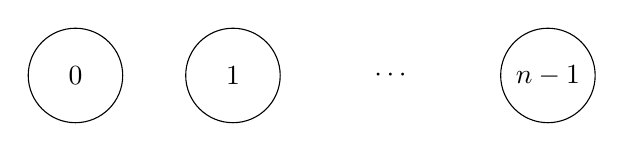
\begin{tikzpicture}
  \node[shape=circle,draw=black,minimum size=1.2cm] (0) at (0,0) {0};
  \node[shape=circle,draw=black,minimum size=1.2cm] (1) at (2,0) {1};
  \node[] (2) at (4,0) {$\cdots$};
  \node[shape=circle,draw=black,minimum size=1.2cm] (3) at (6,0) {$n-1$};
  \end{tikzpicture}
  \end{center}
\exemple Le graphe \emph{chemin} à $n$ sommets $\mathcal{K}_n$ possède une arête entre
  $i$ et $j\in\interefo{0}{n}$ si et seulement si $j=i+1$.
  \begin{center}
  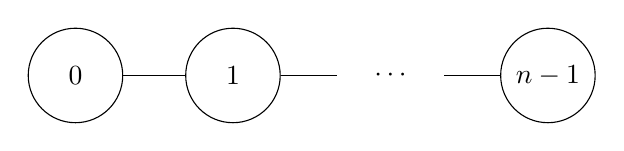
\begin{tikzpicture}
  \node[shape=circle,draw=black,minimum size=1.2cm] (0) at (0,0) {0};
  \node[shape=circle,draw=black,minimum size=1.2cm] (1) at (2,0) {1};
  \node[] (2) at (4,0) {$\quad\cdots\quad$};
  \node[shape=circle,draw=black,minimum size=1.2cm] (3) at (6,0) {$n-1$};
  \path [-](0) edge node[left] {} (1);
  \path [-](1) edge node[left] {} (2);
  \path [-](2) edge node[left] {} (3);
  \end{tikzpicture}
  \end{center}
\exemple Le graphe \emph{cycle} à $n$ sommets $\mathcal{C}_n$ (pour $n\geq 3$) possède une
  arête entre $i$ et $j\in\interefo{0}{n}$ si et seulement si $j\equiv i+1\ [n]$.
  \begin{center}
  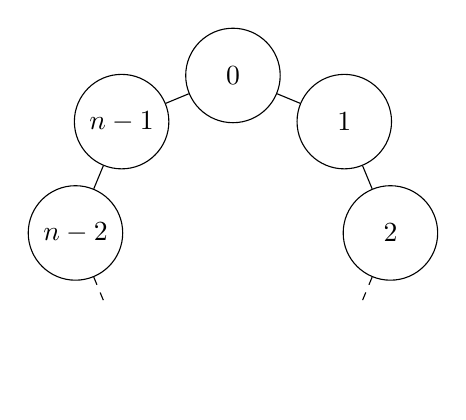
\begin{tikzpicture}
  \node[shape=circle,draw=black,minimum size=1.2cm] (0) at (0,2) {0};
  \node[shape=circle,draw=black,minimum size=1.2cm] (1) at (1.414,1.414) {1};
  \node[shape=circle,draw=black,minimum size=1.2cm] (2) at (2.0,0.0) {2};
  \node[shape=circle,draw=white,minimum size=1.2cm] (3) at (1.414,-1.414) {};
  \node[shape=circle,draw=white,minimum size=1.2cm] (4) at (-1.414,-1.414) {};
  \node[shape=circle,draw=black,minimum size=1.2cm] (5) at (-2,0) {$n-2$};
  \node[shape=circle,draw=black,minimum size=1.2cm] (6) at (-1.414,1.414) {$n-1$};
  \path [-](0) edge node[left] {} (1);
  \path [-](1) edge node[left] {} (2);
  \path [-,dashed](2) edge node[left] {} (3);
  \path [-,dashed](4) edge node[left] {} (5);
  \path [-](5) edge node[left] {} (6);
  \path [-](6) edge node[left] {} (0);
  \end{tikzpicture}
  \end{center}
\exemple Le graphe des utilisateurs de Facebook a un sommet pour chaque utilisateur
  et une arête entre deux sommets lorsque deux utilisateurs sont \emph{amis}. Notons que
  $\abs{S}$ est de l'ordre de $10^9$ et que $\abs{A}$ est de l'ordre
  de $10^{11}$, ce qui pose quelques difficultés algorithmiques.
\exemple Dans le graphe du métro parisien, les sommets représentent les stations de
  métro et les arêtes, les liaisons entre ces stations.
\begin{center}
  \includegraphics[width=0.8\textwidth]{../../Commun/Images/python-cours-metro-paris}
\end{center}
\end{exemples}


\begin{definition}
On appelle \emph{degré} d'un sommet $x$ le nombre d'arêtes de la forme $x-y$.
\end{definition}

\begin{remarqueUnique}
\remarque Le degré d'un sommet est son nombre de voisins.
\end{remarqueUnique}

\begin{definition}
On appelle \emph{chemin} de longueur $n$ toute suite $c\defeq z_0,z_1,\ldots,z_{n}$ de $n+1$ sommets telle que
\[\forall k\in\interefo{0}{n}\qsep z_k-z_{k+1}\in A.\]
Les sommets $z_0$ et $z_n$ sont appelés \emph{extrémités} du chemin et on dit que $c$
\emph{relie} $z_0$ à $z_n$. 
\end{definition}

\begin{remarques}
\remarque On peut aussi voir un chemin de longueur $n$ comme une suite de $n$ arêtes consécutives. Un chemin de longueur $n$ est constitué de $n+1$ sommets et de $n$ arêtes.
\remarque On accepte les chemins de longueur nulle, reliant un sommet à lui-même, sans arête.
\remarque Dans la suite, on notera $l(c)$ la longueur d'un chemin $c$.
\end{remarques}

\begin{definition}
Un chemin $z_0,z_1,\ldots,z_n$ est dit
\begin{itemize}
\item \emph{élémentaire} lorsqu'il ne passe pas deux fois par le même sommet, c'est-à-dire
  lorsque les sommets sont deux à deux distincts.
\item \emph{simple} s'il ne passe pas deux fois par la même arête, c'est-à-dire lorsque
  les arêtes $z_k - z_{k+1}$ sont deux à deux distinctes.
\end{itemize}
\end{definition}

\begin{remarqueUnique}
\remarque Tout chemin élémentaire est simple. Cependant la réciproque est fausse puisque
sur le graphe non orienté ci-dessous, le chemin $0-1-2-3-1-4$ est simple, mais pas
élémentaire.
\begin{center}
  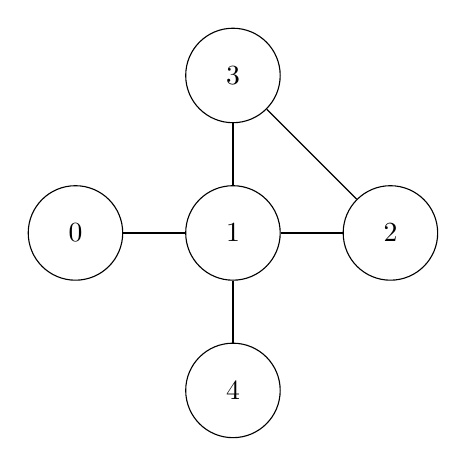
\begin{tikzpicture}
  \node[shape=circle,draw=black,minimum size=1.2cm] (0) at (-2,0) {0};
  \node[shape=circle,draw=black,minimum size=1.2cm] (1) at (0,0) {1};
  \node[shape=circle,draw=black,minimum size=1.2cm] (2) at (0,2) {3};
  \node[shape=circle,draw=black,minimum size=1.2cm] (3) at (2,0) {2};
  \node[shape=circle,draw=black,minimum size=1.2cm] (4) at (0,-2) {4};
  \path [-](0) edge node[left] {} (1);
  \path [-](1) edge node[left] {} (2);
  \path [-](2) edge node[left] {} (3);
  \path [-](3) edge node[left] {} (1);
  \path [-](1) edge node[left] {} (4);
  \end{tikzpicture}
\end{center}
\end{remarqueUnique}

\begin{definition}
Un sommet $y$ est dit \emph{accessible}
depuis un sommet $x$ lorsqu'il existe au moins un chemin
reliant $x$ à $y$.
\end{definition}

\begin{remarqueUnique}
\remarque Puisqu'on accepte les chemins de longueur nulle, tout sommet est
  accessible depuis lui-même.
\end{remarqueUnique}

\begin{proposition}
Dans un graphe non orienté, la relation d'accessibilité est une relation d'équivalence
sur $S$. 
\end{proposition}

\begin{remarques}
\remarque Si $y$ est accessible depuis $x$, alors $x$ est
  accessible depuis $y$. On dit alors que $x$ et $y$ sont \emph{connectés}.
\remarque On appelle \emph{composante connexe} toute classe d'équivalence
pour cette relation.
\end{remarques}

\begin{definition}
On dit qu'un graphe non orienté est \emph{connexe} lorsqu'il ne possède qu'une seule
composante connexe, c'est-à-dire lorsque tous ses sommets sont connectés.
\end{definition}

\begin{definition}
Si $y$ est un sommet accessible depuis un sommet $x$, on appelle distance entre $x$ et
$y$ l'entier
\[{\rm d}(x, y) \defeq \inf \ensim{l(c)}{c
      \textnormal{ est un chemin de } x \textnormal{ à } y}.\]
Un \emph{chemin de longueur minimale} de $x$ à $y$ est un chemin $c$
de $x$ à $y$ tel que $l(c) = {\rm d}(x, y)$.
\end{definition}

\begin{remarques}
\remarque Lorsque $y$ n'est pas accessible depuis $x$, la convention est de poser
  ${\rm d}(x, y)\defeq +\infty$.
\remarque Conformément à ce qu'on attend d'une distance
  \begin{eqnarray*}
  \forall x\in S,& & {\rm d}(x, x)=0,\\
  \forall x,y\in S,& & {\rm d}(y, x)={\rm d}(x, y),\\
  \forall x,y,z\in S,& & {\rm d}(x, z)\leq {\rm d}(x, y)+{\rm d}(y, z).\\
  \end{eqnarray*}
\end{remarques}

\begin{definition}
On appelle \emph{cycle} tout chemin simple de longueur non nulle dont les deux
extrémités sont identiques.
\end{definition}
  
\begin{remarques}
\remarque Dans la définition, il est nécessaire de se limiter aux chemins simples, sinon
  on pourrait construire des \og cycles \fg dans les graphes 
  en parcourant une même arête dans un sens puis dans l'autre.
\remarque Dans un graphe non orienté, la longueur d'un cycle est supérieure ou égale à 3.
\remarque Un cycle sera dit \emph{élémentaire} lorsque la seule répétition de sommets est celle de
  ses extrémités. Un cycle est élémentaire si et seulement si il ne contient pas
  d'autre cycle.
\item On dit qu'un graphe est \emph{acyclique} lorsqu'il ne possède pas de cycle.
\end{remarques}

\begin{exempleUnique}
\exemple Dans le graphe suivant, le chemin $4- 5- 6- 9- 8- 6- 4$ est un cycle. Ce graphe possède 4 cycles élémentaires.
\begin{center}
  \includegraphics[width=6cm]{../../Commun/Images/python-cours-graphe-chemins-et-cycles.pdf}
\end{center}
\end{exempleUnique}

\begin{definition}
On appelle \emph{arbre} tout graphe connexe acyclique.
\end{definition}

\begin{remarques}
\remarque Les graphes suivants sont des arbres.
\begin{center}
\includegraphics[width = 10cm]{../../commun/images/info-cours-graphe-theorie-foret}
\end{center}
\remarque Les arbres que nous avons manipulés dans les chapitres précédents sont ce
  qu'on appelle des \emph{arbres enracinés}. Ce sont des arbres
  pour lesquels on a choisi un sommet appelé \emph{racine}. 
  La distance d'un sommet à la racine est appelée \emph{profondeur}.
  Ces arbres sont conventionnellement dessinés de façon à ce que les sommets de même
  profondeur soient à même hauteur.
\end{remarques}
\vspace{2ex}
\begin{exoUnique}
\exo En choisissant successivement trois racines pour l'arbre de gauche ci-dessus, dessiner
  l'arbre enraciné ainsi obtenu de manière conventionnelle.
\end{exoUnique}

\subsection{Graphe orienté}

\begin{definition}
On appelle \emph{graphe orienté} tout couple $G\defeq\p{S,A}$ où
\begin{itemize}
\item $S$ est un ensemble fini non vide dont les éléments sont appelés
  \emph{sommets}.
\item $A$ est un ensemble de couples $\p{x,y}$, où $x$ et $y$ sont deux éléments
  distincts de $S$. Ces paires sont appelées \emph{arcs}.
\end{itemize}
\end{definition}
    
\begin{remarques}
\remarque En pratique, l'arc $(x,y)$ sera noté $x\to y$ ou $xy$. Intuitivement, un arc
  $x\to y$ permet de passer du sommet $x$ au sommet $y$ mais pas
  du sommet $y$ au sommet $x$. S'il y a un arc $x\to y$, on dit que $x$ est un
  \emph{prédécesseur} de $y$ et que $y$ est un \emph{successeur} de $x$.
\remarque Dans un graphe orienté
  \[\abs{A}\leq \abs{S}\p{\abs{S}-1}.\]
\remarque En pratique, on confondra souvent un graphe
  non orienté $G\defeq(S, A)$ avec son graphe orienté associé $G_{\rm o}$.
  Ce dernier possède les mêmes sommets que $G$. De plus, $x\to y$ est un arc de $G_{\rm o}$ si et
  seulement si $x-y\in A$. En particulier, dans $G_{\rm o}$,  dès que $x\to y$ est un arc,
  $y\to x$ en est un autre.
\remarque Les arbres enracinés s'orientent naturellement depuis leur racine~: lorsqu'on
  les dessine de manière conventionnelle, on les oriente du haut vers le bas. 
\remarque À un graphe orienté $G\defeq(S, A)$, on associe le graphe non orienté
  $G_{\rm no}$ obtenu en \og oubliant \fg l'orientation des arcs.
\end{remarques}
    
\begin{exemples}
\exemple Voici un exemple de graphe orienté à 7 sommets. C'est sur cet exemple que nous
  détaillerons l'exécution de nos algorithmes dans la seconde partie de ce chapitre.
\begin{center}
\begin{tikzpicture}
\node[shape=circle,draw=black,minimum size=1.2cm] (0) at (0,0) {0};
\node[shape=circle,draw=black,minimum size=1.2cm] (1) at (2,0) {1};
\node[shape=circle,draw=black,minimum size=1.2cm] (2) at (4,0) {2};
\node[shape=circle,draw=black,minimum size=1.2cm] (3) at (0,-2) {3};
\node[shape=circle,draw=black,minimum size=1.2cm] (4) at (2,-2) {4};
\node[shape=circle,draw=black,minimum size=1.2cm] (5) at (4,-2) {5};
\node[shape=circle,draw=black,minimum size=1.2cm] (6) at (6,-2) {6};
\path [-{Latex[length=3mm]}](0) edge node[left] {} (1);
\path [-{Latex[length=3mm]}](1) edge node[left] {} (2);
\path [-{Latex[length=3mm]}](0) edge node[left] {} (3);
\path [-{Latex[length=3mm]}](3) edge node[left] {} (4);
\path [-{Latex[length=3mm]}](2) edge node[left] {} (4);
\path [-{Latex[length=3mm]}](4) edge node[left] {} (1);
\path [-{Latex[length=3mm]}](2) edge node[left] {} (5);
\path [-{Latex[length=3mm]}](6) edge node[left] {} (2);
\end{tikzpicture}
\end{center}
\exemple Le graphe du web possède un sommet pour chaque page web et un arc de $x$ vers $y$
  lorsque la page $x$ contient un lien vers la page $y$. C'est ce graphe que les moteurs
  de recherche parcourent pour construire leur index. La taille du graphe du web est inconnue
  mais Google indexe plus de 50 milliards de pages.
\exemple Le graphe des utilisateurs d'Instagram a un sommet pour chaque utilisateur
  et un arc de $x$ vers $y$ lorsque $x$ est un \emph{follower} de $y$. Contrairement
  au graphe des utilisateurs de Facebook qui est non orienté, celui
  d'Instagram l'est.
\end{exemples}

\begin{definition}
Dans un graphe orienté, on appelle
\begin{itemize}
\item \emph{degré entrant} d'un sommet $x$, le nombre d'arcs de la forme $y\to x$.
\item \emph{degré sortant} d'un sommet $x$, le nombre d'arcs de la forme $x\to y$.
\item \emph{degré total} d'un sommet, la somme de son degré entrant et de son degré sortant.
\end{itemize}
\end{definition}

\begin{remarqueUnique}
\remarque Le degré entrant d'un sommet est son nombre de prédécesseurs et le
  degré sortant, son nombre de successeurs.
\end{remarqueUnique}

\begin{definition}
On appelle
chemin de longueur $n$ toute suite $c\defeq z_0,z_1,\ldots,z_{n}$ de $n+1$ sommets telle que
\[\forall k\in\interefo{0}{n}\qsep z_k \to z_{k+1}\in A.\]
Les sommets $z_0$ et $z_n$ sont appelés \emph{extrémités} du chemin et on dit que $c$
\emph{relie} $z_0$ à $z_n$. 
\end{definition}

\begin{remarques}
\remarque Comme dans les graphes non orientés, on définit la notion de chemin
  \emph{élémentaire} et de chemin \emph{simple}. Les chemins élémentaires sont simples,
  mais la réciproque est fausse.
\remarque La notion d'\emph{accessibilité} se définit aussi de la même manière. Cependant,
  dans un graphe orienté, ce n'est plus une relation d'équivalence sur $S$.
  Les notions de connexité et de composante connexe n'ont plus de sens
  pour ces graphes.
\remarque La notion de distance entre un sommet $x$ et un sommet $y$ est toujours définie. L'inégalité triangulaire reste vraie, mais
  la distance n'est plus symétrique.
\remarque La notion de cycle se définit toujours de la même manière dans un graphe
  orienté. Cependant, contrairement à ce qui se passe dans le cas des graphes non orientés,
  il existe des cycles de longueur 2.
\end{remarques}

\subsection{Graphe pondéré}

\begin{definition}
  On appelle \emph{graphe pondéré} la donnée d'un graphe
  $G\defeq\p{S,A}$ et d'une application
  $\rho:A\to\RP$ appelée \emph{poids}.
  \end{definition}



\begin{exempleUnique}
\exemple Voici le graphe non orienté des connexions ferroviaires françaises, le poids
  représentant les temps de trajet en dizaines de minutes.
\begin{center}
\includegraphics[width=0.5\textwidth]{../../Commun/Images/python-cours-france-train}\\
\end{center}
\end{exempleUnique}

\begin{remarques}
\remarque Un graphe pondéré peut être orienté ou non orienté.
\remarque Il est possible de considérer des graphes pondérés avec des fonctions de poids
  prenant des valeurs négatives. Mais dans ce cours, puisque c'est une condition pour
  pouvoir
  appliquer l'algorithme de Dijkstra, nous nous limiterons à des fonctions de poids
  positives.
\remarque On appelle \emph{poids du chemin} $c\defeq z_0,z_1,\ldots,z_n$ le réel
  positif
  \[\rho(c)\defeq \sum_{k=0}^{n-1} \rho(z_k z_{k+1}).\]
\remarque On appelle \emph{poids d'un graphe} la somme des poids de ses arêtes.
\end{remarques}

\begin{definition}
  Si $y$ est un sommet accessible depuis un sommet $x$, on définit
  \[\delta(x, y) \defeq \inf \ensim{\rho(c)}{c
        \textnormal{ est un chemin de } x \textnormal{ à } y}.\]
  Un \emph{chemin de poids minimal} de $x$ à $y$ est un chemin $c$
  de $x$ à $y$ tel que $\rho(c) = \delta(x, y)$.
\end{definition}

\begin{remarqueUnique}
\remarque Dans le cas où les poids sont des distances, par exemple
  si $G$ est le graphe d'un réseau routier, on pourra parler de distance et de plus court
  chemin. Il ne faut cependant pas confondre le réel $\delta(x,y)$ avec l'entier
  ${\rm d}(x,y)$ représentant le nombre minimal d'arcs entre $x$ et $y$.
\end{remarqueUnique}
  
\subsection{Représentation d'un graphe}


\begin{definition}
Soit $G\defeq\p{S,A}$ un graphe où $S=\interefo{0}{n}$. On appelle matrice d'adjacence la matrice $M\in\mat{n}{\Z}$ définie par
\[\forall i,j\in\interefo{0}{n} \qsep m_{i,j}\defeq\begin{cases}
  1 & \text{si $j$ est un successeur de  $i$,}\\
  0 & \text{sinon.}
\end{cases}\]
\end{definition}

\begin{remarques}
\remarque Un graphe est \og non orienté \fg si et seulement si sa matrice d'adjacence est symétrique.
\remarque Puisqu'on interdit les boucles, une matrice d'adjacence n'a
  que des 0 sur la diagonale.
\remarque On peut représenter un graphe pondéré par une matrice d'adjacence $M\in\mat{n}{\R}$. On prend
    pour coefficient $m_{i,j}$ la valeur \verb!None! lorsqu'il n'existe pas d'arc
    de $i$ à $j$, et le poids $\rho_{i,j}$ de l'arc allant de $i$ à $j$
    lorsqu'un tel arc existe. 
\end{remarques}

\begin{definition}
Soit $G\defeq\p{S,A}$ un graphe où $S=\interefo{0}{n}$. On appelle liste d'adjacence le tableau $g$ de longueur
$n$ tel que
pour tout $i\in\interefo{0}{n}$, $g_i$ est la liste des successeurs $j\in\interefo{0}{n}$
de $i$.
\end{definition}

\begin{remarqueUnique}
\remarque On peut représenter un graphe pondéré par une liste d'adjacence
    dans laquelle, pour tout sommet $i$, $g_i$ est la liste des couples
    $(\rho_{i,j},j)$ où $j$ est un successeur de $i$.
\remarque Dans la suite de ce
    cours, nous utiliserons des listes d'adjacence pour stocker les graphes pondérés.
\end{remarqueUnique}


\section{Algorithmes sur les graphes}

\subsection{Parcours générique d'un graphe}

Supposons que vous êtes enfermé dans un labyrinthe de salles, connectées entre elles
par des portes. Nous représentons ce labyrinthe par un graphe dont les sommets sont
les salles et les arêtes sont les portes reliant ces salles entre elles. Si l'on souhaite sortir de ce labyrinthe,
un réflexe naturel est d'emprunter au hasard les portes que l'on croise. Cependant,
cette stratégie possède deux défauts importants~: elle ne nous dit pas ce qu'on doit
faire lorsqu'on tombe dans un cul-de-sac et elle ne nous empêche pas de tourner en rond.\\

Pour résoudre ces deux problèmes, la solution la plus simple est de marquer les
salles. Au cours de notre exploration, nous choisirons donc de les placer
successivement dans 3 états différents~:
\begin{itemize}
\item \emph{Inconnu}~: C'est l'état dans lequel est une salle qui n'a pas encore été
  découverte.
\item \emph{Découvert}~: C'est l'état dans lequel on place une salle lorsqu'on l'a aperçue
  par une porte.
\item \emph{Visité}~: C'est l'état dans lequel est une salle dans laquelle nous sommes
  déjà entrés.
\end{itemize}
Pour ne pas tourner en rond, il suffit de ne pas entrer dans une salle qui a déjà
été visitée. Pour ces salles, on peut choisir de marquer leur sol d'une croix blanche.
Et pour savoir que faire lorsqu'on est dans un cul-de-sac, il suffit de garder une trace
des salles que l'on a découvertes, mais qui n'ont pas encore été visitées. Pour cela, on
conserve avec nous un sac contenant une marque pour chacune d'elles.\\

Revenons au vocabulaire des graphes. À l'aide de ces deux outils, notre sac ainsi que le
marquage des sommets, nous sommes armés pour parcourir l'ensemble des sommets accessibles
depuis notre sommet de départ. Ce sommet est appelé \emph{source}. Pour cela, il
nous suffit de suivre
l'algorithme suivant, que nous appelons \og \emph{parcours générique} \fg.
% \begin{center}
% \begin{minipage}{0.5\linewidth}
% \begin{algorithm}[H]
% \caption{Parcours générique}
% \begin{algorithmic}
% \State mettre le sommet \emph{source} dans le \emph{sac}
% \While{le \emph{sac} n'est pas vide}
%   \State prendre un sommet $x$ dans le $sac$
%   \If{$x$ n'a pas été visité}
%     \State marquer le sommet $x$ comme visité
%     \For{chaque arc $xy$}
%       \State mettre le sommet $y$ dans le sac
%     \EndFor 
%   \EndIf
% \EndWhile
% \end{algorithmic}
% \end{algorithm}
% \end{minipage}
% \end{center}
\begin{center}
  \includegraphics[width=0.5\textwidth]{../../Commun/Images/python-cours-parcours_generique}
\end{center}
\vspace{2ex}
\noindent
La seule propriété dont notre sac a besoin est qu'on puisse y mettre des
sommets pour les extraire plus tard. L'ordre dans lesquels ces sommets sont extraits
n'a pas d'importance pour le moment.

\begin{proposition}
L'algorithme de parcours générique visite tous les sommets accessibles depuis la source
et uniquement ceux-là.
\end{proposition}

Supposons que l'on garde en mémoire le sommet depuis lequel on visite chaque sommet,
en ne mettant pas le sommet $y$ dans notre sac, mais plutôt le couple $(x, y)$.
Un parcours
générique mettra ainsi en valeur un arbre, enraciné en la source, couvrant l'ensemble des
sommets accessibles. Par exemple, en considérant
le graphe ci-dessous,

\begin{center}
\begin{tikzpicture}
\node[shape=circle,draw=black,minimum size=1.2cm] (0) at (0,0) {0};
\node[shape=circle,draw=black,minimum size=1.2cm] (1) at (2,0) {1};
\node[shape=circle,draw=black,minimum size=1.2cm] (2) at (4,0) {2};
\node[shape=circle,draw=black,minimum size=1.2cm] (3) at (0,-2) {3};
\node[shape=circle,draw=black,minimum size=1.2cm] (4) at (2,-2) {4};
\node[shape=circle,draw=black,minimum size=1.2cm] (5) at (4,-2) {5};
\node[shape=circle,draw=black,minimum size=1.2cm] (6) at (6,-2) {6};
\path [-{Latex[length=3mm]}](0) edge node[left] {} (1);
\path [-{Latex[length=3mm]}](1) edge node[left] {} (2);
\path [-{Latex[length=3mm]}](0) edge node[left] {} (3);
\path [-{Latex[length=3mm]}](3) edge node[left] {} (4);
\path [-{Latex[length=3mm]}](2) edge node[left] {} (4);
\path [-{Latex[length=3mm]}](4) edge node[left] {} (1);
\path [-{Latex[length=3mm]}](2) edge node[left] {} (5);
\path [-{Latex[length=3mm]}](6) edge node[left] {} (2);
\end{tikzpicture}
\end{center}

\noindent
si les couples que l'on sort du sac sont successivement $(\emptyset,0)$, $(0, 1)$,
$(1, 2)$, $(0,3)$, $(2,4)$ et $(2,5)$, on obtient l'arbre enraciné suivant~:

\begin{center}
\begin{tikzpicture}
\node[shape=circle,fill=colorLazoBlue1Light,draw=black,minimum size=1.2cm] (0) at (0,0) {0};
\node[shape=circle,fill=colorLazoBlue1Light,draw=black,minimum size=1.2cm] (1) at (2,0) {1};
\node[shape=circle,fill=colorLazoBlue1Light,draw=black,minimum size=1.2cm] (2) at (4,0) {2};
\node[shape=circle,fill=colorLazoBlue1Light,draw=black,minimum size=1.2cm] (3) at (0,-2) {3};
\node[shape=circle,fill=colorLazoBlue1Light,draw=black,minimum size=1.2cm] (4) at (2,-2) {4};
\node[shape=circle,fill=colorLazoBlue1Light,draw=black,minimum size=1.2cm] (5) at (4,-2) {5};
\node[shape=circle,draw=black,minimum size=1.2cm] (6) at (6,-2) {6};
\path [-{Latex[length=3mm,color=colorLazoPink1]},draw=colorLazoPink1](0) edge node[left] {} (1);
\path [-{Latex[length=3mm,color=colorLazoPink1]},draw=colorLazoPink1](1) edge node[left] {} (2);
\path [-{Latex[length=3mm,color=colorLazoPink1]},draw=colorLazoPink1](0) edge node[left] {} (3);
\path [-{Latex[length=3mm,color=black!30]},draw=black!30](3) edge node[left] {} (4);
\path [-{Latex[length=3mm,color=colorLazoPink1]},draw=colorLazoPink1](2) edge node[left] {} (4);
\path [-{Latex[length=3mm,color=black!30]},draw=black!30](4) edge node[left] {} (1);
\path [-{Latex[length=3mm,color=colorLazoPink1]},draw=colorLazoPink1](2) edge node[left] {} (5);
\path [-{Latex[length=3mm,color=black!30]},draw=black!30](6) edge node[left] {} (2);
\end{tikzpicture}
\end{center}
\noindent
Par la suite, nous utiliserons principalement nos sacs pour y placer des sommets.
Cependant, lors de certains raisonnements, il sera parfois utile de faire comme si on y
avait placé un couple.\\

La structure de données que nous allons utiliser pour implémenter notre sac va déterminer
l'ordre dans lequel les sommets en sont extraits.
\begin{itemize}
\item \emph{Pile}~: Si nous utilisons une pile, pour laquelle c'est le dernier sommet qui
  a été placé dans le sac qui en est extrait, nous obtiendrons ce qu'on appelle
  un \emph{parcours en profondeur}. Bien que tous les parcours nous permettent
  d'obtenir l'ensemble des sommets accessibles depuis un sommet, la simplicité de la
  structure de pile fait que c'est souvent ce parcours que nous utiliserons pour cela.
  Nous verrons aussi que le parcours en profondeur nous permet de détecter les cycles
  dans un graphe.
\item \emph{File}~: Si nous utilisons une file, pour laquelle c'est le premier sommet
  qui a été placé dans le sac qui en est extrait, nous obtiendrons ce qu'on appelle
  un \emph{parcours en largeur}. Ce parcours nous sera utile pour trouver le chemin
  de longueur minimale entre la source et les sommets accessibles depuis cette
  dernière.
\item \emph{File de priorité}~: L'utilisation d'une file de priorité nous permettra
  de découvrir une famille d'algorithmes fonctionnant avec les graphes pondérés. Ils
  se distinguent par les différentes priorités qu'ils utilisent.
  \begin{itemize}
  \item \emph{Dijkstra}~: L'algorithme de Dijkstra nous permet de trouver le chemin
    de poids minimal entre la source et les sommets accessibles depuis cette dernière.
    Pour cela, la
    priorité utilisée est le poids du chemin qui nous a permis de découvrir le sommet.
  \item \emph{Prim}~: L'algorithme de Prim nous permet de trouver un arbre de poids minimal
    couvrant l'ensemble des sommets accessibles. Pour cela, la priorité que nous utiliserons est
    le poids de l'arc qui nous a permis de découvrir le sommet.
  \end{itemize}
\end{itemize}

\vspace{2ex}
Commençons par étudier le plus simple de ces parcours~: le parcours en profondeur.

\subsection{Parcours en profondeur}

\subsubsection{Version itérative}

L'implémentation Python du parcours en profondeur se fait naturellement. On suppose
ici que $\mathcal{S}\defeq\interefo{0}{n}$ et que le graphe est représenté par sa liste
d'adjacence. Pour marquer les sommets, nous utilisons le tableau \emph{visité}, de
longueur $n$, dont tous les éléments sont initialisés à \verb!False!. Pour le sac,
nous utilisons la liste \emph{pile} que nous utilisons, comme son nom l'indique, comme
une pile.

\begin{pythoncodeline}
def profondeur(g, s):
    """profondeur(g: list[list[int]], s: int) -> NoneType"""
    n = len(g)
    visite = [False for _ in range(n)]
    pile = [s]
    while len(pile) != 0:
        x = pile.pop()
        if not visite[x]:
            visite[x] = True
            for y in g[x]:
                pile.append(y)
\end{pythoncodeline}
\noindent
Si l'on souhaite effectuer une action pour chaque
sommet, il suffit de définir une fonction \verb!f(x: int) -> NoneType! que l'on appelle
juste avant l'instruction \verb!visite[x] = True!. Par exemple, si l'on souhaite afficher
à l'écran les sommets visités dans l'ordre de notre parcours, il suffit d'insérer \verb!print(x)! ligne 9.

\begin{center}
\begin{tikzpicture}
\node[shape=circle,draw=black,minimum size=1.2cm] (0) at (0,0) {0};
\node[shape=circle,draw=black,minimum size=1.2cm] (1) at (2,0) {1};
\node[shape=circle,draw=black,minimum size=1.2cm] (2) at (4,0) {2};
\node[shape=circle,draw=black,minimum size=1.2cm] (3) at (0,-2) {3};
\node[shape=circle,draw=black,minimum size=1.2cm] (4) at (2,-2) {4};
\node[shape=circle,draw=black,minimum size=1.2cm] (5) at (4,-2) {5};
\node[shape=circle,draw=black,minimum size=1.2cm] (6) at (6,-2) {6};
\path [-{Latex[length=3mm]}](0) edge node[left] {} (1);
\path [-{Latex[length=3mm]}](1) edge node[left] {} (2);
\path [-{Latex[length=3mm]}](0) edge node[left] {} (3);
\path [-{Latex[length=3mm]}](3) edge node[left] {} (4);
\path [-{Latex[length=3mm]}](2) edge node[left] {} (4);
\path [-{Latex[length=3mm]}](4) edge node[left] {} (1);
\path [-{Latex[length=3mm]}](2) edge node[left] {} (5);
\path [-{Latex[length=3mm]}](6) edge node[left] {} (2);
\end{tikzpicture}
\end{center}

Illustrons son fonctionnement en détail sur un exemple. Le tableau ci-dessous détaille
les différentes étapes du parcours en profondeur du présent graphe à partir du sommet 0.
Le contenu de la \emph{pile} est détaillé lors du passage ligne 6, tout comme
l'ensemble des sommets marqués dans \emph{visité}.

\begin{center}
\begin{tabular}{l|l|l}
\emph{pile} & \emph{visité} & action\\
\hline
\verb_[0]_ & $\ens{}$  & Dépiler 0, le marquer et empiler ses successeurs 1 et 3.\\
\verb_[1, 3]_ & $\ens{0}$ & Dépiler 3, le marquer et empiler son successeur 4.\\
\verb_[1, 4]_ & $\ens{0, 3}$ & Dépiler 4, le marquer et empiler son successeur 1.\\
\verb_[1, 1]_ & $\ens{0, 3, 4}$ & Dépiler 1, le marquer et empiler son successeur 2.\\
\verb_[1, 2]_ & $\ens{0, 1, 3, 4}$ & Dépiler 2, le marquer et empiler ses successeurs 4 et 5.\\
\verb_[1, 4, 5]_ & $\ens{0, 1, 2, 3, 4}$ & Dépiler 5 et le marquer. Il n'a pas de successeur.\\
\verb_[1, 4]_ & $\ens{0, 1, 2, 3, 4, 5}$ & Dépiler 4. Il a déjà été marqué.\\
\verb_[1]_ & $\ens{0, 1, 2, 3, 4, 5}$ & Dépiler 1. Il a déjà été marqué.\\
\verb_[]_ & $\ens{0, 1, 2, 3, 4, 5}$ & \emph{pile} est vide donc l'algorithme se termine.
\end{tabular}
\end{center}
Une fois le parcours terminé, tous les sommets atteignables à partir du sommet 0 ont été
marqués, à savoir $0, 1, 2, 3, 4$ et 5. Inversement, le sommet 6, qui n'est pas atteignable
à partir de 0 n'a pas été marqué. C'est là une propriété fondamentale du parcours en
profondeur. Le graphe ci-dessous met en valeur les sommets visités ainsi que les
arcs empruntés lors de ce parcours.

\begin{center}
\begin{tikzpicture}
\node[shape=circle,fill=colorLazoBlue1Light,draw=black,minimum size=1.2cm] (0) at (0,0) {0};
\node[shape=circle,fill=colorLazoBlue1Light,draw=black,minimum size=1.2cm] (1) at (2,0) {1};
\node[shape=circle,fill=colorLazoBlue1Light,draw=black,minimum size=1.2cm] (2) at (4,0) {2};
\node[shape=circle,fill=colorLazoBlue1Light,draw=black,minimum size=1.2cm] (3) at (0,-2) {3};
\node[shape=circle,fill=colorLazoBlue1Light,draw=black,minimum size=1.2cm] (4) at (2,-2) {4};
\node[shape=circle,fill=colorLazoBlue1Light,draw=black,minimum size=1.2cm] (5) at (4,-2) {5};
\node[shape=circle,draw=black,minimum size=1.2cm] (6) at (6,-2) {6};
\path [-{Latex[length=3mm,color=black!30]},draw=black!30](0) edge node[left] {} (1);
\path [-{Latex[length=3mm,color=colorLazoPink1]},draw=colorLazoPink1](1) edge node[left] {} (2);
\path [-{Latex[length=3mm,color=colorLazoPink1]},draw=colorLazoPink1](0) edge node[left] {} (3);
\path [-{Latex[length=3mm,color=colorLazoPink1]},draw=colorLazoPink1](3) edge node[left] {} (4);
\path [-{Latex[length=3mm,color=black!30]},draw=black!30](2) edge node[left] {} (4);
\path [-{Latex[length=3mm,color=colorLazoPink1]},draw=colorLazoPink1](4) edge node[left] {} (1);
\path [-{Latex[length=3mm,color=colorLazoPink1]},draw=colorLazoPink1](2) edge node[left] {} (5);
\path [-{Latex[length=3mm,color=black!30]},draw=black!30](6) edge node[left] {} (2);
\end{tikzpicture}
\end{center}

\subsubsection{Version récursive}

Le parcours en profondeur est un algorithme fondamentalement récursif dont voici une
implémentation Python~:

\begin{pythoncodeline}
def profondeur_rec(g, visite, x):
    """profondeur_rec(g: list[list[int]], visite: list[bool],
                      x: int) -> NoneType"""
    if not visite[x]:
        visite[x] = True
        for y in g[x]:
            profondeur_rec(g, visite, y)
\end{pythoncodeline}
\noindent
Pour lancer un parcours en profondeur depuis un sommet $s$, on utilisera la fonction
suivante~:
\begin{pythoncodeline}
def profondeur(g, s):
    """profondeur(g: list[list[int]], s: int) -> NoneType"""
    n = len(g)
    visite = [False for _ in range(n)]
    profondeur_rec(g, visite, s)
\end{pythoncodeline}
\noindent
Dans cette version, une pile est toujours présente par l'intermédiaire de la pile d'appels.
Contrairement à ce qui se passe dans la version itérative, les sommets sont visités dès
qu'ils sont découverts; en récursif, ces deux états sont donc confondus.
Le tableau ci-dessous détaille l'ensemble des sommets marqués dans \emph{visité} au
moment de l'appel de \verb!profondeur_rec!.
La pile d'appel est aussi représentée dans la colonne \og chemin emprunté \fg.


\begin{center}
\begin{tabular}{l|l|l}
\emph{visité} & chemin emprunté & action\\
\hline
$\ens{}$ &0 &  Marquer 0, emprunter l'arc $0\to 1$.\\
$\ens{0}$ &$0 \to 1$ & Marquer 1, emprunter l'arc $1\to 2$.\\ 
$\ens{0,1}$ &$0 \to 1 \to 2$ & Marquer 2, emprunter l'arc $2\to 4$.\\
$\ens{0, 1, 2}$ &$0 \to 1 \to 2 \to 4$ & Marquer 4, emprunter l'arc $4\to 1$.\\
$\ens{0, 1, 2, 4}$ &$0 \to 1 \to 2 \to 4 \to 1$ & Déjà découvert.\\
$\ens{0,1,2,4}$ &$0 \to 1 \to 2 \to 4$ & Pas d'autre arc, terminé.\\
$\ens{0,1,2,4}$ &$0 \to 1 \to 2$ & Emprunter l'arc $2\to 5$.\\
$\ens{0,1,2,4,5}$ &$0 \to 1 \to 2 \to 5$ & Marquer 5, aucun arc, terminé.\\
$\ens{0,1,2,4,5}$ &$0 \to 1 \to 2$ & Pas d'autre arc, terminé.\\
$\ens{0,1,2,4,5}$ &$0 \to 1$ & Pas d'autre arc, terminé.\\
$\ens{0,1,2,4,5}$ &$0$ & Emprunter l'arc $0\to 3$.\\ 
$\ens{0,1,2,4,5}$ &$0 \to 3$ & Marquer 3, emprunter l'arc $3\to 4$.\\
$\ens{0,1,2,3,4,5}$ & $0 \to 3 \to 4$ & Déjà découvert.\\
$\ens{0,1,2,3,4,5}$ & $0 \to 3$ & Pas d'autre arc, terminé.\\
$\ens{0,1,2,3,4,5}$ & $0$ & Pas d'autre arc, terminé.
\end{tabular}
\end{center}
\noindent
\noindent
On remarque que même si les sommets visités sont les mêmes que dans la version itérative,
les arcs empruntés diffèrent~: le parcours que l'on vient
d'effectuer est un autre parcours en profondeur.


\begin{center}
\begin{tikzpicture}
\node[shape=circle,fill=colorLazoBlue1Light,draw=black,minimum size=1.2cm] (0) at (0,0) {0};
\node[shape=circle,fill=colorLazoBlue1Light,draw=black,minimum size=1.2cm] (1) at (2,0) {1};
\node[shape=circle,fill=colorLazoBlue1Light,draw=black,minimum size=1.2cm] (2) at (4,0) {2};
\node[shape=circle,fill=colorLazoBlue1Light,draw=black,minimum size=1.2cm] (3) at (0,-2) {3};
\node[shape=circle,fill=colorLazoBlue1Light,draw=black,minimum size=1.2cm] (4) at (2,-2) {4};
\node[shape=circle,fill=colorLazoBlue1Light,draw=black,minimum size=1.2cm] (5) at (4,-2) {5};
\node[shape=circle,draw=black,minimum size=1.2cm] (6) at (6,-2) {6};
\path [-{Latex[length=3mm,color=colorLazoPink1]},draw=colorLazoPink1](0) edge node[left] {} (1);
\path [-{Latex[length=3mm,color=colorLazoPink1]},draw=colorLazoPink1](1) edge node[left] {} (2);
\path [-{Latex[length=3mm,color=colorLazoPink1]},draw=colorLazoPink1](0) edge node[left] {} (3);
\path [-{Latex[length=3mm,color=black!30]},draw=black!30](3) edge node[left] {} (4);
\path [-{Latex[length=3mm,color=colorLazoPink1]},draw=colorLazoPink1](2) edge node[left] {} (4);
\path [-{Latex[length=3mm,color=black!30]},draw=black!30](4) edge node[left] {} (1);
\path [-{Latex[length=3mm,color=colorLazoPink1]},draw=colorLazoPink1](2) edge node[left] {} (5);
\path [-{Latex[length=3mm,color=black!30]},draw=black!30](6) edge node[left] {} (2);
\end{tikzpicture}
\end{center}

\subsubsection{Accessibilité, connexité}

Une application immédiate du parcours en profondeur consiste à déterminer s'il existe un
chemin entre deux sommets $x$ et $y$. Pour cela, il suffit de lancer un parcours
en profondeur à partir du sommet $x$ puis, une fois qu'il est terminé, de regarder si le
sommet $y$ fait partie des sommets visités. Le programme suivant
réalise cet algorithme~:

\begin{pythoncodeline}
def existe_chemin(g, x, y):
    """existe_chemin(g: list[list[int]], x: int, y: int) -> bool""" 
    n = len(g)
    visite = [False for _ in range(n)]
    profondeur_rec(g, visite, x)
    return visite[y]
\end{pythoncodeline}

\noindent
Le parcours en profondeur 
est un algorithme très efficace, dont la complexité
temporelle est de l'ordre du nombre de sommets du graphe (pour l'initialisation de \emph{visité})
auquel on ajoute le nombre d'arcs qui sont examinés pendant ce parcours. On a donc une
complexité temporelle 
en ${\rm O}(\abs{S}+\abs{A})$. En effet, chaque arc
$x\to y$ est examiné au plus une fois, à savoir la première fois que la fonction
\verb!profondeur_rec! est appelée sur le sommet $x$~: si la fonction
\verb!profondeur_rec! est rappelée plus tard sur ce même sommet $x$, alors il
sera trouvé dans \emph{visité} et la fonction se terminera immédiatement. Dans le pire des cas, tous les sommets sont atteignables et le graphe
est entièrement parcouru. Le cout est moindre lorsque certains sommets ne sont pas atteignables
depuis le sommet de départ.\\

La complexité spatiale de la version récursive est en $\Theta(\abs{S})$~: cette
complexité provient du tableau \emph{visité} dont
la taille est $\abs{S}$, auquel on ajoute la taille de la pile
d'appels qui reste toujours inférieure au nombre de sommets puisque la succession de
sommets passés en argument des appels actifs forme à
chaque instant un chemin élémentaire.\\

On peut aussi tester la connexité d'un graphe non orienté de la même manière. On utilise pour
cela la fonction \verb!est_connexe!~:
\begin{pythoncodeline}
def tous_vrai(t):
    """tous_vrai(t: list[bool]) -> bool"""
    for v in t:
        if not v:
            return False
    return True

def est_connexe(g):
    """est_connexe(g: list[list[int]]) -> bool"""
    n = len(g)
    visite = [False for _ in range(n)]
    profondeur_rec(g, visite, 0)
    return tous_vrai(visite)
\end{pythoncodeline}
\noindent
Cet algorithme a de nouveau une complexité temporelle en ${\rm O}(\abs{S}+\abs{A})$ et
une complexité spatiale en $\Theta(\abs{S})$.

\begin{exoUnique}
\exo Écrire une fonction qui compte le nombre de composantes connexes d'un graphe non
  orienté.
\end{exoUnique}

\subsubsection{Détection de cycle}

Le parcours en profondeur permet également de détecter la présence d'un cycle dans un
graphe orienté. En effet, puisque l'on marque les sommets avant de considérer leurs voisins,
pour justement éviter de tourner en rond dans un cycle, alors on doit pouvoir être à même
de détecter leur présence. Il y a cependant une subtilité, car lorsqu'on retombe
sur un sommet déjà marqué, on ne sait pas pour autant si l'on vient de découvrir un cycle.
Considérons par exemple le parcours en profondeur des deux graphes suivants, à partir
du sommet 0 à chaque fois.

\begin{center}
\begin{tikzpicture}
\node[shape=circle,draw=black,minimum size=1.2cm] (0) at (0,0) {0};
\node[shape=circle,draw=black,minimum size=1.2cm] (1) at (2,2) {1};
\node[shape=circle,draw=black,minimum size=1.2cm] (2) at (4,0) {2};
\node[shape=circle,draw=black,minimum size=1.2cm] (3) at (2,-2) {3};
\path [-{Latex[length=3mm]}](0) edge node[left] {} (1);
\path [-{Latex[length=3mm]}](1) edge node[left] {} (2);
\path [-{Latex[length=3mm]}](0) edge node[left] {} (3);
\path [-{Latex[length=3mm]}](3) edge node[left] {} (2);
\end{tikzpicture}
\hspace{2cm}
\begin{tikzpicture}
\node[shape=circle,draw=black,minimum size=1.2cm] (0) at (0,0) {0};
\node[shape=circle,draw=black,minimum size=1.2cm] (1) at (2,2) {1};
\node[shape=circle,draw=black,minimum size=1.2cm] (2) at (4,0) {2};
\node[shape=circle,draw=black,minimum size=1.2cm] (3) at (2,-2) {3};
\path [-{Latex[length=3mm]}](0) edge node[left] {} (1);
\path [-{Latex[length=3mm]}](1) edge node[left] {} (2);
\path [-{Latex[length=3mm]}](3) edge node[left] {} (1);
\path [-{Latex[length=3mm]}](2) edge node[left] {} (3);
\end{tikzpicture}
\end{center}
\noindent
Dans le graphe de gauche, on retombe sur le sommet 2. Il n'y a pas de cycle pour autant,
mais seulement un chemin parallèle. Dans le graphe de droite, on retombe sur
le sommet 1, cette fois à cause d'un cycle. Tel qu'il est écrit, notre parcours en
profondeur ne nous permet de pas distinguer ces deux situations. Dans les deux cas, 
on constate que le sommet est déjà visité sans pouvoir en tirer de conclusion quant à
l'existence d'un cycle.\\

Pour y remédier, on va distinguer dans notre marquage trois sortes de sommets~:
ceux que l'on n'a pas encore découverts qui seront marqués comme \emph{inconnu}, ceux que
l'on a \emph{découvert} mais qui sont toujours présents dans le chemin déterminé
par la pile d'appels (ces sommets sont donc \emph{visités} puisque nous
utilisons une implémentation récursive dans laquelle ces deux états sont confondus),
et ceux qui ne sont plus présents dans la pile d'appels,
qu'on marquera comme \emph{fermé}.
Le parcours en profondeur est modifié de la manière suivante~: lorsqu'on visite un sommet
$x$
\begin{itemize}
\item S'il est marqué comme \og découvert \fg, c'est qu'on vient de découvrir un cycle.
\item S'il est marqué comme \og fermé \fg, on ne fait rien.
\item S'il est marqué comme \og inconnu \fg, on procède ainsi~:
  \begin{itemize}
  \item On marque le sommet $x$ comme \og découvert \fg.
  \item On visite tous ses successeurs, récursivement.
  \item Enfin, on le marque comme \og fermé \fg.
  \end{itemize}
\end{itemize}
Comme on le voit, les successeurs du sommet $x$ sont examinés après le moment où $x$
est marqué comme \og découvert \fg et avant le moment où il est marqué comme
\og fermé \fg. Ainsi, s'il existe un cycle nous ramenant sur $x$, on le trouvera
comme étant \og découvert \fg et le cycle sera signalé.\\

Le programme suivant réalise cette détection de cycle.
La fonction \verb!possede_cycle_rec(g, x, etat)! est toujours une fonction récursive, mais
elle renvoie désormais un résultat, à savoir un booléen indiquant la présence d'un cycle.
Enfin, la fonction \verb!possede_cycle! marque tous les sommets comme \og inconnu \fg puis
lance un parcours
en profondeur à partir de tous les sommets du graphe. Si l'un de ces parcours renvoie
\verb!True!, on transmet ce résultat. Sinon, on renvoie \verb!False!.
 
\begin{pythoncodeline}
INCONNU = 0
DECOUVERT = 1
FERME = 2

def possede_cycle_rec(g, etat, x):
    """possede_cycle_rec(g: list[list[int]], etat: list[int], x: int) -> bool"""
    if etat[x] == INCONNU:
        etat[x] = DECOUVERT
        for y in g[x]:
            cycle = possede_cycle_rec(g, etat, y)
            if cycle:
                return True
        etat[x] = FERME
        return False
    else:
        return etat[x] == DECOUVERT
\end{pythoncodeline}
\noindent
Enfin, dans la version suivante, on cherche à détecter la présence d'un cycle n'importe
où dans le graphe. C'est pourquoi on lance un parcours en profondeur à partir de tous
les sommets du graphe. 
\begin{pythoncodeline}
def possede_cycle(g):
    """possede_cycle(g: list[list[int]]) -> bool"""
    n = len(g)
    etat = [INCONNU for _ in range(n)]
    for x in range(n):
        cycle = possede_cycle_rec(g, etat, x)
        if cycle:
            return True
    return False
\end{pythoncodeline}
\noindent
Pour beaucoup de ces sommets, le parcours est déjà passé par là, car ils
étaient accessibles depuis des sommets déjà parcourus; la fonction
\verb!parcours_cycle_rec! se termine alors immédiatement sans rien faire. À nouveau,
la complexité temporelle de cet algorithme est en ${\rm O}(\abs{S}+\abs{A})$, et sa complexité spatiale en $\Theta(\abs{S})$.\\

Attention à ne pas oublier que cet algorithme ne fonctionne que pour les graphes orientés.
Il nécessite quelques aménagements pour fonctionner avec les graphes non orientés.

\subsection{Parcours en largeur}

Le parcours en largeur se fait simplement en utilisant une liste pour implémenter le
sac de notre parcours générique~:

\begin{pythoncodeline}
import collections

def largeur(g, s):
    """largeur(g: list[list[int]], s: int) -> NoneType""" 
    n = len(g)
    visite = [False for _ in range(n)]
    file = collections.deque()
    file.append(s)
    while len(file) != 0:
        x = file.popleft()
        if not visite[x]:
            visite[x] = True
            for y in g[x]:
                file.append(y)
\end{pythoncodeline}
\noindent
Illustrons son fonctionnement sur un notre exemple. Le tableau ci-dessous détaille
les différentes étapes du parcours en largeur du graphe précédent à partir du sommet 0.
Le contenu de la \emph{file} est détaillé lors du passage ligne 9, tout comme
l'ensemble des sommets marqués dans \emph{visité}.

\begin{center}
\begin{tabular}{l|l|l}
\emph{file} & \emph{visité} & action\\
\hline
\verb_[0]_ & $\ens{}$  & Défiler 0, le marquer et enfiler ses successeurs 1 et 3.\\
\verb_[1, 3]_ & $\ens{0}$ & Défiler 1, le marquer et enfiler son successeur 2.\\
\verb_[3, 2]_ & $\ens{0, 1}$ & Défiler 3, le marquer et enfiler son successeur 4.\\
\verb_[2, 4]_ & $\ens{0, 1, 3}$ & Défiler 2, le marquer et enfiler ses successeurs 4 et 5.\\
\verb_[4, 4, 5]_ & $\ens{0, 1, 2, 3}$ & Défiler 4, le marquer et empiler son successeurs 1.\\
\verb_[4, 5, 1]_ & $\ens{0, 1, 2, 3, 4}$ & Défiler 4. Il a déjà été marqué.\\
\verb_[5, 1]_ & $\ens{0, 1, 2, 3, 4}$ & Défiler 5, le marquer. Il n'a pas de successeur.\\
\verb_[1]_ & $\ens{0, 1, 2, 3, 4, 5}$ & Défiler 1. Il a déjà été marqué donc on ne fait rien.\\
\verb_[]_ & $\ens{0, 1, 2, 3, 4, 5}$ & \emph{file} est vide donc l'algorithme se termine.
\end{tabular}
\end{center}

\noindent
Tout comme le parcours en profondeur, le parcours en largeur a visité exactement les
sommets atteignables à partir du sommet 0. Voici les sommets visités ainsi que les
arcs empruntés  lors de ce parcours.

\begin{center}
\begin{tikzpicture}
\node[shape=circle,fill=colorLazoBlue2!15,draw=black,minimum size=1.2cm] (0) at (0,0) {0};
\node[shape=circle,fill=colorLazoBlue2!35,draw=black,minimum size=1.2cm] (1) at (2,0) {1};
\node[shape=circle,fill=colorLazoBlue2!75,draw=black,minimum size=1.2cm] (2) at (4,0) {2};
\node[shape=circle,fill=colorLazoBlue2!35,draw=black,minimum size=1.2cm] (3) at (0,-2) {3};
\node[shape=circle,fill=colorLazoBlue2!75,draw=black,minimum size=1.2cm] (4) at (2,-2) {4};
\node[shape=circle,fill=colorLazoBlue2!110,draw=black,minimum size=1.2cm] (5) at (4,-2) {5};
\node[shape=circle,draw=black,minimum size=1.2cm] (6) at (6,-2) {6};
\path [-{Latex[length=3mm,color=colorLazoPink1]},draw=colorLazoPink1](0) edge node[left] {} (1);
\path [-{Latex[length=3mm,color=colorLazoPink1]},draw=colorLazoPink1](1) edge node[left] {} (2);
\path [-{Latex[length=3mm,color=colorLazoPink1]},draw=colorLazoPink1](0) edge node[left] {} (3);
\path [-{Latex[length=3mm,color=colorLazoPink1]},draw=colorLazoPink1](3) edge node[left] {} (4);
\path [-{Latex[length=3mm,color=black!30]},draw=black!30](2) edge node[left] {} (4);
\path [-{Latex[length=3mm,color=black!30]},draw=black!30](4) edge node[left] {} (1);
\path [-{Latex[length=3mm,color=colorLazoPink1]},draw=colorLazoPink1](2) edge node[left] {} (5);
\path [-{Latex[length=3mm,color=black!30]},draw=black!30](6) edge node[left] {} (2);
\end{tikzpicture}
\end{center}
\noindent
On observe que les arcs ainsi mis en valeur soulignent les chemins de longueur minimale entre
la source 0 et les sommets atteignables depuis cette source. On voit que les sommets
1 et 3 sont à une distance de 1 de la source, les sommets 2 et 4 sont à une distance de 2
et le sommet 5 est à une distance de 3.\\

Comme pour le parcours en profondeur, un même sommet peut apparaitre plusieurs fois
dans notre sac, mais le fait qu'on travaille ici avec une \emph{file} fait que
les sommets sortent de la file dans le même ordre que celui dans lequel ils y sont
entrés. Une fois qu'un sommet y est entré, il est donc inutile de l'enfiler
de nouveau. Cette remarque nous permet l'optimisation suivante~: au lieu de marquer les
sommets lorsqu'ils sont \emph{visités}, c'est-à-dire lorsqu'ils sortent de la file, nous
allons les marquer lorsqu'ils sont \emph{découverts}, c'est-à-dire lorsqu'ils y entrent.

\begin{pythoncodeline}
def largeur(g, s):
    """largeur(g: list[list[int]], s: int) -> NoneType"""
    n = len(g)
    decouvert = [False for _ in range(n)]
    file = collections.deque()
    decouvert[s] = True
    file.append(s)
    while len(file) != 0:
        x = file.popleft()
        for y in g[x]:
            if not decouvert[y]:
                decouvert[y] = True
                file.append(y)
\end{pythoncodeline}
\noindent
Contrairement à l'algorithme initial qu'on appelle parfois parcours en largeur à
marquage \emph{tardif}, cette nouvelle version est appelée parcours en largeur
à marquage \emph{précoce}. Avec cette optimisation, les valeurs successives de
\emph{file} sont~: \verb![0]!, \verb![1, 3]!, \verb![3,2]!, \verb![2, 4]!,
\verb![4, 5]!, \verb![5]! et enfin \verb![]!. On remarque qu'à chaque étape,
la file est composée d'une succession de sommets dont la distance à la source
est $d$ suivie d'une succession (éventuellement vide) de sommets dont la distance à
la source est $d+1$. On observe donc que le parcours en largeur explore le
graphe en \og cercles concentriques\fg à partir de la source.\\

Cette idée de cercles concentriques nous permet une dernière transformation de notre
programme dans lequel on va travailler non pas avec un sac fonctionnant comme une file,
mais avec deux sacs. À chaque instant, un des
sacs, qu'on appelle \emph{courant}, contient des sommets situés à une distance $d$ de
la source, tandis que l'autre sac, qu'on appelle \emph{suivant}, contient des sommets à une
distance $d+1$ de la source. On examinera ces derniers une fois que le sac
\emph{courant} est vide. Par soucis de simplicité, nous utiliserons une pile pour
implémenter ces deux sacs, mais nous aurions pu utiliser n'importe quelle
structure de donnée séquentielle. À côté de ces deux piles, on utilise un tableau \emph{découvert}
qui marque les sommets déjà découverts. Le parcours en largeur procède ainsi~:
\begin{itemize}
\item Initialement, la source est empilée dans \emph{courant} et on la marque comme \emph{découverte}.
\item Tant que la pile \emph{courant} n'est pas vide
\begin{itemize}
  \item On dépile le sommet $x$ de \emph{courant}.
  \item Pour chaque successeur $y$ de $x$, s'il n'a pas été marqué comme \emph{découvert}, on
    le marque et on l'empile dans \emph{suivant}. 
\end{itemize}
\item Si la pile \emph{courant} est vide, on l'échange avec
  la pile \emph{suivant}.
\end{itemize}
Si l'on reprend l'exemple de notre graphe exemple
et qu'on effectue un parcours en largeur à partir du sommet 0, on obtient le parcours
résumé dans le tableau suivant.

\begin{center}
\begin{tabular}{l|l|l|l}
\emph{vu} & \emph{courant} & \emph{suivant} & action\\
\hline
$\emptyset$ &\verb![]! & \verb![]! & Le sommet 0 est marqué puis empilé dans \emph{courant}.\\
$\ens{0}$ &\verb![0]! & \verb![]! &  On dépile le sommet 0; 1 et 3 sont marqués puis empilés dans \emph{suivant}.\\
$\ens{0, 1, 3}$ &\verb![]!   & \verb![1, 3]! & La pile \emph{courant} est vide; on échange.\\
$\ens{0, 1, 3}$ &\verb![1, 3]! &  \verb![]! & On dépile le sommet 3; 4 est marqué puis empilé dans \emph{suivant}.\\
$\ens{0, 1, 3, 4}$&\verb![1]! & \verb![4]! & On dépile le sommet 1; 2 est marqué puis empilé dans \emph{suivant}.\\
$\ens{0, 1, 2, 3, 4}$&\verb![]!   & \verb![4, 2]! & La pile \emph{courant} est vide; on échange.\\
$\ens{0, 1, 2, 3, 4}$&\verb![4, 2]! & \verb![]!  & On dépile le sommet 2; 5 est marqué puis empilé dans \emph{suivant}.\\
$\ens{0, 1, 2, 3, 4, 5}$&\verb![4]! & \verb![5]!  & On dépile le sommet 4.\\
$\ens{0, 1, 2, 3, 4, 5}$&\verb![]! &  \verb![5]! & La pile \emph{courant} est vide; on échange.\\
$\ens{0, 1, 2, 3, 4, 5}$&\verb![5]! &  \verb![]! & On dépile le sommet 5.\\
$\ens{0, 1, 2, 3, 4, 5}$&\verb![]!  &  \verb![]! &  \emph{courant} est vide donc
l'algorithme se termine.
\end{tabular}
\end{center}

\noindent
L'implémentation Python de cet algorithme se fait alors naturellement.

\begin{pythoncodeline}
def largeur(g, s):
    """largeur(g: list[list[int]], s: int) -> NoneType"""
    n = len(g)
    decouvert = [False for _ in range(n)]
    decouvert[s] = True
    courant = [s]
    suivant = []
    while len(courant) != 0:
        x = courant.pop()
        for y in g[x]:
            if not decouvert[y]:
                decouvert[y] = True
                suivant.append(y)
        if len(courant) == 0:
            courant = suivant
            suivant = []
\end{pythoncodeline}
\noindent
Si l'on souhaite effectuer une action pour chaque sommet à l'aide d'une fonction
\verb!f(x: int) -> NoneType!, on l'appellera juste avant d'avoir marqué le sommet
avec l'instruction \verb!decouvert[x] = True!, c'est-à-dire aux lignes 5 et 12.\\

Comme pour le parcours en profondeur, le parcours en largeur a une complexité temporelle
en ${\rm O}(\abs{S}+\abs{A})$ et une complexité spatiale en $\Theta(\abs{S})$. 
En effet, chaque
sommet est placé au plus une fois dans la pile \emph{suivant}, la première fois qu'il est
rencontré.  Donc chaque arc
$x\to y$ est examiné au plus une fois, lorsque le sommet $x$ est retiré de l'ensemble
courant.
\vspace{2ex}
\begin{exoUnique}
\exo Écrire une fonction prenant entrée un graphe et une source et renvoyant le
  tableau des distances de chaque sommet à la source. Le tableau contiendra \verb!None!
  pour un sommet qui n'est pas accessible.
  \begin{sol}
\begin{pythoncodeline}
def distance(g, s):
    """distance(g: list[list[int]], s: int) -> list[int]"""
    n = len(g)
    dist = [None for _ in range(n)]
    dist[s] = 0
    courant = [s]
    suivant = []
    d_suivant = 1
    while len(courant) != 0:
        x = courant.pop()
        for y in g[x]:
            if dist[y] == None:
                dist[y] = d_suivant
                suivant.append(y)
        if len(courant) == 0:
            courant = suivant
            suivant = []
            d_suivant = d_suivant + 1
    return dist
\end{pythoncodeline}
  \end{sol}
\end{exoUnique}

\subsection{Plus court chemin}

Dans cette section, on se donne un graphe pondéré $G\defeq(S,A,\rho)$ ainsi qu'une source
$s$. On rappelle que le fonction de poids avec laquelle on travaille est positive.
On cherche à déterminer pour chaque sommet $x$, le poids minimal d'un chemin reliant $s$
à $x$. Afin d'utiliser une terminologie plus conventionnelle, on imaginera que les poids représentent des
distances et on utilisera les termes de distance et de plus court chemin.

\subsubsection{Algorithme de Dijkstra}

L'implémentation de l'algorithme de Dijkstra se fait simplement en utilisant
une file de priorité pour notre sac dans notre parcours générique. Les priorités
sont des distances et c'est ainsi que nous les appelerons dans notre description.
\begin{itemize}
\item On commence par insérer la source dans la file avec une distance de $0$.
\item Tant que la file de priorité n'est pas vide~:
\begin{itemize}
\item On récupère l'élément $x$ ayant la plus faible distance $\delta$.
\item Si $x$ n'a pas encore été visité~:
  \begin{itemize}
  \item On le marque comme visité. La distance $\delta$ est alors la distance entre la source
    et $x$.
  \item Pour tous ses successeurs $y$, on les insère dans la file de priorité avec
    la distance $\delta+\rho(x\to y)$.
  \end{itemize}
\end{itemize}
\end{itemize}

\vspace{2ex}
Remarquons qu'un même sommet pourra se retrouver plusieurs fois dans la file de
priorité, avec des distances différentes. L'algorithme de parcours ne traitant que les
sommets de la file qui n'en sont pas encore sortis, si l'on insère un sommet $x$ 
avec une distance $\delta'$ et qu'il est déjà présent dans la file avec une distance $\delta\leq \delta'$, cette
insertion n'affecte pas le déroulement de notre programme. Si par contre $\delta'<\delta$, c'est
l'ancien élément présent dans la file qui est ignoré. Tout se passe
donc comme si la distance $\delta$ du sommet $x$ était mise à jour à $\min(\delta,\delta')$.\\

Afin de se familiariser avec cet algorithme, nous allons l'exécuter
sur le graphe suivant, en utilisant le sommet 0 pour source.

\begin{center}
\includegraphics[width=0.3\textwidth]{../../Commun/Images/python-cours-graphe-dikstra.png}
\end{center}

\begin{itemize}
\item On commence à placer le sommet 0 dans la file avec la distance 0.
\item Le seul sommet de la file est le sommet 0. C'est donc celui dont
  la distance est minimale. On marque ce sommet comme visité puis on
  regarde ses voisins~: 1, 2, 3 et 4. On les place dans la file de priorité
  avec les distances respectives de 15, 16, 13 et 9.
\item Le sommet de la file ayant une distance minimale est 4. Cette distance est de 9.
  On le marque comme visité, puis on regarde ses voisins~: 1, 3 et 2.
  Le chemin passant par 4 et allant à 1 a une distance de 16 qui n'est pas inférieure
  à la distance actuelle pour 1. Par contre, le chemin passant par 4 et allant à 3
  a une distance de 12 qui est inférieure à la distance actuelle de 13 pour 3. C'est aussi le
  cas du chemin passant par 4 et allant à 2 dont la distance est 14. On met donc
  ces distances à jour dans notre file. Les sommets de la file sont donc désormais
  les sommets 1, 2, et 3 de distances respectives 15, 14 et 12.
\item Le sommet de la file ayant une distance minimale est 3. Cette distance est de 12.
  Aucun des chemins passant par 3 et menant à ses voisins ne permet d'obtenir une
  meilleure distance que celle que nous avons actuellement.
\item Le sommet de la file ayant une distance minimale est 2. 
  On marque ce sommet comme visité, puis on regarde ses voisins~: 4, 3, 0 et 5. La
  distance du sommet 2 étant 14, on insère donc le sommet 5 avec une distance de 20.
  Les sommets de la file sont désormais les sommets 1 et 5 de distances respectives 15 et 20.
\item Le sommet de la file ayant une distance minimale est 1. Cette distance est de 15.
  On marque ce sommet comme visité, puis on regarde ses voisins~: 0, 4 et 5.
  Le chemin passant par 1 et allant à 5 a une distance de 16 qui est inférieure
  à la distance temporaire de 20. On met donc à jour cette distance.
\item Le sommet de la file ayant une distance minimale est 5. Cette distance est de 16.
  On marque ce sommet comme visité. L'étude de ses voisins ne donne lieu à aucune mise à
  jour, car ils ont déjà tous été traités.
\item À la boucle suivante, il n'y a plus de sommet dans notre file et l'algorithme
  s'arrête. Les distances du sommet 0 aux autres sommets du graphe sont donc 0 pour 0,
  9 pour 4, 12 pour 3, 14 pour 2, 15 pour 1 et 16 pour 5.
\end{itemize}
\vspace{2ex}

Pour l'implémentation, nous utilisons le module \verb!heapq! de Python.

\begin{pythoncodeline}
import heapq

def dijkstra(g, s):
    """dijkstra(g: list[list[tuple[float, int]]], s: int) -> list[float]"""
    n = len(g)
    visite = [False for _ in range(n)]
    dist = [None for _ in range(n)]
    filep = []
    heapq.heappush(filep, (0.0, s))
    while len(filep) != 0:
        delta, x = heapq.heappop(filep)
        if not visite[x]:
            dist[x] = d
            visite[x] = True
            for rho, y in g[x]:
                heapq.heappush(filep, (delta + rho, y))
    return dist
\end{pythoncodeline}

\vspace{2ex}
Si nous ne disposons pas de file de priorité, nous pouvons en faire une implémentation
à la main (qui ne sera malheureusement pas très efficace). Pour cela, nous allons utiliser
deux tableaux \emph{visité} et \emph{dist} dont la longueur est le nombre $n$ de sommets du graphe. Lorsqu'un sommet $x$ est dans l'état \emph{inconnu} c'est-à-dire lorsqu'il
n'a pas encore été inséré dans la liste, \verb!dist[x]! est égal à \verb!None! et
\verb!visite[x]! est égal à \verb!False!. Lorsqu'un sommet $x$ est dans la file,
\verb!dist[x]! contient sa priorité, et \verb!visite[x]! est égal à \verb!False!.
Enfin, lorsque $x$ est sorti de la file de priorité, \verb!dist[x]! contient la distance
de la source au sommet $x$ et \verb!visite[x]! est égal à \verb!True!.
On commence par écrire une fonction \verb!prochain_sommet! qui renvoie le sommet de
la file dont la distance est minimale.

\begin{pythoncodeline}
def prochain_sommet(dist, visite):
    """prochain_sommet(dist: list[float], visite: list[bool]) -> int"""
    n = len(dist)
    min_value = None
    min_x = None
    for x in range(n):
        if (not visite[x]) and (dist[x] != None) \
                and (min_value == None or dist[x] < min_value):
            min_value = dist[x]
            min_x = x
    return min_x
\end{pythoncodeline}
\noindent
L'algorithme de Dijkstra s'écrit alors naturellement.

\begin{pythoncodeline}
def dijkstra(g, s):
    """dijkstra(g: list[list[tuple[float, int]]], s: int) -> list[float]"""
    n = len(g)
    visite = [False for _ in range(n)]
    dist = [None for _ in range(n)]
    dist[s] = 0.0
    while True:
        x = prochain_sommet(dist, visite)
        if x == None:
            break
        visite[x] = True
        for rho, y in g[x]:
            delta = dist[x] + rho
            if dist[y] == None or delta < dist[y]:
                dist[y] = delta
    return dist
\end{pythoncodeline}

\subsubsection{Algorithme ${\rm A}^\star$}

L'algorithme de Dijkstra permet de déterminer la distance d'une source $s$ à
l'ensemble des sommets accessibles depuis $s$. Si l'on s'intéresse uniquement à la
distance entre la source et un but $b$, il est possible d'arrêter l'algorithme dès que
le sommet $b$ est
marqué comme visité. Sur la figure ci-dessous, on a réalisé une recherche du meilleur
chemin dans la ville d'Oldenburg, en Allemagne, en partant d'une source située en centre-ville et pour aller vers un but situé en périphérie, à l'ouest de la ville. Le chemin optimal trouvé est en rouge.

\begin{center}
\includegraphics[width=0.4\textwidth]{../../Commun/Images/python-cours-graphe-astar-1.png}
\end{center}

Nous avons colorié en vert l'ensemble des sommets \og visités \fg par l'algorithme de
Dijkstra. La zone couverte par l'algorithme est formée de tous les points dont
la distance à la source est inférieure à la distance entre $s$ et $b$. Cependant, notre
intuition nous dit qu'il n'est surement pas utile d'aller traiter des sommets qui se
trouvent tout à l'est de la ville alors que notre but est à l'ouest. Cette intuition
se fonde sur le fait que la distance entre deux sommets $x$ et $y$ du graphe est
supérieure à la distance à vol d'oiseau entre ces deux sommets.\\

Pour exploiter cette idée, nous allons définir la fonction $h:S\to\R$, appelée
\emph{heuristique}, par
\[\forall x\in S\qsep h(x)\defeq\norme{x-b}\]
et définir une nouvelle distance $\rho'$ sur $A$ en définissant, pour tout
arc $x\to y$
\[\rho'(x\to y)=\rho(x\to y)+h(y)-h(x).\]
Remarquons tout d'abord que $\rho'$ est bien à valeurs positives puisque si $x\to y$ est
un arc
\[\rho(x\to y)\geq \norme{x-y}\geq \abs{\norme{x-b} - \norme{y-b}}\geq \norme{x-b} - \norme{y-b}=h(x)-h(y),\]
donc $\rho'(x\to y)=\rho(x\to y)+h(y)-h(x)\geq 0$. Remarquons enfin que, quel que
soit le chemin $z_0\to z_1\to\cdots\to z_n$, on a
$\rho'(z_0\to z_1\to\cdots\to z_n)=\rho(z_0\to z_1\to\cdots\to z_n)+h(z_n)-h(z_0)$.
En particulier
\[\rho'(s\to z_1\to\cdots\to z_{n-1}\to b)=\rho(s\to z_1\to\cdots\to z_{n-1}\to b)+h(b)-h(s).\]
Puisque $h(b)-h(s)$ est indépendant du chemin allant de $s$ à $b$,
tout chemin entre ces deux sommets de distance minimale pour $\rho'$ est minimal
pour $\rho$. L'algorithme de Dijkstra appliqué sur le même graphe
avec la distance $\rho'$ au lieu de la distance $\rho$ donnera donc un même chemin
minimal entre $s$ et $b$. Remarquons que cette nouvelle distance va privilégier les
sommets se situant en direction du but. En effet, dans le cas extrême où il existe
une ligne droite entre la source et le but et plusieurs sommets du graphe sont alignés,
la distance entre ces sommets pour la nouvelle distance $\rho'$ va être nulle et ce
sont bien ces sommets qui vont être traités en premier.\\

En reprenant la recherche du meilleur chemin entre le centre et un point de la périphérie
d'Oldenburg, on voit que l'algorithme de Dijkstra appliqué à
nouvelle distance traite beaucoup moins de sommets avant d'arriver sur le but, tout en garantissant le fait que
le chemin trouvé a une distance minimale pour la distance d'origine.

\begin{center}
\includegraphics[width=0.4\textwidth]{../../Commun/Images/python-cours-graphe-astar-2.png}
\end{center}

%END_BOOK
\end{document}




\chapter{Langage Python}
Cette annexe liste limitativement les éléments du langage Python (version 3 ou supérieure) dont la connaissance est exigible des étudiants. Aucun concept sous-jacent n'est exigible au titre de la présente annexe.\\

Aucune connaissance sur un module particulier n'est exigible des étudiants.\\

Toute utilisation d'autres éléments du langage que ceux que liste cette annexe, ou d'une fonction d'un module, doit obligatoirement être accompagnée de la documentation utile, sans que puisse être attendue une quelconque maîtrise par les étudiants de ces éléments.

\subsubsection*{Traits généraux}
\begin{itemize}
\item Typage dynamique~: l'interpréteur détermine le type à la volée lors de l'exécution du code.
\item Principe d'indentation.
\item Portée lexicale~: lorsqu'une expression fait référence à une variable à l'intérieur d'une fonction, Python cherche la valeur définie à l'intérieur de la fonction et à défaut la valeur dans l'espace global du module.
\item Appel de fonction par valeur~: l'exécution de \verb|f(x)| évalue d'abord $x$ puis exécute $f$ avec la valeur calculée.
\end{itemize}

\subsubsection*{Types de base}
\begin{itemize}
\item Opérations sur les entiers (\verb|int|)~: \verb|+|, \verb|-|, \verb|*|, \verb|//|, \verb|**|, \verb|%| avec des opérandes positifs.
\item Opérations sur les flottants (\verb|float|)~: \verb|+|, \verb|-|, \verb|*|, \verb|/|, \verb|**|.
\item Opérations sur les booléens (\verb|bool|)~: \verb|not|, \verb|or|, \verb|and| (et leur caractère paresseux).
\item Comparaisons \verb|==|, \verb|!=|, \verb|<|, \verb|>|, \verb|<=|, \verb|>=|.
\end{itemize}

\subsubsection*{Types structurés}
\begin{itemize}
\item Structures indicées immuables (chaînes, tuples)~: \verb|len|, accès par indice positif valide, concaténation \verb|+|, répétition \verb|*|, tranche.
\item Listes~: création par compréhension \verb|[e for x in s]|, par \verb|[e] * n|, par \verb|append| successifs~; \verb|len|, accès par indice positif valide~; concaténation \verb|+|, extraction de tranche, copie (y compris son caractère superficiel)~; \verb|pop| en dernière position.
\item Dictionnaires~: création \verb|{c_1 : v_1, ..., c_n : v_n}|, accès, insertion, présence d'une clé \verb|k in d|, \verb|len|, \verb|copy|.
\end{itemize}

\subsubsection*{Structures de contrôle}
\begin{itemize}
\item Instruction d'affectation avec \verb|=|. Dépaquetage de tuples.
\item Instruction conditionnelle~: \verb|if|, \verb|elif|, \verb|else|.
\item Boucle \verb|while| (sans \verb|else|). \verb|break|, \verb|return| dans un corps de boucle.
\item Boucle \verb|for| (sans \verb|else|) et itération sur \verb|range(a, b)|, une chaîne, un tuple, une liste, un dictionnaire au travers des méthodes \verb|keys| et \verb|items|.
\item Définition d'une fonction \verb|def f(p_1, ..., p_n)|, \verb|return|.
\end{itemize}

\subsubsection*{Divers}
\begin{itemize}
\item Introduction d'un commentaire avec \verb|#|.
\item Utilisation simple de \verb|print|, sans paramètre facultatif.
\item Importation de modules avec \verb|import module|, \verb|import module as alias|, \verb|from module import f, g, ...|
\item Manipulation de fichiers texte (la documentation utile de ces fonctions doit être rappelée~; tout problème relatif aux encodages est éludé)~: \verb|open|, \verb|read|, \verb|readline|, \verb|readlines|, \verb|split|, \verb|write|, \verb|close|.
\item Assertion~: \verb|assert| (sans message d'erreur).
\end{itemize}

\end{document}
